\documentclass[jair,oneside,11pt]{article}
\usepackage{jair}
\usepackage{theapa}
\usepackage{rawfonts}

\jairheading{73}{2022}{1-66}{09/21}{01/22}
\ShortHeadings{Migrating Techniques from Search-Based MAPF Solvers to SAT-Based Approach}
{Surynek, Stern, Boyarski, \& Felner}
%\firstpageno{1}

\usepackage{helvet}
\usepackage{courier}

%\frenchspacing \setlength{\pdfpagewidth}{8.5in}
%\setlength{\pdfpageheight}{11in}

\usepackage{amssymb}
\usepackage{times}
\usepackage{latexsym}
\usepackage{graphicx}
\usepackage{color}
\usepackage{multirow}
\usepackage{wrapfig}
\usepackage{amsmath}
%\usepackage{amssymb}
%\usepackage{psfig}
%\usepackage{subfig}
%\usepackage[usenames,dvipsnames]{xcolor}
%\usepackage[linesnumbered,ruled,vlined,algo2e]{algorithm2e}
%\usepackage[ruled,vlined,linesnumbered]{algorithm2e}
%\usepackage{algorithm2e}%[noend]
%\usepackage{setspace}
\usepackage[ruled,vlined,linesnumbered]{algorithm2e}
%\usepackage{algorithm2e}%[noend]
\usepackage{float}
\usepackage{tabularx}
\usepackage{multicol}
\usepackage{enumitem}
%\usepackage{hyperref}

%\usepackage{natbib}
%\usepackage{geometry}
\usepackage{pifont}


%\pdfmapfile{=txsyc.map}

\newtheorem{definition}{Definition}
\newtheorem{corollary}{Corollary}

\newcommand*\rfrac[2]{{}^{#1}\!/_{#2}}
\newcommand{\OPEN} {{\textsc{Open}}}
\newcommand{\CLEANUP} {{\textsc{Open$^c$}}}
\newcommand{\CLOSED} {{\textsc{Closed}}}
\newcommand{\ICL} {{\textsc{Incons}}}

\newcommand{\comment}[1]{}

\newcommand{\ch}[1]
{{\color{red} #1}}

%\setlength{\pdfpagewidth}{8.5in} \setlength{\pdfpageheight}{11in}


\newtheorem{theorem}{Theorem}
\newcommand{\astar}{A$^*$}
\newcommand{\wastar}{WA$^*$}
\newcommand{\arastar}{ARA$^*$}
\newcommand{\pts}{PTS}
\newcommand{\ees}{EES}
\newcommand{\bees}{BEES}
\newcommand{\bss}{BSS}
\newcommand{\bssb}{BSS$(B)$}
\newcommand{\ar}{AR}
\newcommand{\nr}{NR}
\newcommand{\icl}{ICL}
\newcommand{\open}{\emph{OPEN}}
\newcommand{\closed}{\emph{CLOSED}}
% Used for commenting
\newcommand{\commenter}[3]{$[$\uppercase{#1}#2:#3$]$  \\}
\newcommand{\ariel}[2]{\commenter{ariel}{#1}{#2}}
\newcommand{\roni}[2]{\commenter{roni}{#1}{#2}}
\newcommand{\vitali}[2]{\commenter{vitali}{#1}{#2}}

\newcommand{\argmin}[1]{\underset{#1}{\operatorname{arg}\,\operatorname{min}}\;}
\newcommand{\argmax}[1]{\underset{#1}{\operatorname{arg}\,\operatorname{max}}\;}

\newcommand{\MEMO}[1]
{ \fbox{
\begin{minipage}[b]{7.9 cm}
#1
\end{minipage}
} }


\setcounter{secnumdepth}{3}

\begin{document}

\title{Migrating Techniques from Search-Based Multi-Agent Path Finding Solvers to SAT-Based Approach}

\author{\name Pavel Surynek \email pavel.surynek@fit.cvut.cz \\
       \addr Faculty of Information Technology, Czech Technical University in Prague \\
       Th\'{a}kurova 9, 160 00 Praha 6, Czechia
       \AND
       \name Roni Stern \email sternron@bgu.ac.il \\
       \addr Ben Gurion University, Beer-Sheva 84105, Israel \\
       Palo Alto Research Center, CA, USA
       \AND
       \name Eli Boyarski \email boyarske@post.bgu.ac.il \\
       \name Ariel Felner \email felner@bgu.ac.il \\
       \addr Ben Gurion University, Beer-Sheva 84105, Israel}

%\author[address_fit]{Pavel Surynek}
%\ead{pavel.surynek@fit.cvut.cz}

%\author[address_bgu,address_parc]{Roni Stern}
%\ead{sternron@bgu.ac.il}

%\author[address_bgu]{Eli Boyarski}
%\ead{boyarske@post.bgu.ac.il}

%\author[address_bgu]{Ariel Felner}
%\ead{felner@bgu.ac.il}

%\address[address_fit]{Faculty of Information Technology, Czech Technical University in Prague, Th\'{a}kurova 9, 160 00 Praha 6, Czechia}
%\address[address_bgu]{Ben Gurion University, Beer-Sheva 84105, Israel}
%\address[address_parc]{Palo Alto Research Center, CA, USA}

%Ariel Felner~~~~Roni Stern\\
%Ben Gurion University\\
%Beer-Sheva, Israel 84105\\
%felner,sternron@bgu.ac.il

%Eli Boyarski\\
%Bar-Ilan University\\
%Ramat-Gan, Israel\\
%eli.boyarski@gmail.com

\maketitle

\begin{abstract}

In the \emph{multi-agent path finding} problem (MAPF) we are given a set of agents each with respective start and goal positions. The task is to find paths for all agents while avoiding collisions, aiming to minimize a given objective function. 
Many MAPF solvers were introduced in the past decade for optimizing two specific objective functions: {\em sum-of-costs} and {\em makespan}. 
Two prominent categories of solvers can be distinguished: {\em search-based} solvers and {\em compilation-based} solvers.
Search-based solvers were developed and tested for the sum-of-costs objective, while the most prominent compilation-based solvers that are built around Boolean satisfiability (SAT) were designed for the makespan objective. 
Very little is known on the performance and relevance of solvers from the compilation-based approach on the sum-of-costs objective.
% [Roni: in my opinion the next two sentences are a repetition of what is said later, I tried to merge and improve, but left the original commented out here]
% In this paper, we start to close the gap between these cost functions in the compilation-based approach. Moreover we study the applicability of various techniques developed for search-based solvers in the compilation-based approach. A significant part of this paper introduces a new SAT-based MAPF solver that is directly aimed to solve the sum-of-costs objective function. Using both a lower bound on the sum-of-costs and an upper bound on the makespan, we are able to have a reasonable number of Boolean variables in our SAT encoding. We then further improve the encoding by borrowing ideas from \textsc{Icts}, a search-based solver. 
% In addition, we show that concepts applicable in search-based solvers like \textsc{Icts} and \textsc{Icbs} are applicable in the SAT-based approach as well: (i) we integrate {\em independence detection}, a generic technique for decomposing an MAPF instance into independent subproblems, into our SAT-based approach, and (ii) we design a relaxation of our optimal SAT-based solver that results in a bounded suboptimal SAT-based solver.
In this paper, we start to close the gap between these cost functions in the compilation-based approach. Our main contribution is a new SAT-based MAPF solver called MDD-SAT, that is directly aimed to optimally solve the MAPF problem under the sum-of-costs objective function. Using both a lower bound on the sum-of-costs and an upper bound on the makespan, MDD-SAT is able to generate a reasonable number of Boolean variables in our SAT encoding. 
We then further improve the encoding by borrowing ideas from \textsc{Icts}, a search-based solver. 
In addition, we show that concepts applicable in search-based solvers like \textsc{Icts} and \textsc{Icbs} are applicable in the SAT-based approach as well. 
Specifically, we integrate {\em independence detection}, a generic technique for decomposing an MAPF instance into independent subproblems, into our SAT-based approach, and we design a relaxation of our optimal SAT-based solver that results in a bounded suboptimal SAT-based solver.
Experimental evaluation on several domains shows that there are many scenarios where our SAT-based methods outperform state-of-the-art sum-of-costs search-based solvers, such as variants of the \textsc{Icts} and \textsc{Icbs} algorithms.
\end{abstract}

%\begin{keyword}
%Multi-agent path finding (MAPF), sum-of-costs, makespan, Boolean satisfiability (SAT), optimality, suboptimality, propositional encoding, cardinality constraint
%\end{keyword}

%\end{frontmatter}

\section{Introduction and Background}
\noindent
The {\em multi-agent path finding} (MAPF) problem consists of an undirected graph, $G=(V,E)$ with $V=\{u_1,u_2, ...,u_n\}$
and a set $A=\{a_1, a_2,\dots a_k\}$ of $k$ agents. Time is discretized into
time steps. The configurations of agents at time-step $t$ are denoted as
$\alpha_t: A \rightarrow V$. Each agent $a_i$ has a start position $\alpha_0(a_i) \in V$ and a
goal position $\alpha_+(a_i) \in V$.  At each time step an agent can either
{\em move} to an adjacent empty position in the previous step \footnote{Some variants of MAPF relax
the empty position requirement by allowing a chain of neighboring agents to
move, given that the
head of the chain enters an empty positions.
Most MAPF algorithms are robust (or at least can be easily modified) across these
variants.} or {\em wait} in its current position. The task is to find a
sequence of move/wait actions for each agent $a_i$, moving it from
$\alpha_0(a_i)$ to $\alpha_+(a_i)$ such that agents do not {\em conflict},
i.e., do not occupy the same position at the same time. Formally, an MAPF
instance is a tuple $\Sigma=(G=(V,E),A,\alpha_0,\alpha_+)$. A \textit{solution}
for $\Sigma$ is a sequence of configurations
$\pi=[\alpha_0,\alpha_1,...,\alpha_{\mu}]$ such that
$\alpha_{\mu}=\alpha_+$ where $\alpha_{t+1}$ results from valid movements from
$\alpha_{t}$ for $t=1=0,1,...,\mu-1$. An example of MAPF and its solution are
shown in Figure \ref{figure-MAPF}.

MAPF has practical applications in video games, traffic control, robotics etc., please see a survey for more applications \cite{CBSJUR}. The scope of this paper is limited to the setting of {\em fully cooperative} agents that are centrally controlled. MAPF is usually solved aiming to minimize one of the two commonly-used global cumulative cost functions: \vspace{0.25cm}

\begin{figure}[t]
\centering
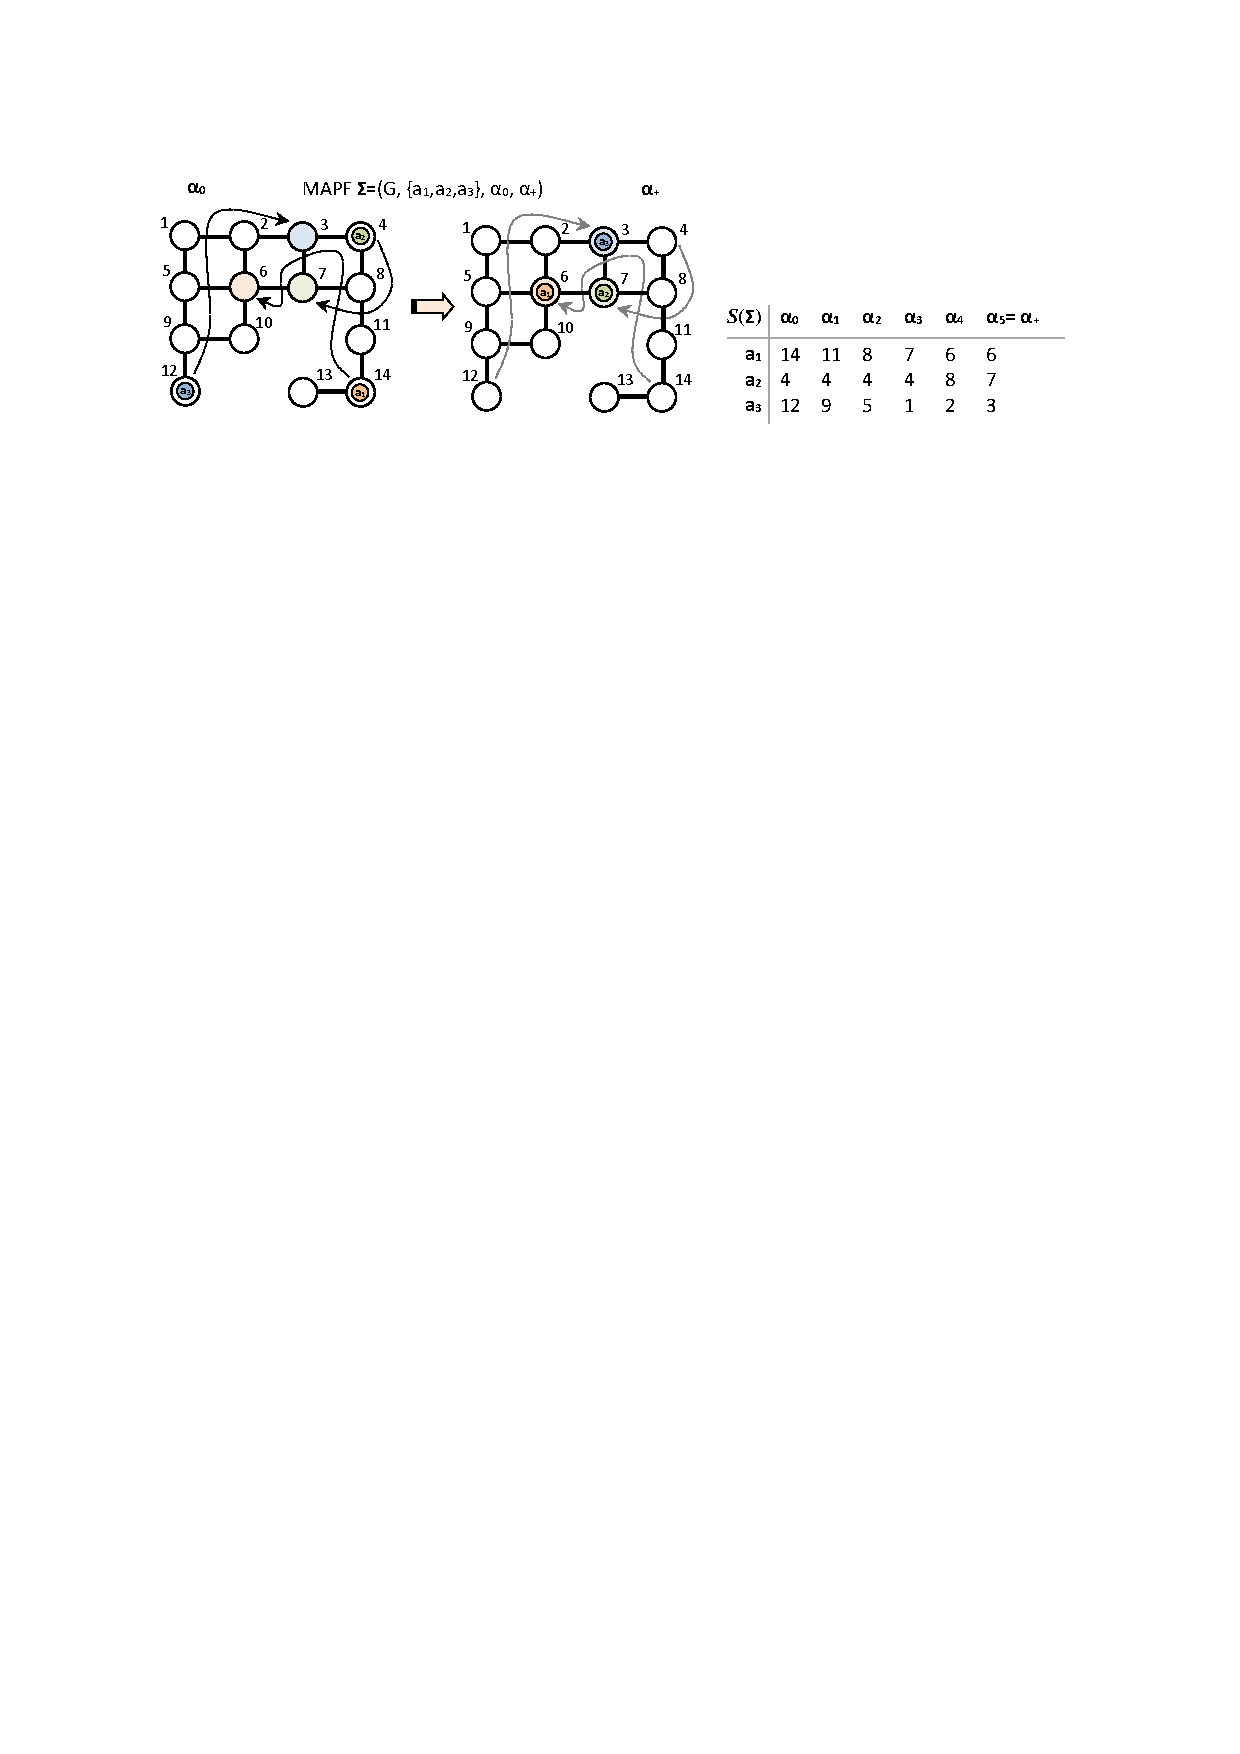
\includegraphics[trim={2.5cm 22.6cm 3cm 3.0cm},clip,width=1.0\textwidth]{fig_MAPF.pdf}
\caption{Example of MAPF problem instance for agents $a_1$, $a_2$, and $a_3$ over a
$4$-connected grid (left) and its solution (right).} \label{figure-MAPF}
\end{figure}

\noindent{\bf (1)  sum-of-costs} (denoted $\xi$) is the summation, over all
agents, of the number of time steps required to reach the goal
position~\cite{dresner2008aMultiagent,DBLP:conf/aaai/Standley10,DBLP:journals/ai/SharonSGF13,CBSJUR}.
Formally, $\xi = \sum_{i=1}^k{\xi(a_i)}$, where $\xi(a_i)$ is an
\textit{individual path cost} of agent $a_i$.
\vspace{0.25cm}


\noindent{\bf (2) makespan:} (denoted $\mu$) is the total time until the last
agent reaches its destination (i.e., the maximum of the individual
costs)~\cite{DBLP:conf/aaai/Surynek10,DBLP:conf/ictai/Surynek14,DBLP:conf/ijcai/Surynek15}.
\vspace{0.25cm}

It is important to note that in any solution $\mathcal{S}(\Sigma)$ it holds
that $\mu \leq \xi \leq {k\cdot\mu}$. Similarly it holds that the optimal \textit{makespan} is
smaller or equal to the optimal \textit{sum-of-costs} since otherwise the inequalities would be violated.

Intuitively, sum-of-costs can be regarded as the total energy consumption of all agents such that at each time step spent before reaching the goal the agent consumes one unit of energy. In this respect, it is not surprising that optimization of one of these two objectives goes against the other - total time can be saved at the cost of increased energy consumption and vice versa. An example of an MAPF instance where any makespan-optimal solution has sum-of-costs that is greater than the optimum and any sum-of-costs optimal solution has makespan that is greater than the optimal makespan is shown in Figure \ref{figure-MAKEvsCOST}.

\begin{figure}[t]
\centering
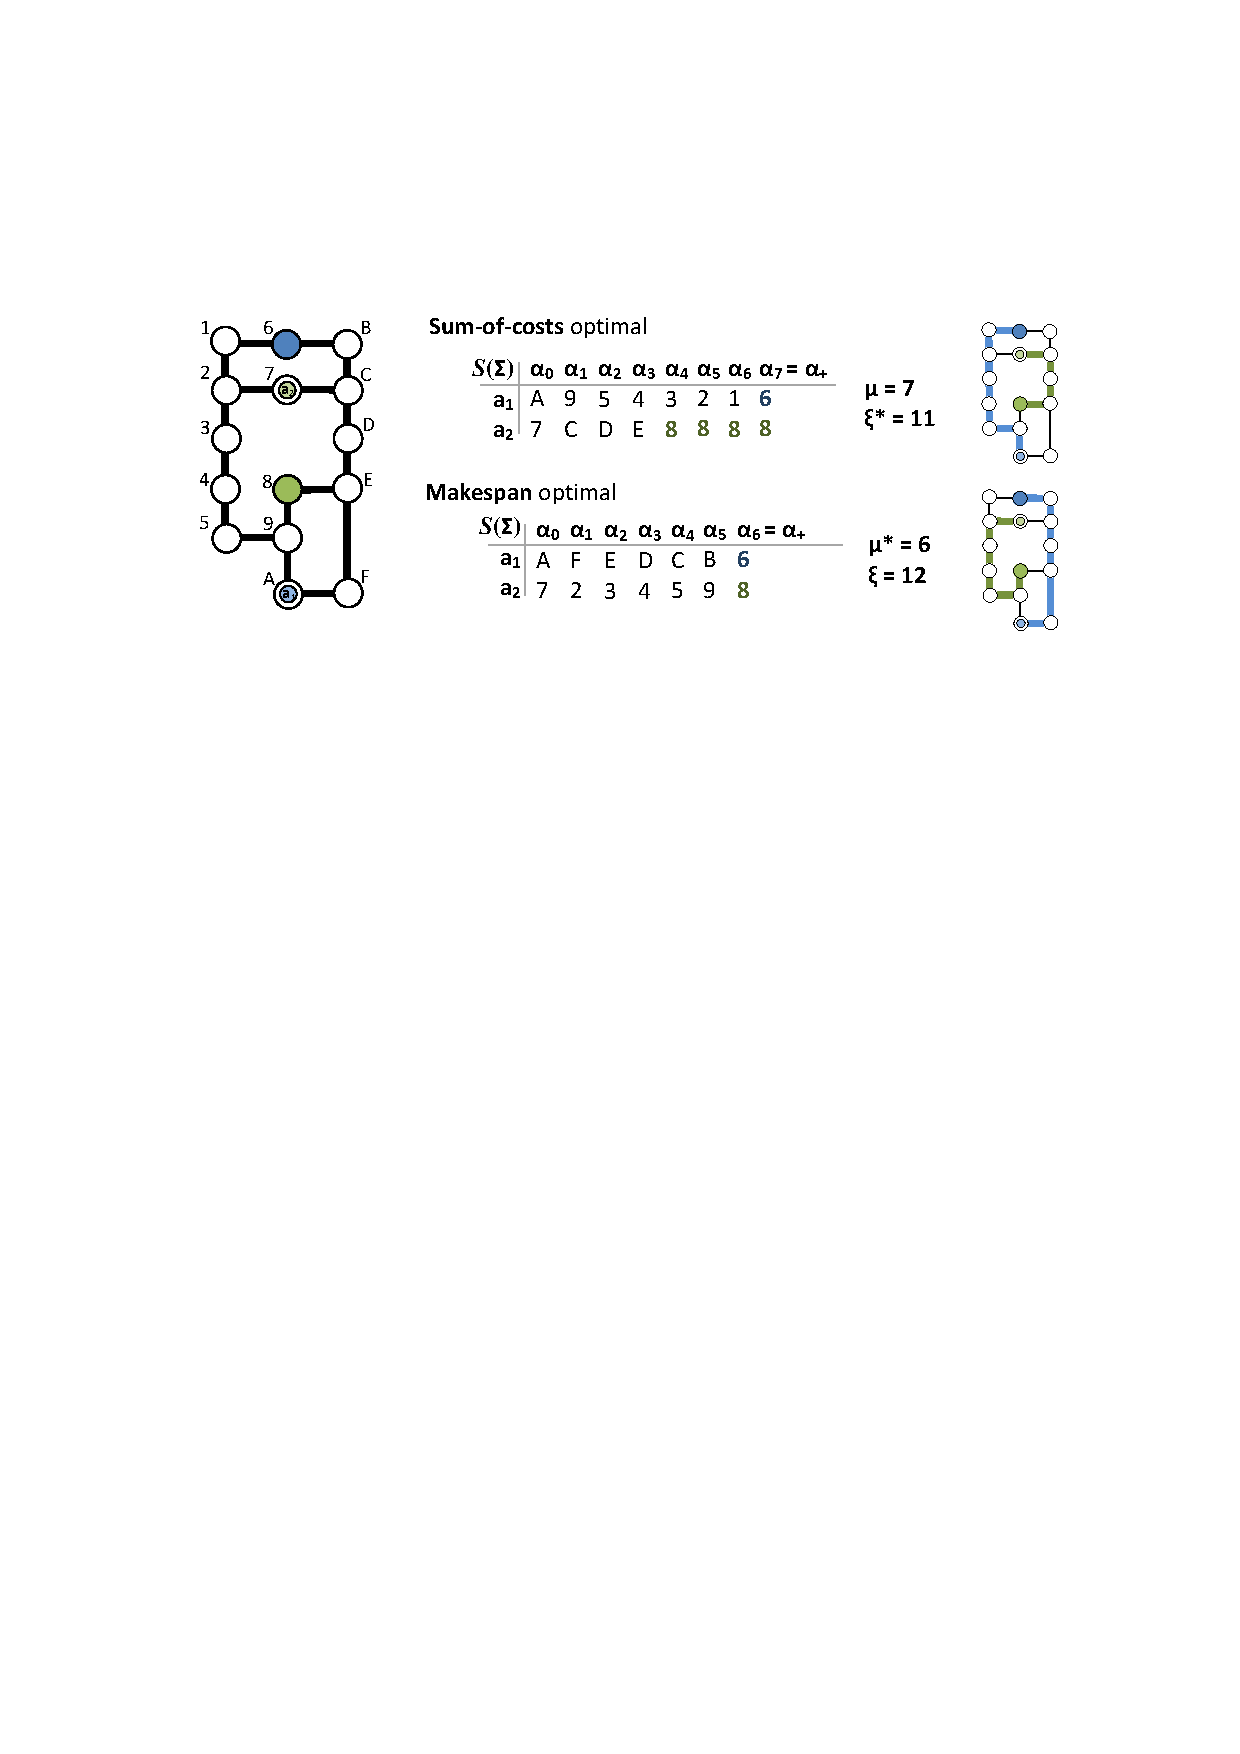
\includegraphics[trim={2.5cm 19.0cm 1.5cm 5.3cm},clip,width=1.0\textwidth]{fig_MAKEvsCOST.pdf}
\caption{An instance of MAPF where {\em makespan} and {\em
sum-of-costs} optimal solutions differ - that is, any makespan-optimal solution
is strictly sum-of-costs suboptimal and any sum-of-costs optimal solution is strictly makespan suboptimal.}
\label{figure-MAKEvsCOST}
\end{figure}

Finding optimal solutions for both variants with any standard style of agents' movement is
NP\nobreakdash-hard even on planar graphs~\cite{DBLP:conf/aaai/RatnerW86,DBLP:journals/jsc/RatnerW90,DBLP:conf/aaai/Surynek10,DBLP:journals/fuin/Surynek15,DBLP:conf/aaai/YuL13,DBLP:journals/ral/Yu16}. Therefore, many suboptimal solvers were developed, and are usually used, when the number of agents or the graph is very large~\cite{CohenUK15,KhorshidHS11,roger2012non,DBLP:conf/icra/Ryan10,DBLP:conf/aiide/Silver05,DBLP:journals/jair/WangB11}. In contrast to the difficulty of finding optimal solutions, finding any feasible solution or detecting unsolvability of a given instance can be done in polynomial time \cite{DBLP:journals/jair/WildeMW14,DBLP:conf/focs/KornhauserMS84,DBLP:conf/aaai/LunaB11,DBLP:conf/icra/Surynek09,DBLP:journals/ci/Surynek14}.


\subsection{Optimal MAPF Solvers}

Many optimal solvers were introduced in the past decade, most of which focus on
one of these cost functions:

\begin{itemize}

\item {\bf (1) Sum-of-costs.} Most optimal MAPF solvers that optimize this cost function are based on
search. Some of these search-based solvers are variants of the A* algorithm on
a global {\em search space} in which all different ways to place $k$ agents into $V$
vertices, one agent per vertex, are considered~\cite{DBLP:conf/aaai/Standley10,WagnerC15}.
Others employ novel search trees~\cite{DBLP:conf/ijcai/BoyarskiFSSTBS15,CBSJUR,DBLP:journals/ai/SharonSGF13}.
Search-based solvers feature various search-space pruning techniques like {\em independence detection} (ID) \cite{DBLP:conf/aaai/Standley10} or {\em multi-value decision diagrams} (MDDs) \cite{DBLP:journals/ai/SharonSGF13}.

\item {\bf (2) Makespan.} Many optimal solvers that optimize this cost function are {\em compilation-based solvers}, which means they solve MAPF by reducing it to known problems such as Constraint Satisfaction (CSP)~\cite{DBLP:conf/icra/Ryan10},
Boolean Satisfiability (SAT)~\cite{surynek2012towards}, Integer Linear
Programming (ILP) \cite{yu2013planning}, or Answer Set
Programming (ASP) \cite{erdem2013general}. These works mostly prove a
polynomial-time reduction from MAPF to these problems. 
Notably, these reductions are usually not directly applicable for the sum-of-costs variant. % This repeats the first statemetn 
%Existing reductions are usually designed for the {\em makespan} variant of MAPF; they are not directly applicable for the sum-of-costs variant. % This repeats the first statement, I re-phrased 

\end{itemize}

\subsection{Current Shortcomings and Contribution}

A major weakness across all these works is that each of these algorithms was
introduced and applied for one of these objective functions only. Furthermore,
the connection/comparison between different algorithms was usually done only
within a given class of algorithms but not across these two classes.
Finally, experiments were always performed on one objective-function
and very little is known on the performance and relevance of any given
algorithm (developed for one cost function) on the other objective function.

This paper aims to start to close the gap. First, we discuss how to migrate
algorithms across the different objective functions. Most of the search-based
algorithms developed for the sum-of-cost objective function can be modified to
the makespan variant with some technical adaptations such as modifying the cost
function and the way the state-space is represented. Some initial directions
are given by  Sharon et al. \citeyear{CBSJUR} and we give a complete picture here. 
By contrast, the compilation-based algorithms that were developed for the
makespan objective function are not trivially modified to the sum-of-costs
variant and sometimes a completely new encoding is needed.

A major algorithmic contribution of this paper is that we develop the first compilation-based solver
for the sum-of-costs variant to SAT. Our SAT-based solver is based on establishing relations between
the maximum makespan under the given sum-of-costs which enables to build SAT encodings that represent
all feasible solutions for the given sum-of-costs. Bounds on the sum-of-costs in the SAT encoding are established by
{\em cardinality constraints}~\cite{DBLP:conf/cp/BailleuxB03,DBLP:conf/cp/SilvaL07}. We show how to use known
lower bounds on the sum-of-costs to reduce the number of Boolean variables that encode these cardinality constraints so as to be practical for current SAT solvers.

We then present how to migrate various techniques used in search-based approaches to our new SAT-based solver.
First, we adapt ideas from the \textsc{Icts} algorithm~\cite{DBLP:journals/ai/SharonSGF13} that uses {\em multi-value decision diagrams} (MDDs)~\cite{DBLP:conf/iccad/SrinivasanKMB90} to further
reduce the size of SAT encodings. Next, we show how to integrate a modification of the {\em independence detection} technique \cite{DBLP:conf/aaai/Standley10} into the SAT-based solver. Finally, we demonstrate the flexibility of our SAT-based solver by modifying it into a bounded-suboptimal sum-of-costs solver - a modification applicable in search-based approaches to trade-off the quality of solutions for shorter runtime \cite{DBLP:conf/ecai/BarerSSF14}.

Successful migration of techniques demonstrates the potential of combining ideas from
both classes of approaches - search-based and compilation-based. Experimental results
show that our SAT solver with various enhancements outperforms the best existing search-based
solvers for the sum-of-costs variant on many scenarios.
Hence, as a result of our unification provided in the beginning of this paper,
we have a variety of algorithms which can be applied for both objective
functions. We conclude this paper by providing experimental results comparing
the hardness of solving MAPF with SAT-based and search-based solvers under the
makespan and the sum-of-costs objectives in a number of domains.


Results presented in this work partly appeared in several conference papers \cite{DBLP:conf/ecai/SurynekFSB16,DBLP:conf/socs/SurynekFSB16,DBLP:conf/socs/SurynekFSB17,DBLP:conf/icaart/SurynekSFB17a,DBLP:conf/icaart/SurynekSFB17}. 
Here we provide a significantly more comprehensive summarization and extension of these results. 
All SAT-based algorithms and encodings are described here in greater details, including detailed pseudo-codes. 
Detailed proofs of important properties such as completeness and time/space complexity are given. 
A broader context of how this work fits with existing works in classical planning, multi-agent planning, and planning using Markov Decision Processes is given. 
The experimental evaluation has been extended significantly, including experiments not reported in the conference papers that explore:
\begin{enumerate}[label=(\roman*)]
\item The impact of using a newer SAT solver on the ability of our algorithms to solve more MAPF problems;
\item The relation between the computed makespan and the number of time expansions needed to prove its optimality;
\item The distribution of runtime spent in each time expansion.
\end{enumerate}

% \roni{I editted the above, please see if you like this}
%and detailed proofs of properties of suggested concepts such as completeness, time/space complexity are given. Experimental evaluation is extended with benchmarks not reported in the conference papers. All algorithms are explained using detailed pseudo-codes. 




\subsubsection{Organization}

This paper is organized as follows. We first summarize related work on MAPF and introduce the context in which new methods are developed (section 2). Then a SAT-based solver for MAPF is introduced in several steps - starting with a basic solver (sections 3 and 4), which is further improved to obtain the final solver called MDD-SAT (section 5). A thorough experimental evaluation of MDD-SAT with respect to comparable search-based solvers is presented next (section 6). To further demonstrate the versatility of SAT-based approach, we show how to integrate independence detection into MDD-SAT (section 7) and how to build a bounded suboptimal solver using MDD-SAT (section 8) both with relevant experimental evaluation.

\section{Related Work}

We briefly summarize existing algorithmic approaches to MAPF in this section. We categorize algorithms into two streams according to the objective function they use. For optimization of {\em sum-of-costs} a great variety of algorithms has been proposed. On the other hand, previous {\em makespan}-optimal algorithms are limited to the compilation-based approach where the target formalism is represented by Boolean satisfiability. Many sum-of-costs optimal algorithms can be directly modified for the makespan variant. The opposite migration from the makespan-optimal case to the sum-of-costs optimality in compilation-based algorithms is however not straightforward. 

\subsection{Previous Sum-of-Costs Optimal Algorithms and Techniques}

{\bf A*-based Algorithms}. A* is a general-purpose algorithm that is well suited to solve MAPF. A common
straight-forward state-space where the states are the different ways to place $k$ agents into
$n=|V|$ vertices, one agent per vertex is used. In the {\em start} and {\em goal} states
agent $a_i$ is located at vertices $\alpha_0(a_i)$ and $\alpha_+(a_i)$, respectively. Operators
between states are all non-conflicting combinations of actions (including wait)
that can be taken by the agents.

The branching factor in A*-based algorithms is an important measure. Let $b(a_i)$ be the branching factor of single agent $a_i$. Then the {\em effective branching factor} for $k$ agents, denoted by $b$, is $b=\prod_{i=1}^k b(a_i)$. For example, in a 4-connected grid $b(a_i)=5$ for most of agents; an agent can either move in four cardinal directions or wait at its current position. Then $b$ is roughly ${5}^k$; though
usually a bit smaller because many possible combinations of moves result
in immediate conflicts, especially when the environment is dense with agents.

A simple admissible heuristic that is used within A* for MAPF is to sum
the individual heuristics of single agents such as the Manhattan distance for
4-connected grids or the Euclidean distance for Euclidean
graphs~\cite{ryan2008exploiting}. A more-informed heuristic is called the {\em
sum of individual costs} heuristic . For each agent $a_i$ we
calculate its optimal path cost from its current state to $\alpha_+(a_i)$ assuming
that other agents do not exist. Then, we sum these costs over all
agents. More-informed heuristics use forms of pattern-databases~\cite{DBLP:conf/socs/GoldenbergFSHS13,EPEJAIR}.

The most important drawback of A*-based algorithms is they need to tackle that the branching factor
$b$ of a given state may be exponential in $k$. We briefly summarize attempts to overcome the high branching factor.

{\bf Operator Decomposition (\textsc{Od}).} Instead of moving all the agents to their next positions
at once, agents advance to the next position one by one in a fixed order within the \textsc{Od} concept. The
original operator for obtaining the next state is thus decomposed into a sequence of operators for individual agents each of branching factor $b(a_i)$. \textsc{Od} together with a {\em reservation table} enabled computations of next states where agents do not collide with each other in \textsc{Ca*}, \textsc{Hca*}, and \textsc{Whca*} \cite{DBLP:conf/aiide/Silver05}.

Pruning of states by \textsc{Od} with respect to a given admissible heuristic was suggested by Standley \citeyear{DBLP:conf/aaai/Standley10}. Two conceptually different states are distinguished - {\em standard} and {\em intermediate}. The intermediate states correspond to the situation when not all the agents performed their move while the standard states correspond to states in the original representation with no \textsc{Od}.
The major strength of \textsc{Od} lies in the fact that the top-level A* algorithm does not need to distinguish
between standard and intermediate states. The next node for expansion is selected among both standard
and intermediate states while the cost function applies to both types of states. It may thus happen
that a certain intermediate state is not expanded towards a standard state because other states turned out
to be better according to the cost function. Such search space pruning cannot be done without
operator decomposition as there would be standard states only.

{\bf Independence Detection (\textsc{Id}).} Closely related to \textsc{Od} is the concept of {\em independence detection} \cite{DBLP:conf/aaai/Standley10}, which can be regarded as another branching factor reduction technique. The main idea behind this technique is that the difficulty of solving MAPF optimally grows exponentially with the number of agents. It would be ideal, if we could divide the problem into a series of smaller sub problems, solve them independently, and then combine them.
The simple approach, called simple independence detection (\textsc{Sid}), works as follows. First, it finds the shortest path for each agent to its goal, ignoring all other agents. 
Every pair of these single-agent paths is checked for conflicts (that is, when a collision between the agents will occur if they follow these paths concurrently). If a conflict is found, these agents are grouped together and a new optimal solution is found for the resulting group. This process continues, merging conflicting agents or groups of agents into larger groups until a set of solutions are found that do not conflict. This approach can be further improved by deliberately attempting to avoid the merging of groups.

{\bf More A*-based Algorithms.} Enhanced Partial Expansion (\textsc{Epea*}) \cite{EPEJAIR} avoids
the generation of surplus nodes by using {\em a priori} domain knowledge.
When expanding a node $N$ \textsc{Epea*} generates only the children $N_c$ with
$f(N_c)=f(N)$. The other children of $N$ (with $f(N_c) \neq f(N)$) are
discarded. This is done with the help of a domain-dependent {\em operator
selection function} (OSF)~\cite{EPEJAIR}.

M*~\cite{WagnerC15} and its enhanced recursive variant (\textsc{rM*}) are important
A*-based algorithms related to ID. M* dynamically changes the {\em
dimensionality} and branching factor based on conflicts. The dimensionality is
the number of agents that are not allowed to conflict. When a node is expanded,
M* initially generates only one child in which each agent takes (one of) its
individual optimal moves towards the goal (dimensionality 1). This continues
until a conflict occurs between $q \geq 2$ agents at node $N$. At this point,
the dimensionality of all the nodes on the branch leading from the root to $N$
is increased to $q$ and all these nodes are placed back in the OPEN list. When one of
these nodes is re-expanded, it generates $b^q$ children where the $q$
conflicting agents make all possible moves and the $k-q$ non-conflicting agents
make their individual optimal move.

An enhanced variant of M* called \textsc{ODrM*}~\cite{DBLP:conf/icra/FernerWC13} builds
\textsc{rM*} on top of Standley's \textsc{Od} rather than plain A*.

\textbf{Increasing Cost Tree Search.} The {\em increasing cost tree search} algorithm (\textsc{Icts})~\cite{DBLP:journals/ai/SharonSGF13} is a two-level MAPF solver that is conceptually different from A*. This algorithm is particularly important as its concepts will be be migrated into the SAT framework we are about to introduce. \textsc{Icts} works as follows.

At its {\em high level}, \textsc{Icts} searches the {\em increasing
cost tree} (\textsc{Ict)}. Every node in \textsc{Ict} consists of a $k$-ary vector $[C_1,
\ldots C_k]$, which ``represents {\em all} possible solutions in which the individual path cost of agent $a_i$ is exactly $C_i$''~\cite{DBLP:journals/ai/SharonSGF13}. The root of \textsc{Ict} is
$[opt_1,...,opt_k]$, where $opt_i$ is the optimal individual path cost for
agent $a_i$ ignoring other agents, i.e., it is the length of the shortest path
from $\alpha_0(a_i)$ to $\alpha_+(a_i)$ in $G$.

A child in \textsc{Ict} is generated by increasing the cost for one of the agents by 1. An \textsc{Ict} node $[C_1,..,C_k]$ is a {\em goal} if there is a complete non-conflicting solution such that the cost of the
individual path for any agent $a_i$ is exactly $C_i$. Figure~\ref{figure-ICT}
illustrates an \textsc{Ict} with 3 agents, all with optimal individual path costs of 10.
Dashed lines mark duplicate children which can be pruned. The total cost of a
node is $C_1+ \ldots +C_k$. For the root this is exactly $opt_1
+ opt_2 + \ldots opt_k$. Since all nodes at the same height have the same total cost, a breadth-first search of
the \textsc{Ict} will find the optimal solution.

\begin{wrapfigure}{r}{0.5\textwidth}
\begin{center}
\includegraphics*[height=2.4cm]{fig_ICT.pdf}
\end{center}
\vspace{-0.4cm}
\caption{Increasing cost tree (\textsc{Ict}) for three agents.} \label{figure-ICT}
\end{wrapfigure}

The \emph{low level} acts as a goal test for the \emph{high level}. For each
\textsc{Ict} node  $[C_1,..,C_k]$  visited by the \emph{high level}, the \emph{low level} is invoked.
Its task is to find a non-conflicting complete solution such that the cost of
the individual path of agent $a_i$ is exactly $C_i$. For each agent $a_i$, \textsc{Icts}
stores {\em all} single-agent paths of cost $C_i$ in a special compact
data-structure called a {\em multi-value decision diagram}
(MDD)~\cite{DBLP:conf/iccad/SrinivasanKMB90}.

The \emph{low level} searches the cross product of the MDDs in order to find a set of
$k$ non-conflicting paths for the different agents. If such a non-conflicting
set of paths exists, the \emph{low level} returns {\em True} and the search halts.
Otherwise, {\em False} is returned and the \emph{high level} continues to the next
high-level node (of a different cost combination).

\textsc{Icts} also implements various pruning rules to enhance the search. These pruning rules and their connection to CSP was also studied~\cite{DBLP:journals/ai/SharonSGF13}.

{\bf Conflict-based Search (\textsc{Cbs}).} Another optimal MAPF solver not based on A* is {\em conflict-based
search} (\textsc{Cbs})~\cite{CBSJUR}. In \textsc{Cbs}, agents are associated with constraints. A {\em constraint} for agent
$a_i$ is a tuple $\langle a_i,v,t \rangle$ where agent $a_i$ is prohibited from
occupying vertex $v$ at time step $t$. A {\em consistent path} for agent $a_i$ is a path that satisfies {\em all} of $a_i$'s constraints, and a {\em consistent solution} is a solution composed of only consistent paths. 

Once a consistent path has been found for each agent, these paths are {\em validated} with respect to the other agents by simulating the movement of the agents along their planned paths.

If all agents reach their goal without any conflict the solution is returned. If, however, while performing the
validation, a conflict is found for two (or more) agents, the validation halts and a conflict is resolved by adding constraints.
If a \emph{conflict}, $\langle a_i,a_j,v,t \rangle$ is encountered, that is agents $a_i$ and $a_j$ collide in vertex $v$ at time $t$, we know that in any valid solution at most one of the conflicting agents, $a_i$ or $a_j$, may occupy vertex $v$ at time $t$.
Therefore, at least one of the constraints, $\langle a_i,v,t \rangle$ or $\langle a_j,v,t \rangle$, must be satisfied. Consequently, \textsc{Cbs} {\em splits} the search into two branches where one of these constraints is imposed in each branch.

\subsection{Previous Makespan-Optimal Algorithms for MAPF}

A major development in makespan-optimal MAPF solving has been done under the Boolean satisfiability (SAT) \cite{Biere:2009:HSV:1550723} compilation paradigm. Early works that
compile MAPF to SAT focused on solution improvements in terms of shortening the makespan towards the optimum in an {\em anytime} manner \cite{DBLP:conf/pricai/Surynek12}. First, a makespan-suboptimal solution of the input MAPF is generated by a fast polynomial rule-based algorithm like \textsc{Bibox} \cite{DBLP:journals/ci/Surynek14} or \textsc{Push-and-Swap} \cite{DBLP:conf/aaai/LunaB11,DBLP:conf/atal/WildeMW13}. Then continuous sub-sequences of time steps in the current solution are replaced by makespan-optimal ones. The length of replaced sub-sequences is increased in each iteration of the algorithm until it eventually covers the entire makespan. This ensures that given enough time the algorithm returns a makespan-optimal solution. A suboptimal solution is available at any stage of the algorithm.

{\bf \textsc{Inverse} SAT encoding.} Historically the first encoding of MAPF to SAT \textsc{Inverse} relies on {\em log-space} encoded finite domain variables \cite{DBLP:books/sp/Petke15} that represent what agent is located at vertex $v$ at each time step $t$ - that is, the inverse $\alpha_t^{-1}:V \rightarrow A \cup \{\bot\}$ of $\alpha:A \rightarrow V$ (where assigning $\bot$ to a vertex means no agent is located at that vertex) is represented using log-space encoded bit-vectors $\mathcal{A}_t^{v} \in \{0,1,2,...,k\}$. MAPF movement rules and state transitions are encoded by a number of constraints over $\mathcal{A}_t^{v}$ \cite{DBLP:conf/pricai/Surynek12}. Altogether Boolean formula $\mathcal{F}_{\mu}$ is constructed on top $\mathcal{A}_t^{v}$ Boolean variables such that it is satisfiable if and only if a solution to the input MAPF of makespan $\mu$ exists. The advantage of this encoding is that the {\em frame problem} \cite{McCHay69} of propagation of agents' positions to the next time step can be easily done by enforcing equalities between $\mathcal{A}_t^{v}$ and $\mathcal{A}_{t+1}^{v}$ (bit-wise equality for all bits of a pair of log-space encoded variables).

Further works in SAT-based approach to MAPF \cite{DBLP:conf/iros/Surynek13,DBLP:conf/sara/Surynek13} omitted the phase in which suboptimal solution was improved and a makespan-optimal solution was generated directly instead. The process of finding a makespan-optimal solution follows the scheme described in Algorithm \ref{alg-MAPF-SAT-make}. Assuming a solvable MAPF instance, a makespan-optimal solution is obtained by answering satisfiability of $\mathcal{F}_{\mu_0},\mathcal{F}_{\mu_0+1}, ...$ until a satisfiable formula is found. The search starts with $\mu_0$, the lower bound on makespan obtained as the length of longest path over all shortest paths connecting starting position $\alpha_0(a_i)$ and goal $\alpha_+(a_i)$ of each agent $a_i$. The first satisfiable $\mathcal{F}_{\mu}$ represents the optimal makespan and an optimal solution can be extracted from its satisfying assignment.

\begin{algorithm}[t]
\begin{footnotesize}
\SetKwBlock{NRICL}{Solve-MAPF-SAT$_{MAKESPAN}$($G=(V,E),A,\alpha_0,\alpha_+)$}{end} \NRICL{
    $\pi \gets$ $\{$shortest path from $\alpha_0(a_i)$ to $\alpha_+(a_i)\;|\;i = 1,2,...,k\}$ \\
    $\mu \gets \max_{i=1}^k{(length(\pi(a_i)))}$ \\
    \While {$\mathit{TRUE}$}{
        $\mathcal{F}(\mu) \gets$ encode$(\mu,G,A,\alpha_0, \alpha_+)$\\
        $assignment \gets$ consult-SAT-Solver$(\mathcal{F}(\mu))$\\
        \If {$assignment \neq$ UNSAT}{
        	$\pi \gets$ extract-Solution$(assignment)$\\
        	\Return $\pi$\\
        }
        $\mu \gets \mu + 1$\\
    }
} \caption{Framework of makespan-optimal SAT-based MAPF solving}
\label{alg-MAPF-SAT-make}
\end{footnotesize}
\end{algorithm}

\begin{wrapfigure}{l}{0.54\textwidth}
%\begin{figure}
\begin{center}
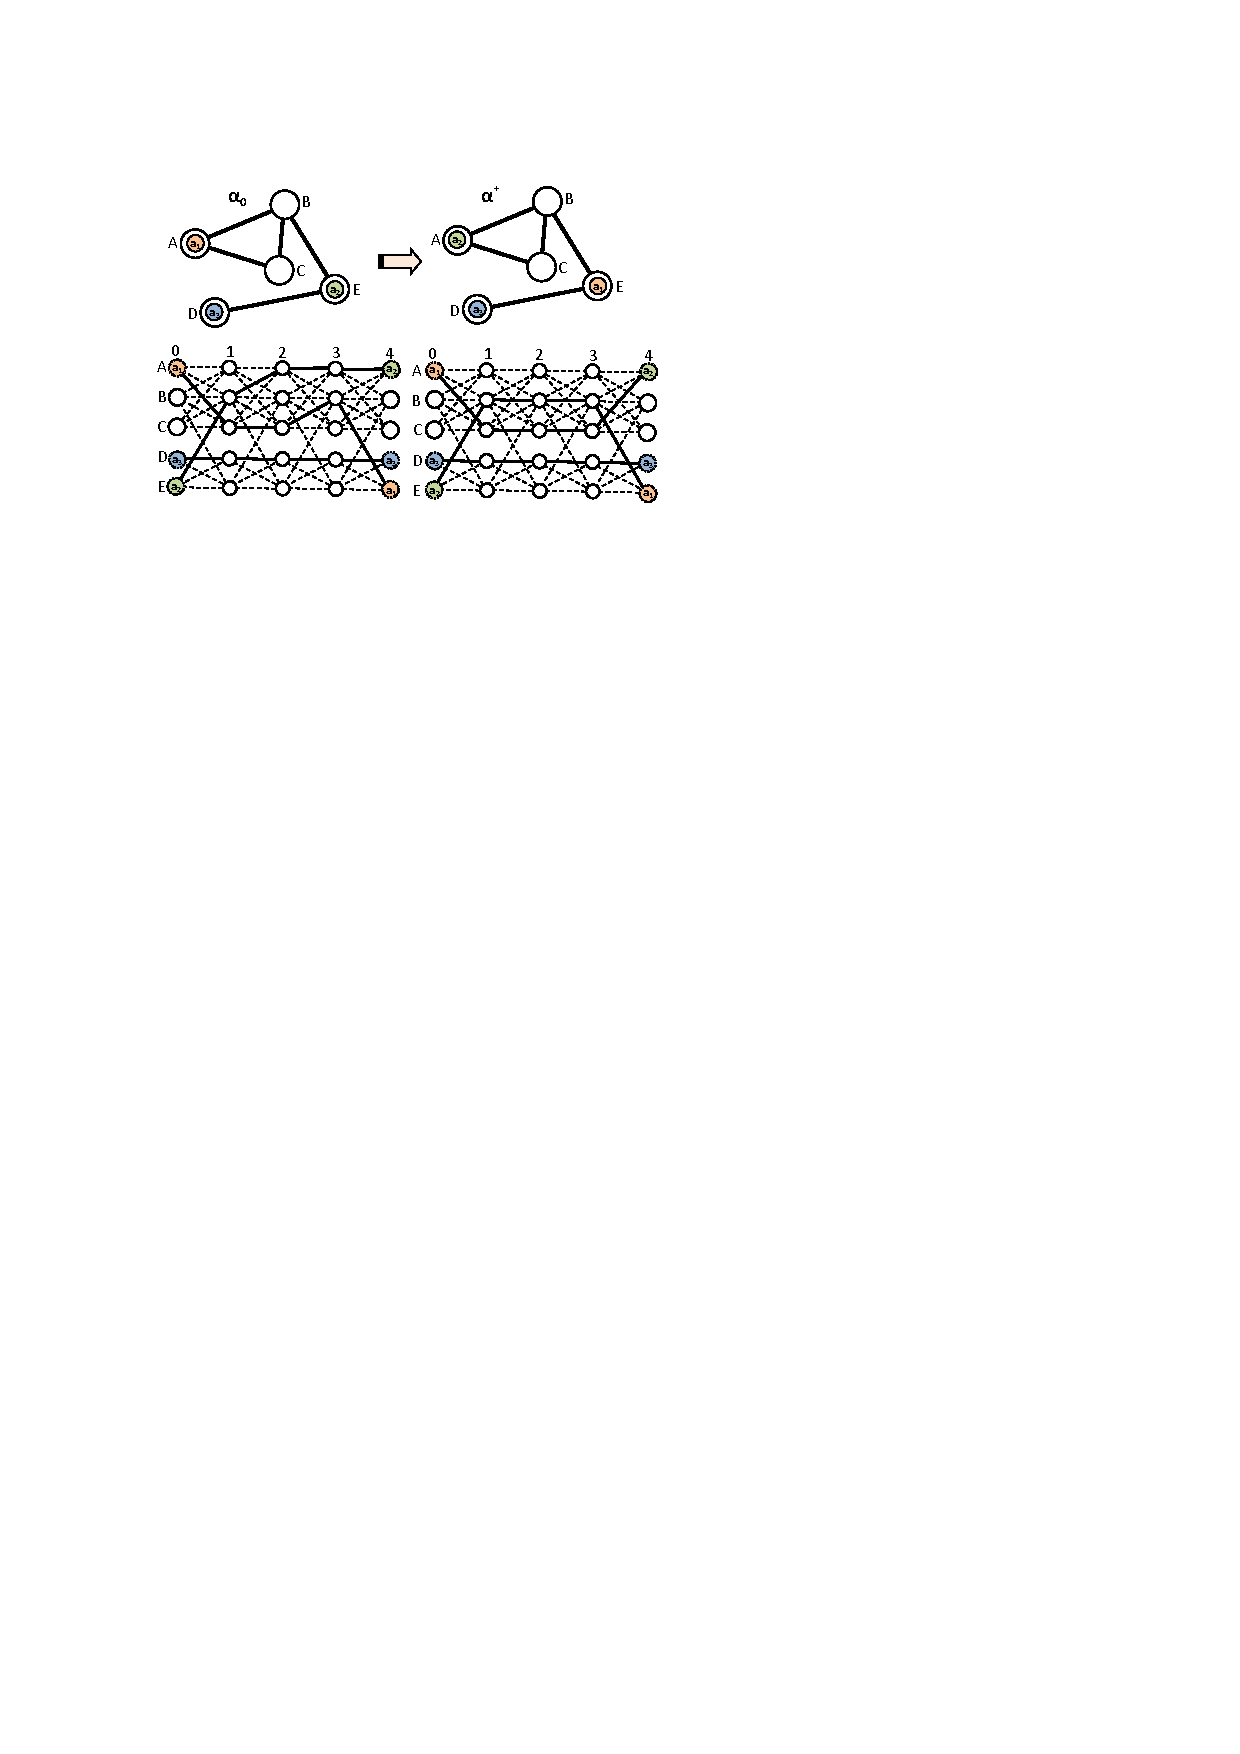
\includegraphics[trim={2.5cm 21cm 5.5cm 3cm},clip,width=0.8\textwidth]{fig_matching.pdf}
\end{center}
%\vspace{0.2cm}
\caption{Searching of non-conflicting paths over anonymized agents - conflicts are reflected but an agent may end up in the wrong goal (lower right part).} \label{figure-matching}
%\end{figure}
\end{wrapfigure}

\textbf{\textsc{All-Different} SAT encoding.} The \textsc{All-Different} encoding again employs the log-space representation of finite domain variables \cite{DBLP:conf/ictai/Surynek12}. The position of agent $a_i$ at time step $t$, that is, $\alpha_t$ is represented instead of representing vertex occupancy - that is, finite domain variables $\mathcal{D}_t^{a_i} \in V$ are represented using log-space encoding. To ensure that conflicts among agents at vertices do not occur, the \textsc{All-Different} constraint \cite{DBLP:conf/aaai/Regin94} is introduced for $\mathcal{D}_t^{a_i}$ variables over all agents for each time step $t$. The advantage of the \textsc{All-Different} encoding is that various efficient encodings of the \textsc{All-Different} \cite{DBLP:conf/fmcad/BiereB08,DBLP:conf/ecai/Surynek12} constraint over bit vectors can be integrated.

\textbf{\textsc{Matching} SAT encoding.} The next development has been done in SAT encoding called \textsc{Matching} that separates conflict rules in MAPF and agents transitions between time steps \cite{DBLP:conf/ictai/Surynek14}. Conflict rules are expressed over anonymized agents that are encoded by {\em direct} variables $\mathcal{M}_t^v \in \{\mathit{TRUE}, \mathit{FALSE}\}$ \cite{DBLP:journals/constraints/TamuraTKB09}.

The presence of some agent in vertex $v$ at time step $t$ is indicated by a single propositional variable ($\mathcal{M}_t^v = \mathit{TRUE}$ if and only if $\exists a_i \in A$ such that $\alpha_t(a_i)=v$). Using anonymized agents is however not enough as agents may end up in other agent's goal - see Figure \ref{figure-matching}. For transitions where individual agents need to be distinguished, log-space encoded variables $\mathcal{A}_t^v \in \{0,1,2,...,k\}$ represent what agent occupies a given vertex ($\mathcal{A}_t^v$ if and only if $\alpha_t(a_i)=v$) \cite{DBLP:conf/ictai/Surynek14}. The advantage of \textsc{Matching} over previous encodings \textsc{Inverse} and \textsc{All-Different} is that movement conflict rules can be expressed in a simpler way over direct variables $\mathcal{M}_t^v$ for anonymized agents. Compared to doing so over log-space encoded variables $\mathcal{A}_t^{v}$ or $\mathcal{D}_t^{a_i}$ that distinguish individual agents, smaller formula can be obtained with conflict reasoning over $\mathcal{M}_t^v$.

{\bf \textsc{Direct} SAT encoding.} Lessons taken from the previous development was that introduction of directly encoded variables leads to significant performance improvements although encoding set of states by direct variable is not as space efficient as the in the log-space encoding case. The next encoding purely based on direct variables - called \textsc{Direct} MAPF encoding \cite{DBLP:conf/micai/Surynek14} - introduces a single Boolean variable for every triple of agent, vertex, and time step; formally there is a Boolean variable $\mathcal{X}(a_i)_t^v$ such that it is $\mathit{TRUE}$ if and only if agent $a_i$ occupies $v$ at time step $t$  (some triples may be forbidden as unreachable). In this work we are partly inspired by the \textsc{Direct} encoding as for the idea of directly encoded variables. 

{\bf ASP, CSP, and ILP approach.} Although much work in makespan-optimal solving has been done for SAT, other compilation-based approaches to MAPF like ASP-based \cite{erdem2013general} and CSP-based \cite{DBLP:conf/icra/Ryan10} exist. Both ASP and CSP offer rich formalism to express various objective functions in MAPF. The ASP-based approach adopts a more specific definition of MAPF where bounds on lengths of paths for individual agents are specified as a part of the input. Except the bound on sum-of-costs the ASP formulation works with other constraints such as {\em no-cycle} (the agent shall not visit the same part of the environment multiple times), {\em no-intersection} (only one agent visits each part of the environment), or {\em no-waiting} (when minimization of idle time is desirable). The ASP program for a given variant of MAPF consisting of a combination of various constraints is solved by the \textsc{Clasp} SAT solver \cite{DBLP:conf/lpnmr/GebserKNS07a}.

Ryan~\citeyear{DBLP:conf/icra/Ryan10} proposed a CSP-based approach that focuses on the structure of the underlying graph $G$. The graph is partitioned into {\em halls} (singly-linked chain of vertices with any number of entrances and exits) and {\em cliques} (represents large open spaces with many entrances and exists) commonly referred to as sub-graphs. The plan is searched using CSP techniques over an abstract graph whose nodes are represented by the sub-graphs. Specific properties of different sub-graphs are reflected in the constraints - for example, agents in a clique sub-graph usually cannot exceed the capacity of the clique while in a hall sub-graph the agents must preserve their ordering. The resulting CSP is eventually solved using the \textsc{Gecode} solver \cite{Tack:PhD:2009}.

The similarity of MAPF and multi-commodity flows has also been studied~\cite{DBLP:conf/aaai/YuL13}, where each agent is regarded as a different commodity of a multi-commodity flow. The individual depths of the multi-commodity flow are associated with individual time steps of MAPF solution. Finding optimal solutions of MAPF with respect to various objective functions can be then modeled as finding an optimal solution to a Integer Linear Programming (ILP) problem \cite{DBLP:conf/icra/YuL13}.


\subsection{Multi-agent Planning and Multi-robot Planning}

Multi-agent path finding can be understood as a specific problem in the wider paradigm of multi-agent planning (MAP) \cite{DBLP:journals/mags/WeerdtC09,DBLP:journals/csur/TorrenoOKS17}. Agents in MAP operate in a shared environment and fulfil a given common goal. To achieve the common goal the agents need to be assigned their individual goals. The planning phase in MAP needs to coordinate actions of individual agents so that they benefit from positive interactions and avoid harmful interactions \cite{DBLP:conf/iat/DimopoulosM06}.

There exist many diverse techniques for MAP including heuristic search-based techniques with various improvements like divide-and-conquer \cite{DBLP:conf/aaai/EphratiR94} as well as compilation-based techniques using SAT \cite{DBLP:journals/kbs/DimopoulosHM12} or classical planning \cite{DBLP:conf/iat/DimopoulosM06} as a target formalism.

An important issue in MAP is also the negotiation phase in which agents decompose the common goal and assign individual tasks. Popular source methods for negotiation in MAP are game theoretical methods such as combinatorial auctions \cite{DBLP:journals/eswa/RobuNPS11}, voting \cite{DBLP:conf/icmas/Rosenschein95}, and argumentation \cite{DBLP:conf/ecai/SapenaOT10}. Another important issue in MAP is that agents deliberately do not share their knowledge completely with other agents, referred to as privacy-preserving MAP \cite{DBLP:journals/kais/TozickaJKP16}.

MAPF as a special MAP task is greatly simplified as individual agents' goals are assigned as part of the input so the negotiation phase is missing in MAPF. On the other hand, there is a strong emphasis on avoiding the negative interactions during the planning phase in MAPF.

Natural motivation for multi-agent path finding on graphs rests in {\em multi-robot planning} and coordination \cite{CHAI2013129,DBLP:journals/arobots/JonesDS11} (MRPC). The MRPC task consists in determining actions for a team of robots so that the team can fulfill a given task by executing the actions by individual robots. It is important that robots in the team collaborate with each other to fulfill the task, for example certain actions may require multiple robots to be executed.

One stream of research in MRPC focuses on heterogeneous teams of mobile robots \cite{Parker94}, the team usually consists of a small number of robots. Typical applications are search and rescue operations \cite{soton411031} with multiple robots each with different abilities to perform relatively complex actions \cite{DBLP:journals/arobots/JorgensenCMP18}. The other stream of works focuses on homogeneous teams of mobile robots \cite{DBLP:journals/automatica/OhPA15}. The homogeneous teams typically consist of larger number of robots but individual robots can perform only simpler actions such as motion and actions like loading and unloading.

MAPF appears in MRPC as a sub-problem when robots need to plan their paths to reach destinations where actions are performed. Physical occupation of space by robots in MRPC can be modeled by MAPF rules so collision free planning can be carried out via MAPF. In the case of homogeneous teams, the MAPF problem can represent even the whole phases of the MRPC such as in the case of motion planning for swarms of UAVs \cite{DBLP:journals/ijrr/KumarM12,DBLP:conf/swarm/SorliGB17}.

% Refer some related works from multi-agent planning and multi-robot planning related to MAPF. DONE

\section{SAT-Based Solvers for Makespan-Optimal MAPF}

\noindent SAT-based MAPF solvers reduce the question of existence of a solution to given MAPF instance to the Boolean satisfiability problem (SAT) \cite{Biere:2009:HSV:1550723}. The reduction encompasses Boolean variables to model the MAPF problem. As Boolean satisfiability answers binary questions the challenge is to apply SAT for MAPF where there is a cumulative cost function. A general scheme for using SAT solvers to solve an optimization problem is to reduce the optimization problem into a sequence of decision problems. The questions are {\em which decision problem to encode}, {\em how to encode it},  and {\em how to devise an appropriate sequence of these decision problems} that will guarantee a solution to the optimization problem at hand.


This challenge is stronger for the sum-of-costs variant where each agent has its own cost. We first recall concepts from SAT encodings for the makespan objective. Then, we present our SAT encoding for sum-of-costs.

% \subsection{SAT Encoding for Optimal Makespan}


A {\em time expansion graph} (denoted TEG) is a basic concept used by SAT-based MAPF solvers \cite{DBLP:conf/ictai/Surynek14,DBLP:conf/ecai/SurynekFSB16}. We use it too in the sum-of-costs variant below. A TEG is a directed acyclic graph (DAG). First, the set of vertices of the underlying graph $G$ are duplicated for all time-steps from 0 up to the given makespan bound $\mu$. Then, possible actions (move along edges or wait) are represented as directed edges between successive time steps. Figure~\ref{figure-TEG} shows graph $G=(V,E)$ and its TEG of depth 2 for time steps 0, 1 and 2 (vertical layouts) denoted $TEG(2)$. Copies of the underlying graph $G$ within TEG will be called {\em layers}.

It is important to note that in this example (1) horizontal edges in TEG correspond to {\em wait} actions. (2) diagonal moves in TEG correspond to real moves. Formally a TEG is defined as follows:

\begin{wrapfigure}{r}{0.5\textwidth}
\begin{center}
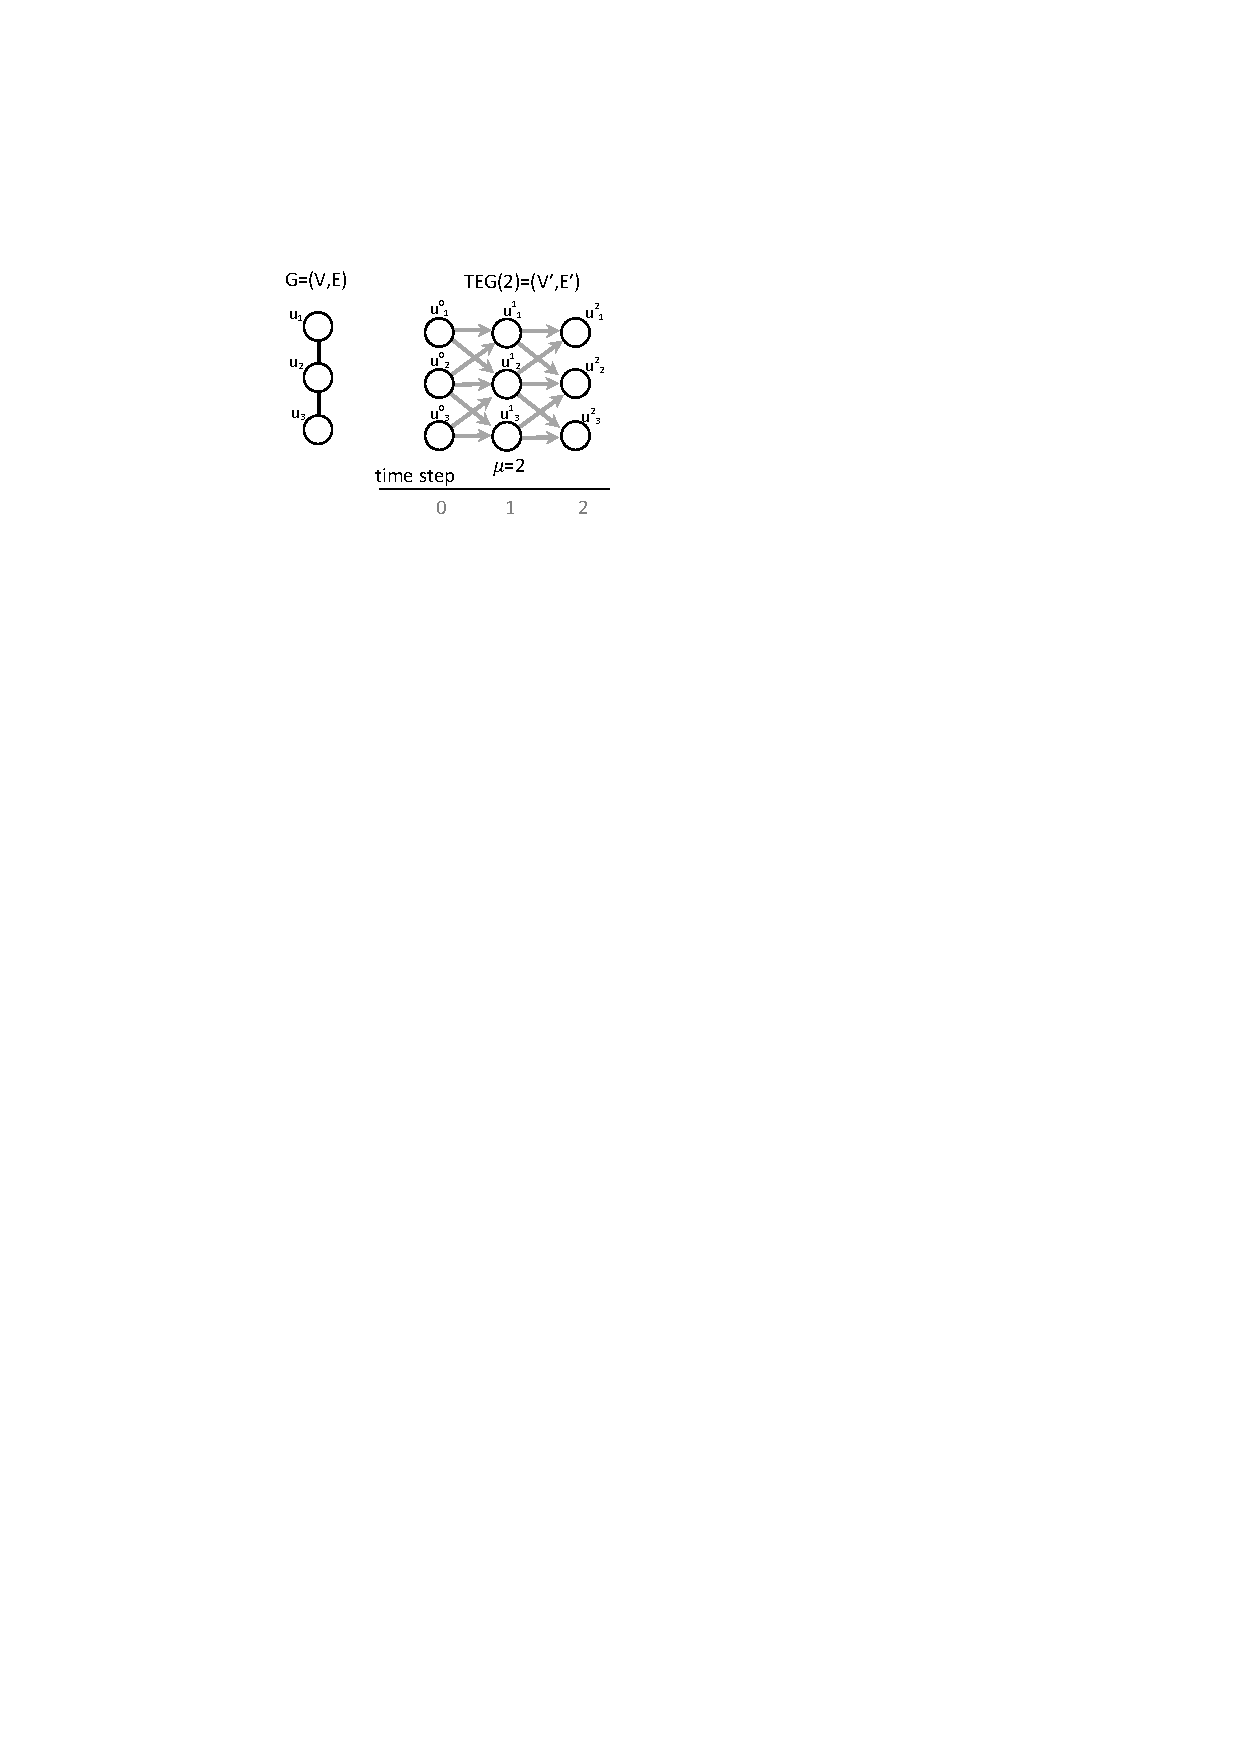
\includegraphics[trim={4.5cm 21.0cm 10.5cm 4.5cm},clip,width=0.4\textwidth]{fig_TEG.pdf}
\end{center}
\caption{An example of time expansion graph: input graph (left) and its expansion for 3 steps (depth 2). For each vertex $u_j \in V$ its copy $u_j^t$ indexed by time step $t$ is introduced and corresponding directed edges are added between successive time steps to represent actions including wait actions. } \label{figure-TEG}
\end{wrapfigure}

\begin{definition}
{\bf Time expansion graph} of depth $\mu$ corresponding to undirected graph $G=(V,E)$ is a digraph $\mathit{TEG}(\mu)=(V',E')$ where
$V'=\{u^t_j \;|\; t=0,1,...,\mu \wedge u_j \in V\}$ and $E'=\{{(u_j^t,u_l^{t+1})}\;|\; t=0,1,...,\mu-1\ \wedge (\{u_j,u_l\} \in E
\vee j=l) \}$. \label{def:TEG}
\end{definition}

The encoding for MAPF introduces TEGs for individual agents. That is, we have $TEG_i(\mu)=(V_i,E_i)$ for each agent $a_i \in \{1,2,...,k\}$. Directed non-conflicting paths in TEGs correspond to valid non-conflicting movements of agents in the underlying graph $G$. The existence of non-conflicting paths in TEGs is encoded as satisfiability of a Boolean formula. Next, we describe in more details the encoding style used in the \textsc{Direct} encoding.

Boolean variables and constraints (clauses) for a single time step $t \in \{0,1,...,\mu\}$ in $TEG_i(\mu)$ represent any possible position of agent $a_i$ at time step $t$; that is, we have $\mathcal{X}(a_i)_v^t$ from the \textsc{Direct} encoding. Boolean variables for all TEGs together represent all possible configurations of agents from time step $0$ up to time step $\mu$. It is ensured by constraints that configurations of agents in consecutive time steps of TEGs correspond to valid actions: agent $a_i$ can appear in vertex $u_j^t$ if it can move there from the previous time step in $TEG_i$ along a directed edge, that is, if $a_i$ is in some $u_l^{t-1}$ such that $(u_l^{t-1},u_j^t) \in E_i$. We also have inter-TEG constrains ensuring that agents do not collide with each other (detailed list of constraints will be introduced lter for the sum-of-costs variant).

Given a desired makespan $\mu$, formula $\mathcal{F}_{\mu}$ represents the question of whether there is a collection of non-conflicting directed paths in $TEG_1$,...,$TEG_k$ of depth $\mu$ such that the first configuration equals to $\alpha_0$ and the last one equals to $\alpha_+$. The search for optimal makespan is done by iteratively incrementing $\mu=0,1,2...$ until a satisfiable formula $\mathcal{F}_{\mu}$ is obtained as shown in Algorithm \ref{alg-MAPF-SAT-make}.

This process ensures finding a makespan-optimal solution in case of a solvable input MAPF instance, since the satisfiability of $\mathcal{F}_{\mu}$ is a non-decreasing function of $\mu$. It is important to note that solvability of a given MAPF can be checked in advance by a fast polynomial algorithm like \textsc{Push-and-Rotate} \cite{DBLP:conf/atal/WildeMW13}. More information on SAT encoding for the makespan-optimal variant can be found in various studies \cite{DBLP:conf/ictai/Surynek14,DBLP:conf/pricai/Surynek14,DBLP:conf/micai/Surynek14}. The detailed transformation of a question of whether there are non-conflicting paths in TEGs will be shown in the following sections.

% \section{Basic-SAT for Optimal Sum-of-costs}
\section{SAT-Based Solvers for Sum-of-costs Optimal MAPF}
\noindent The general scheme described above for finding the optimal makespan is to convert the optimization problem (finding the minimal makespan) to a sequence of decision problems. The decision problem was: is there a solution of makespan $\mu$, and the sequence of decision problems was to increment $\mu$ until the minimal makespan is found. The {\em numeric objective function} to minimize, i.e., the makespan $\mu$ corresponds directly to the number of time expansions of the underlying graph $G$ in TEG. Thus, the decision problem corresponded to the existence of directed paths in TEGs satisfying additional constraints encoding the MAPF rules.

We apply an analogous scheme for finding the optimal sum-of-costs, converting it to a sequence of decision problems -- is there a solution of a given sum-of-costs $\xi$, and the sequence of decision problems is to increment $\xi$ until finding the minimal sum-of-costs.

It is important to note that an incremental strategy to obtain the optimal value of the objective function is suitable only when the cost of a query is exponential in $\mu$ or $\xi$. In the case of uniform query costs different strategies, like binary search, would be more suitable. This roughly holds in MAPF, as increasing $\mu$ corresponds to adding a fresh time step in the TEGs, which is reflected in the encoded Boolean formula by adding a number of variables and constraints proportional to the size of $G$.

Since the runtime of a SAT solver is exponential in the size of the input formula in the worst case we have that the runtime for answering $\mathcal{F}_{\mu}$ is exponential in $\mu$ in the worst case. In such a setup with incremental strategy, the cost/runtime of the last query is roughly the same as the total cost/runtime of previous queries in the worst case.  As we will see later, the same applies also for the sum-of-costs $\xi$.

However, encoding the decision problem for the sum-of-costs is more challenging than the makespan case, because one needs to both bound the sum-of-costs, but also to predict how many time expansions are needed. We address this challenge by using two key techniques described next: {\bf (1)} Cardinality constraint for bounding $\xi$ and {\bf (2)} Bounding the makespan.


\begin{itemize}
\item{
\noindent {\bf Cardinality constraints.} This is a technique from the SAT literature that enables counting and bounding a numeric cost in a Boolean formula \cite{DBLP:conf/cp/BailleuxB03,DBLP:conf/cp/SilvaL07,DBLP:conf/cp/Sinz05}. Technically this is done by counting and bounding the number of Boolean variables from a given set that are assigned $\mathit{TRUE}$. This consequently enables encoding in a Boolean formulate a constraint that bounds the sum-of-costs (details in Section~\ref{sec:detailedDescription}).
}

\item{
\noindent  {\bf Upper bound on the required time expansions.}  We show below how to compute for a given sum of cost value $\xi$ a value $\mu$ such that all possible solutions with sum-of-costs $\xi$ must be possible for a makespan of at most $\mu$ (details in Section~\ref{sec:boundingTheMakespan}). This enables encoding the decision problem of whether there is a solution of sum-of-costs $\xi$ by using a SAT encoding similar to the makespan encoding with $\mu$ time expansions. In other words, it will be sufficient to use TEGs of depth $\mu$ in order to represent all solutions that fits under the given sum-of-costs $\xi$.
}
\end{itemize}

In the following sections, we explain each of this techniques in detail, along with additional implementation details.

\subsection{Bounding $\xi$ via Cardinality Constraint}

% \subsection{The Relation Between Time Expansions and Sum-of-costs Bounds}
% \subsection{Sum-of-costs Bounds and Required Time Expansions}

% SAT can bound numbers
\noindent The SAT literature offers a technique for encoding a \textit{cardinality constraint} \cite{DBLP:conf/cp/SilvaL07,DBLP:conf/cp/Sinz05}, which allows calculating and bounding a numeric cost within the Boolean formula. Formally, for a bound $\lambda \in \mathbb{N}$ and a set of Boolean variables $X=\{x_1,x_2,...,x_m\}$ the \textit{cardinality constraint} $\leq_{\lambda}{\{x_1,x_2,...,x_m\}}$ is satisfied if and only if the number of variables from the set $X$ that are set to $\mathit{TRUE}$ is $ \leq \lambda$. There are various ways how to encode cardinality constraints in Boolean formulae. The standard approach is to simulate arithmetic circuits \cite{DBLP:conf/cp/BailleuxB03} within the formula (either using binary or unary representation of numbers encoded by vectors of Boolean variables).

% How to map agent actions to cardinality constraints
In our SAT encoding, we use such cardinality constraints to encode a constraint that upper bounds the sum-of-costs. Specifically, we map every agent's action to a Boolean variable, which is $\mathit{TRUE}$ if that action is performed in the plan. Then, we add cardinality constraint over these variables, thereby encoding a bound on the sum-of-cost of the plan. To find a plan with an optimal sum-of-cost, we use the general structure of the makespan SAT encoding, increasing this sum-of-cost bound by one in every iteration, until a solution is found. 

A challenge with such a SAT encoding is that we must set both the number of time expansions as well as the sum of cost bound in every iteration. We address below the challenge of how to connect these two factors -- the number of time expansions and the sum of cost bound. The explicit form of the cardinality constraint will be expressed later after we will define the Boolean variables that the cardinality constraint will bound.

% Thus, one can use the general structure of the makespan SAT encoding (which iterates over possible makespans), and add such a cardinality constraint on top. We address the challenge of how to connect these two factors together.

\subsection{Bounding the Makespan for the Sum of Costs}
\label{sec:boundingTheMakespan}

We compute how many time expansions $\mu$ are needed to guarantee that if a solution with sum-of-costs $\xi$ exists then it will be found within at most $\mu$ time expansions. In other words, in our encoding, the values we give to $\xi$ and $\mu$ must fulfill the following requirement:

\vspace{0.25cm}
\noindent{\em {\bf Requirement (R1):} All possible solutions with sum-of-costs $\xi$ must be
possible for a makespan of at most $\mu$.}
\vspace{0.25cm}

To find a $\mu$ value that meets (R1) for given $\xi$, we require the following definitions. Let $\xi_0(a_i)$ be the cost of the shortest individual path for agent $a_i$, and let
$\xi_0=\sum_{a_i\in A} \xi_0(a_i)$. $\xi_0$ is called the {\em sum of individual costs} (SIC) \cite{DBLP:journals/ai/SharonSGF13}. $\xi_0$ is an admissible heuristic for optimal sum-of-costs search algorithms, since $\xi_0$ is a lower bound on the minimal sum-of-costs. $\xi_0$ is calculated by relaxing the problem by omitting the other agents.

Similarly, we define $\mu_0=\max_{a_i\in A} \xi_0(a_i)$.  $\mu_0$ is length of the {\em longest} of the shortest individual paths and is thus a lower bound on the minimal makespan. Finally, let $\Delta$ be the extra cost over SIC. That is, let $\Delta =  \xi - \xi_0$.

\newtheorem{proposition}{Proposition}
\begin{proposition}
For makespan $\mu$ of any solution with sum-of-costs $\xi$, where $\xi = \xi_0 + \Delta$, it holds that $\mu \leq \mu_0 + \Delta$. Hence (R1) is satisfied for setting $\mu = \mu_0 + \Delta$. \label{prop:upperbound}
\end{proposition}

\noindent {\bf Proof:} The worst-case scenario, in terms of makespan, is that all the $\Delta$ extra moves belong to a single agent. Given this scenario, in the worst case, $\Delta$ is assigned to the agent with the largest shortest-path. Thus, the resulting path of that agent would be $\mu_0+\Delta$, as required. $\Box$
% Make this more rigorous: "the worst case, in terms of makespan, happens when all the ? extra moves are assigned to the agent with the largest shortest-path"

\vspace{0.25cm}

% [[Original version]]
Using Proposition~\ref{prop:upperbound}, we can safely encode the decision problem of whether there is a solution with sum-of-costs $\xi$, knowing that if a solution of cost $\xi$ exists then it will be found within $\mu=\mu_0+\Delta$ time expansions. In other words, Proposition~\ref{prop:upperbound} shows the relation between the parameters $\mu$ and $\xi$, which will both be changed by changing $\Delta$.

% [[New version]]
% Using Proposition~\ref{prop:upperbound}, we can safely encode the decision problem of whether there is a solution with sum-of-costs $\xi$, knowing that if a solution of cost $\xi$ exists then it will be found within $\mu=\mu_0+\Delta$ time expansions. In other words, Proposition~\ref{prop:upperbound} shows relation of both parameters $\mu$ and $\xi$ which will be both changed by changing $\Delta$.

Algorithm~\ref{alg-MAPF-SAT-soc} summarizes our optimal sum-of-costs algorithm. In every iteration, $\mu$ is set to $\mu_0+\Delta$ (line 7) and the relevant TEGs of depth $\mu$ for various agents are built (these TEGs also take into account the minimum individual cost $\xi^i_0 = \xi_0(a_i)$ of individual agents $a_i$, described below). Using TEGs of individual agents a formula  $\mathcal{F}(\mu_0, \xi_0, \Delta)$ is constructed that encodes a decision problem whether there is a solution with sum-of-costs $\xi=\xi_0 + \Delta$ and makespan $\mu = \mu_0 + \Delta$. Afterwards the formula is queried to the SAT solver (line 12).

The first iteration starts with $\Delta=0$. If such a solution exists, it is returned. Otherwise $\Delta$ is incremented by one, $\mu$ and consequently $\xi$ are modified accordingly and the next iteration of SAT consulting is activated.

\begin{algorithm}[t!]
\begin{footnotesize}
\SetKwBlock{NRICL}{Solve-MAPF-SAT$_{SOC}$($\Sigma=(G=(V,E),A,\alpha_0,\alpha_+)$)}{end} \NRICL{
	\If {$\Sigma$ is unsolvable}{
		\Return $\mathit{UNSOLVABLE}$\\
   } 
   $\mu_0 \gets \max_{a_i\in A} \xi_0(a_i)$\\
   $\xi_0 \gets \sum_{a_i\in A} \xi_0(a_i)$\\
   $\Delta \gets 0$\\
    \While {$\mathit{TRUE}$} {
        $\mu \gets \mu_0 + \Delta$\\
         \For {each agent $a_i \in A$}{
            $TEG_i(\mu,\xi^i_0) \gets$ build-TEG($a_i$, $\mu$, $\xi_0(a_i)$, $\Sigma$)\\
         }
	  $\mathcal{F}(\mu_0, \xi_0, \Delta) \gets$ encode-MAPF($\Sigma$, $\Delta$, $TEG_1(\mu, \xi^1_0),...,TEG_k(\mu,\xi^k_0)$)\\
        $\pi \gets$ consult-SAT-SOLVER($\mathcal{F}(\mu_0, \xi_0,\Delta)$)\\
        \If {$\pi \neq \mathit{UNSAT}$}{
        	\Return $\pi$\\
        }
        $\Delta \gets \Delta + 1$\\
    }
} \caption{Basic SAT-based sum-of-costs optimal MAPF solving.}
\label{alg-MAPF-SAT-soc}
\end{footnotesize}
\end{algorithm}

\begin{proposition}
The SAT-based algorithm MAPF-SAT (Algorithm \ref{alg-MAPF-SAT-soc}) is sound and complete. \label{prop:algorithm}
\end{proposition}

\noindent {\bf Proof:} This algorithm clearly terminates; for unsolvable instances after the initial solvability test; for solvable MAPF instances as we start
seeking a solution of $\xi=\xi_0$ ($\Delta=0$) and increment $\Delta$ (which increments $\xi$ and $\mu$ as well) to all possible values. Hence using assumption that solvability of MAPF with respect to the sum-of-costs bound is non-decreasing function we eventually encounter $\Delta$ ($\xi$ and $\mu$) for which $\Sigma$ is solvable and valid solution is calculated and returned. $\Box$
\vspace{0.25cm}

The initial unsolvability check of an MAPF instance can be done by any polynomial-time complete suboptimal algorithm such as \textsc{Push-and-Rotate}~\cite{DBLP:journals/jair/WildeMW14}.

\subsubsection{Efficient Use of the Cardinality Constraint}

\noindent The complexity of basic encoding of a cardinality constraint depends quadratically on the number of constrained variables \cite{DBLP:conf/cp/SilvaL07,DBLP:conf/cp/Sinz05}; more precisely $\leq_{\lambda}{\{x_1,x_2,...,x_m\}}$ requires $\mathcal{O}(m^2)$ Boolean variables and clauses. Hence bounding too many variables using the cardinality constraint may contribute significantly to the total size of the encoding.

\begin{algorithm}[t]
\begin{footnotesize}
\SetKwBlock{NRICL}{Construct-TEG($\mu$, $\xi^i_0$, $G=(V,E)$)}{end} \NRICL{
    $V_i \gets \emptyset$ \\
    $E_i \gets \emptyset$ \\
    $F_i \gets \emptyset$ \\
    \For {$u_j \in V$}{
        $E \gets E \cup \{u_j,u_j\}$ /* adding loops to ensure the frame axiom */ \\
    }
    \For {$t \in \{0,1,...,\mu\}$} {  
    	  $V_i \gets V_i \cup \{u_j^t\;|\;u_j \in V\}$\\
    }
    \For {$t \in \{0,1,...,\mu-1\}$} {      
    	  \For {each $\{u_j,u_l\} \in E$}{  	      
    	      \If {$t \leq \xi_0(a_i)$}{
  	          $E_i \gets E_i \cup \{u_j^t,u_l^{t+1}\}$    	      
    	      }
    	      \Else {
    	          \If {$\{u_j,u_l\} \neq \{t\}$}{
    	              $F_i \gets F_i \cup \{u_j^t,u_l^{t+1}\}$
    	          }
    	          \Else {
    	              $E_i \gets E_i \cup \{u_j^t,u_l^{t+1}\}$
    	          }
    	      }
    	  }
   }
   \Return ($TEG_i(\mu,\xi^i_0) = (V_i,E_i,F_i)$)\\
} \caption{Construction of the time expansion graph.}\label{alg-TEG}
\end{footnotesize}
\end{algorithm}

Since each agent $a_i$ must move at least $\xi^i_0 = \xi_0(a_i)$ times, we can reduce the number of variables counted by the cardinality constraint by only counting the variables corresponding to extra movements over the first  $\xi_0(a_i)$ movements $a_i$ makes. We implement this by introducing a slightly modified TEG for a given agent $a_i$, labeled $TEG_{i}(\mu, \xi^i_0)$.

\begin{figure}[t]
\centering
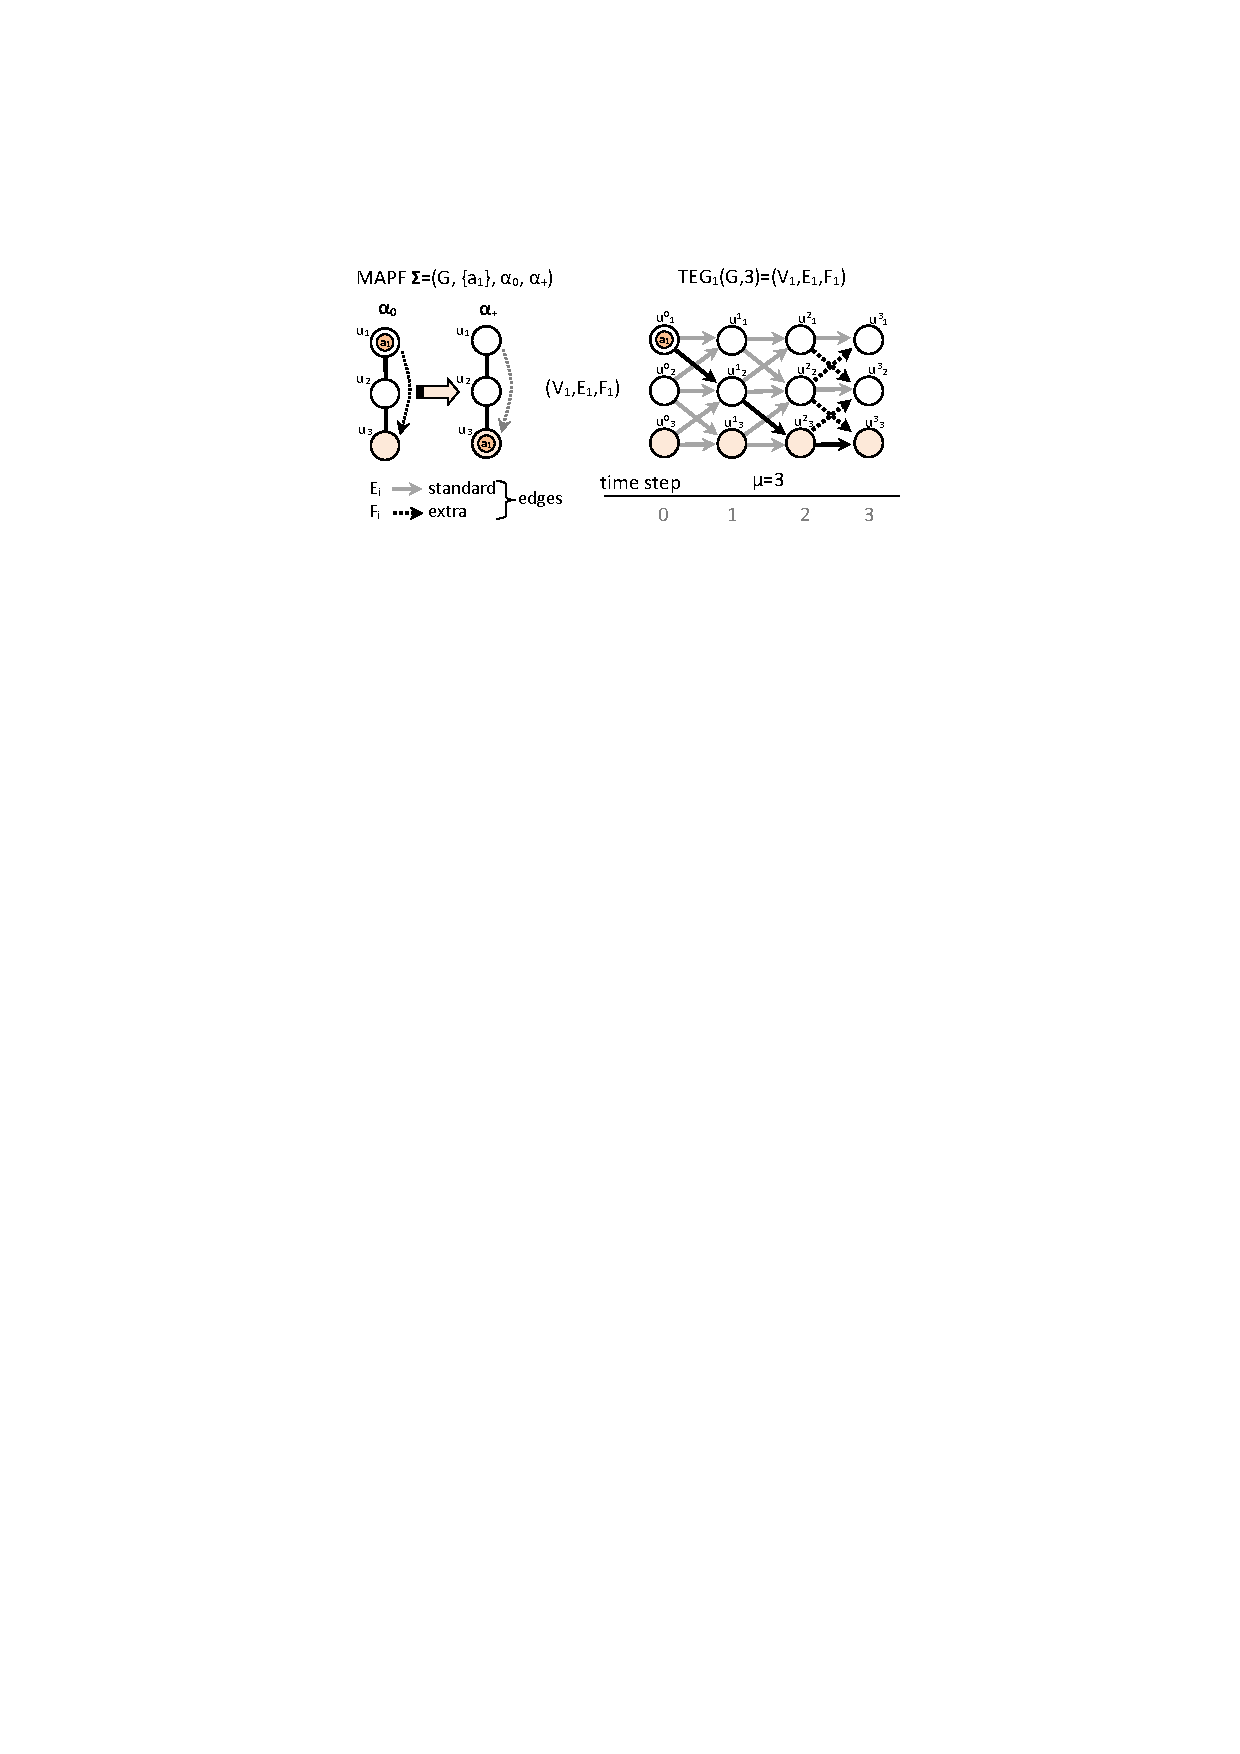
\includegraphics[trim={4.5cm 20.7cm 3.5cm 5.5cm},clip,width=1.0\textwidth]{fig_TEGi.pdf}
\caption{A $TEG_1(3,2)$ for agent $a_1$ that needs to go from $u_1$ to $u_3$.}
\label{figure-TEGi}
\end{figure}

Algorithm~\ref{alg-TEG} lists how to construct the TEG for a given makespan bound $\mu$ and individual cost bound $\xi^i_0$, agent $a_i$, and the underlying graph $G$. 
$TEG_i(\mu,\xi^i_0)=(V_i,E_i,F_i)$ differs from TEG (Definition~\ref{def:TEG}) in that it distinguishes between two types of edges: $E_i$ and $F_i$. $E_i$ are (directed) edges whose destination is at time step $\leq{}\xi^i_0=\xi_0(a_i)$ or represent a wait action in the goal vertex. These are called {\em standard edges}. $F_i$ denoted as \textit{extra edges} are directed edges whose destination is at time step $>{}\xi^i_0=\xi_0(a_i)$ and do not correspond to a wait action in the goal vertex.

Figure~\ref{figure-TEGi} shows an underlying graph for agent $a_1$ (left) and the corresponding $TEG_1(3,2)$. Note that the optimal solution of cost 2 is denoted by the diagonal path in $TEG_1(3,2)$. Edges that belong to $F_i$ are those that their destination is time step 3 and are not corresponding to wait actions (dotted lines). The key in this definition is that the cardinality constraint would only be applied to the extra edges, that is, we will only bound the number of extra edges (they sum up to $\Delta$) making the cardinality constraint more efficient (bounding the number of all edges by $\xi = \xi_0 + \Delta$ is equivalent to bounding the number of extra edges by $\Delta$). The case when agent $a_i$ leaves its goal vertex at time step $t > \xi^i_0$ will be treated separately. In such a case, we need to bound the number of wait actions in the goal vertex between time steps $\xi^i_0$ and $t$, let us call these wait actions {\em non-terminal}.

\subsection{Detailed Description of the SAT Encoding}
\label{sec:detailedDescription}

\noindent Agent $a_i$ must go along a directed path from its initial position to its goal within $TEG_i(\mu,\xi^i_0)$; that is from a vertex in the first layer corresponding to the start position $\alpha_0(a_i)$ to a vertex in the $\mu$-th layer corresponding to the goal position $\alpha_+(a_i)$. The directed path in $TEG_i(\mu,\xi^i_0)$ simulates movement of agent in the underlying graph $G$ (waiting and repeated visits to the same vertex can be modeled).

Hence we need to encode searching for a path from $\alpha_0^0(a_i)$ to $\alpha_+^\mu(a_i)$ in $TEG_i(\mu,\xi^i_0)$ within the Boolean formula. To solve the MAPF problem we need to search for directed paths for individual agents in parallel. Thus possible interactions between agents need to be taken into account to reflect the MAPF movement rules correctly. Additional constraints will be added to capture \textit{collision avoidance} etc. Finally, we will encode the cardinality constraint saying that the number of extra edges and non-terminal wait actions across all TEGs is at most $\Delta$.

We want to ask whether a sum-of-costs solution of $\xi$ exist. For this we build $TEG_i(\mu_0 + \Delta,\xi^i_0)=(V_i,E_i,F_i)$ for each agent $a_i \in A$. Next we introduce the Boolean encoding (denoted \texttt{BASIC-SAT}), formula $\mathcal{F}_{BASIC}(\mu_0, \xi_0, \Delta)$, which has the following Boolean variables:
\vspace{0.25cm}

\noindent {\bf 1:)}  $\mathcal{X}^t_j(a_i)$ for every $t \in \{0,1,...,\mu \}$
and $u^t_j \in V_i$ -- Boolean variable of whether agent $a_i$ is in vertex $u_j$ at time step $t$.
\vspace{0.25cm}

\noindent {\bf 2:)} $\mathcal{E}^t_{j,k}(a_i)$ for every $t \in \{0,1,...,\mu-1
\}$ and $(u^t_j,u^{t+1}_l) \in (E_i \cup F_i)$ -- Boolean variables that model transition of agent $a_i$ from vertex $u_j$ to vertex $u_l$ through any edge (standard or extra) between time steps $t$ and $t+1$ respectively.
\vspace{0.25cm}

\noindent {\bf 3:)}  $\mathcal{C}^t(a_i)$ for every $t \in \{0,1,...,\mu-1 \}$ such that there exist $u^t_j \in V_i$ and $u^{t+1}_l \in V_i$ with $(u^t_j,u^{t+1}_l) \in F_i$ --- Boolean variables that model cost of movements along {\bf extra edges} (from $F_i$) between time steps $t$ and $t + 1$. We denote by $\mathcal{C}$ the set of all such variables. 
\vspace{0.25cm}

We now introduce constraints on these variables to restrict illegal values as
defined by our variant of MAPF. Other variants may use a slightly different
encoding but the principle is the same. Let $T_\mu = \{0, 1, ..., \mu-1\}$.
Several groups of constraints are introduced for each agent $a_i \in A$ as
follows:
\vspace{0.25cm}

\noindent{\bf C1:} If an agent appears in a vertex at a given time step, then it must follow through exactly one adjacent edge into a vertex in the next time step. This is encoded by the following two constraints, which are posted for every $t \in T_\mu$ and $u^t_j \in V_i$

\begin{equation}
   {  \mathcal{X}^t_j(a_i) \Rightarrow \bigvee_{(u^t_j,u^{t+1}_l) \in E_i \cup F_i }{\mathcal{E}^t_{j,l}(a_i),}
      }\label{eq:basic-start}
\end{equation}

\begin{equation}
   {  \sum_{(u^t_j,u^{t+1}_l) \in E_i \cup F_i }{\mathcal{E}^t_{j,l}(a_i)} \leq 1
      }
            \label{eq:basic-2}
\end{equation}
\vspace{0.25cm}

The pseudo-Boolean constraint (\ref{eq:basic-2}) (often called {\em at-most-one} constraint) can be translated to clauses in multiple different ways \cite{DBLP:conf/cp/AnsoteguiBCDEMN19}. One simple and efficient translation at the same time is to forbid all possible pairs variables to be simultaneously $\mathit{TRUE}$ as follows. As the translation consists of binary clauses only it supports {\em unit propagation} \cite{DBLP:journals/jlp/DowlingG84} inside the SAT solver.

\begin{equation}
   {  \bigwedge_{(u^t_j,u^{t+1}_{l}),(u^t_j,u^{t+1}_{l'}) \in E_i \cup F_i \wedge l<l'}{\neg\mathcal{E}^t_{j,{l}}(a_i) \vee \neg\mathcal{E}^t_{j,{l'}}(a_i)}
      }
            \label{eq:basic-3}
\end{equation}
\vspace{0.25cm}

\noindent{\bf C2:} Whenever an agent occupies an edge it must also enter it before and leave it at the next time-step. This is ensured by the following constraint introduced for every $t \in T_\mu$ and $(u^t_j,u^{t+1}_l) \in E_i \cup F_i$:
\begin{equation}
   {  \mathcal{E}^t_{j,l}(a_i) \Rightarrow \mathcal{X}^t_j(a_i) \wedge \mathcal{X}^{t+1}_l(a_i)
    } \label{eq:basic-4}
\end{equation}
\vspace{0.25cm}

\noindent{\bf C3:} The target vertex of any movement except a wait action must be empty. This is ensured by the following constraint introduced for every $t \in T_\mu$ and $(u^t_j,u^{t+1}_l) \in E_i \cup F_i$ such that $j \neq l$.
\begin{equation}
   {  \mathcal{E}^t_{j,l}(a_{i}) \Rightarrow \bigwedge_{a_{i'} \in A \wedge {i'} \neq i \wedge u^t_j \in V_{i'}}{\neg \mathcal{X}^t_j(a_{i'})}
    } \label{eq:basic-5}
\end{equation}
\vspace{0.25cm}

\noindent{\bf C4:} No two agents can appear in the same vertex at the same time step. That is the following constraint is added for every $t \in T_\mu$ and vertex $u^t_j \in V^t$:

\begin{equation}
   {  \sum_{u^t_j \in V_i}{\mathcal{X}^t_j(a_i)} \leq 1
    }\label{eq:basic-6}
\end{equation}

Again this pseudo-Boolean at-most-one constraint can be translated to clauses by forbidding any pair of agents $a_i,a_{i'} \in A$ such that $i < {i'}$ to appear simultaneously in a vertex:

\begin{equation}
   {  \bigwedge_{u^t_j \in V_i\cap V_{i'}}{\neg \mathcal{X}^t_j(a_i) \vee \neg \mathcal{X}^t_j(a_{i'})}
    }\label{eq:basic-7}
\end{equation}
\vspace{0.25cm}

\noindent{\bf C5:} Whenever an extra edge is traversed the cost needs to be accumulated. In fact, this is the cost that we accumulate as discussed above. This is done by the following constraint for every $t \in T_\mu$ and extra edge $(u^t_j,u^{t+1}_l) \in F_i$.
\begin{equation}
   { \mathcal{E}^t_{j,l}(a_i) \Rightarrow \mathcal{C}^t(a_i)
    }\label{eq:basic-8}
\end{equation}
\vspace{0.25cm}

%Variables and clauses introduced so far correspond to time expansion generated
%by \textsf{Encode-Time-Expansion} which gets collection of TEGs for each agent
%as a parameter.
%Next, we will want the number  of $\mathcal{C}^t(a_i)$ variables that are
%$TRUE$ to be $\leq \Delta$.

%\begin{itemize}
%    \item {The cost of wait action followed by a not wait action need to be accumulated. This is ensured by the following constraint for every $t \in \{0, 1, ...,\mu-1\}$.  }
%\begin{equation}
%   { \mathcal{C}^t(a_i) \Rightarrow \bigwedge_{\sigma \in \{1,2,...,t-1 \} \wedge \{(u^\sigma_j,u^{\sigma+1}_k) \in F_i\} \neq \emptyset }\mathcal{C}^\sigma(a_i)
%    }
%\end{equation}
%\end{itemize}

\noindent{\bf C6:} If agent $a_i$ leaves the goal all wait actions before leaving the goal must be accumulated to the cost. These actions correspond to non-terminal wait actions. Hence the following constraint is added for each agent $a_i$ and  $t \in T_\mu$:
\begin{equation}
   { \mathcal{C}^t(a_i) \Rightarrow \bigwedge_{t' \in \{\xi_i^0,\xi_i^0+1,...,t-1\}}{\mathcal{C}^{t'}(a_i)}
    }\label{eq:basic-9}
\end{equation}
\vspace{0.25cm}


\noindent{\bf C7: Cardinality constraint.} Finally the bound on the total cost needs to be introduced. Reaching the sum-of-costs of $\xi$ corresponds to traversing exactly $\Delta$ extra edges from $F_i$ or non-terminal wait actions. This corresponds to the following simple cardinality constraint over the variables in $\mathcal{C}$:
\begin{equation}
  \leq_{\Delta} \{ C\in \mathcal{C} \} 
        \label{eq:basic-end}
\end{equation}
\vspace{0.25cm}

% \begin{equation}
%   { \leq_{\Delta}\big\{\;
%   \mathcal{C}^t(a_i)\;|\;i=1,2,...,m; t=0,1,...,{\mu-1} \wedge \{(u^t_j,u^{t+1}_k) \in F_i\} \neq \emptyset
%   \;\big\}
%     }
%     % the notation with \leq with no left hand side is a standard notation for cardinality constraints
%         \label{eq:basic-end}
% \end{equation}
% The right most part of this condition ($\{(u^_j, u^{t+1}_k)\in F_i\}\neq 0$)....


\noindent{\bf Final formula.}  The resulting Boolean formula $\mathcal{F}_{BASIC}(\mu_0, \xi_0, \Delta)$ is a
conjunction of $C1, C2,$ $\ldots C7$ and is the one that is constructed and consulted by Algorithm~\ref{alg-MAPF-SAT-soc} (lines 11 and 12).
\vspace{0.25cm}

The constraints also imply that agent cannot swap their positions, that is for example two agents moving in opposite directions in a corridor to cross each other and move on is forbidden. The following propositions summarize the correctness and the space complexity of our \texttt{BASIC-SAT} encoding.

\begin{proposition}
MAPF $\Sigma=({G=(V,E)},A,\alpha_0,\alpha_+)$ has a \textit{sum-of-costs} solution of $\xi$ if and only if $\mathcal{F}_{BASIC}(\mu, \Delta)$ is satisfiable. Moreover, a solution of MAPF $\Sigma$ with the sum-of-costs of $\xi$ can be extracted from the satisfying assignment of $\mathcal{F}_{BASIC}(\mu_0, \xi_0, \Delta)$ by interpreting its $\mathcal{X}^t_j(a_i)$ variables.
\end{proposition}


\noindent {\bf Proof:} The direct consequence of the above definitions is that a valid solution of a given MAPF $\Sigma$ of sum-of-costs $\xi$ corresponds to non-conflicting directed paths in the TEGs of the individual agents that in total use at most $\Delta$ extra edges and non-terminal wait actions. These non-conflicting paths further correspond to variable assignment satisfying $\mathcal{F}_{BASIC}(\mu_0, \xi_0, \Delta)$, i.e., variable assignments represent directed paths in TEGs plus they satisfy bounds imposed by the cardinality constraint. $_\Box$

\begin{proposition}
Let $D$ be the maximal degree of any vertex in $G$ and let $k$ be the number of agents. If $k \cdot|E|\geq \Delta = \xi-\xi_0$ and $k \geq D$ then the number of clauses in $\mathcal{F}_{BASIC}(\mu_0,\xi_0, \Delta)$ is $\mathcal{O}(\mu \cdot k^2\cdot |E|)$, and the number of variables is $\mathcal{O}(\mu \cdot k \cdot |E|)$
 \end{proposition}
 
\noindent {\bf Proof:} The components of $\mathcal{F}_{BASIC}(\mu_0,\xi_0, \Delta)$ are described in equations~ (\ref{eq:basic-start}) -- (\ref{eq:basic-end}). Equation~(\ref{eq:basic-start}) introduces at most $\mathcal{O}(k\cdot \mu \cdot |E| )$ clauses. Equation~(\ref{eq:basic-3}) introduces at most $\mathcal{O}(k\cdot \mu |E| \cdot D)$ clauses. Equation~(\ref{eq:basic-4}) introduces at most $\mathcal{O}(k \cdot \mu \cdot |E|)$ clauses. Equation~(\ref{eq:basic-5}) introduces at most $\mathcal{O}(k^2\cdot \mu \cdot |E|)$.
Equation~(\ref{eq:basic-7}) introduces at most $\mathcal{O}(k^2\cdot \mu \cdot |V|)$ clauses. Equation~(\ref{eq:basic-8}) introduces at most $\mathcal{O}(k\cdot \mu \cdot |E|)$ clauses. Equation ~(\ref{eq:basic-9}) introduces at most $\mathcal{O}(k \cdot \mu \cdot (\xi-\xi_0))$ binary clauses since each implication from (\ref{eq:basic-9}) develops into at most $\xi-\xi_0$ binary clauses. Equation~(\ref{eq:basic-end}) introduces at most $\mathcal{O}(k\cdot \mu \cdot (\xi-\xi_0))$ clauses, since the constraint checking that $m$ variables has a cardinality constraint of $\lambda$ requires $\mathcal{O}(m\cdot \lambda)$ clauses~\cite{DBLP:conf/cp/Sinz05}. Summing all the above results in a total of $\mathcal{O}(\mu \cdot k\cdot (|E| \cdot (D+k) + (\xi-\xi_0)))$. If we assume that $k>D$ and that $k \cdot|E|> (\xi-\xi_0)$ then the number of clauses is $\mathcal{O}(\mu \cdot k^2\cdot |E|)$. The number of variables is computed in a similar way. $_\Box$


\subsection{Improving Basic SAT by Adding MDDs}

\noindent The major parameter that affects the speed of solving of Boolean formulae is their size \cite{DBLP:books/sp/Petke15}. The size of formulae in the BASIC-SAT encoding is affected mostly by the size of the TEGs (this is embodied in the $|V|$ and $|E|$ factors in the encoding size). To obtain a significant speedup we reduce the size of $TEG_i$ for agent $a_i$ in terms of the number of vertices while the soundness of encoding is preserved. To do this we borrow the ideas of {\em Multi-Value Decision Diagram} (MDD) \cite{DBLP:conf/cp/AndersenHHT07} from the search-based MAPF algorithm \textsc{Icts} \cite{DBLP:journals/ai/SharonSGF13}. This shows the advantage of combining techniques from both classes of approaches (search-based and SAT).

\begin{figure}[h]
\centering
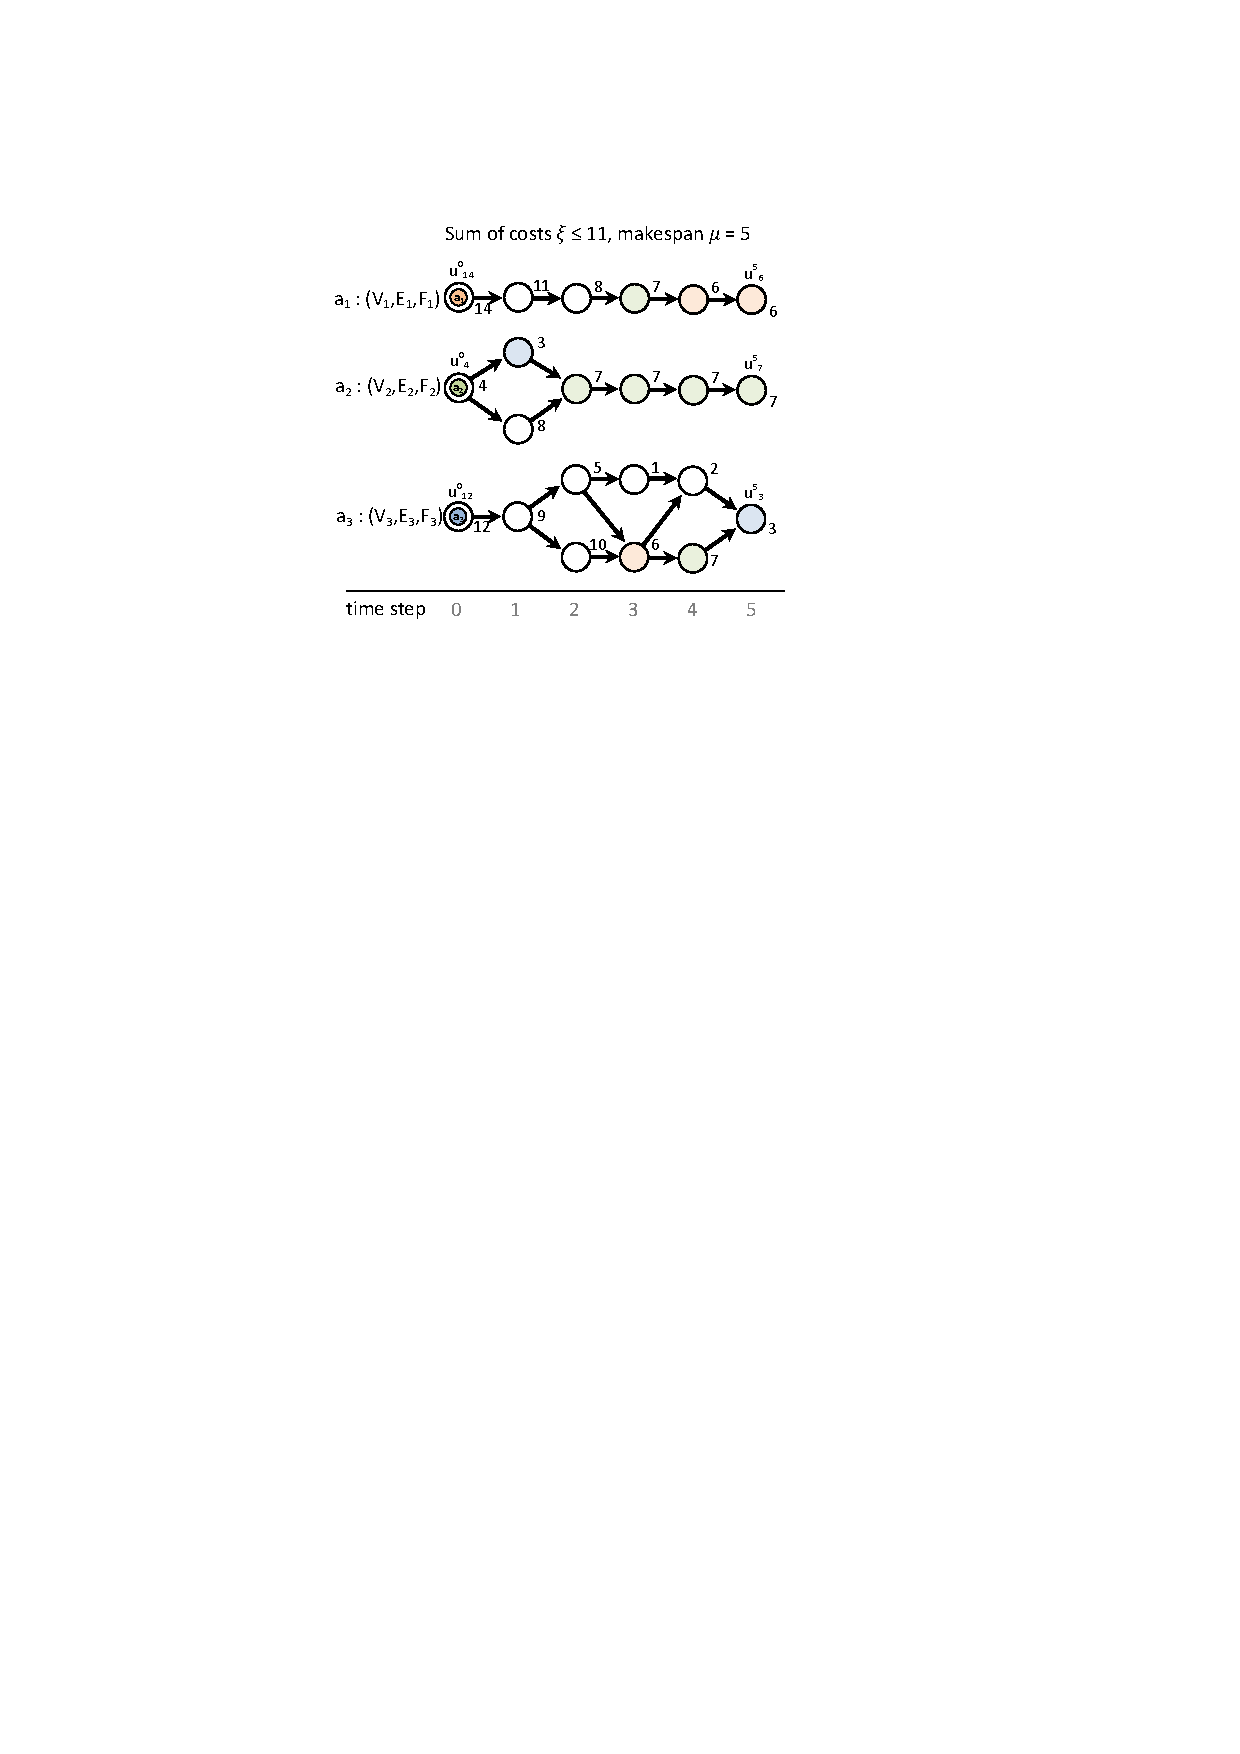
\includegraphics[trim={2.5cm 19cm 4cm 2.5cm},clip,width=1.0\textwidth]{fig_MDD.pdf}
\caption{MDDs for agents $a_1$, $a_2$, and $a_3$ for the MAPF from Figure
\ref{figure-MAPF} for \textit{sum of individual cost} $\xi\leq 11$. Specifically, $MDD_1(5,4)$, $MDD_2(5,2)$, and $MDD_3(5,5)$ are shown (no extra edges are present). }
\label{figure-MDD}
\end{figure}

Let $TEG_{i}(\mu,\xi^i_0)$ denote $TEG_i$ for $\mu$ time expansions where $\mu=\mu_0+\Delta$. $MDD_i(\mu,\xi^i_0)$ is a digraph that represents all possible valid paths from $\alpha_0(a_i)$ to $\alpha_+(a_i)$ of makespan/cost $\mu$ for agent $a_i$ (in the case of single agent the makespan and the sum-of-costs are the same). $MDD_i(\mu,\xi^i_0)$ has a single {\em source node} at level 0 and a single {\em sink node} at level $\mu$. Every node at depth $t$ of $MDD_i^\mu$ corresponds to a possible position of $a_i$ at time $t$, that is a position on a path of cost $\mu$ from $\alpha_0(a_i)$ to $\alpha_+(a_i)$. In other words, vertex $u_j \in V$ that is too far from either $\alpha_0(a_i)$ or $\alpha_+(a_i)$ is not represented in $MDD_i(\mu,\xi^i_0)$. If there is no path of makespan/cost $\mu$ from $\alpha_0(a_i)$ to $\alpha_+(a_i)$ containing $u_j$, then $u_j$ is not included in $MDD_i(\mu,\xi^i_0)$. Similarly as in $TEG_i(\mu,\xi^i_0)$, the parameter $\xi^i_0$ is used to distinguish between the standard edges (those that terminate in time step $\leq \xi^i_0$ or represent the wait action in the goal vertex) in MDD and extra edges (those that terminate at time step $> \xi^i_0$ and do not correspond to the wait action in the goal vertex).

\begin{figure}[h]
\centering
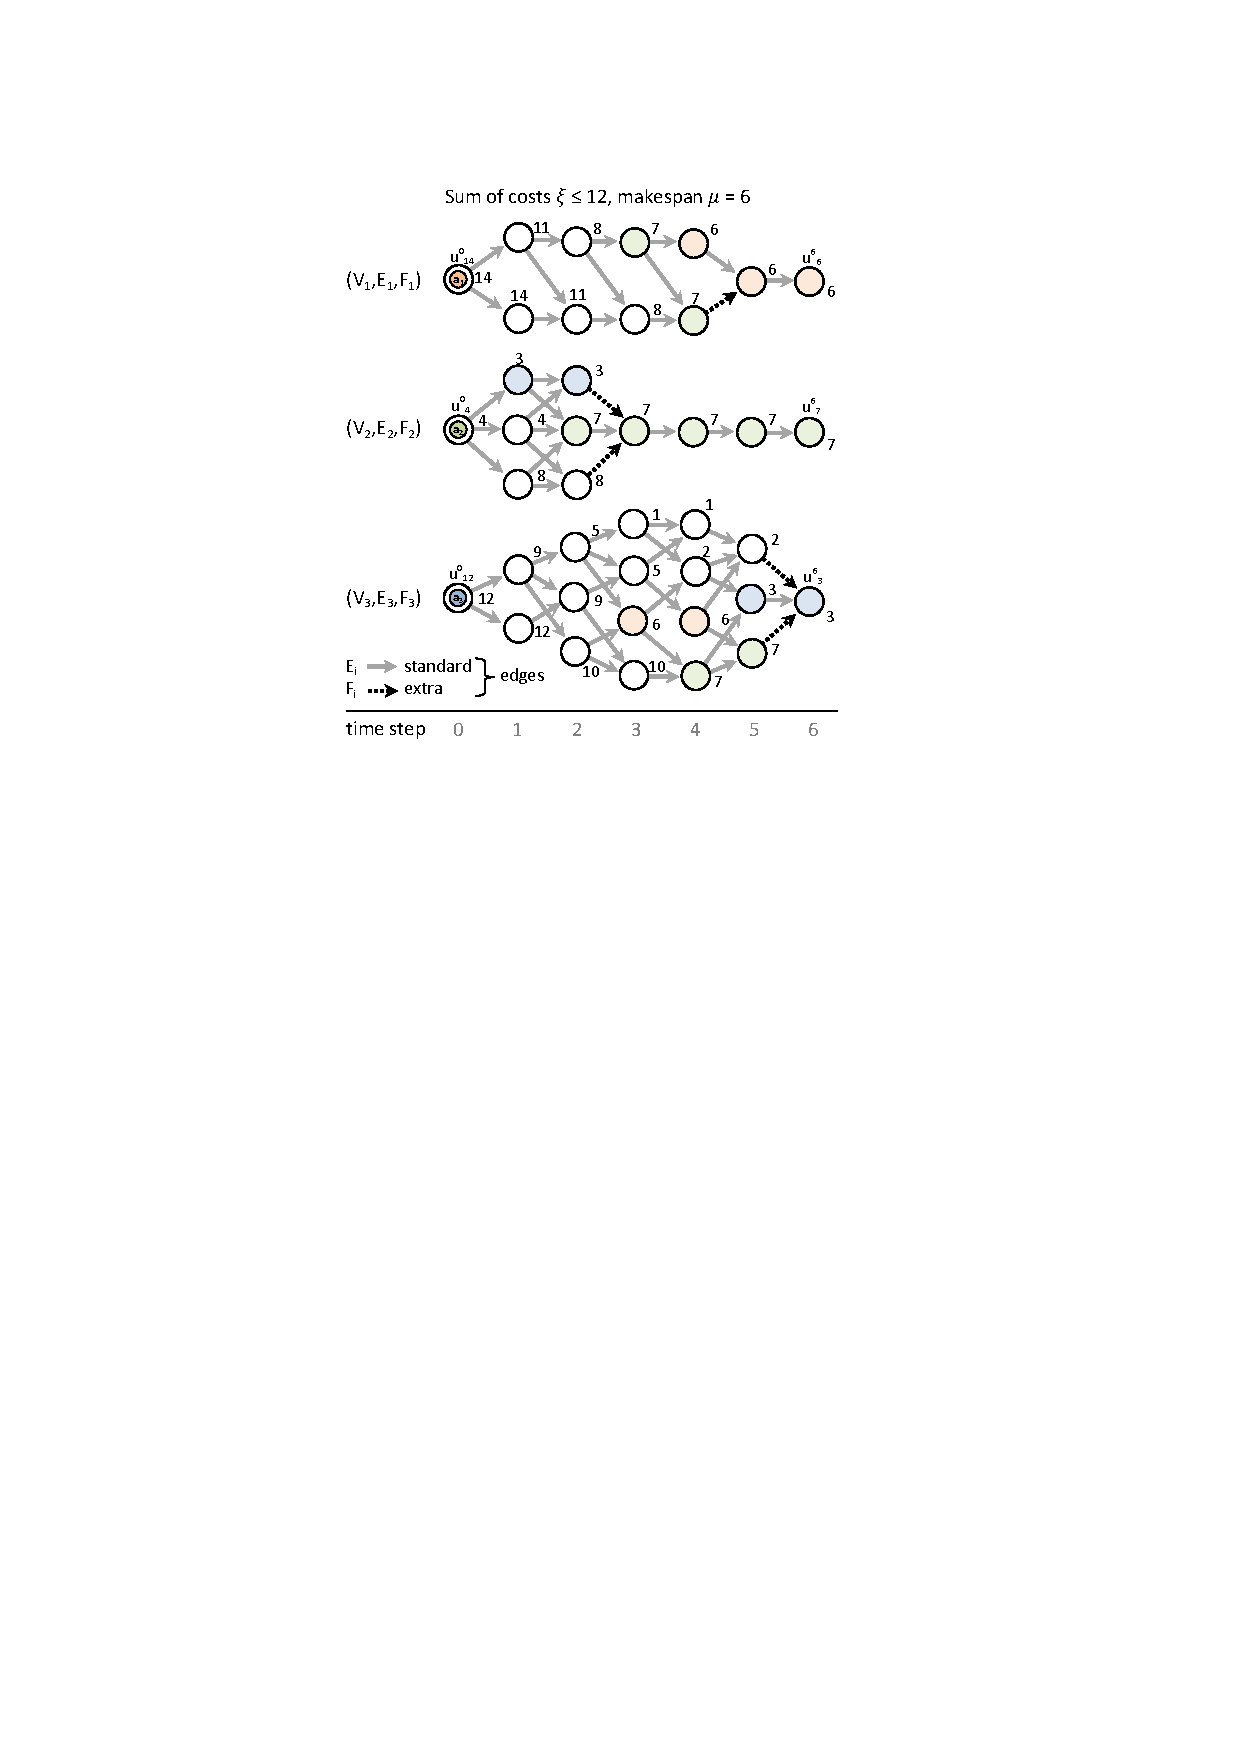
\includegraphics[trim={3.5cm 17.2cm 3.5cm 3.1cm},clip,width=1.0\textwidth]{fig_MDDplus.pdf}
\caption{MDDs from Figure \ref{figure-MDD} for the incremented \textit{individual cost} from 11 to 12 ($\xi\leq 12$).}
\label{figure-MDDplus}
\end{figure}

It is easy to see that $MDD_i(\mu, \xi^i_0)$ is a subgraph of $TEG_i(\mu,\xi^i_0)$. While $TEG_i(\mu,\xi^i_0)$ includes all vertices of $G$ at each time step, $MDD_i(\mu,\xi^i_0)$ includes only those vertices and edges that are reachable within makespan/cost $\mu$, and thus vertices not in $MDD_i(\mu,\xi^i_0)$ can be ignored.


Moreover, the maximum cost that can be consumed by single agent $a_i$ under given sum-of-costs bound $\xi=\xi_0 + \Delta$ is $\xi_0(a_i) + \Delta$ where, as defined above, $\xi_0(a_i)$ is the length of the shortest path connecting $\alpha_0(a_i)$ with $\alpha_+(a_i)$ in $G$ (assuming no other agent exists). Thus, it is sufficient to replace $TEG_i(\mu_0+\Delta,\xi^i_0)$ with $MDD_i(\mu_0+\Delta,\xi^i_0)$ in the algorithm.

%which is useful since $\xi_0(a_i)+\Delta \leq \mu_0+\Delta = \mu$.

MDDs for the agents of Figure~\ref{figure-MAPF} are shown in Figures \ref{figure-MDD} and \ref{figure-MDDplus}. Indeed, the size of the MDDs is much smaller than the corresponding TEGs, which include all states for all time steps. Though the increase in size caused by ability to reach more vertices under given the next  sum-of-costs bounds is observable between Figures \ref{figure-MDD} and \ref{figure-MDDplus}.

\begin{figure}[h]
\centering
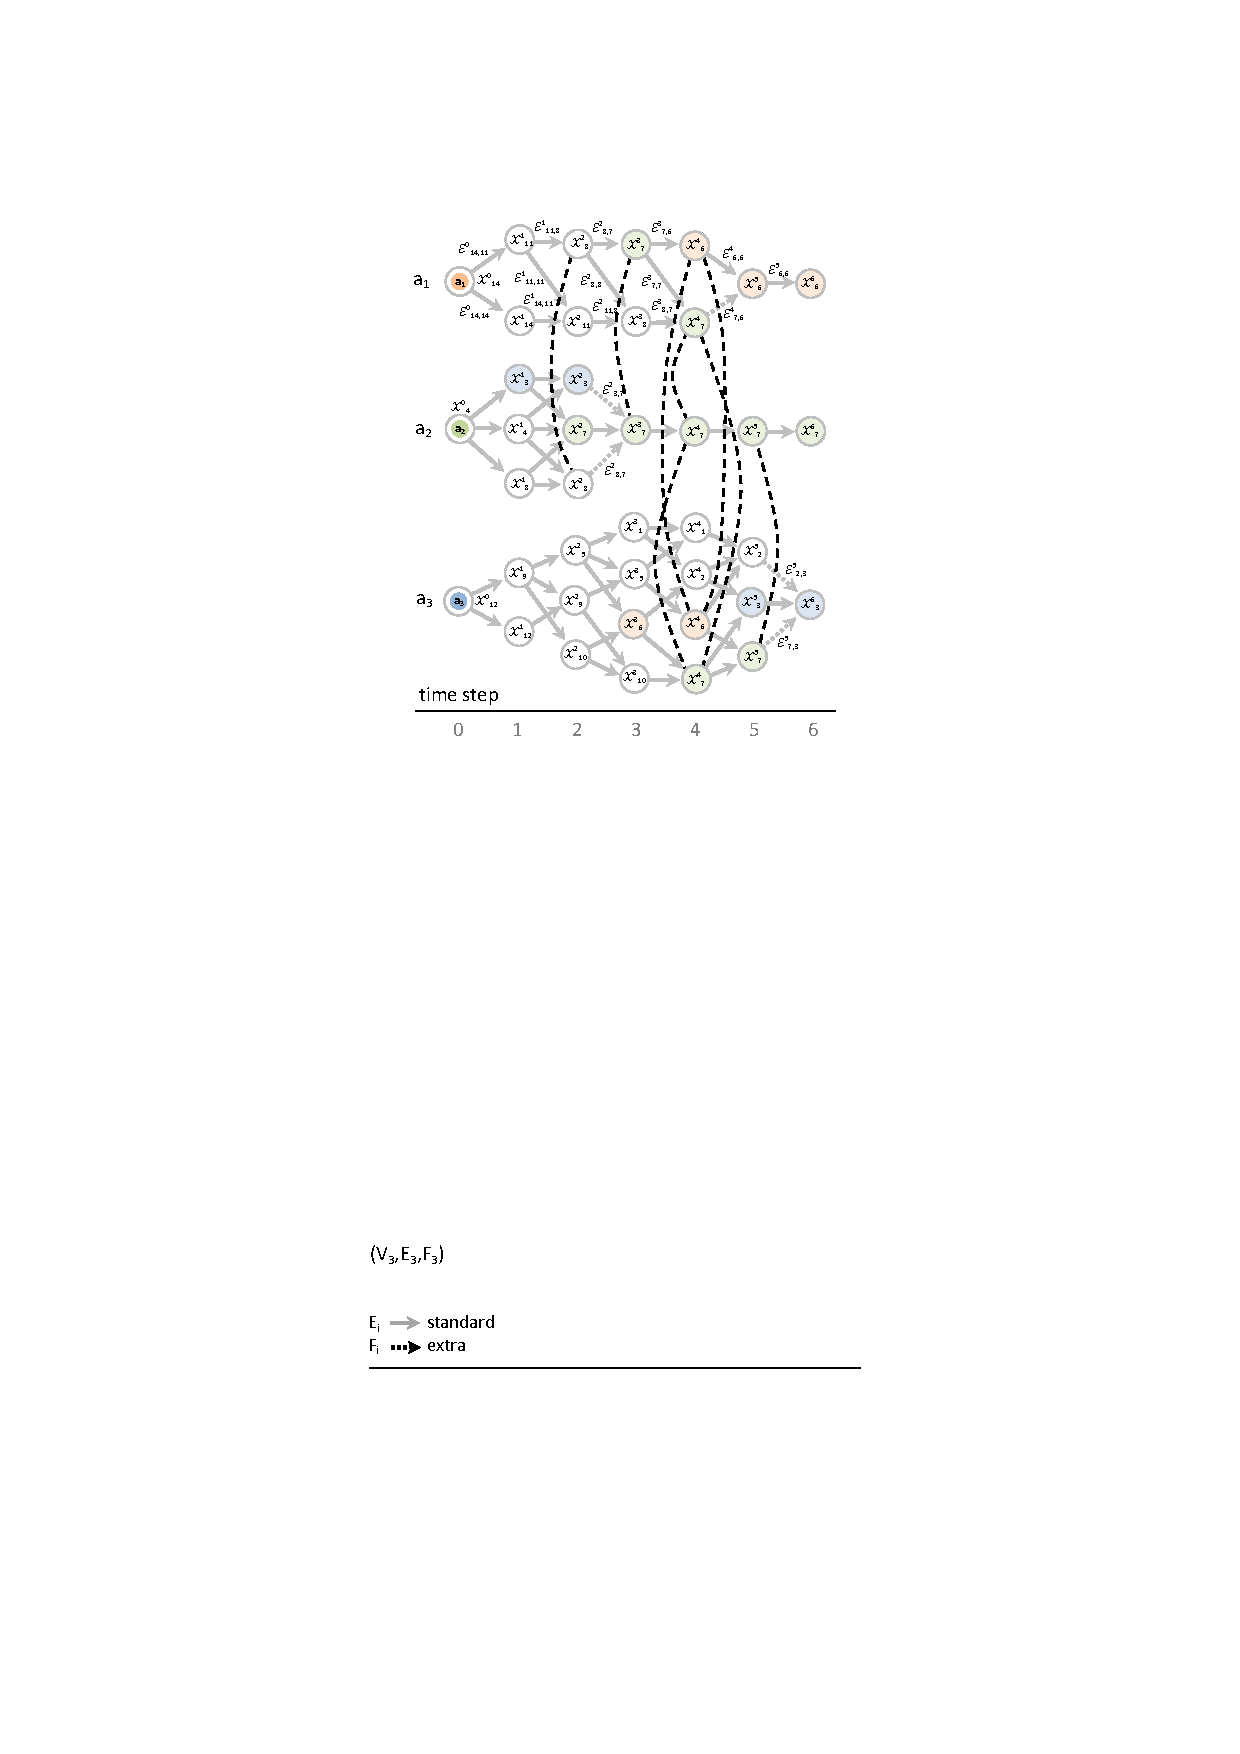
\includegraphics[trim={3.5cm 17.2cm 3.5cm 3.7cm},clip,width=1.0\textwidth]{fig_MDDencoding.pdf}
\caption{An illustration of MDD-SAT encoding using MDDs from Figure \ref{figure-MDDplus}. Mutual exclusion constraints (C4) that prevent multiple agent occurrence in the same vertex are shown using dashed edges.}
\label{figure-MDDencoding}
\end{figure}

The encoding that uses MDD-based time expansion will be called MDD-SAT and the corresponding formulae will be denoted as $\mathcal{F}_{MDD}(\mu_0, \xi_0, \Delta)$. The formula is similar to the BASIC-SAT encoding. The only difference is that in BASIC-SAT there is a variable for all vertices and edges of the TEGs while in MDD-SAT, only variables for the vertices and edges of the MDDs are needed. This difference can be significant. Table~\ref{table_size_8x8} presents the number of Boolean variables and clauses accumulated over all the constructed formulae for a given MAPF instance for BASIC-SAT and for MDD-SAT over $8 \times 8$ grid with 10\% obstacles. The average values out of 10 random instances per number of agents are shown. Up to two orders of magnitude reduction can be observed when MDDs are used.

An illustration of the $\mathcal{F}_{MDD}(\mu_0,\xi_0,\Delta)$ formula is shown in Figure \ref{figure-MDDencoding}. It is particularly observable that MDDs reduce the number of mutual exclusion ({\em mutex}) constraints (dashed edges) by omitting unreachable vertices (and all the constraints incident with them).


\begin{table}
\centering
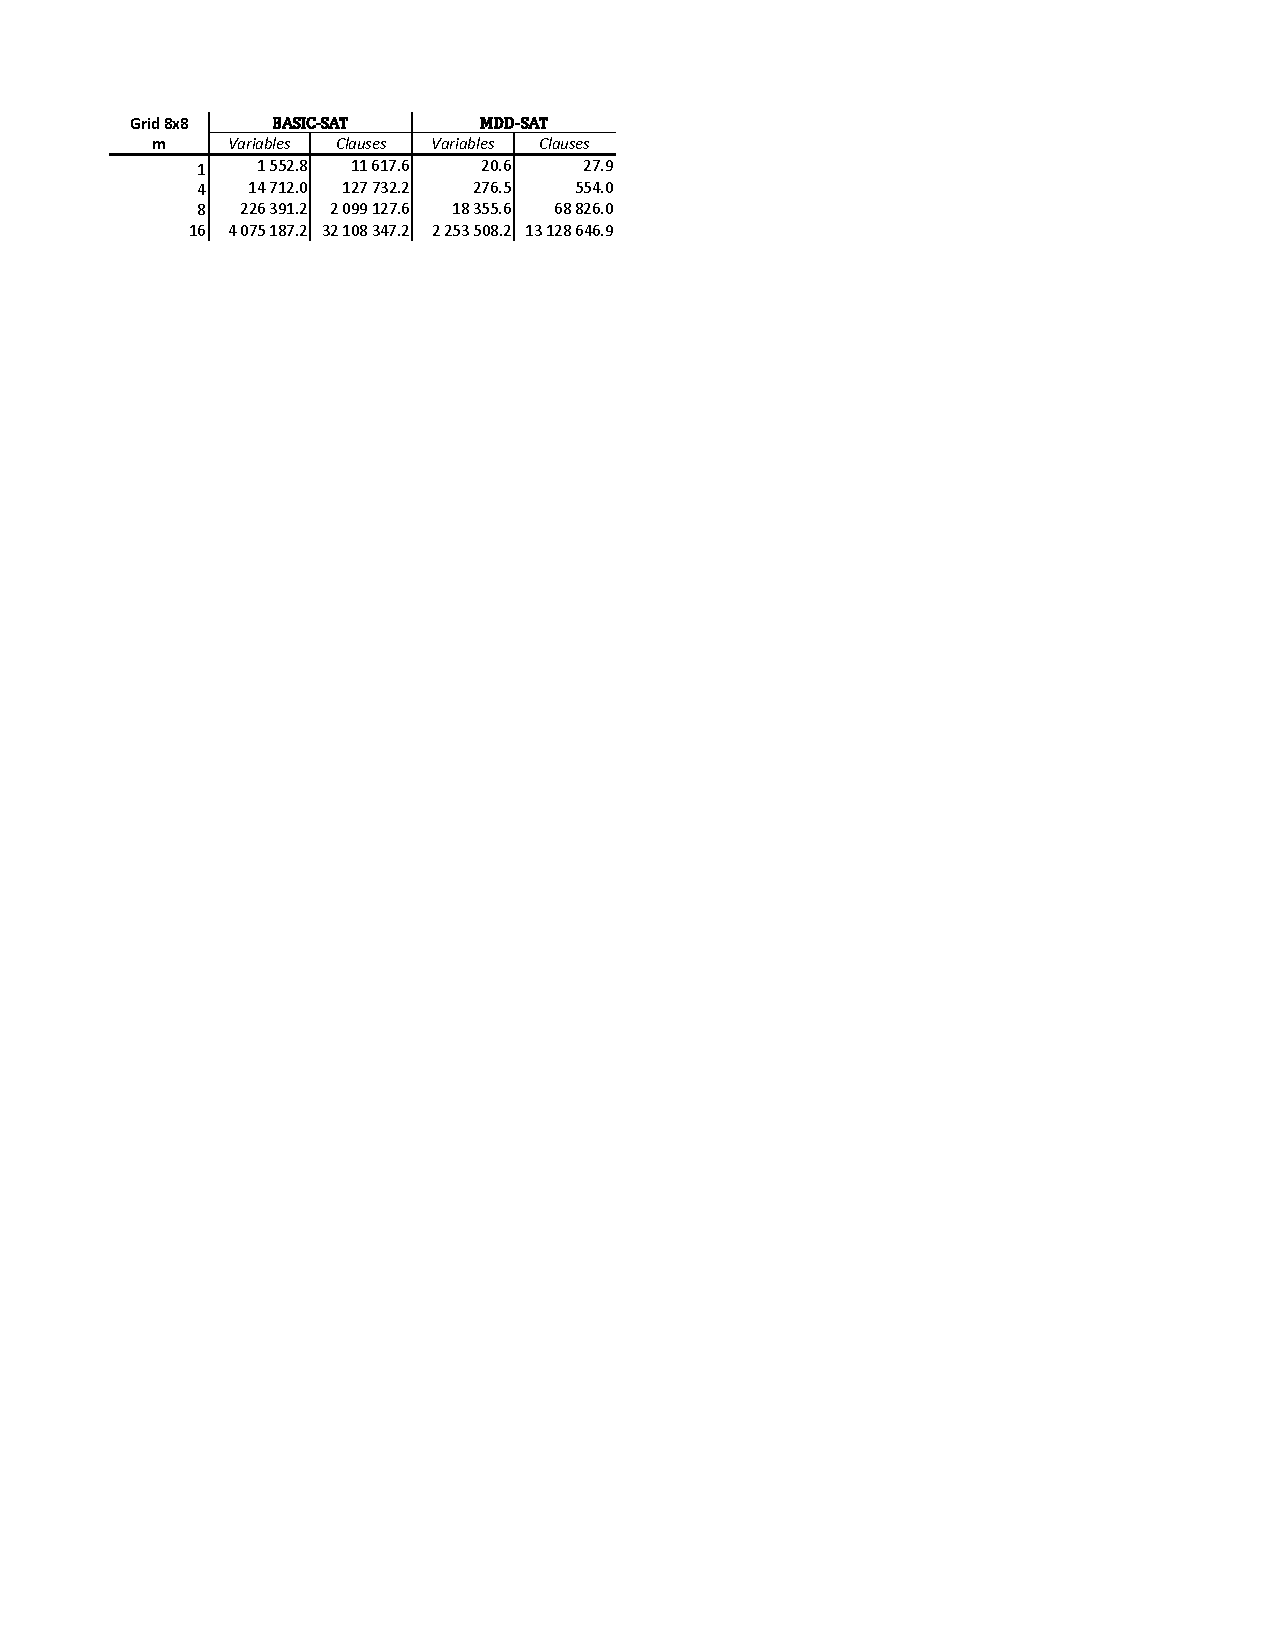
\includegraphics[trim={2cm 23.9cm 11cm 1.9cm},clip,width=0.75\textwidth]{table_size_8x8.pdf}
\caption{The effect of using MDDs in the encoding in terms of the number of variables and clauses.} \label{table_size_8x8}
\end{table}


\section{Experimental Results for MDD-SAT}

We experimented on 4-connected grids with randomly placed obstacles \cite{DBLP:conf/aiide/Silver05} and on \textit{Dragon Age} maps \cite{CBSJUR,sturtevant2012benchmarks}. Both settings are a standard MAPF benchmarks. The initial position of the agents was randomly selected. To ensure solvability the goal positions were selected by performing a long \textit{random walk} from the initial configurations.

% Which algorithms we evaluated

We compared our SAT solvers to several state-of-the-art search-based algorithms: the \textit{increasing cost tree search} - \textsc{Icts}
\cite{DBLP:journals/ai/SharonSGF13}, {\em Enhanced Partial Expansion A*} - \textsc{Epea}* \cite{EPEJAIR} and \textit{improved conflict-based search} - \textsc{Icbs} \cite{DBLP:conf/ijcai/BoyarskiFSSTBS15}.  For all the search algorithms we used the best known setup of their parameters and enhancements suitable for solving the given instances over 4-connected grids.

The SAT approaches were implemented in C++ \footnote{The implementation is available as part of a MAPF experimental project on: https://github.com/surynek/reLOC.}. The implementation consists of a top level algorithm for finding the optimal sum-of-costs $\xi$ and {\em CNF} formula generator \cite{Biere:2009:HSV:1550723} that prepares input formula for a SAT solver into a file. The SAT solver is an external module our this architecture. We used \texttt{Glucose 3.0} \cite{DBLP:conf/ijcai/AudemardS09,DBLP:conf/sat/AudemardLS13}, which is a top-performing SAT solver in the recent editions of the \textit{SAT Competition} \cite{DBLP:journals/aim/JarvisaloBRS12,DBLP:conf/ictai/Surynek14,DBLP:conf/aaai/BalyoHJ17}.
% For reviewer
Since the SAT solver is called multiple times when solving a single MAPF problem, we call it directly through its API. This SAT solver also supports incremental SAT solving~\cite{fazekas2019incremental,DBLP:conf/sat/AudemardLS13}, that is, it is possible to add variables and clauses incrementally between calls, and the solver is able utilize this to learn clauses and speedup its search.

The cardinality constraint was encoded using the standard circuit based encoding called \textit{sequential counter} \cite{DBLP:conf/cp/Sinz05}. In our initial testing we considered various encodings of the cardinality constraint \cite{DBLP:conf/cp/BailleuxB03,DBLP:conf/cp/SilvaL07}. Our finding is that changing the encoding has a minor effect \footnote{Due to the knowledge of lower bounds on the sum-of-costs, the number of variables involved in the cardinality constraint is relatively small and hence the different encoding style has not enough room to show its benefit.}

\textsc{Icts} and \textsc{Icbs} were implemented in C\#, based on their original implementation (here we used a slight modification in which the target vertex of a move must be empty). All experiments were performed on a system with Xeon 2.8Ghz core with 32 Gb of memory.

\subsection{Square Grid Experiments}

We first experimented on  $8{}\times{}8$, $16{}\times{}16$, and $32{}\times{}32$ grids with 10\% obstacles while increasing the number of agents from 1 up to the last number where at least one solver was able to solve an instance with that number of agents (in case of the $8{}\times{}8$ grid this is 17 agents; and 32 and 60 in case of $16{}\times{}16$ and $32{}\times{}32$ grids respectively). For each number of agents 10 random instances were generated.

\begin{figure}[t]
\centering
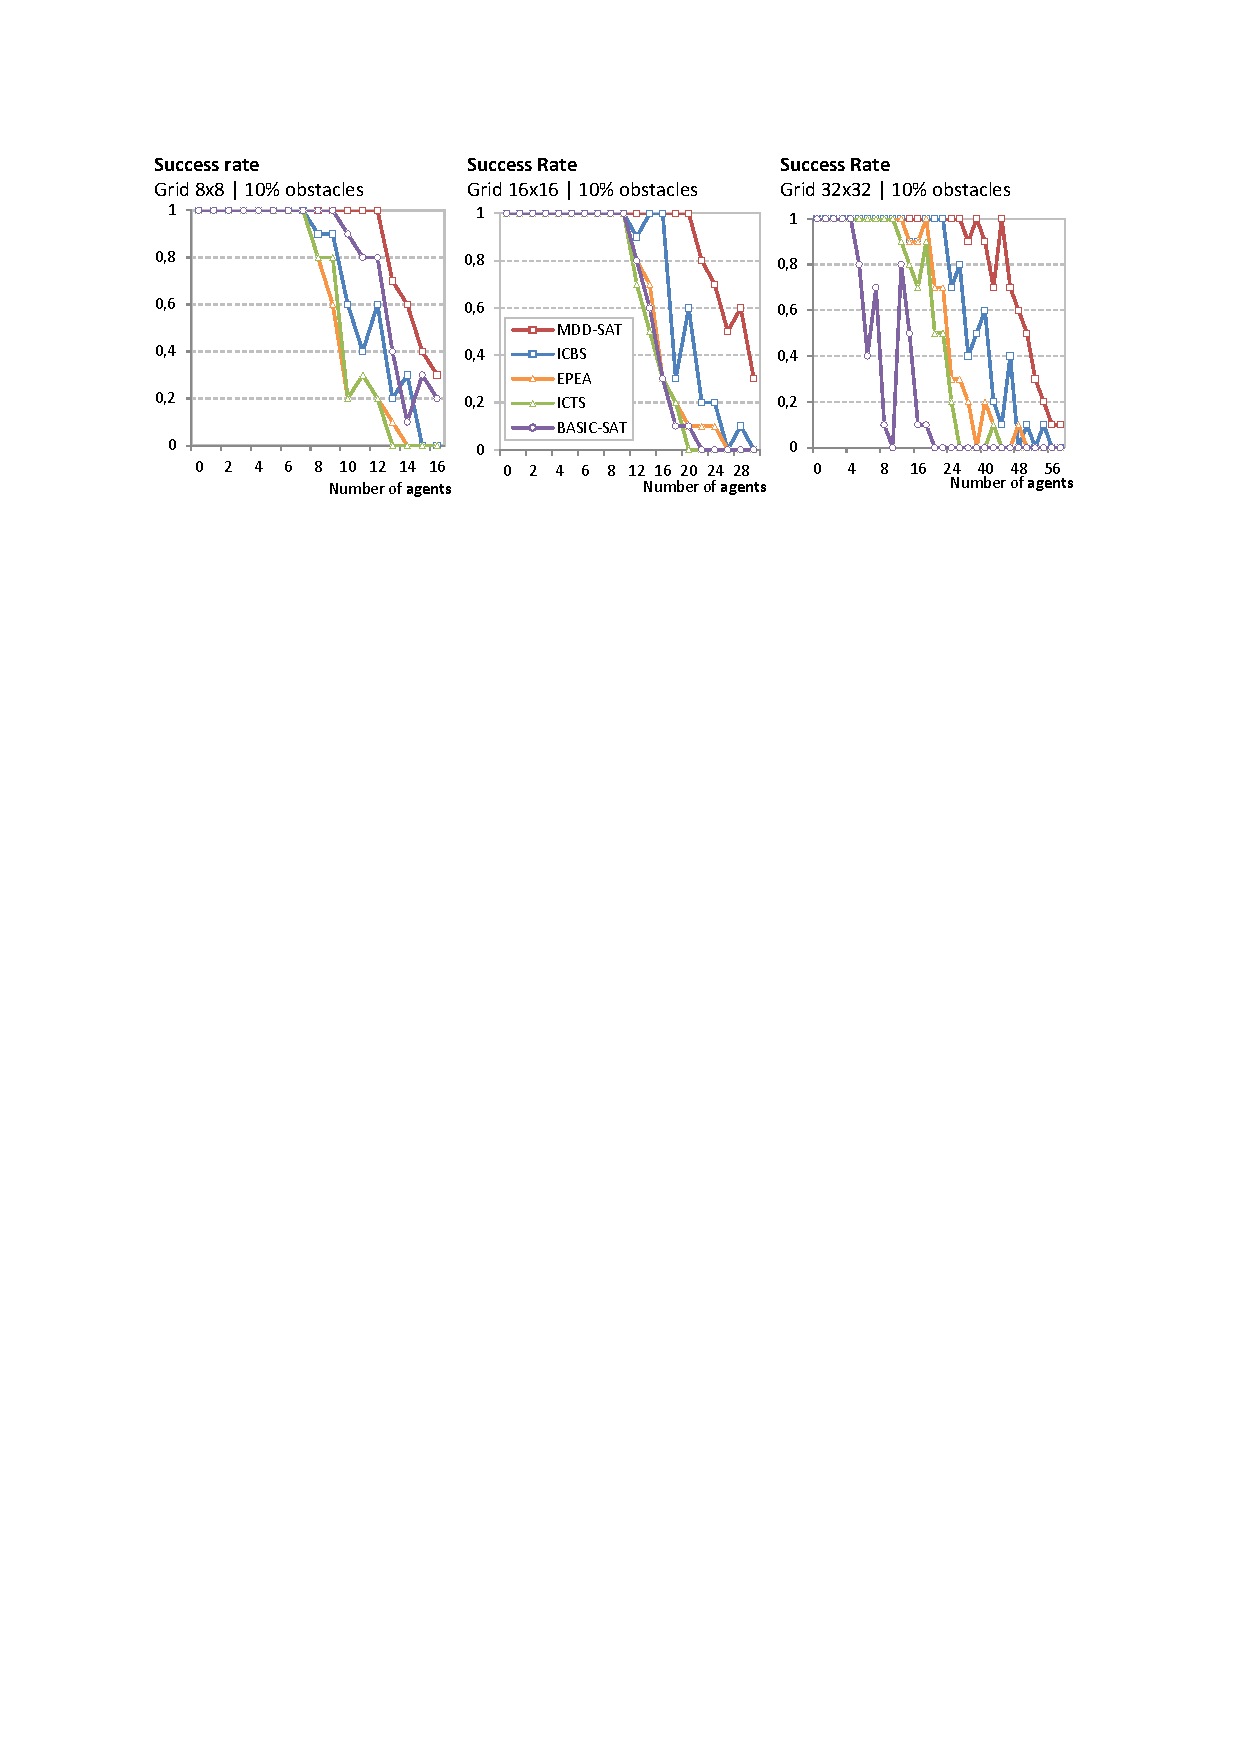
\includegraphics[trim={2.5cm 21.0cm 2.5cm 2.6cm},clip,width=\textwidth]{expr_grids-succ-rate.pdf}
\vspace{-0.4cm}
\caption{Success rate results for $8{}\times{}8$, $16{}\times{}16$, and $32{}\times{}32$ grids (10 instances per number of agents).}
\label{expr_grids-succ-rate}
\end{figure}

Figure~\ref{expr_grids-succ-rate} presents {\em success rate} results where each algorithm was given a time limit of 300 seconds (as was done by Sharon et al., 2013, Boyarski et al., 2015; Sharon, Stern, Felner, \& Sturtevant, 2015a). Success rate corresponds to percentage out of given 10 random instances solved within the time limit as a function of the number of agents (higher curves are better).

%\cite{DBLP:journals/ai/SharonSGF13,DBLP:conf/ijcai/BoyarskiFSSTBS15,SharonSFS15}).

\begin{figure}[h]
\centering
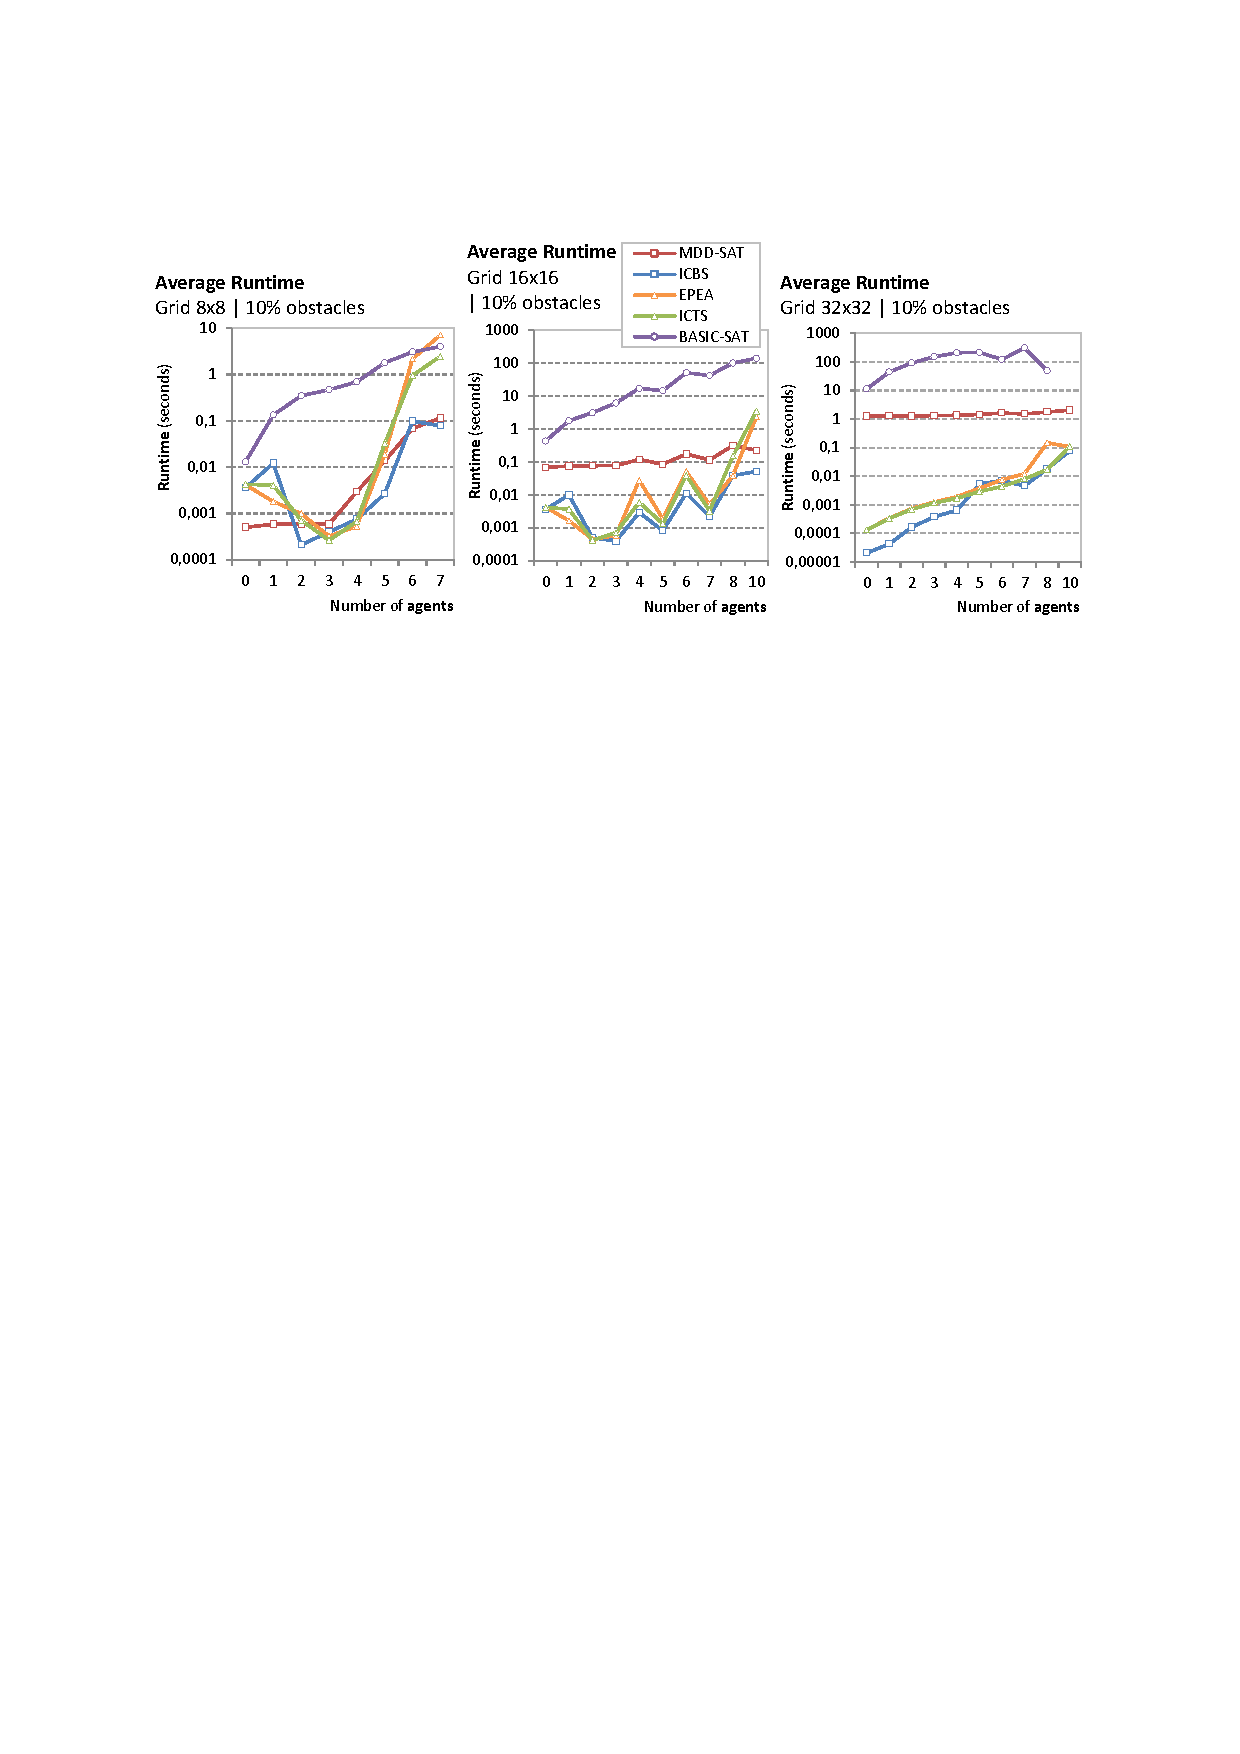
\includegraphics[trim={2.5cm 19.0cm 2.5cm 3.5cm},clip,width=\textwidth]{expr_grids-average.pdf}
\vspace{-0.4cm}
\caption{Average runtime for $8{}\times{}8$, $16{}\times{}16$, and $32{}\times{}32$ grids measured out of 10 instances per number of agents (vertical axis uses a logarithmic scale).}
\label{expr_grids-average}
\end{figure}

Figure \ref{expr_grids-average} reports the average runtime for instances that were solved
by all algorithms (lower curves are better). Here, we required $100\%$ success
rate for all the tested algorithms to be able to calculate the average runtime;
this is also the reason why the number of agents is smaller.

\begin{figure}[t]
\centering
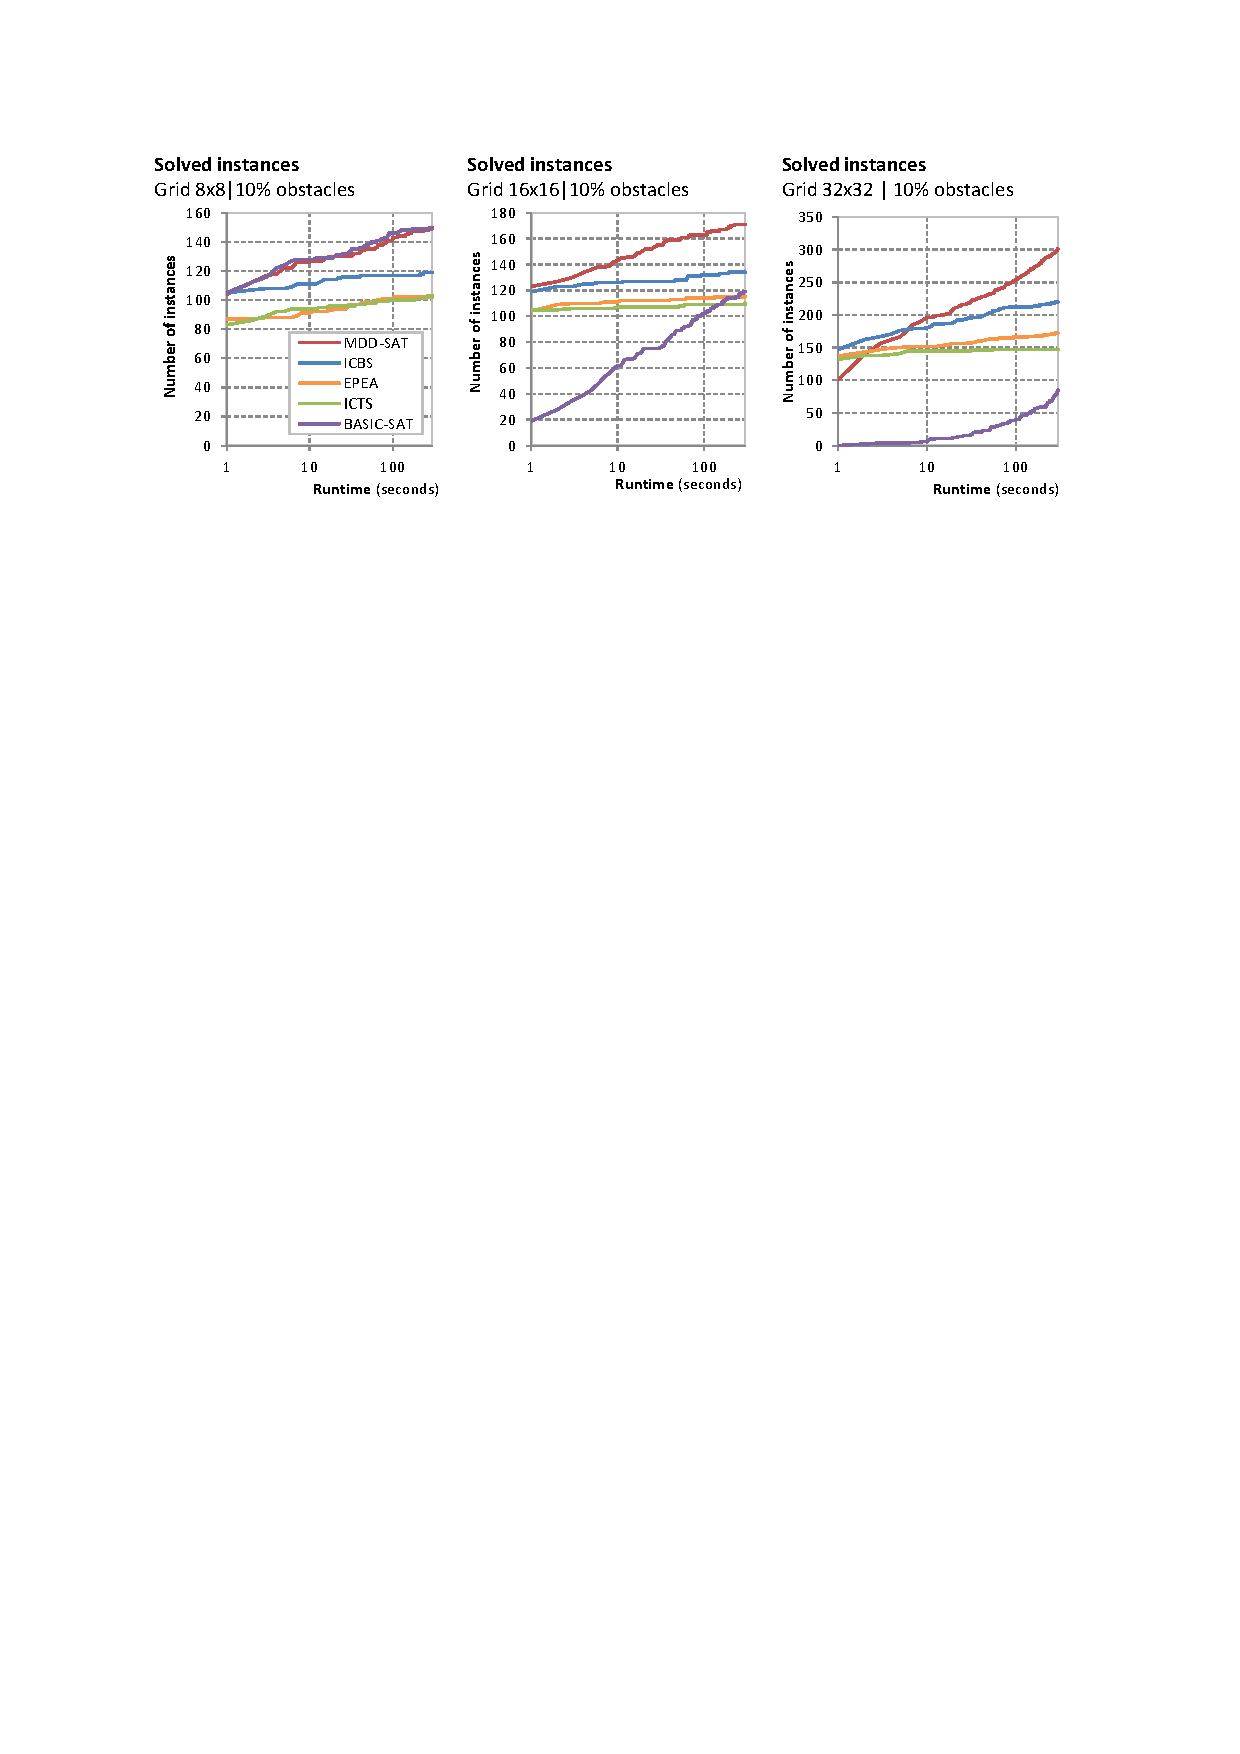
\includegraphics[trim={2.5cm 21.0cm 2.5cm 2.6cm},clip,width=\textwidth]{expr_grids-num-solved.pdf}
\vspace{-0.4cm}
\caption{Number of solvable instances in $8{}\times{}8$, $16{}\times{}16$, and $32{}\times{}32$ grids as a function of time limit (the horizontal runtime axis uses logarithmic scale).}
\label{expr_grids-num-solved}
\end{figure}

Figure \ref{expr_grids-num-solved} visualizes the results on $8{}\times{}8$, $16{}\times{}16$, $32{}\times{}32$ grid
in a different way. Here, we present the number of instances (out of all instances for all number of agents) that each method solved ($y$-axis) as a function of the elapsed time ($x$-axis). Thus, for example says that MDD-SAT was able to solve 145 instances in time less
than 10 seconds on the $16{}\times{}16$ (higher curves are better). A different view is provided when instances are sorted according to their runtimes for each individual tested algorithm (Figure~\ref{expr_grids-sorted}). The lower curve now represents a better performing algorithm.	

The first trend is that MDD-SAT significantly outperforms BASIC-SAT in all aspects. This shows the importance of developing enhanced SAT encodings for the MAPF problem. The performance of the BASIC-SAT encoding compared to the search-based algorithm degrades as the size of the grids grows larger: in the 8x8 grids it is second only to MDD-SAT, in the 16x16 grid it is comparable to most search-based algorithms, and in the 32x32 grid it is even substantially worse.

\begin{figure}[h]
\centering
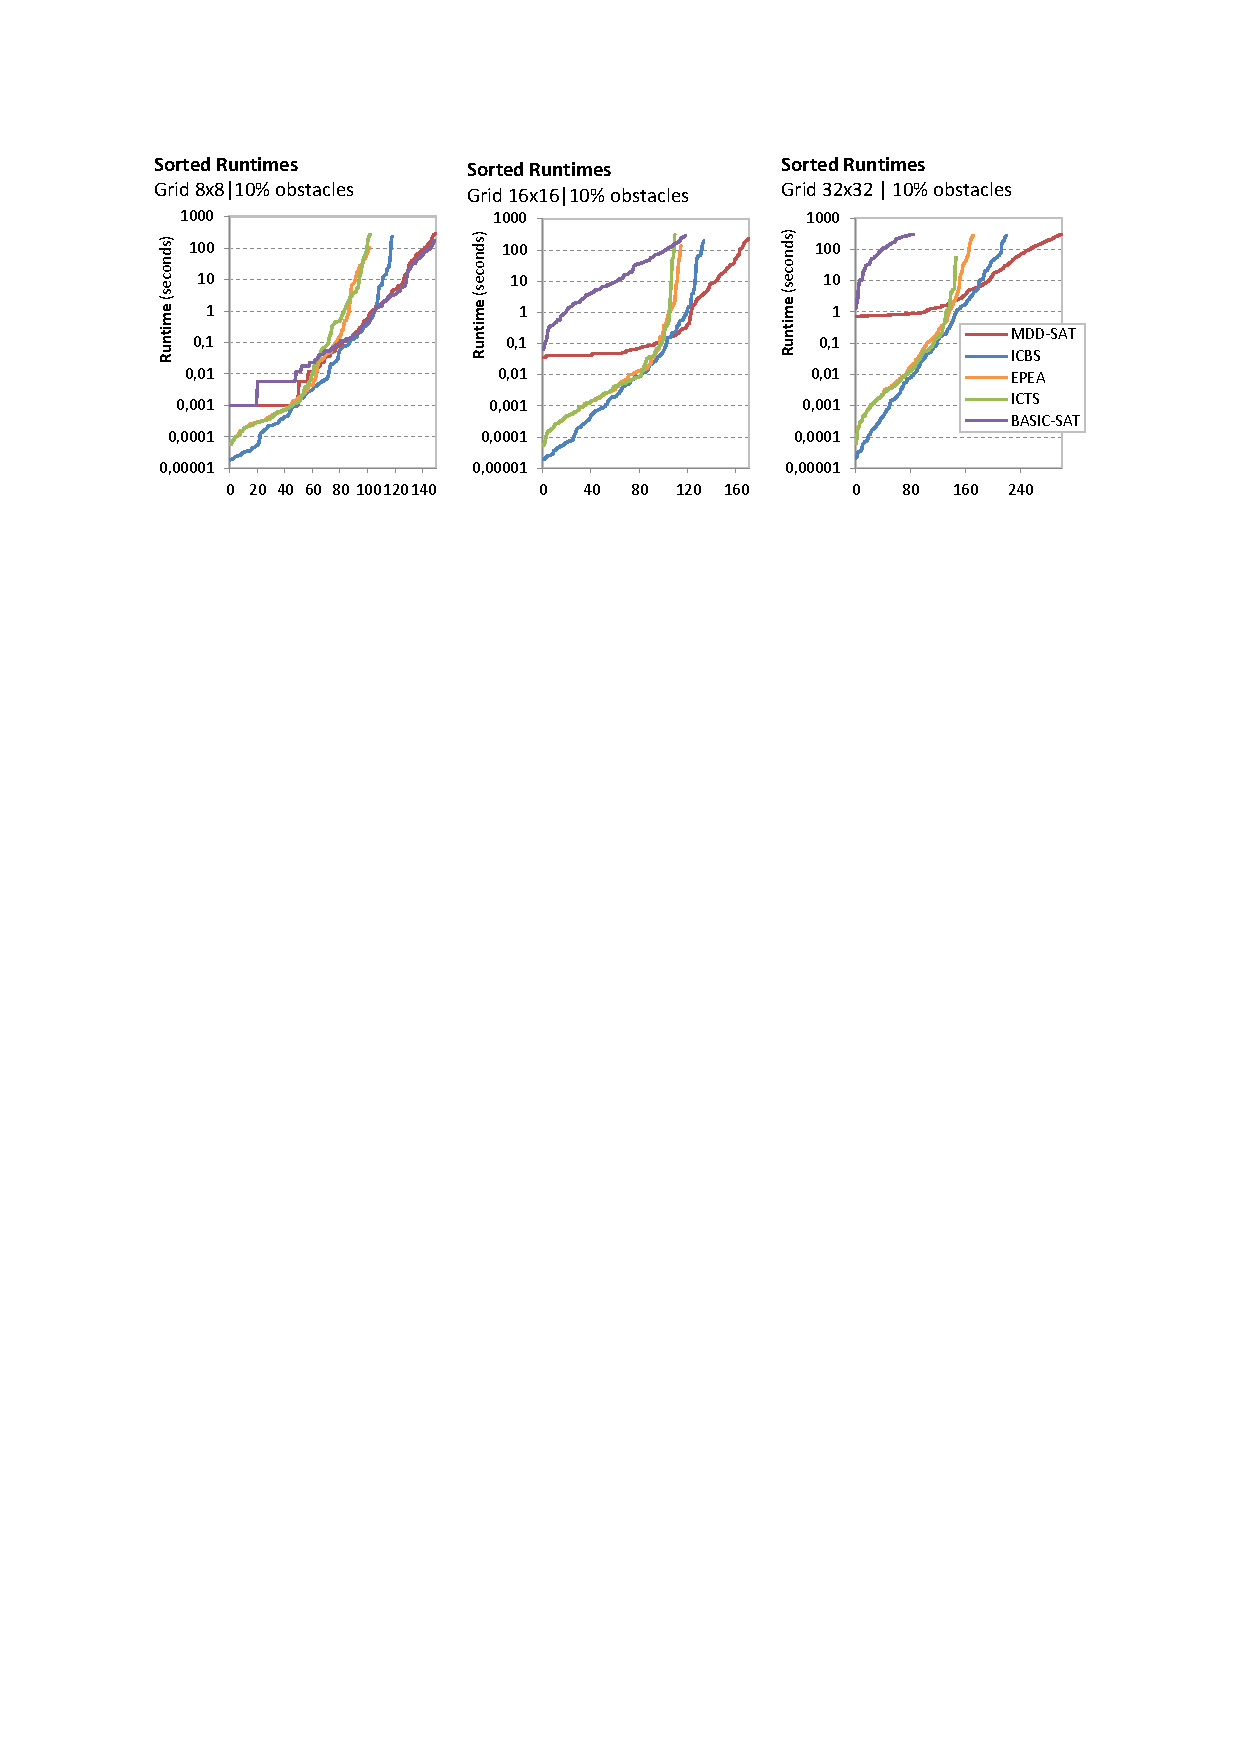
\includegraphics[trim={2.5cm 21.0cm 2.5cm 2.5cm},clip,width=\textwidth]{expr_grids-sorted.pdf}
\vspace{-0.4cm}
\caption{Sorted runtimes for $8{}\times{}8$, $16{}\times{}16$, and $32{}\times{}32$ grids (the horizontal axis corresponds to instances sorted differently for each tested algorithm).}
\label{expr_grids-sorted}
\end{figure}

In addition, a prominent trend observed in all the plots is that MDD-SAT has higher success rate and solves more instances than all other algorithms. In particular, in highly constrained instances (containing many agents) the MDD-SAT solver is the best option.

\begin{figure}[h]
\centering
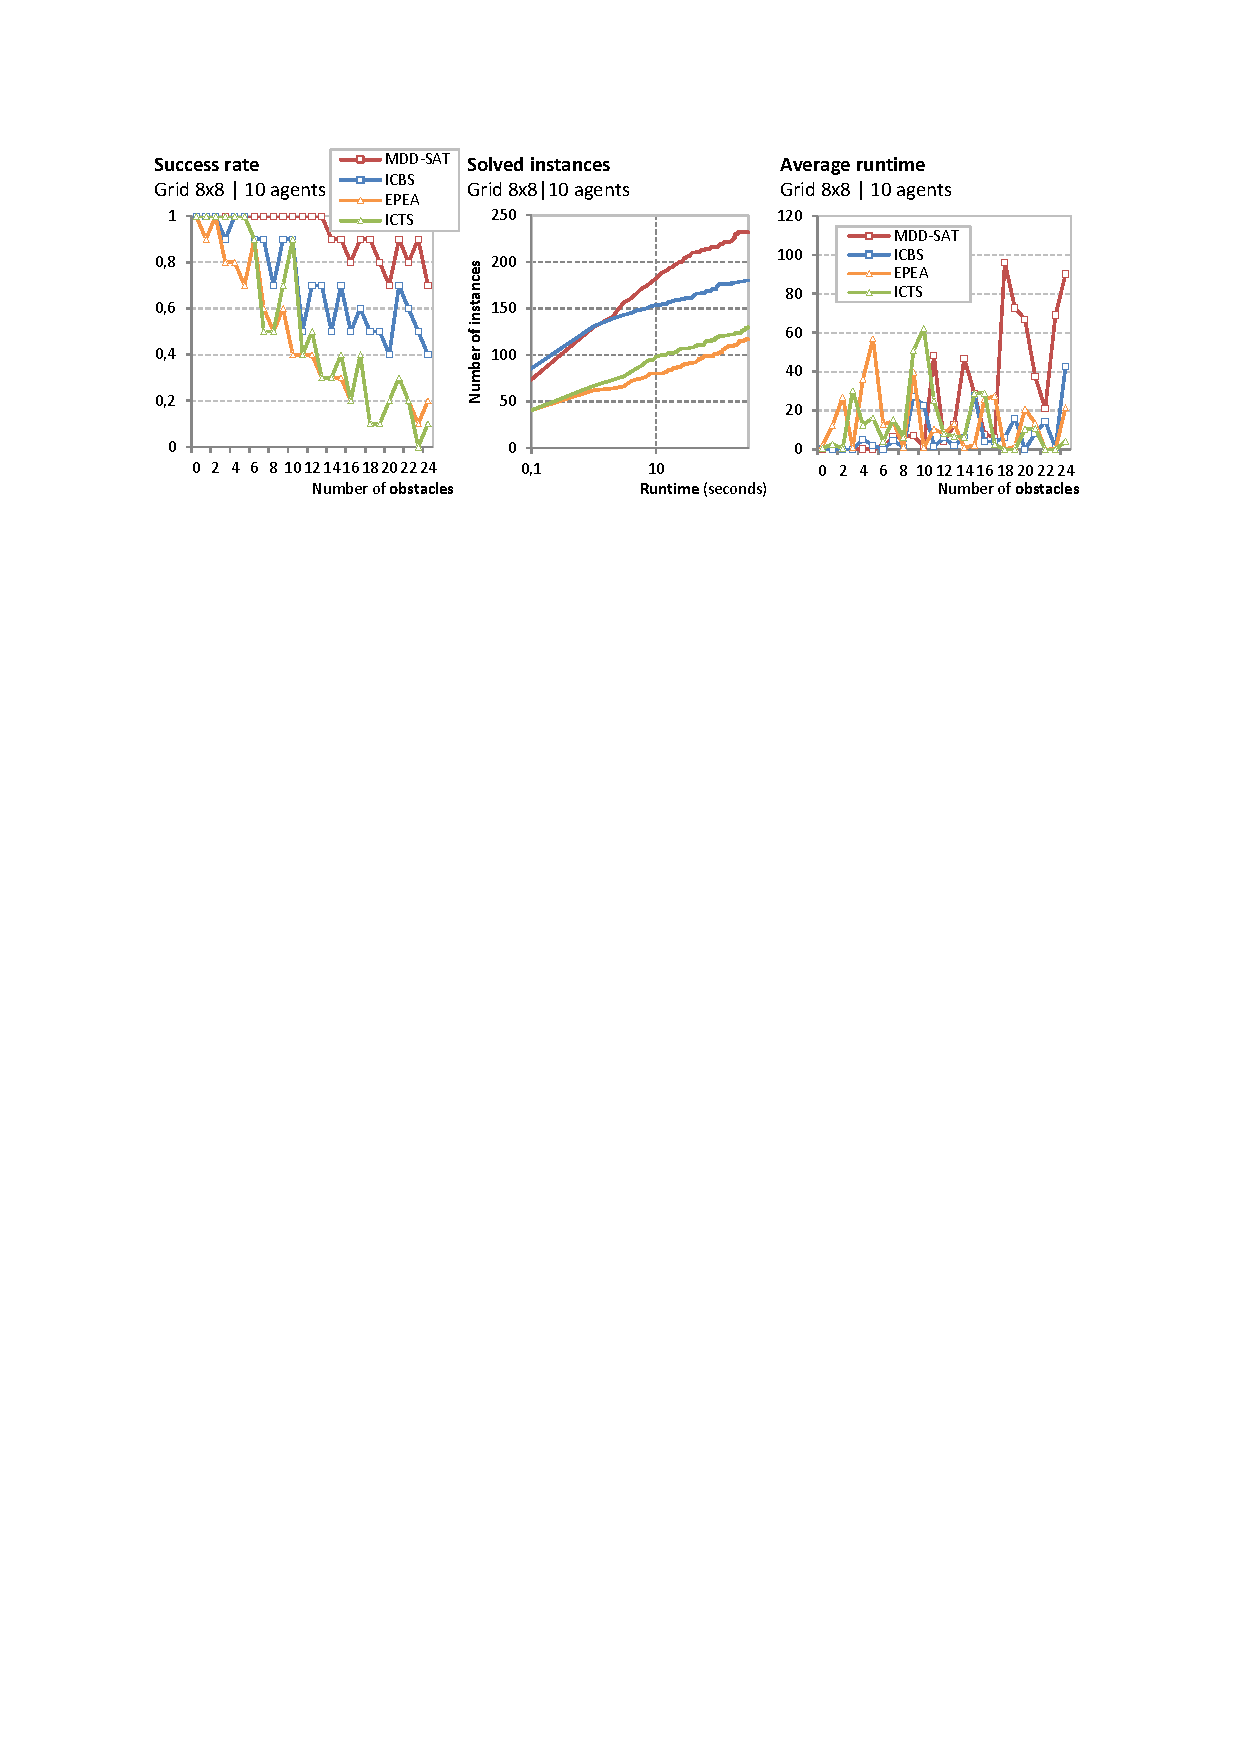
\includegraphics[trim={2.5cm 21.0cm 2.5cm 2.5cm},clip,width=\textwidth]{expr_obst-variation-8x8.pdf}
\vspace{-0.4cm}\caption{Success rate and runtime on the $8 \times 8$ grid with increasing
number of obstacles (out of 64 cells).} \label{figure-obstacles}
\end{figure}

However, on the $32{}\times{}32$ grid (rightmost figure) for easy instances when the available runtime was less than 10 seconds, MDD-SAT is weaker than the search-based algorithms. This is mostly due to the architecture of the MDD-SAT solver, which has an overhead of constructing the formula, running the external SAT solver, passing the input to it, and extracting the output from it (the truth-value assignment of variables needs to be interpreted back to agents' moves).

This effect is also seen in the 8x8 plot for the BASIC-SAT solver, which out of all solvers has the highest runtime for instances containing few agents. The effect of the overhead with calling the external SAT solver is multiplied by relatively inefficient formula based on TEGs in terms of its size.

Next, we varied the number of obstacles for the $8{}\times{}8$ grid with 10 agents to see the impact of shrinking free space and increasing the frequency of interactions among agents. Success rate, the number of solved instances, and the average runtime are shown in Figure~\ref{figure-obstacles}. BASIC-SAT is omitted in this experiment due to its weaker performance from the previous test. MDD-SAT has the highest success rate except for some easy instances (that needed up to 1 second) where ICBS was slightly faster, which is again due to the overhead in the setup of SAT solving by an external solver.

We observe counter-intuitive behavior of MDD-SAT here. Increasing the number of obstacles reduces the number of open cells. This is an advantage for the SAT formula generator in MDD-SAT as the formula has fewer variables and constraints. By contrast, the combinatorial difficulty of instances increases with adding obstacles for all the solvers as it means that graphs gets denser with agents (i.e., the ratio of agents to possible agent positions gets higher) and harder to solve.

The rightmost part of Figure~\ref{figure-obstacles} shows average runtime for each number of agents out of 10 instances being solved under the time limit. Here we can see that MDD-SAT tends to use more time in more difficult instances while other search based solvers tend to finish quickly on easier instances while being not successful on harder ones.

\pagebreak
\subsection{MDD-SAT and the Makespan Objective}

\begin{wrapfigure}{r}{0.5\textwidth}
\vspace{-1.0cm}
\begin{center}
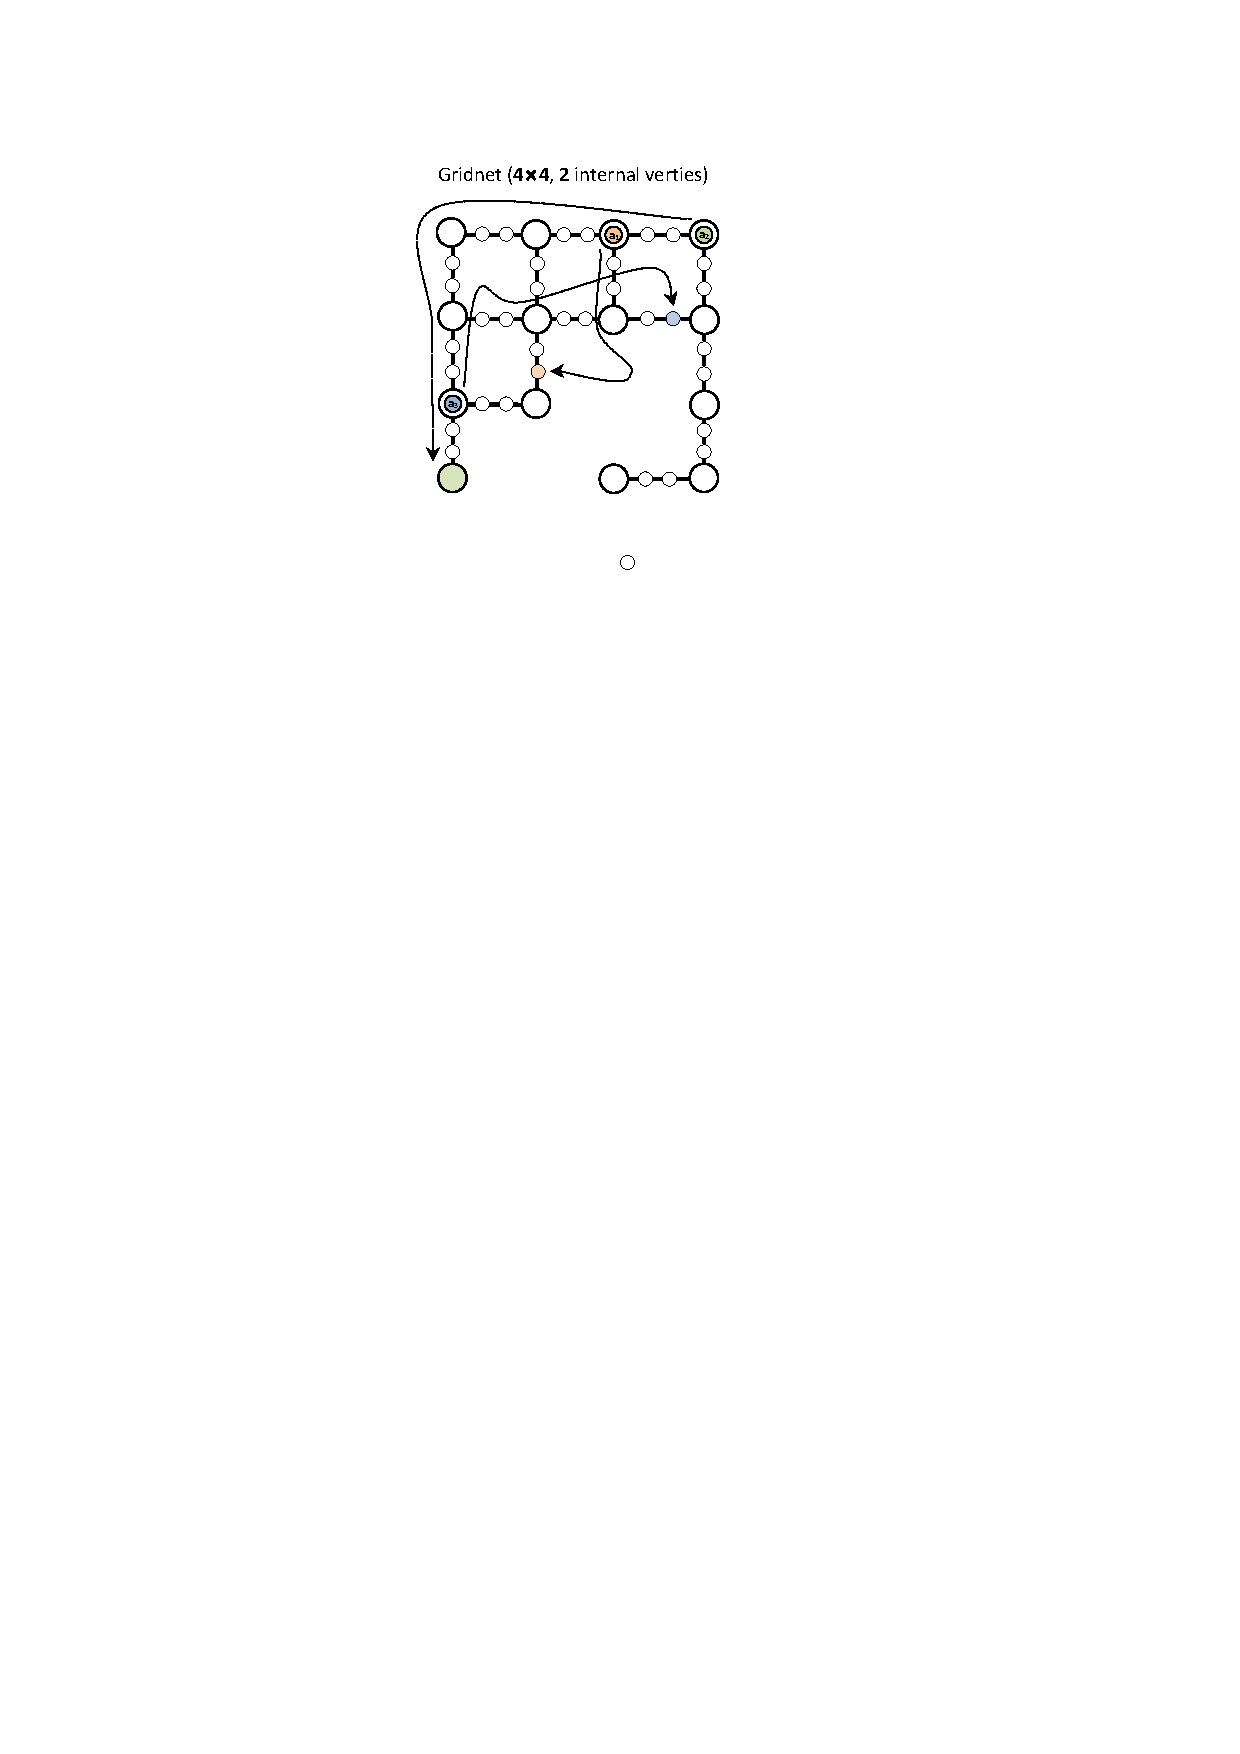
\includegraphics[trim={7.0cm 21.3cm 8.8cm 2.8cm},clip,width=0.35\textwidth]{fig_GRIDNET.pdf}
\end{center}
\caption{An example of MAPF with 3 agents on a $gridnet(4 \times 4, 2)$ graph originating from a $4 \times 4$ grid with obstacles.} \label{figure-GRIDNET}
\end{wrapfigure}


To provide more comprehensive picture we compare MDD-SAT with previous SAT-based solvers. However previous SAT-based solvers for MAPF using the \textsc{Matching} encoding (the solver called MATCHING-SAT) \cite{DBLP:conf/ictai/Surynek14} and the \textsc{Direct} encoding (DIRECT-SAT) \cite{DBLP:conf/micai/Surynek14} are implemented for the makespan objective. Hence comparing MDD-SAT directly with these solvers is not relevant. Therefore we modified MDD-SAT for the makespan objective as first suggested by Surynek et al.  \citeyear{DBLP:conf/socs/SurynekFSB16}. The modified solver will be denoted MDD-SAT(make). 

The modification of MDD-SAT for the makespan objective consists in removing the cost bound $\xi$ from the formula. That is, cardinality constraints concerning bounding $\xi$ are omitted. The rest of iterative scheme that increases makespan $\mu$ is kept. In the course of execution of MDD-SAT(make), we again generate the sequence of MDDs. However these MDDs are different from those in MDD-SAT for the sum-of-costs where each MDDs is constructed for different cost $\xi_0(a_i) + \Delta$. We need to ensure that each agent can use all cost bounded only by common makespan $\mu$ applicable to all agents. Hence all MDDs in MDD-SAT(make) are constructed for cost $\mu=\mu_0 + \Delta$, where $\mu_0=max_{i=1}^k\{\xi_0(a_i)\}$.

Agents for which $\xi_0(a_i) < \mu_0$ are given more freedom due to larger MDDs in MDD-SAT(make) compared to the original MDD-SAT. Due to this relaxation and absence of the overall cost bound represented by the cardinality constraint the resulting encodings in MDD-SAT(make) is simpler and less constrained. Therefore we hypothesize that MDD-SAT(make) will be faster than MDD-SAT.

We also modified search-based solvers \textsc{Icts}, \textsc{Epea}*, and \textsc{Icbs} for the makespan objective. Since these MAPF solving algorithms are defined for any cumulative cost, their adaptation for the makespan objective is done in straightforward way by replacing the calculation of sum-of-costs by the calculation of makespan. The modified algorithms are denoted \textsc{Icts}(make), \textsc{Epea}*(make), and \textsc{Icbs}(make).

Comparison of sum-of-costs and makespan variants of all above-mentioned algorithms on 4-connected grid $16{}\times{}16$ is shown in Figure \ref{figure-makespan-net-cube} (upper part). The figure shows sorted runtimes for all instances solved under given timeout of 300 seconds (lower line is better). We put results for both objectives into the same plot to see both: comparison of different algorithms for single objective and comparison of single algorithm across different objectives.

Given the results, it cannot be universally said that the makespan objective is easier than sum-of-costs. \textsc{Epea}* performs better than \textsc{Epea}*(make) while in the case of \textsc{Icts} and \textsc{Icbs}, the makespan objective is easier. Search-based solvers perform better than compilation-based solvers in easier instances but as the difficulty grows their runtime goes up faster than in compilation-based solvers. The notable exception is MDD-SAT, which is competitive to search-based solvers even for easy instances.

\begin{wrapfigure}{l}{0.5\textwidth}
\begin{center}
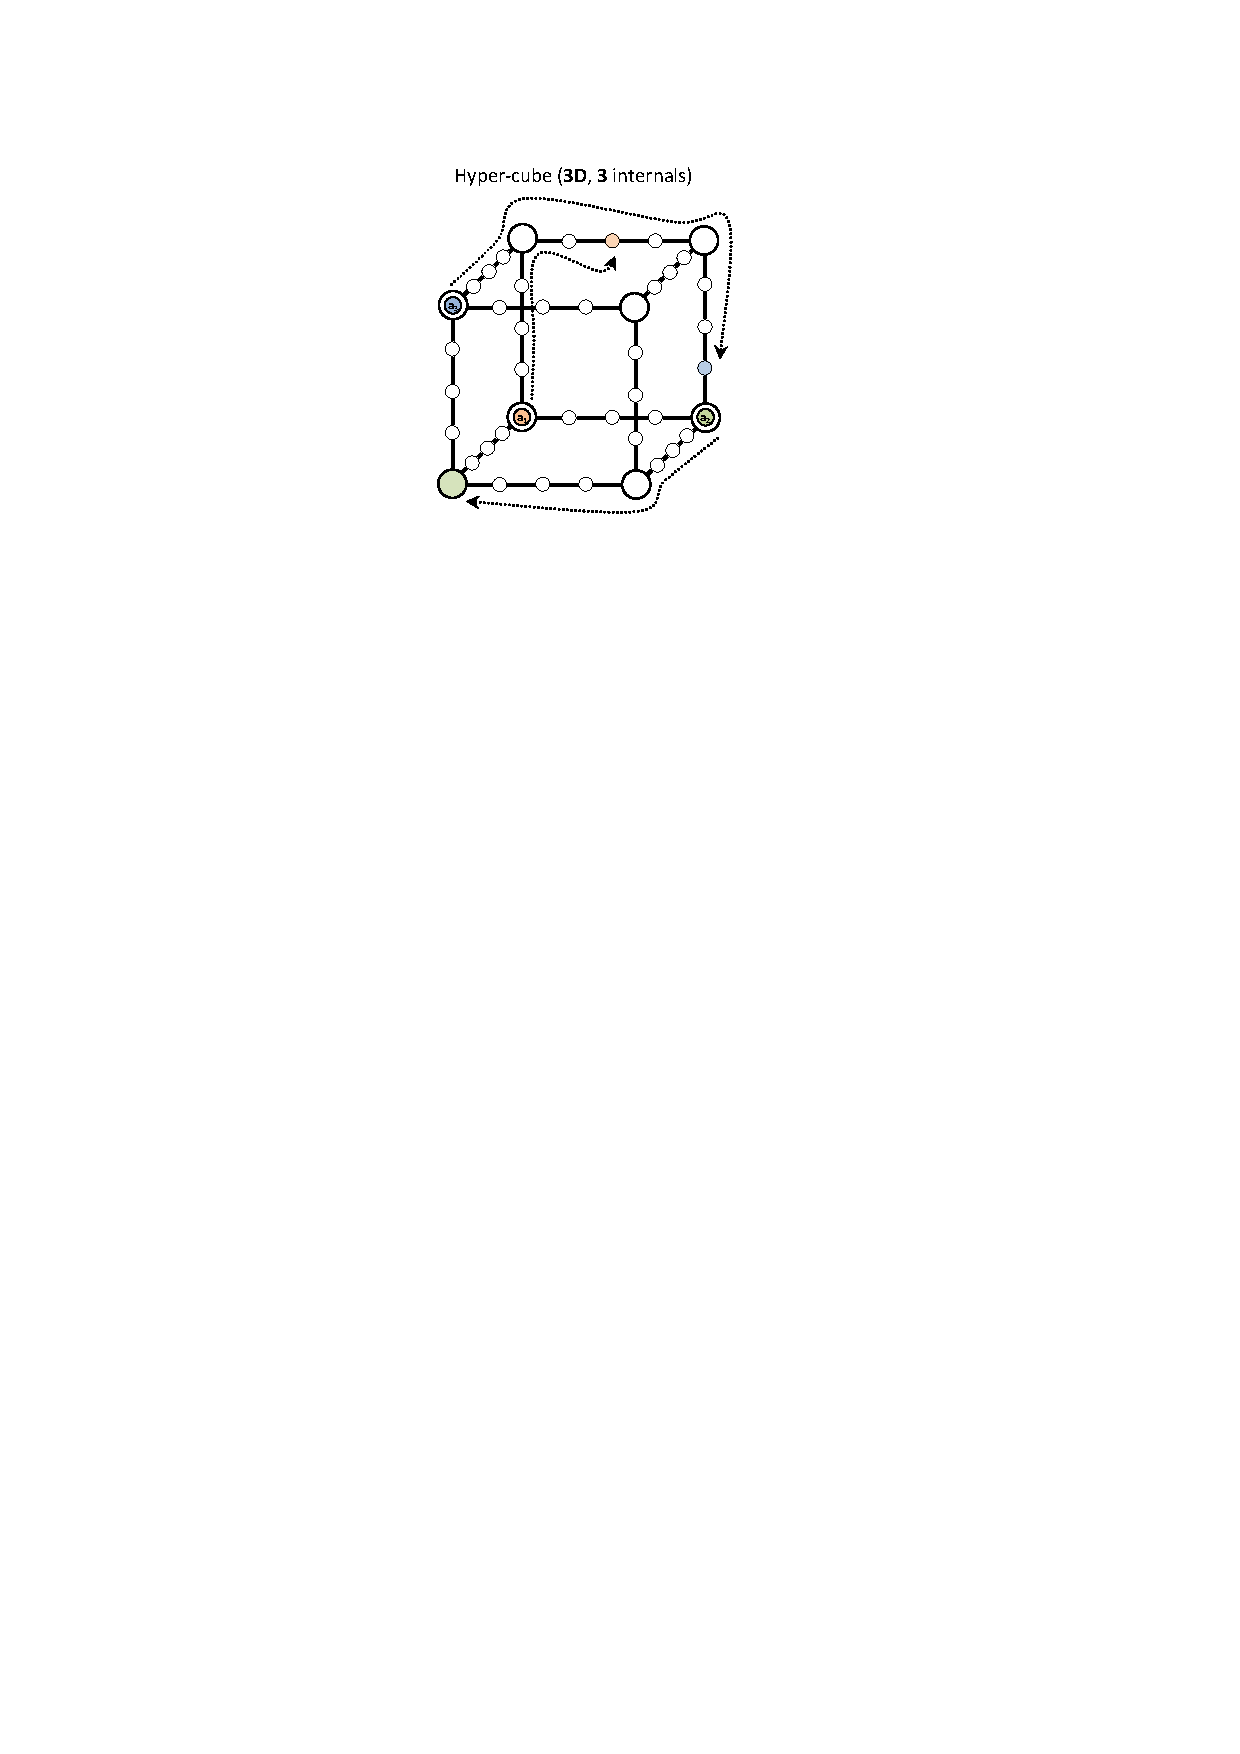
\includegraphics[trim={7.3cm 21.0cm 8.6cm 2.8cm},clip,width=0.35\textwidth]{fig_HYPER.pdf}
\end{center}
\caption{An example of MAPF with 3 agents on a $hypercube(3D, 3)$.} \label{figure-HYPER}
\end{wrapfigure}

Comparison across SAT-based solvers shows that the previous MATCHING-SAT solver is far behind DIRECT-SAT and MDD-SAT(make) while the latter two solvers are very close to each other, still MDD-SAT(make) is faster. MATCHING-SAT uses the {\em log-space} encoding \cite{DBLP:books/sp/Petke15} for representation of the decision variables, which seemingly does not perform well due to poor {\em Boolean constraint propagation} (BCP) /{\em unit propagation} (UP) \cite{DBLP:journals/jlp/DowlingG84} on top of this encoding. Both DIRECT-SAT and MDD-SAT(make) are based on the {\em direct encoding} \cite{DBLP:journals/constraints/TamuraTKB09}, which, on the other hand, supports BCP/UP well.

Several trends can be observed in the results. The hypothesis that MDD-SAT(make) performs better than MDD-SAT is confirmed by the results. However MDD-SAT(make) starts to prevail only in difficult problems where runtime of MDD-SAT grows much faster towards the time limit. The explanation of this behavior is that in larger and more difficult instances the cost bound represented by the cardinality constraint has more significant aggravating effect with respect to the performance.

In addition to square grids, we tested SAT-based solvers on other types of graphs representing different structure and connectivity to see whether it has any impact on
the difficulty of finding optimal solution by a particular solver. We used two types of graphs:

\begin{itemize}
\item a {\bf gridnet} graph, which can be constructed by starting with a 4-connected grid with obstacles (discussed previously) where edges are replaced by paths consisting of non-zero number internal vertices. Gridnet graphs originating from a 4-connected grid of size $m \times m$ where edges are replaced by paths with $p$ internal vertices are denoted $\mathit{gridnet}(m \times m, p)$. Example of gridnet graph denoted $\mathit{gridnet}(4 \times 4, 2)$ is shown in Figure \ref{figure-GRIDNET} - it is constructed from 4-connected grid $4 \times 4$ taken from Figure \ref{figure-MAPF} where edges are replaced by paths containing 2 internal vertices.

\item a {\bf hyper-cube} graph, which is constructed by starting with a {\em hyper-cube} of certain dimension. Similarly to previous construction, we take the standard $d$-dimensional hyper-cube graph as a basis. Then each edge in the starting hype-cube is replaced by a path consisting of non-zero number of internal vertices. Analogously to the previous notation $\mathit{hypercube}(dD, p)$ denotes the hyper-cube graph originating from a $d$-dimmensional hyper-cube where edges are replaced by paths consisting of $p$ internal vertices. An example of 3-dimensional hyper-cube (that is a cube) with 3 internal vertices per edge - denoted as $\mathit{hypercube}(3D, 3)$ - is shown in Figure \ref{figure-HYPER}.
\end{itemize}

\begin{figure}[h]
\centering
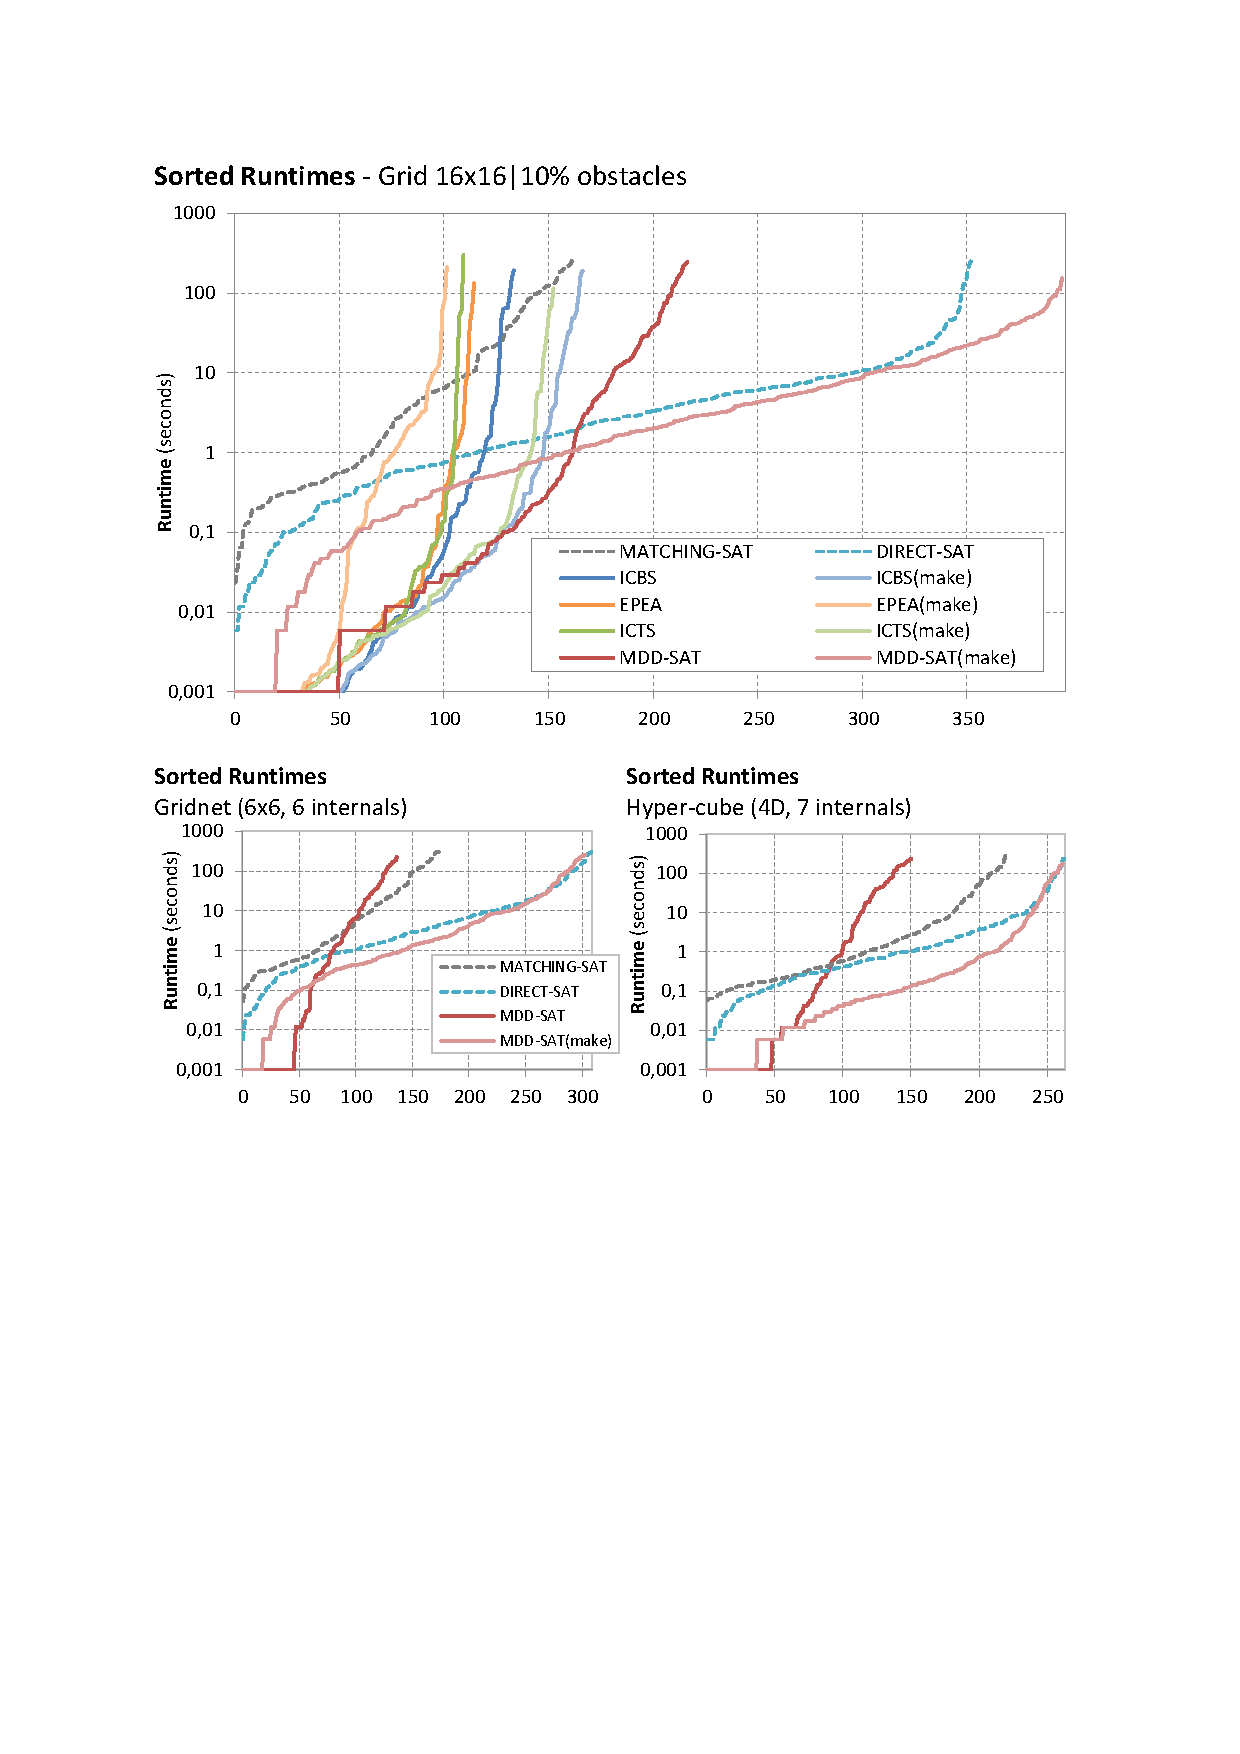
\includegraphics[trim={2.5cm 10.5cm 2.5cm 2.8cm},clip,width=0.9\textwidth]{expr_make+net-cube.pdf}
\vspace{-0.4cm}
\caption{MDD-SAT with the makespan objective and the sum-of-costs objective compared to \textsc{Icts} and \textsc{Icbs} and previous makespan-optimal SAT-based solvers MATCHING-SAT and DIRECT-SAT (lower line means better solver).} \label{figure-makespan-net-cube}
\end{figure}

Paths replacing edges of the \emph{high level} graph structure represent narrow corridors where it is expected that avoidance of agents will be more difficult than in the standard 4-connected grids. Moreover there is also practical motivation for such graphs. Floor-plans of many warehouses or shop-like spaces show similar structure where storage areas are surrounded by narrow aisles \cite{DBLP:conf/atal/ClaesOBT17,DBLP:conf/icarcv/TsangNWS18}.

In the experiment with {\em gridnet} and {\em hyper-cube} graphs we need to omit comparison with \textsc{Icts} and \textsc{Icbs} since their implementation does not support graphs other than grids. We also omit BASIC-SAT in this experiment. Results for $\mathit{gridnet}(6 \times 6, 6)$ and  $\mathit{hypercube}(7D, 7)$ are shown in Figure \ref{figure-makespan-net-cube} (lower part). The figure shows sorted runtimes of each tested solver across all instances solvable under the time limit (lower line corresponds to a better solver).

The relative ordering of individual solvers in terms of their performance for the makespan objective is almost the same as for the $16{}\times{}16$ grid. The notable difference is only diminishing difference between MDD-SAT(make) and DIRECT-SAT on hard instances. We attribute this to relatively long makespans in case of hard instances. Moreover in {\em gridnet} and {\em hyper-cube} tend to lead to long makespans because of the presence of narrow corridors in these graphs. When the makespan is long the effect of using MDDs compared to the TEG-based time expansion of the underlying graph is negligible.

The relative performance of sum-of-costs MDD-SAT compared to makespan-optimal solvers is far worse than in the $16{}\times{}16$ grid. While in the grid case MDD-SAT clearly dominates in easy instance no such clear dominance is observed in {\em hyper-cube} and only less significant dominance in easy cases is observed in the {\em gridnet} graph. Moreover the worst-performing makespan-optimal solver, MATCHING-SAT, eventually outperforms MDD-SAT for harder instances, which never happened in the grid case. We explain this trend by a great difference between the true optimal sum-of-costs and the lower bound estimation $\xi_0$ calculated as the sum of lengths of shortest paths: $\sum_{i=1}^k{\xi_0(a_i)}$. This difference is greater in case of {\em gridnet} and {\em hyper-cube} than in 4-connected grids due to narrow corridors where avoidance between agents is necessary. In such a case the lower bound estimation is inaccurate because it ignores this avoidance. This altogether leads to more iterations of the MDD-SAT algorithm. Moreover the sub-formula encoding the cardinality constraint representing the cost bound tends to be more complex in such a case.

\subsection{Experiments with Large Maps}

Experiments with MDD-SAT on large grid-based maps is presented in this section. We used benchmarks from  Sturtevant's repository \cite{sturtevant2012benchmarks} - three structurally different Dragon Age Origin (DAO) maps denoted as \texttt{brc202d}, \texttt{den520d}, and \texttt{ost003d}, which are a standard benchmark for MAPF (see Figure \ref{figure-maps}), are used. The size of the underlying grids for these maps is: $530{}\times{}481$ in \texttt{brc202d},  $256{}\times{}257$ in \texttt{den520d}, and $194{}\times{}194$ in \texttt{ost003d}. The relative size of the map belonging to the free space is depicted in Figure \ref{figure-maps}.

\begin{figure}[h]
\centering
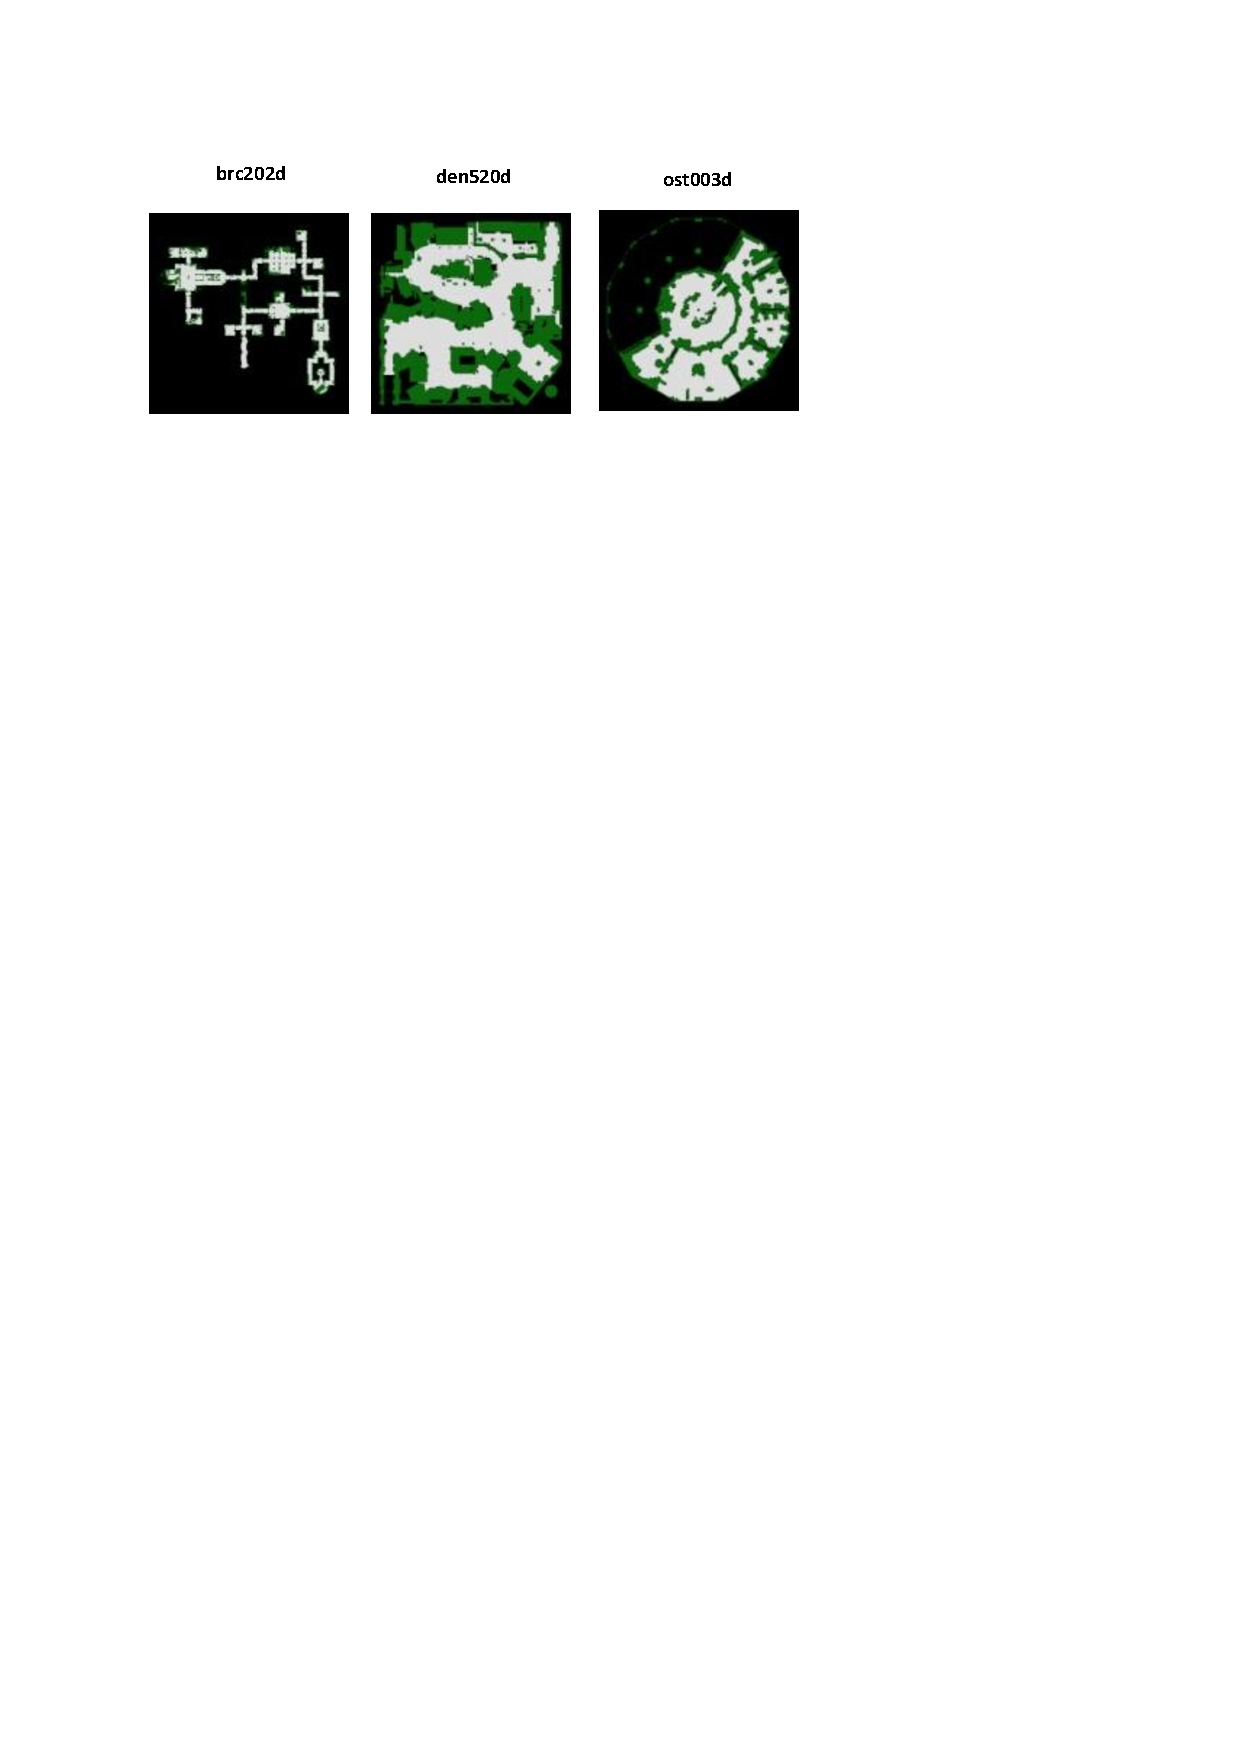
\includegraphics[trim={2.5cm 22.0cm 7cm 2.7cm},clip,width=0.75\textwidth]{fig_maps.pdf}
\vspace{-0.4cm}\caption{Dragon Age maps  include: narrow corridors in \texttt{brc202d}, large open space in \texttt{den520d}, and open space with almost isolated rooms in \texttt{ost003d}.} \label{figure-maps}
\end{figure}

The tests include optimal sum-of-costs algorithms  MDD-SAT, \textsc{Icts} and \textsc{Icbs} that were compared on instances containing 16, 24, and 32 agents in the selected DAO maps. To obtain instances of various difficulties we varied the average distance of agents from their goals. This particular measure is important for MDD-SAT as the distance of agent from its goal is the major parameter that determines the size of MDDs being generated during the solving process. The greater the distance is the larger MDD is produced and the instance is expected to be harder for MDD-SAT.

\begin{table}
\centering
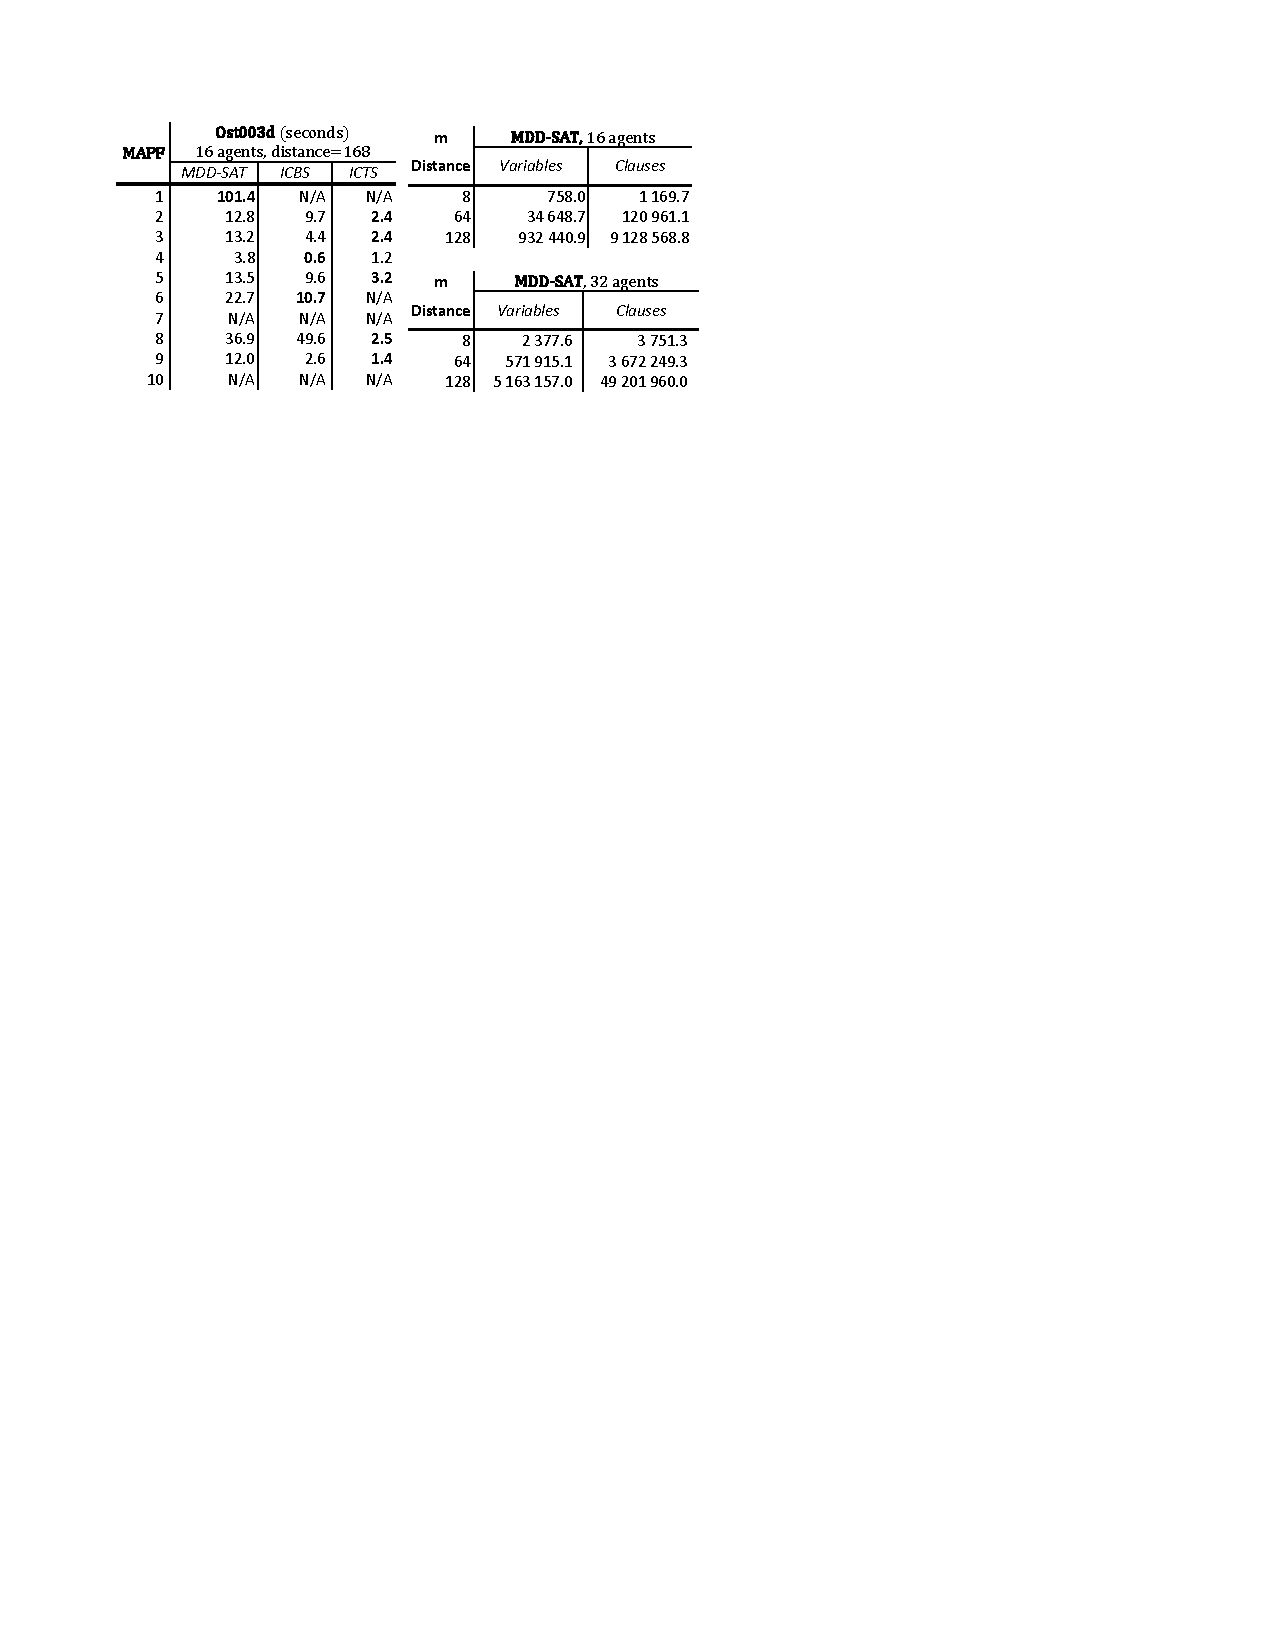
\includegraphics[trim={2cm 21.4cm 9.7cm 2.1cm},clip,width=0.75\textwidth]{table_ost003.pdf}
\caption{Runtime for 10 instances (left) and the average size
of the MDD-SAT formulae for \texttt{ost003d} (right)}\label{table_ost003}
\end{table}

\begin{figure}[h]
\centering
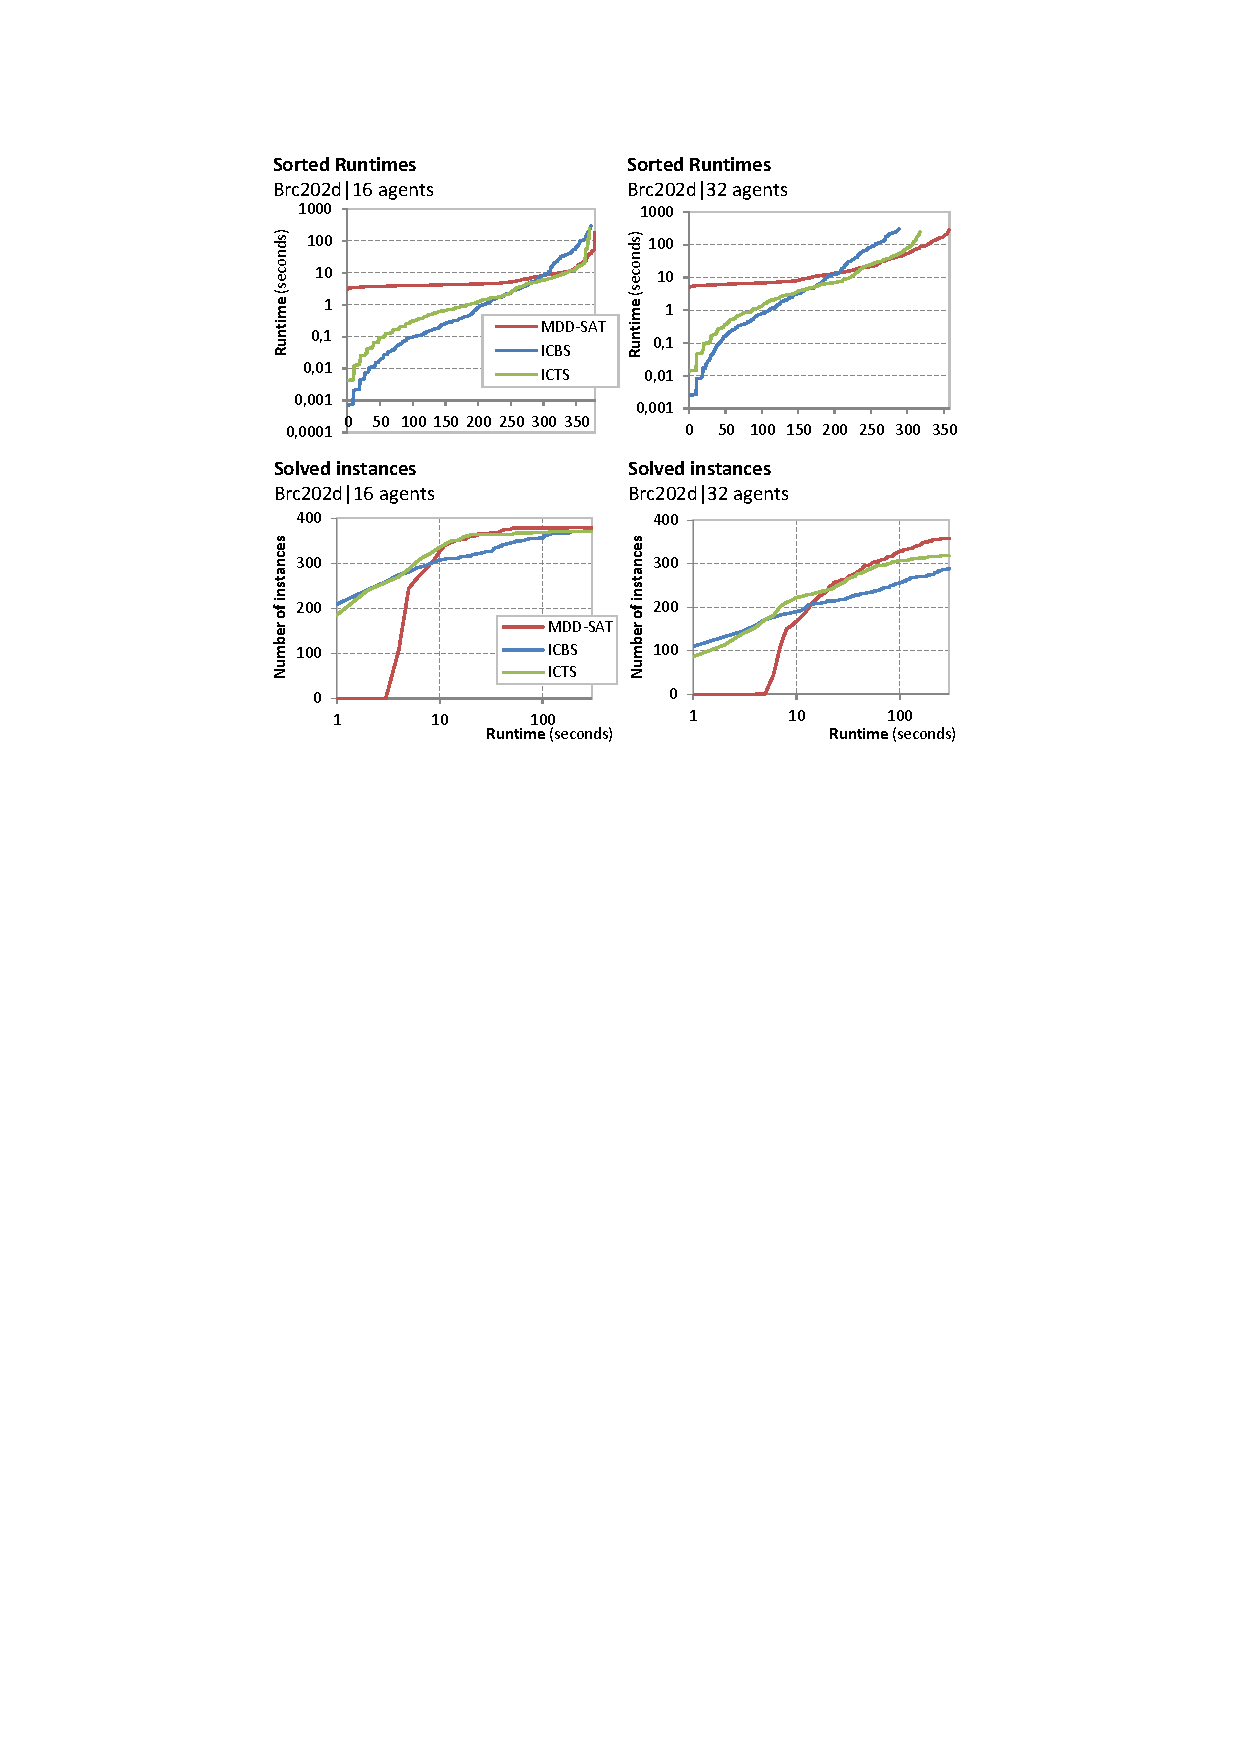
\includegraphics[trim={2.5cm 17.0cm 2.5cm 2.5cm},clip,width=1.0\textwidth]{expr_brc202_sorted.pdf}
\vspace{-0.6cm}\caption{Runtime results for \texttt{brc202d} DAO map. Sorted runtimes (top) and number of solved instances as a function of time are shown (bottom).}
\label{figure-brc202-sorted}
\end{figure}

\begin{figure}[h]
\centering
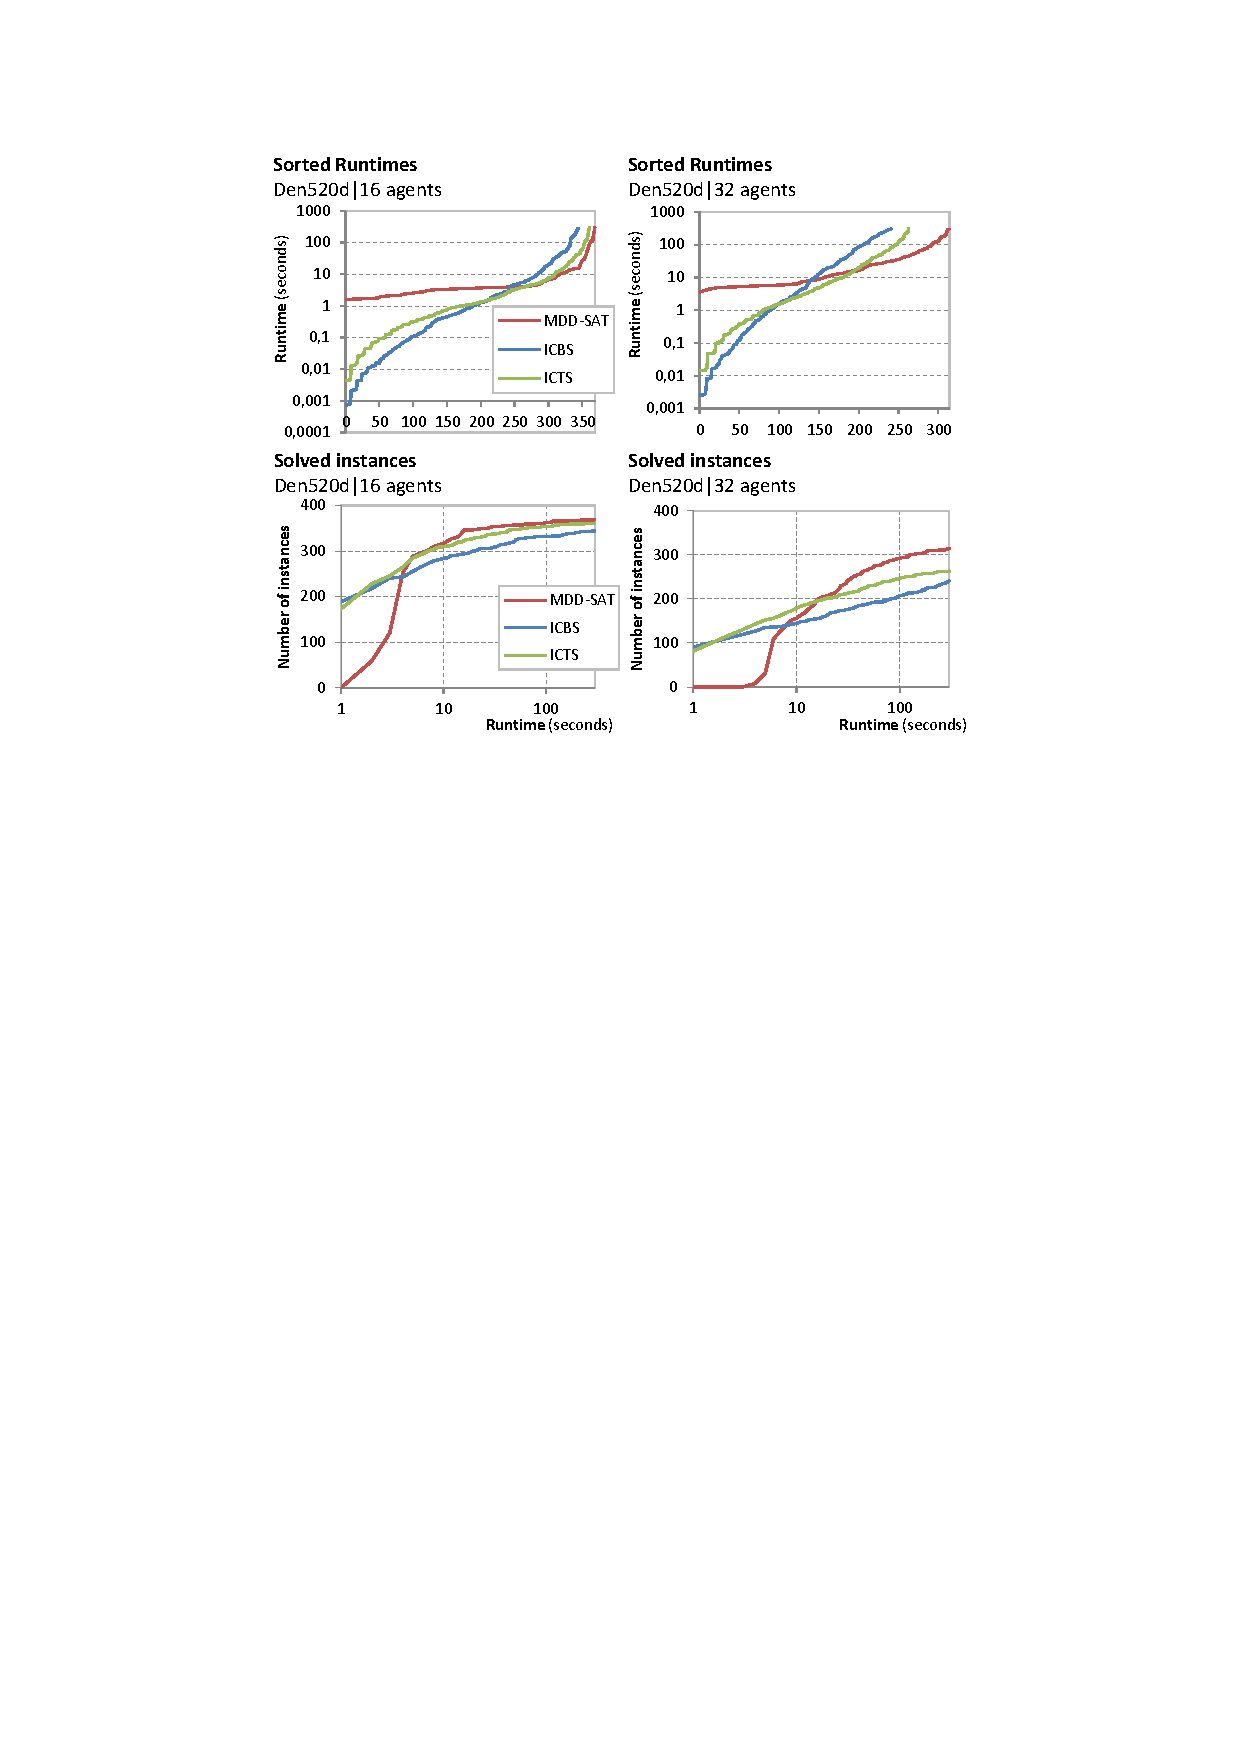
\includegraphics[trim={2.5cm 17.0cm 2.5cm 2.6cm},clip,width=1.0\textwidth]{expr_den520_sorted.pdf}
\vspace{-0.6cm}\caption{Runtime results for \texttt{den520d} DAO map. Sorted runtimes (top) and number of solved instances as a function of time are shown (bottom).}
\label{figure-den520-sorted}
\end{figure}

\begin{figure}[h]
\centering
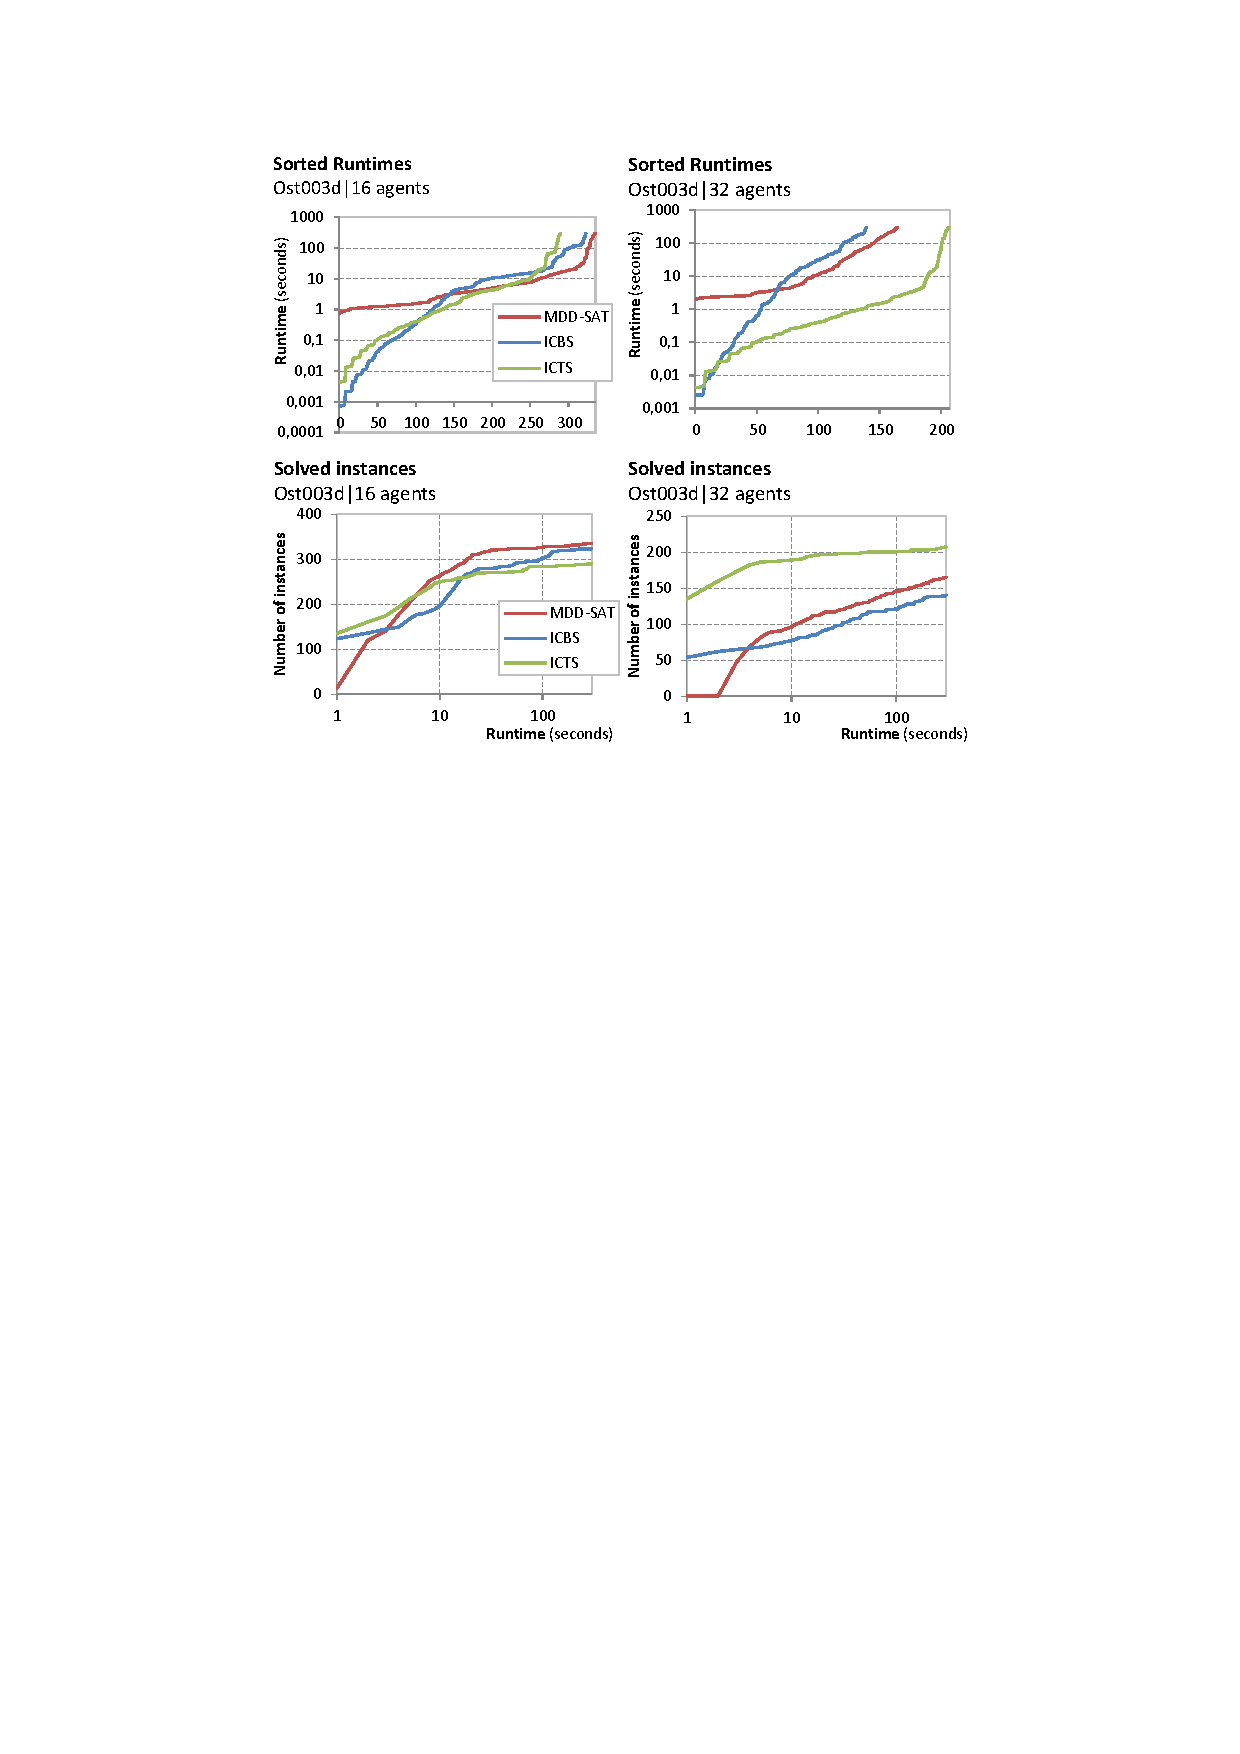
\includegraphics[trim={2.5cm 17.0cm 2.5cm 2.6cm},clip,width=1.0\textwidth]{expr_ost003_sorted.pdf}
\vspace{-0.6cm}\caption{Runtime results for \texttt{ost003d} DAO map. Sorted runtimes (top) and number of solved instances as a function of time are shown (bottom).}
\label{figure-ost003-sorted}
\end{figure}

The initial positions of agents is set randomly. Given the average distance, the goals for agents were generated in two steps: {\bf (i)} Potential goals for each agent were generated by long random walk in the graph in order to ensure solvability while for each potential goal its distance from the initial position was kept. {\bf (ii)} Then random goal from potential goals for each agent was selected using the uniform distribution across distances from the initial position so that the given average distance is obtained. The mean distance from initial positions is varied from 8 up to 320 using step 8. Ten random instance were generated per distance. The maximum mean distance was set so that no of the tested algorithms was able to solve instances for the maximum average distance given the time limit of 300 seconds.

The illustration of the average size of formulae generated by MDD-SAT on \texttt{ost003d} is shown in Table \ref{table_ost003} (right). For greater distance between the initial positions and the goals we can see rapid growth of the size of formulae. For the distance being increased twice from 64 to 128 the size of formulae in terms of the number of clauses increased 13-times for 32 agents, but 76 times for the 16 agents case. The size of formula is directly determined by the size of MDDs being generated whose size is proportional to the number of time expansions that is correlated with the agent's distance to the goal. The observed rapid growth of the size of formulae however needs additional explanation. We also need to take into account that using MDDs for great distances from the goal not only increases the makespan (the number of time expansions) but also can make more vertices accessible at individual layers of MDD.

Runtime results for MDD-SAT,  \textsc{Icts} and \textsc{Icbs} on large maps are presented in Figures \ref{figure-brc202-sorted}, \ref{figure-den520-sorted}, and \ref{figure-ost003-sorted}. The figures show the number of solved instances as a function of runtime (left - the higher line means better solver) and a different view showing sorted runtimes (right - higher line means better solver).

Two clear trends can be observed in the results. MDD-SAT is weak in easy instances where it is outperformed by both \textsc{Icts} and \textsc{Icbs}. This observation is universal across all types of maps.

The explanation for poor performance of MDD-SAT on easy instances is that it consumes a lot of runtime for constructing MDDs with respect to large input map while at the same time the combinatorial difficulty of such instances is not significant hence the SAT solver inside MDD-SAT has an easy job. The benefit of using strong external solver is little in such case.

The second strong trend is that as the average distance of agents from their goals increases and instances become harder, the MDD-SAT solver starts to show its strength. MDD-SAT often outperforms other two search-based solvers though not always as in the case of \texttt{ost003d} with 32 agents where \textsc{Icts} dominates. The explanation for having stronger MDD-SAT in harder instances is that in such cases the external SAT solver is employed in longer runs where its techniques like learning and constraint propagation have chance to prune the search space more significantly. In other words, not all runtime is consumed by the overhead of constructing MDDs and formulae from it and significant time is spend more efficiently during SAT solving.

Interestingly, comparison between \textsc{Icts} and \textsc{Icbs} indicates a pattern in which \textsc{Icbs} is better in easy instances but is dominated by \textsc{Icts} in harder ones. This suggests an explanation that representing the search space as MDDs, which is done in both MDD-SAT and \textsc{Icts} and performing search on top of this data structure is beneficial.

More detailed results concerning runtimes on individual random instances for specific distance from the goal are shown in the left part of Table \ref{table_ost003}. Although both search-based solvers \textsc{Icbs} and \textsc{Icts} achieve better runtimes when they manage to solve the instance, the success rate is eventually better for MDD-SAT. The explanation of this behaviour is that MDD-SAT is more likely to succeed in a hard instance requiring longer runtime.

Altogether we cannot say that there is universal winner across tested solvers in large maps as for different setups different solver turns out to be most promising.

\subsection{In-Depth Evaluation of MDD-SAT}

In this section, we provide a more detailed analysis of MDD-SAT's performance in order to understand it more deeply, including analyses of:

\begin{enumerate}
\item the solving runtime per time expansion,
\item the relation between the number of time expansions needed to prove optimality and the makespan of the optimal solution, and 
\item the impact of using different SAT solvers on the performance of MDD-SAT. 
\end{enumerate}


\subsubsection{Evaluation of Runtime per Time Expansion}

To provide a better insight in how MDD-SAT works we evaluate its runtime per individual iteration of $\xi$ to verify whether the adopted scheme of incrementing $\xi$ by one is a good choice or whether there is a room for adopting a different scheme. MDD-SAT starts with $\xi$ that equals to the lower bound $\xi_0$ ($\Delta = 0$) and usually continues by answering the satisfiability of $\mathcal{F}(\mu_0, \xi_0, \Delta)$ for few increments of $\xi$ ($\Delta$) by one until the first satisfiable $\mathcal{F}(\mu_0, \xi_0, \Delta)$ is found. The answers from the underlying SAT solver hence form a monotonic sequence of negative answers (unsatisfiable) followed by one positive answer (satisfiable).

Results from classical planning with SATPlan and SAT-based related planners \cite{DBLP:conf/ecai/KautzS92,DBLP:conf/kr/KautzMS96,DBLP:conf/aaai/Kautz06,DBLP:conf/ecai/Rintanen12a} indicate that difficulty of satisfiability testing of formulae modelling the existence of bounded-step plan exhibits a phase transition behavior where the phase changes on the boundary between the unsatisfiable and the satisfiable case. Namely the unsatisfiable case exhibits the exponential growth of difficulty (runtime) as a function of the bound while the satisfiable case is usually easier and more moderate growth of difficulty can be observed there.

Our hypothesis is that the difficulty of SAT solving within MDD-SAT behaves similarly. In order to verify this, we modified MDD-SAT to add few extra iterations of $\xi$ ($\Delta$) above the first satisfiable formula and measured runtimes per iteration in this satisfiable phase.

Results are for the $8{}\times{}8$, $16{}\times{}16$, and $32{}\times{}32$ grids with 10\% random obstacles are shown in Figure \ref{figure-iter-grids} and results for DAO maps \texttt{brc202d},  \texttt{den520d}, and \texttt{ost003d} are shown in Figure \ref{figure-iter-maps}. Three sizes of the set of agents for each map are selected for the presentation. We select the sizes of the set of agents for presentation according to the fact that in these cases MDD-SAT exhibits relatively many iterations in the unsatisfiable phase.

\begin{figure}[h]
\centering
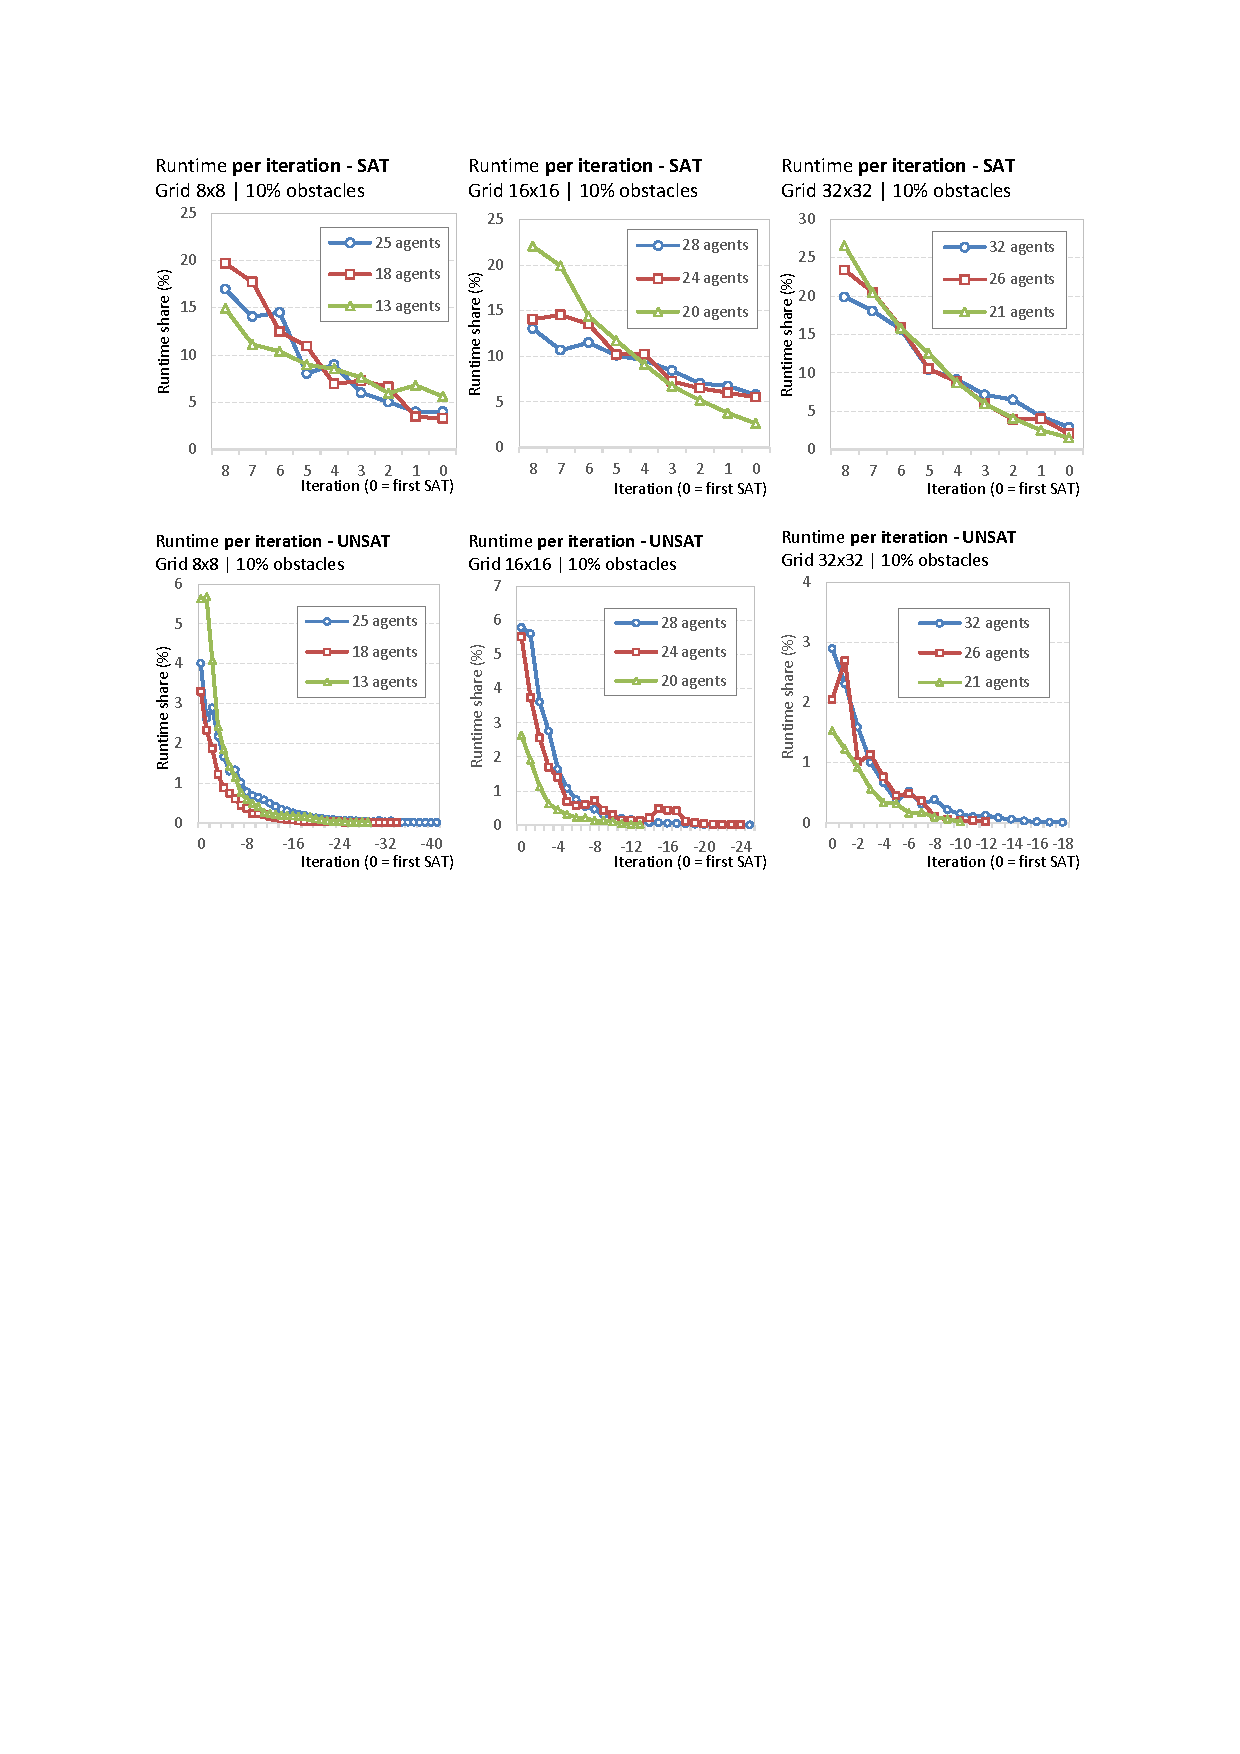
\includegraphics[trim={2.5cm 15.0cm 2.5cm 2.6cm},clip,width=1.0\textwidth]{exprMI_iter_grids.pdf}
\vspace{-0.6cm}\caption{Runtime results for individual iterations in  $8{}\times{}8$, $16{}\times{}16$, and $32{}\times{}32$ grids. The satisfiable (top) and the unsatisfiable (bottom) phases are shown. Eight extra iterations in the satisfiable phase are evaluated. The ratio of the total runtime consumed by each iteration is shown. }
\label{figure-iter-grids}
\end{figure}

The horizontal axis shows iterations of $\xi$ ($\Delta$) indexed from the first satisfiable iteration that is assigned the index 0, iterations in the satisfiable phase are assigned positive indices while the unsatisfiable phase is assigned negative indices. The results for each grid/map are divided into separate plots for the satisfiable phase (upper plot) and for the unsatisfiable phase (lower plot). MDD-SAT runs for 8 extra iterations of $\xi$ ($\Delta$) above the first satisfiable one. The plots show the ratio of the total runtime consumed per iteration (the sum of runtimes in all iterations corresponds to $1.0$). The results are averaged through 10 random instances per each number of agents.

\begin{figure}[h]
\centering
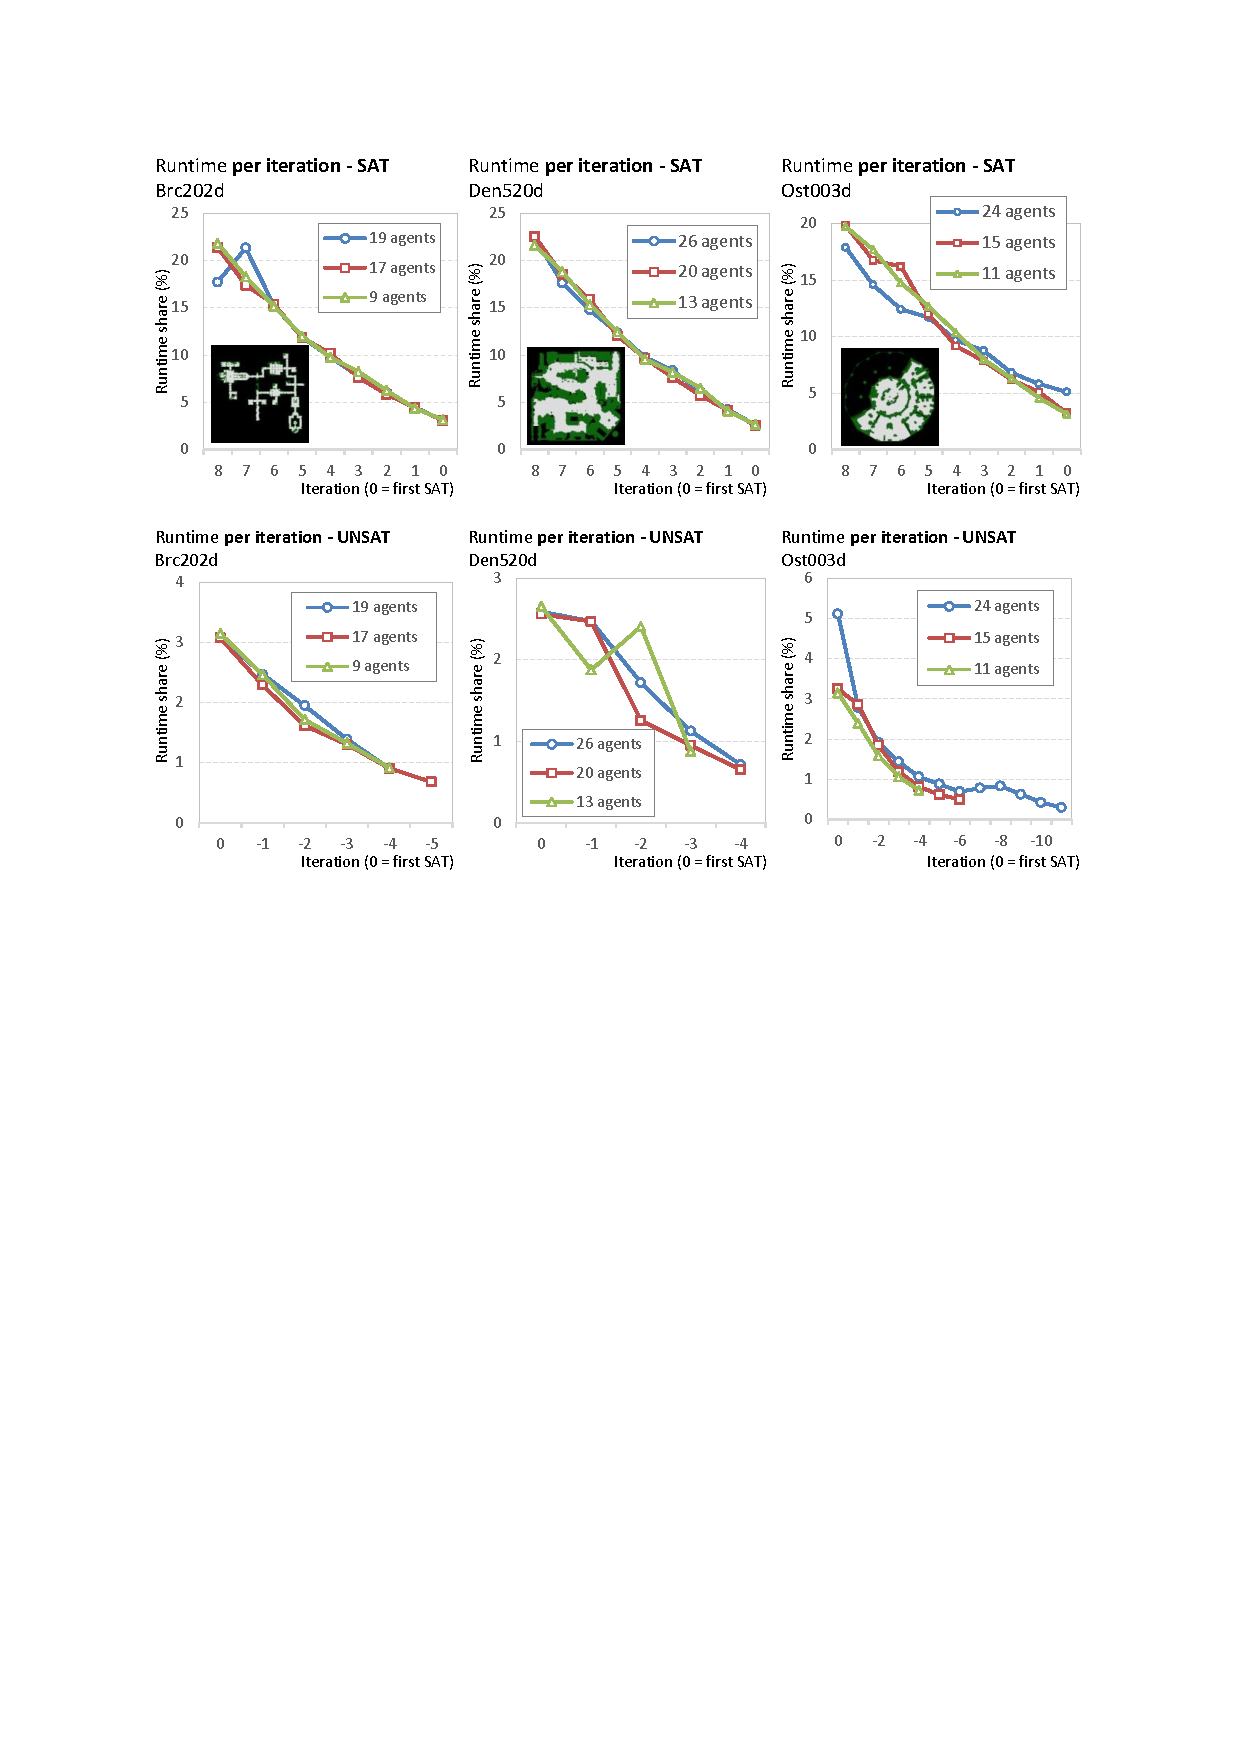
\includegraphics[trim={2.5cm 15.0cm 2.5cm 2.6cm},clip,width=1.0\textwidth]{exprMI_iter_maps.pdf}
\vspace{-0.6cm}\caption{Runtime results for individual iterations in DAO maps \texttt{brc202d},  \texttt{den520d}, and \texttt{ost003d}. The satisfiable (top) and the unsatisfiable (bottom) phases are shown. Eight extra iterations in the satisfiable phase are evaluated. The ratio of the total runtime consumed by each iteration is shown.}
\label{figure-iter-maps}
\end{figure}

The results show that in small grids the runtime in the unsatisfiable case exhibits an exponential growth as getting closer to the first satisfiable formula (lower three plots in Figure \ref{figure-iter-grids}). After reaching the satisfiable phase the growth of rutimes is slower (upper three plots in Figure \ref{figure-iter-grids}). Similar results can be observed for large maps in Figure \ref{figure-iter-maps} though there the hypothesized behaviour is less pronounced.

This result experimentally verifies that the adopted incremental scheme is suitable as answering by the SAT solver the formulae around the boundary between the unsatisfiable and the satisfiable case is as hard as to answer all formulae in the unsatisfiable phase. Different strategies that attempt to go further in the satisfiable phase could only add significant computational effort even by single consultation with the SAT solver.


\subsubsection{Evaluation of Time Expansions}
\label{sec:expansions}

The number of MDD time expansions (denoted $\mu$ in the pseudo-codes) needed to find an optimal solution may either be greater than or equal to the makespan of that optimal solution. Intuitively said the MDD-SAT algorithm needs to permit that all the extra cost when $\Delta$ is consumed by a single agent, resulting in the makespan of $\mu_0+\Delta$. Since the runtime of our algorithm depends strongly on the number of time expansions, the gap between the number of time expansions and the makespan of the optimal solution suggests that suboptimal solutions (or even optimal solutions without proving they are optimal) may be found faster by having fewer time expansions.

Figures \ref{figure-make-expand-grids_100} and \ref{figure-make-expand-maps_100} plot the difference between the optimal makespan and number of time expansions done by our algorithm, for different MAPF configurations (number of agents, grid/map type). Results are aggregated for 10 random instances in a box-plot showing the median, the 1st and the 3rd quartil, maximum and minimum, and outliers.

As can be seen, the gap grows as we increase the number of agents. This trend is especially visible in grids. This suggests that a suboptimal variant of our algorithm in which we relax the cost bound constraint may be able to find valid solutions much faster for harder problems. We explore this option in Section~\ref{sec:suboptimal}. 

\begin{figure}[h]
\centering
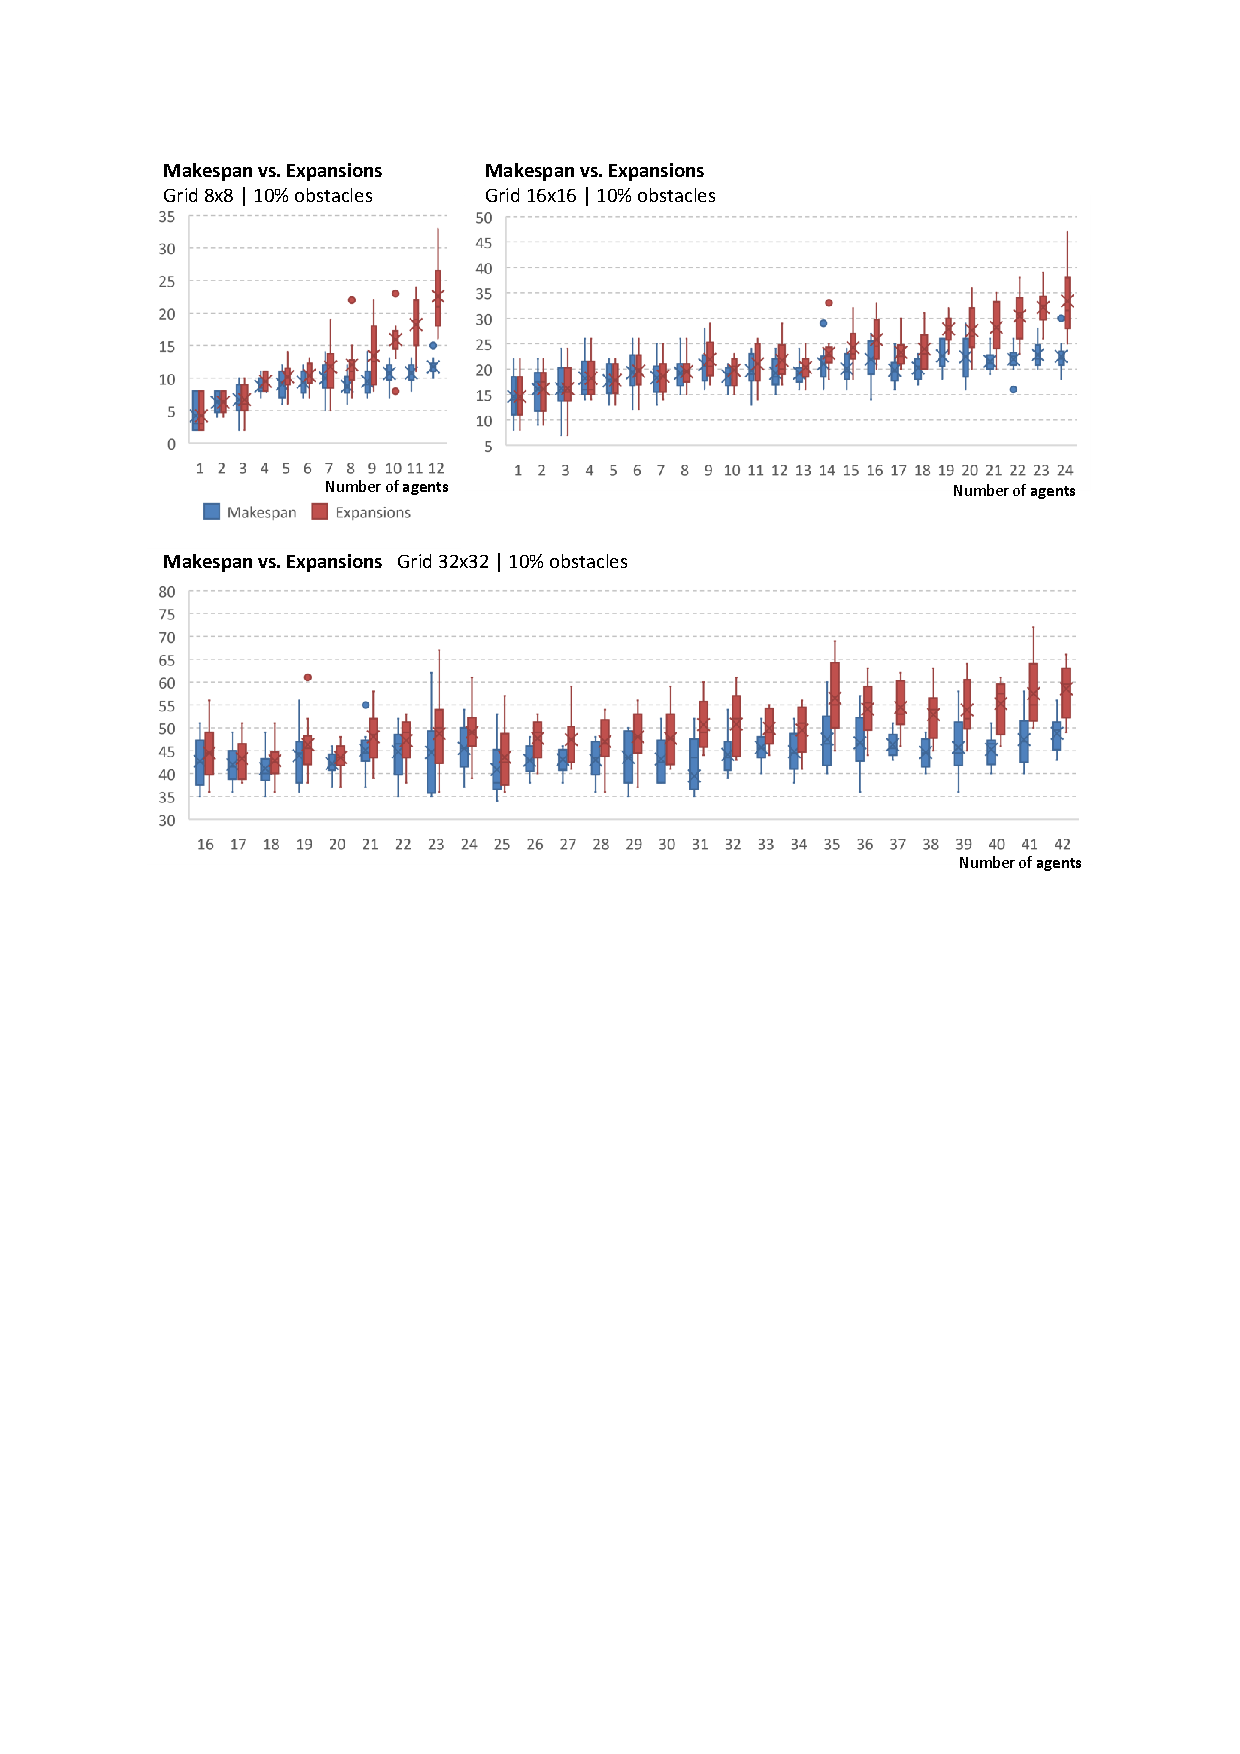
\includegraphics[trim={2.5cm 14cm 2.5cm 2.5cm},clip,width=1.0\textwidth]{expr_grids-make-expand_100.pdf}
\vspace{-0.6cm}\caption{Comparison of computed makespan in sum-of-costs optimal solutions and the number of time expansions of MDDs in $8{}\times{}8$, $16{}\times{}16$, and $32{}\times{}32$ grids.}
\label{figure-make-expand-grids_100}
\end{figure}

\begin{figure}[h]
\centering
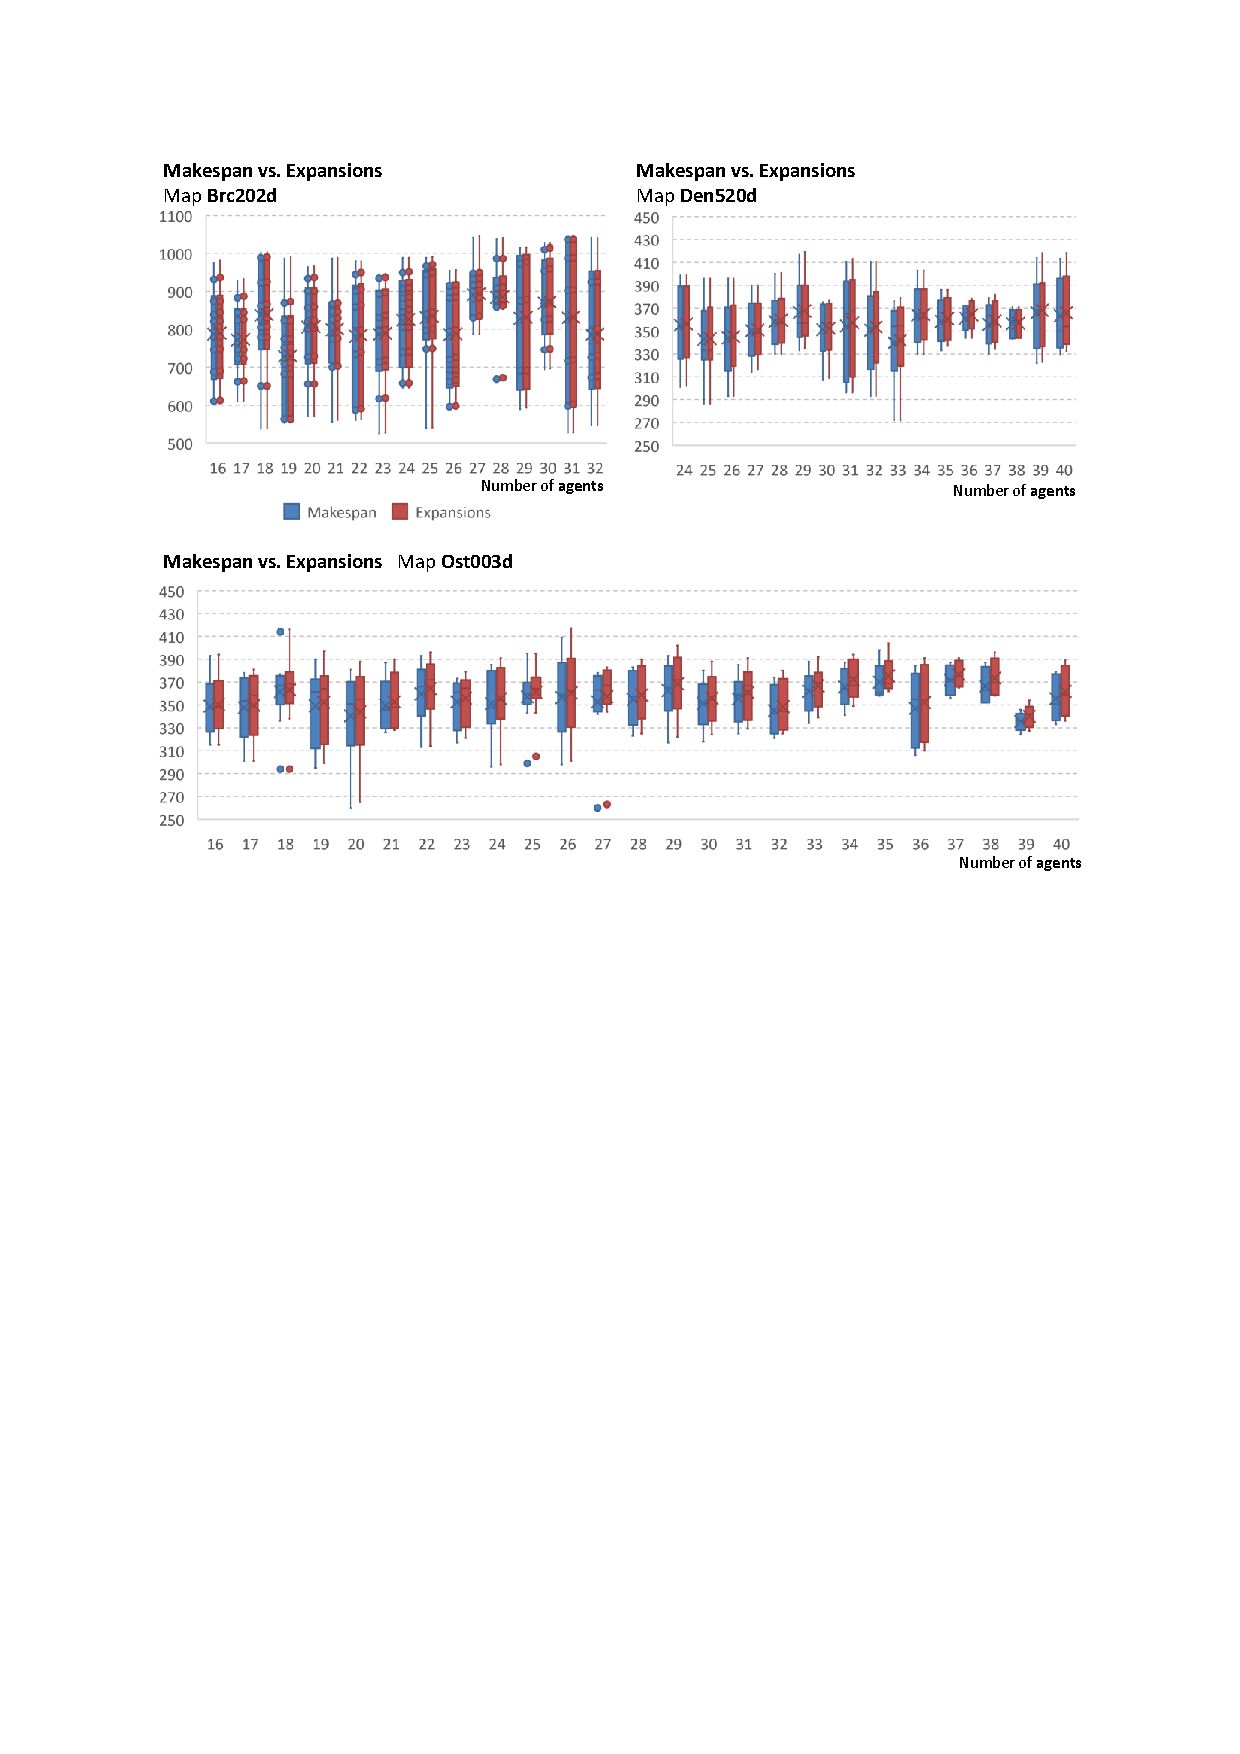
\includegraphics[trim={2.5cm 14cm 2.5cm 2.7cm},clip,width=1.0\textwidth]{expr_maps-make-expand_100.pdf}
\vspace{-0.6cm}\caption{Comparison of computed makespan in sum-of-costs optimal solutions and the number of time expansions of MDDs in DAO maps \texttt{brc202d}, \texttt{den520d}, and \texttt{ost003d}.}
\label{figure-make-expand-maps_100}
\end{figure}

\subsubsection{Reflecting Advances of Recent SAT Solvers}

\begin{figure}[h]
\centering
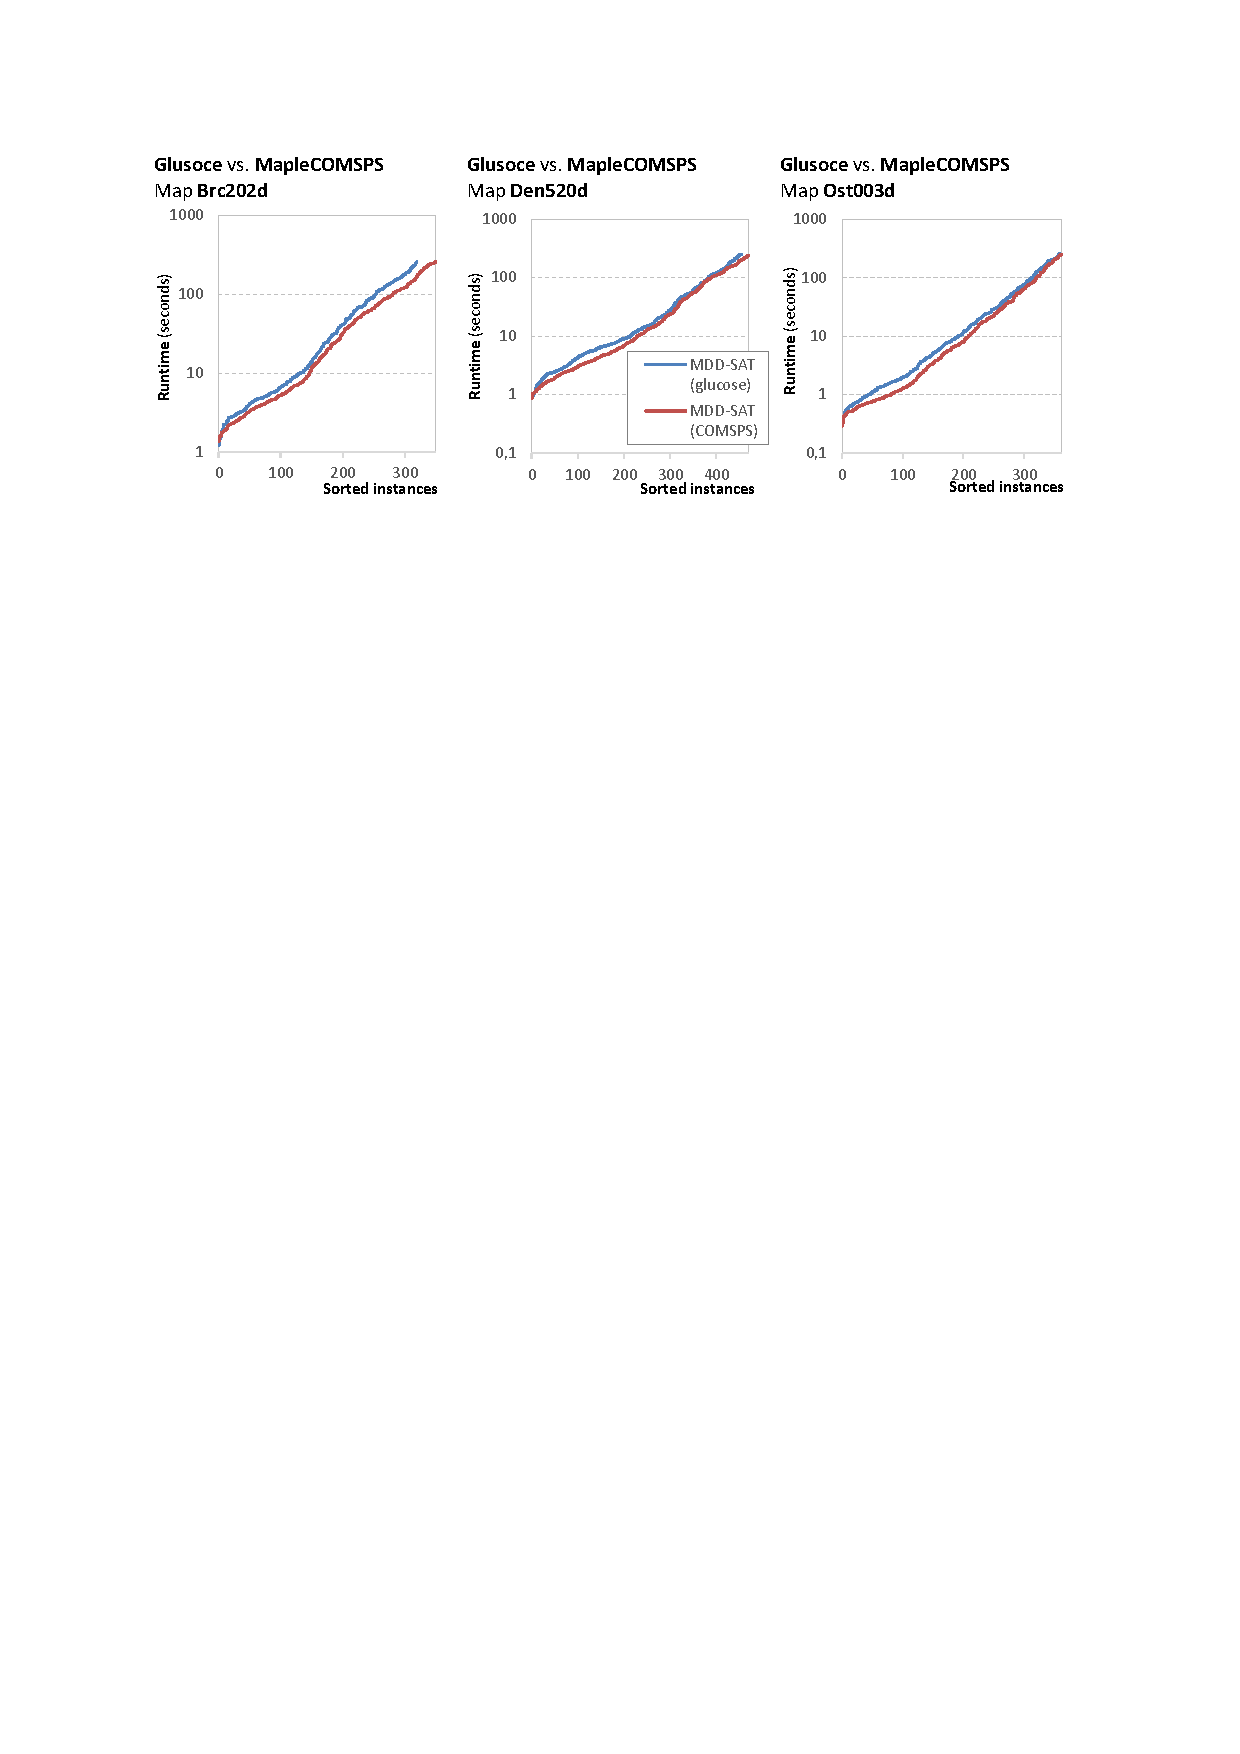
\includegraphics[trim={2.5cm 21.0cm 2.5cm 2.6cm},clip,width=\textwidth]{expr_maps_GLU-COM.pdf}
\vspace{-0.4cm}
\caption{Sorted runtimes of MDD-SAT with the Glucose SAT solver and MDD-SAT with the MapleCOMSPS for DAO maps \texttt{brc202d}, \texttt{den520d}, and \texttt{ost003d}.}
\label{expr_maps-GLU-COM}
\end{figure}

The major advantage of SAT-based solvers in general such as MDD-SAT is that they are modular and it is easy to exchange the SAT module for a newer one. The SAT-based solvers expected to perform better as the state of the art in SAT solving advances. In fact, in the course of writing the paper, a new SAT solver appeared, namely \texttt{MapleCOMSPS}~\cite{MAPLE_SAT_COMSPMS,DBLP:conf/sat/LiangOMTLG18}, that according to the results in recent SAT competitions outperforms the \texttt{Glucose} SAT solver \cite{DBLP:conf/aaai/BalyoHJ17}, originally used in MDD-SAT. Indeed, the integration of this new solver resulted in an improvement of MDD-SAT in some cases. 

To demonstrate this, we run MDD-SAT with the \texttt{MapleCOMSPS} SAT solver and compared it with MDD-SAT using the \texttt{Glucose} SAT solver (that is the SAT solver used in all the other experiments). We performed this comparison in a range of maps, including the $8{}\times{}8$, $16{}\times{}16$, and $32{}\times{}32$ grids with 10\% obstacles and all the DAO maps used in our experiments above. There were no significant difference in performance for the grids. However, we have observed a significant advantage for MDD-SAT with the \texttt{MapleCOMSPS} SAT solver on the DAO maps. These results are given in Figure~\ref{expr_maps-GLU-COM}, which follows the same format as in Figure~\ref{figure-ost003-sorted}. The results suggests that the \texttt{MapleCOMSPS} SAT solver can tackle large formulae resulting from solving MAPF on large DAO maps more efficiently than the \texttt{Glucose} SAT solver.


% \begin{figure}[h]
% \centering
% 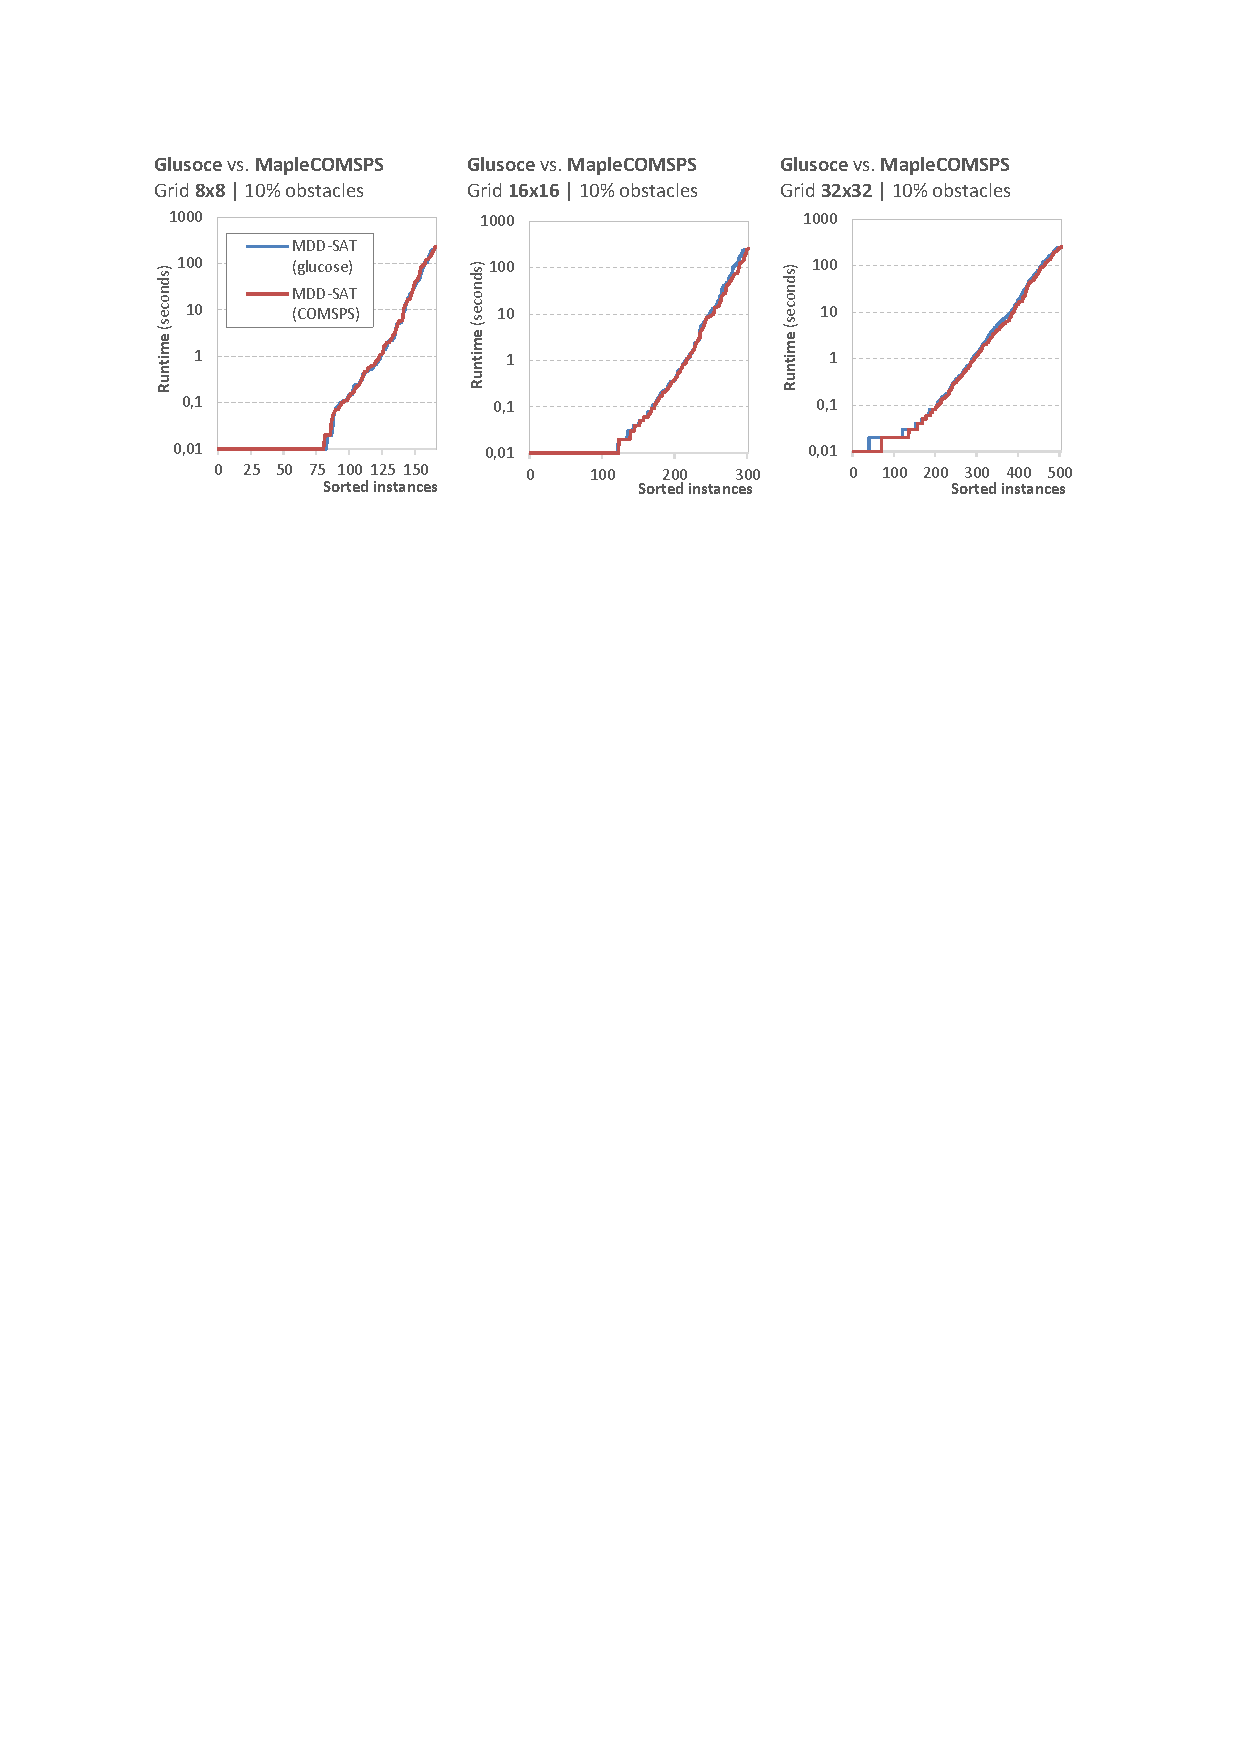
\includegraphics[trim={2.5cm 22.0cm 2.5cm 2.5cm},clip,width=\textwidth]{expr_grids_GLU-COM.pdf}
% \vspace{-0.4cm}
% \caption{Sorted runtimes of MDD-SAT with the Glucose SAT solver and MDD-SAT with the MapleCOMSPS for $8{}\times{}8$, $16{}\times{}16$, and $32{}\times{}32$ grids.}
% \label{expr_grids-GLU-COM}
% \end{figure}

\section{Independence Detection in SAT-Based Approach}

A successful method for increasing performance of MAPF solving algorithms is a technique called {\em independence detection} (ID). In this section, we describe how to integrate independence detection for MAPF \cite{DBLP:conf/aaai/Standley10,DBLP:conf/ijcai/StandleyK11} into MDD-SAT. We summarize here and extend the results originally published as conference papers \cite{DBLP:conf/icaart/SurynekSFB17,DBLP:conf/icaart/SurynekSFB17a}.

The main idea behind this technique is that the difficulty of optimal MAPF solving grows {\bf exponentially} with the number of agents. It would be ideal, if we could divide the problem into a series of smaller independent sub-problems, solve them independently, and merge solutions to the sub-problems to form a solution of the original problem. Having exponential complexity for the original instance such decomposition could lead to significant speed up.

More precisely, assume that the time complexity of solving the given MAPF problem with $k$ agents is $\mathcal{O}(2^k)$. Then the problem is decomposed into say two independent sub-problems with $k/2$ agents and these two sub-problems are solved separately taking time of $\mathcal{O}(2^{\frac{k}{2}}) +\mathcal{O}(2^{\frac{k}{2}}) = \mathcal{O}(2^\frac{k}{2})$. If the dividing phase and the final sub-solution merging phase have lower than exponential time complexity, for example polynomial in the number of agents, then the overall speed up could be $\mathcal{O}(2^{\frac{k}{2}})$-fold.

The important assumption that only some problems satisfy is the requirement of having independent sub-problems that can be solved separately. In MAPF fortunately, this is relatively common situation in sparse environments. Consider groups of agents in distant sub-graphs whose goals are located in the same sub-graph. Then it is unlikely that these groups will ever have chance to meet each other in an optimal solution. Hence optimal solution to the problem can be constructed as the union of optimal solutions for individual groups.

\subsubsection{Independence Detection Variants in Search-Based Solvers}

For completeness, we first give a detailed description of ID as it has been described by prior work in a search-based MAPF solver, namely A*~\cite{standley2010finding}. 
%Let us recall existing concepts of ID for MAPF in the context of A* algorithm. 
The basic approach, called {\em simple independence detection} (SID), divides agents into multiple groups. Initially, each agent is assigned into its own group (consisting of a single agent). The algorithm regards each of these groups as independent sub-problem and searches for optimal MAPF solutions of individual groups. Solutions obtained from this independent solving are then checked for conflicts. For every pair of solutions, it checks if a collision between agents from different solutions/groups occurs.

If a collision occurs then respective groups are merged together and new optimal solution is found for the merged group. The process is repeated until there are no conflicts between group solutions. If there are no conflicting solutions, the solutions for individual groups can be merged together to from a single solution of the original problem.

Merging groups together after detecting a conflict could quickly lead to large groups (an extreme case is having single group consisting of all agents). The SID approach can be further improved by avoiding group merging if possible.

Generally, there exists more than one optimal path of each agent or more than one optimal MAPF solutions for a group of agents. The SID technique, however, ignores these alternative paths and solutions. The improvement of SID known as {\em independence detection} (ID) is as follows.

\begin{algorithm}[h]
\begin{footnotesize}
\SetKwBlock{NRICL}{Solve-MAPF-A*+ID($\Sigma=(G=(V,E),A,\alpha_0,\alpha_+)$)}{end} \NRICL{
      \For {each $a_i \in A$}{
      	    $G_i \gets \{a_i\}$\\
      	    $\mathit{\pi}(G_i) \gets$plan-MAPF-A*$(G=(V,E),G_i,\alpha_0,\alpha_+)$\\
 	}
	\While {$G_i$ and $G_j$ exist such that $\mathit{\pi}(G_i)$ and $\mathit{\pi}(G_j)$ conflict}{
	    \If {$\mathit{\pi}(G_i)$ and $\mathit{\pi}(G_j)$ not conflicted before}{
              $\mathit{\pi}'(G_i) \gets$replan-MAPF-A*$(G=(V,E),G_i,\alpha_0,\alpha_+,\pi, G_j)$\\
              \If{$\mathit{\pi}'(G_i) =$Fail}{
                  $\mathit{\pi}(G_j) \gets$replan-MAPF-A*$(G=(V,E),G_j,\alpha_0,\alpha_+,\pi, G_i)$\\
              }
              \Else{
                $\mathit{\pi}(G_i) \gets \mathit{\pi}'(G_i)$\\
              }
	    }
	    \Else{
	        $\mathit{\pi}(G_i) \gets$ Fail\\
	        $\mathit{\pi}(G_j) \gets$Fail\\
	    }
	    \If{$\mathit{\pi}(G_i)=\;$Fail or $\mathit{\pi}(G_j)=\;$Fail}{
	        $G_i \gets G_i \cup G_j$\\
	        $G_j \gets \emptyset$\\
	        $\mathit{\pi}(G_i) \gets$plan-MAPF-A*$(G=(V,E),G_i,\alpha_0,\alpha_+)$\\
	    }
	}
       \Return $\pi$\\
}
\caption{MAPF solving algorithm based on independence detection technique. Planning for groups is always done to have the least number of conflicts with respect to conflict avoidance table.}
\label{alg-A-ID}
\end{footnotesize}
\end{algorithm}

Assume two conflicting groups of agents $G_i$ and $G_j$. We try to avoid merging $G_i$ with $G_j$ via re-planning. First, we try to re-plan for $G_i$ so that the new solution has the same cost but conflicts with $G_j$ are forbidden. If no such solution exists, we try to replan for $G_j$. If re-planning for $G_j$ fails as well, then we merge $G_i$ and $G_j$ into a new group. After successful re-planning, the new MAPF solution for the group needs to be evaluated with every other group again. This could lead to infinite cycle. Therefore, if two groups were in conflict before, we merge them without trying to replan.

The original ID technique was used in combination with the A* algorithm that was used for path finding (searching for solutions for individual groups). The independence detection can be further supported at the level of path finding. The A* algorithm can be fine tuned to prefer paths that create as few as possible conflicts with other groups that have their solutions finished.

The MAPF solving algorithm based on A* and ID is listed using pseudo-code as Algorithm~\ref{alg-A-ID}. Let us note that initial paths for a group are found while ignoring all agents outside the group (lines 4 and 13) but when re-planning for a group we take into account existing paths for other groups including the group towards which we are trying to resolve conflicts (lines 7 and 9).  When A* has a choice between several nodes with the same minimum $f()$ cost in the re-planning phase, the one with the least amount of conflicts with respect to other group's paths is expanded first. This technique, which is also known as using a Conflict Avoidance Table (CAT), yields an optimal solution that has the minimal number of conflicts with other groups. In other words, the re-planning phase strictly avoids paths of the other group in conflicting pair but also prefers avoiding paths of other groups though this is a preference only (not a strict constraint).

Both SID and ID do not solve MAPF on their own, they only divide the problem into smaller sub-problems that are solved by any possible MAPF algorithms. Thus, ID and SID are general frameworks which can be executed on top of any MAPF solver.

\subsubsection{Integration of Independence Detection into MDD-SAT}

Next, we describe how ID can be applied in SAT based MAPF solvers. The common feature of SAT based MAPF solvers, MDD-SAT included, is that they consider the entire MAPF instance as a whole which can limit their scalability for large instances.

\begin{wrapfigure}{l}{0.5\textwidth}
\begin{center}
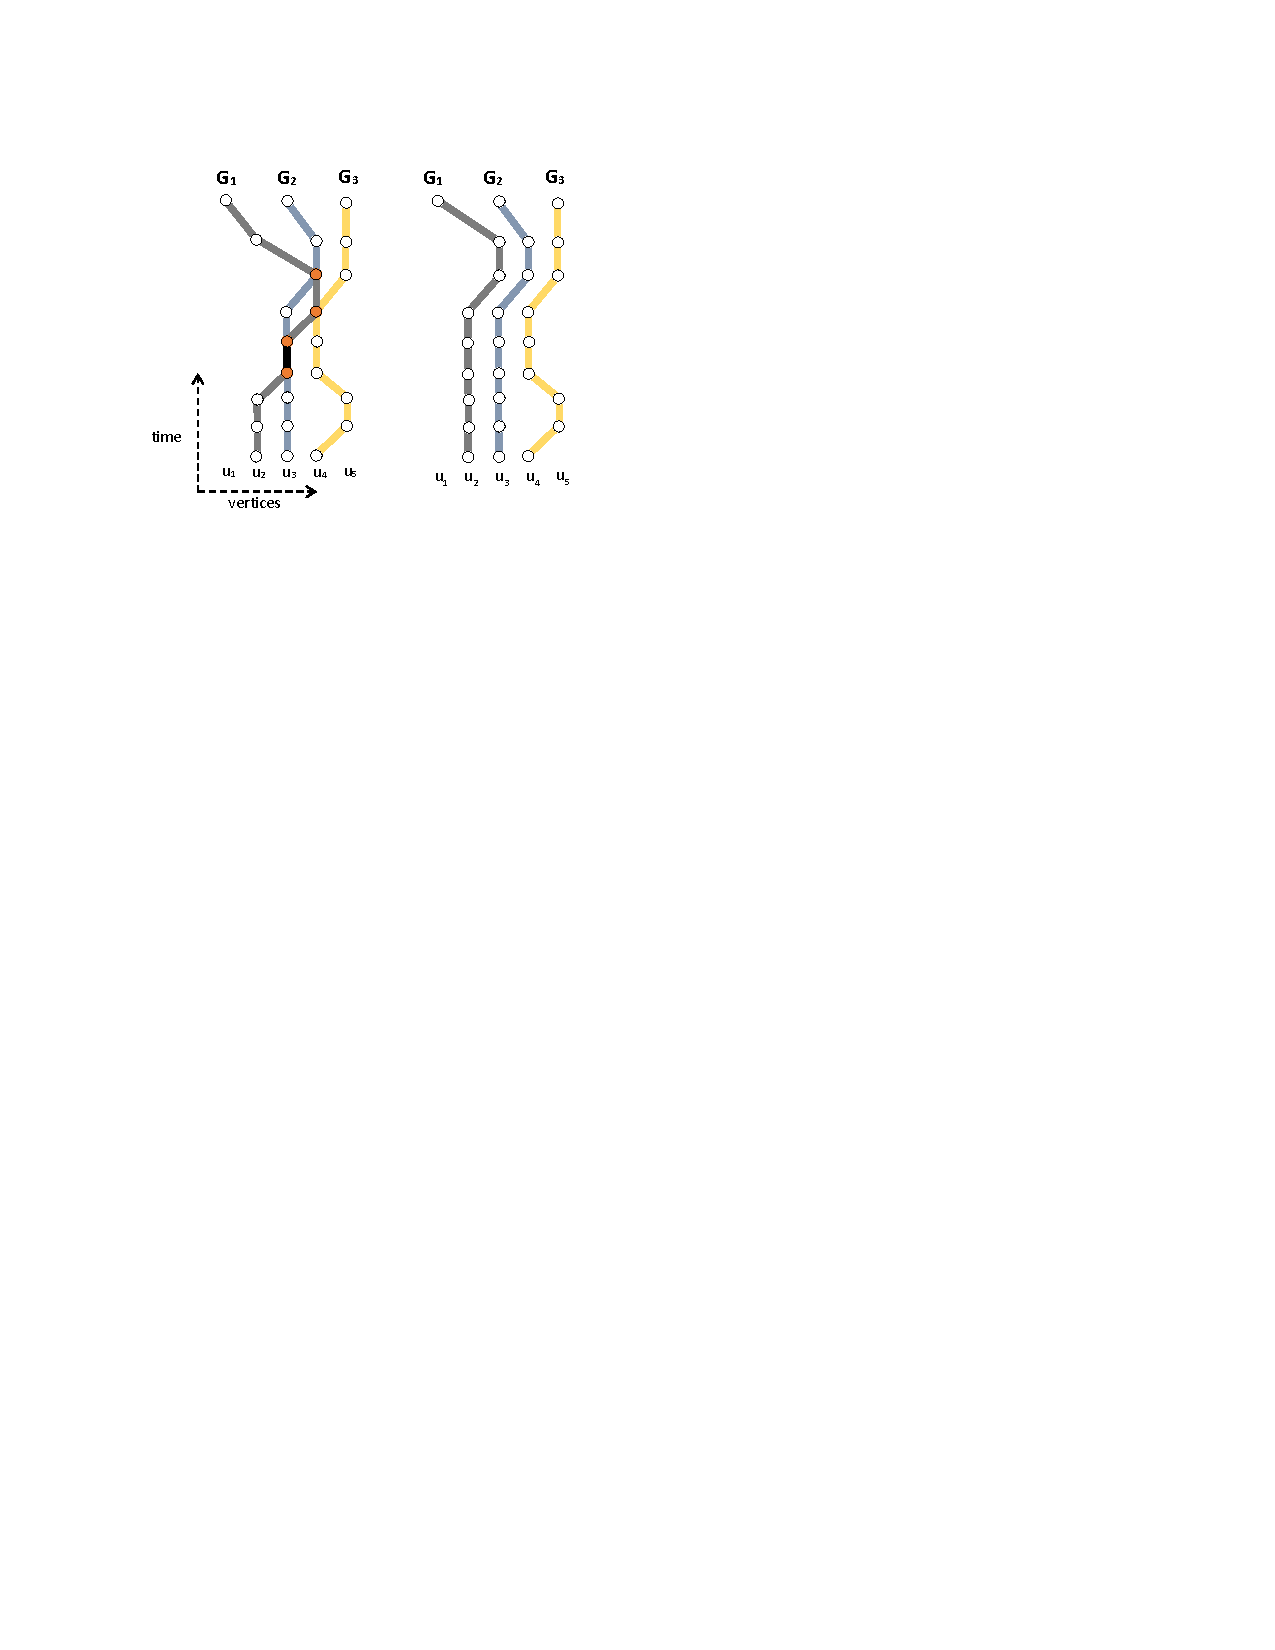
\includegraphics[trim={2.5cm 19.2cm 3.0cm 2.7cm},clip,width=1.0\textwidth]{fig_ID.pdf}
\end{center}
\caption{Groups $G_1$ conflicts with groups $G_2$ and $G_3$ (left). After replanning $G_1$ independent solutions for $G_1$, $G_2$, and $G_3$ can be merged together. } \label{figure-ID}
\end{wrapfigure}

With large instances and many agents, MDD-SAT will eventually encounter a formula of prohibitive size even with the use of MDDs. In contrast to this, search-based solvers often use some variant of ID to further mitigate the size of the instance needed to be tackled at once.

The logical step is hence to integrate a variant of ID into MDD-SAT. The SAT-based approach however requires modification of the original ID since in the propositional formula it is not possible to express preference that individual paths of groups of agents should avoid the occupied positions by other groups. In the yes/no SAT environment we either manage to avoid occupied positions or not while in the negative case there is no tool how to control the number of conflicts. In other words, in our implementation of ID there we do not use a CAT to bias the paths returned for the agents. 

The SAT-based version of ID works in a similar way to the original version but instead of resolving conflicts between a pair of conflicting groups $G_i$ and $G_j$ it resolves conflict of group $G_i$ with all other groups. If this attempt is successful, $G_i$ is independent on others and the process can continue with resolving conflicts between remaining groups (see Figure \ref{figure-ID} where $G_1$ has been made independent of $G_2$ and $G_3$). If the attempt to resolve conflicts between $G_i$ and $G_j$ by making $G_i$ independent of all other groups fails, the same is tried for $G_j$. If the attempt for $G_j$ fails too, then $G_i$ and $G_j$ are merged. The pseudo-code of the process is shown in Algorithm \ref{alg-MDD-SAT-ID}.

In contrast to the original ID we strictly require avoidance with respect to other groups. This is technically done by omitting the conflicting vertices in the MDD. More precisely, when planning for group $G_i$ (line 7) we first build MDDs for agents $a \in G_i$. For each node in MDD we need to check whether it conflicts with paths for agents in the remaining groups.

Assume node $u_j^t$ in MDD for agent $a$ corresponding to $u_j \in V$ and time step $t$. Several cases need to be distinguished \footnote{Depending on the variant of MAPF the cases can be different. Here we follow the move-to-unoccupied variant where agents move to vacant vertices.}:

\begin{itemize}
\item Case {\bf (i)} occurs if vertex $u_j$ is occupied by some agent $a' \in A \setminus G_i$ at time step $t$ (that is, $\pi(a')[t] = u_j$; where $\pi(a')[t]$ denotes the $t$-th vertex of path for agent $a'$). This situation corresponds to violation of the constraint that at most one agent reside in each vertex. If this is detected then $u_j^t$ is omitted from given MDD for agent $a$.
\item Case {\bf (ii)} occurs if vertex $u_j$ was occupied by some agent $a' \in A \setminus G_i$ at time step $t-1$ which corresponds to violation of the constraint that agent can enter a vacant vertex only. Again in such case using $u_j$ at time step $t$ is forbidden for agent $a$ and thus $u_j^t$ is omitted from MDD.
\end{itemize}

The rest is automatically expressed by the semantics of the formula. Occupied vertices omitted from MDD are not represented in the formula. Hence the SAT solver cannot use these vertices for planning agents' paths. If the SAT solver succeeds with path finding then resulting paths automatically avoid missing vertices and resulting paths do not conflict with paths of other groups.

The resulting algorithm is called MDD-SAT+ID. The algorithm returns sum-of-costs optimal solutions for solvable MAPF instances. The optimality guarantees are a direct consequence of properties of ID. The ID technique can be also used with the makespan-optimal version of MDD-SAT.
	
\begin{algorithm}[h]
\begin{footnotesize}
\SetKwBlock{NRICL}{Solve-MAPF-SAT$_{SOC}$+ID($\Sigma=(G=(V,E),A,\alpha_0,\alpha_+)$)}{end} \NRICL{
      \For {each $a_i \in A$}{
      	    $G_i \gets \{a_i\}$\\
      	    $\mathit{\pi}(G_i) \gets$Solve-MAPF-SAT$_{SOC}(G=(V,E),G_i,\alpha_0,\alpha_+)$\\
 	}
	\While {$G_i$ and $G_j$ exist such that $\mathit{\pi}(G_i)$ and $\mathit{\pi}(G_j)$ conflict}{
	    \If {$\mathit{\pi}(G_i)$ and $\mathit{\pi}(G_j)$ not conflicted before}{
              $\mathit{\pi}'(G_i) \gets$reSolve-MAPF-SAT$_{SOC}(G=(V,E),G_i,\alpha_0,\alpha_+,\pi)$\\
              \If{$\mathit{\pi}(G_i) =$Fail}{
                  $\mathit{\pi}(G_j)\gets$reSolve-MAPF-SAT$_{SOC}(G=(V,E),G_j,\alpha_0,\alpha_+,\pi)$\\
              }
              \Else{
                $\mathit{\pi}(G_i) \gets \mathit{\pi}'(G_i)$\\
              }
	    }
	    \Else{
	        $\mathit{\pi}(G_i) \gets$ Fail\\
	        $\mathit{\pi}(G_j) \gets$Fail\\
	    }
	    \If{$\mathit{\pi}(G_i)=\;$Fail or $\mathit{\pi}(G_j)=\;$Fail}{
	        $G_i \gets G_i \cup G_j$\\
	        $G_j \gets \emptyset$\\
	        $\mathit{\pi}(G_i) \gets$Solve-MAPF-SAT$_{SOC}(G=(V,E),G_i,\alpha_0,\alpha_+)$\\
	    }
	}
       \Return $\pi$\\
}
\caption{Independence detection in the sum-of-cost optimal SAT-based solver MDD-SAT. Conflict avoidance is strictly required.}
\label{alg-MDD-SAT-ID}
\end{footnotesize}
\end{algorithm}

\subsection{Experimental Results for MDD-SAT with Independence Detection}

\begin{figure}[h]
\centering
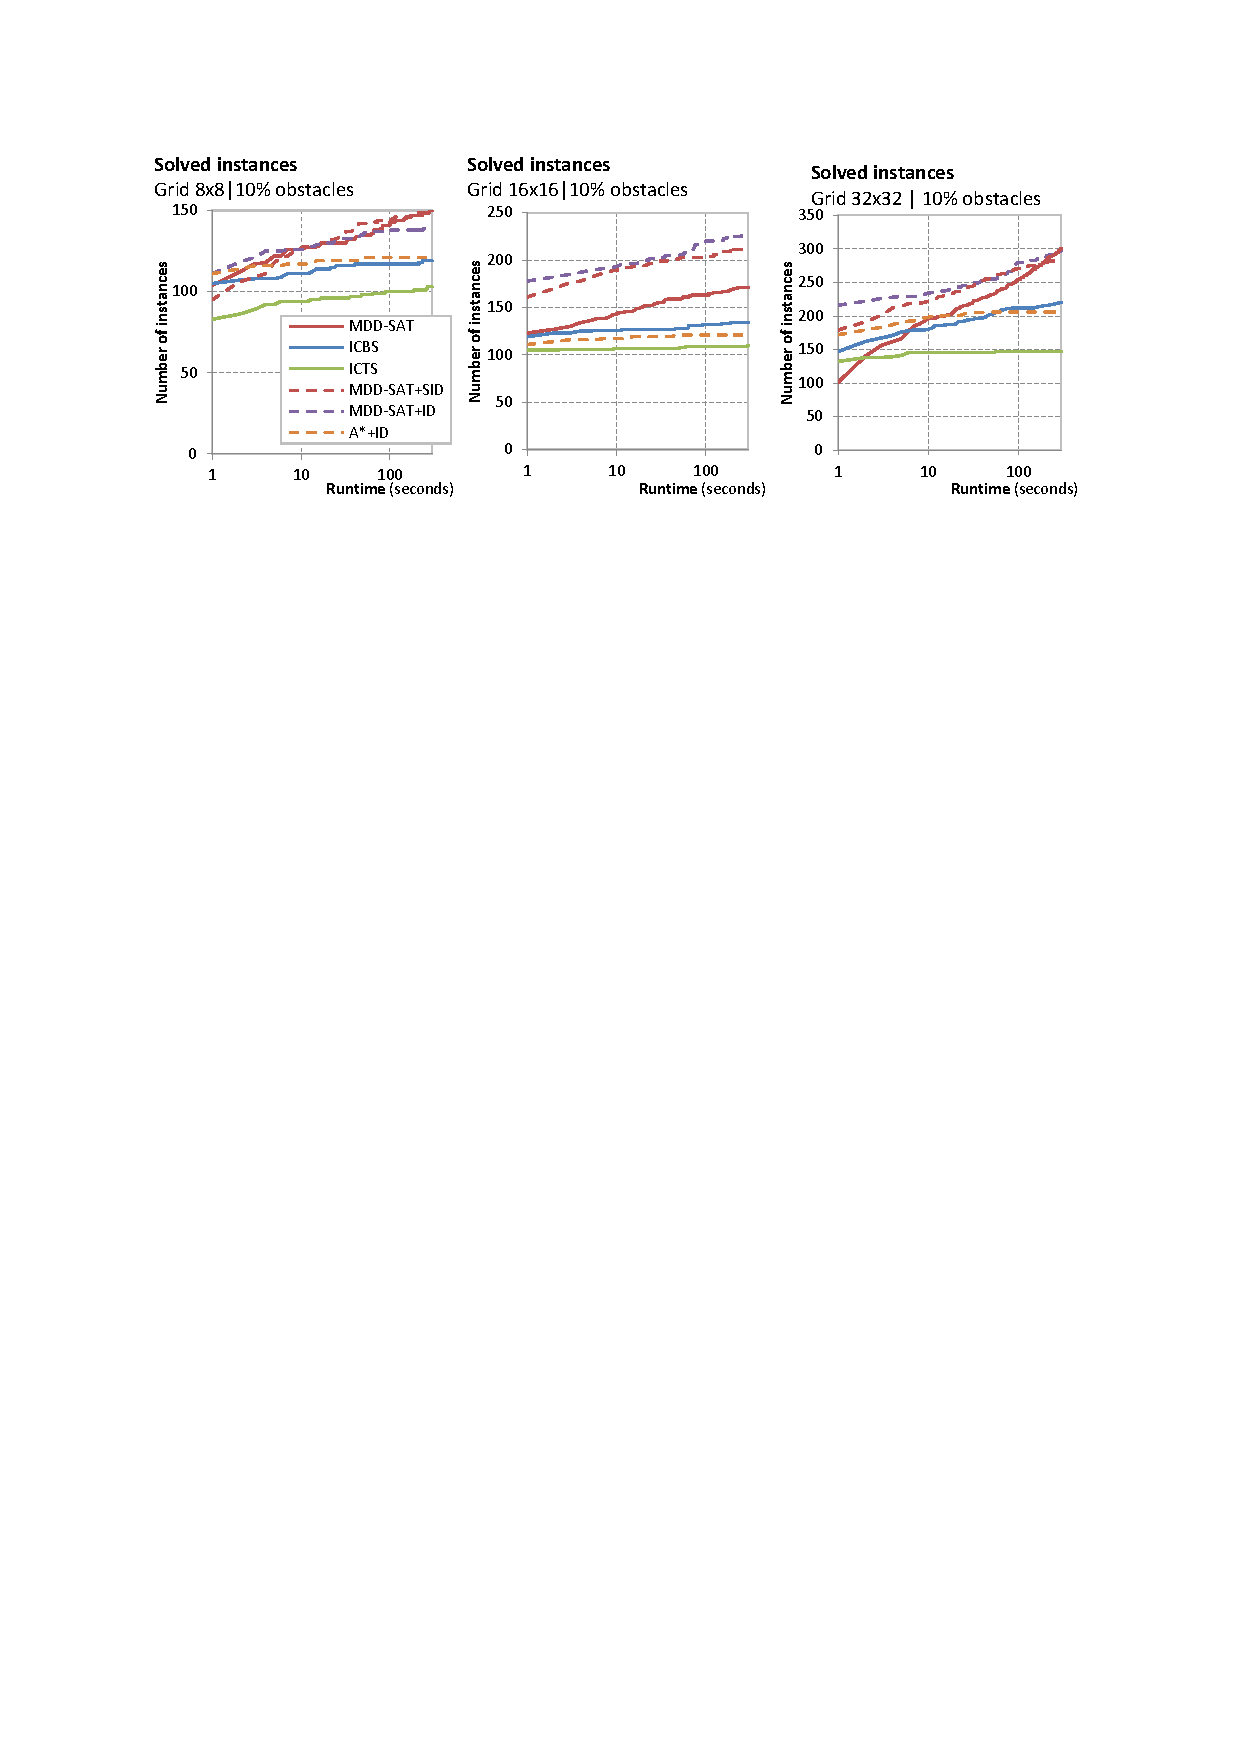
\includegraphics[trim={2.5cm 21.0cm 2.5cm 2.5cm},clip,width=\textwidth]{expr-id_grids-num-solved.pdf}
\vspace{-0.4cm}
\caption{Evaluation of ID and SID integrated in MDD-SAT - the number of solvable instances in $8{}\times{}8$, $16{}\times{}16$, and $32{}\times{}32$ grids as a function of the time limit (the horizontal runtime axis uses logarithmic scale).}
\label{expr-id_grids-num-solved}
\end{figure}

\begin{figure}[h]
\centering
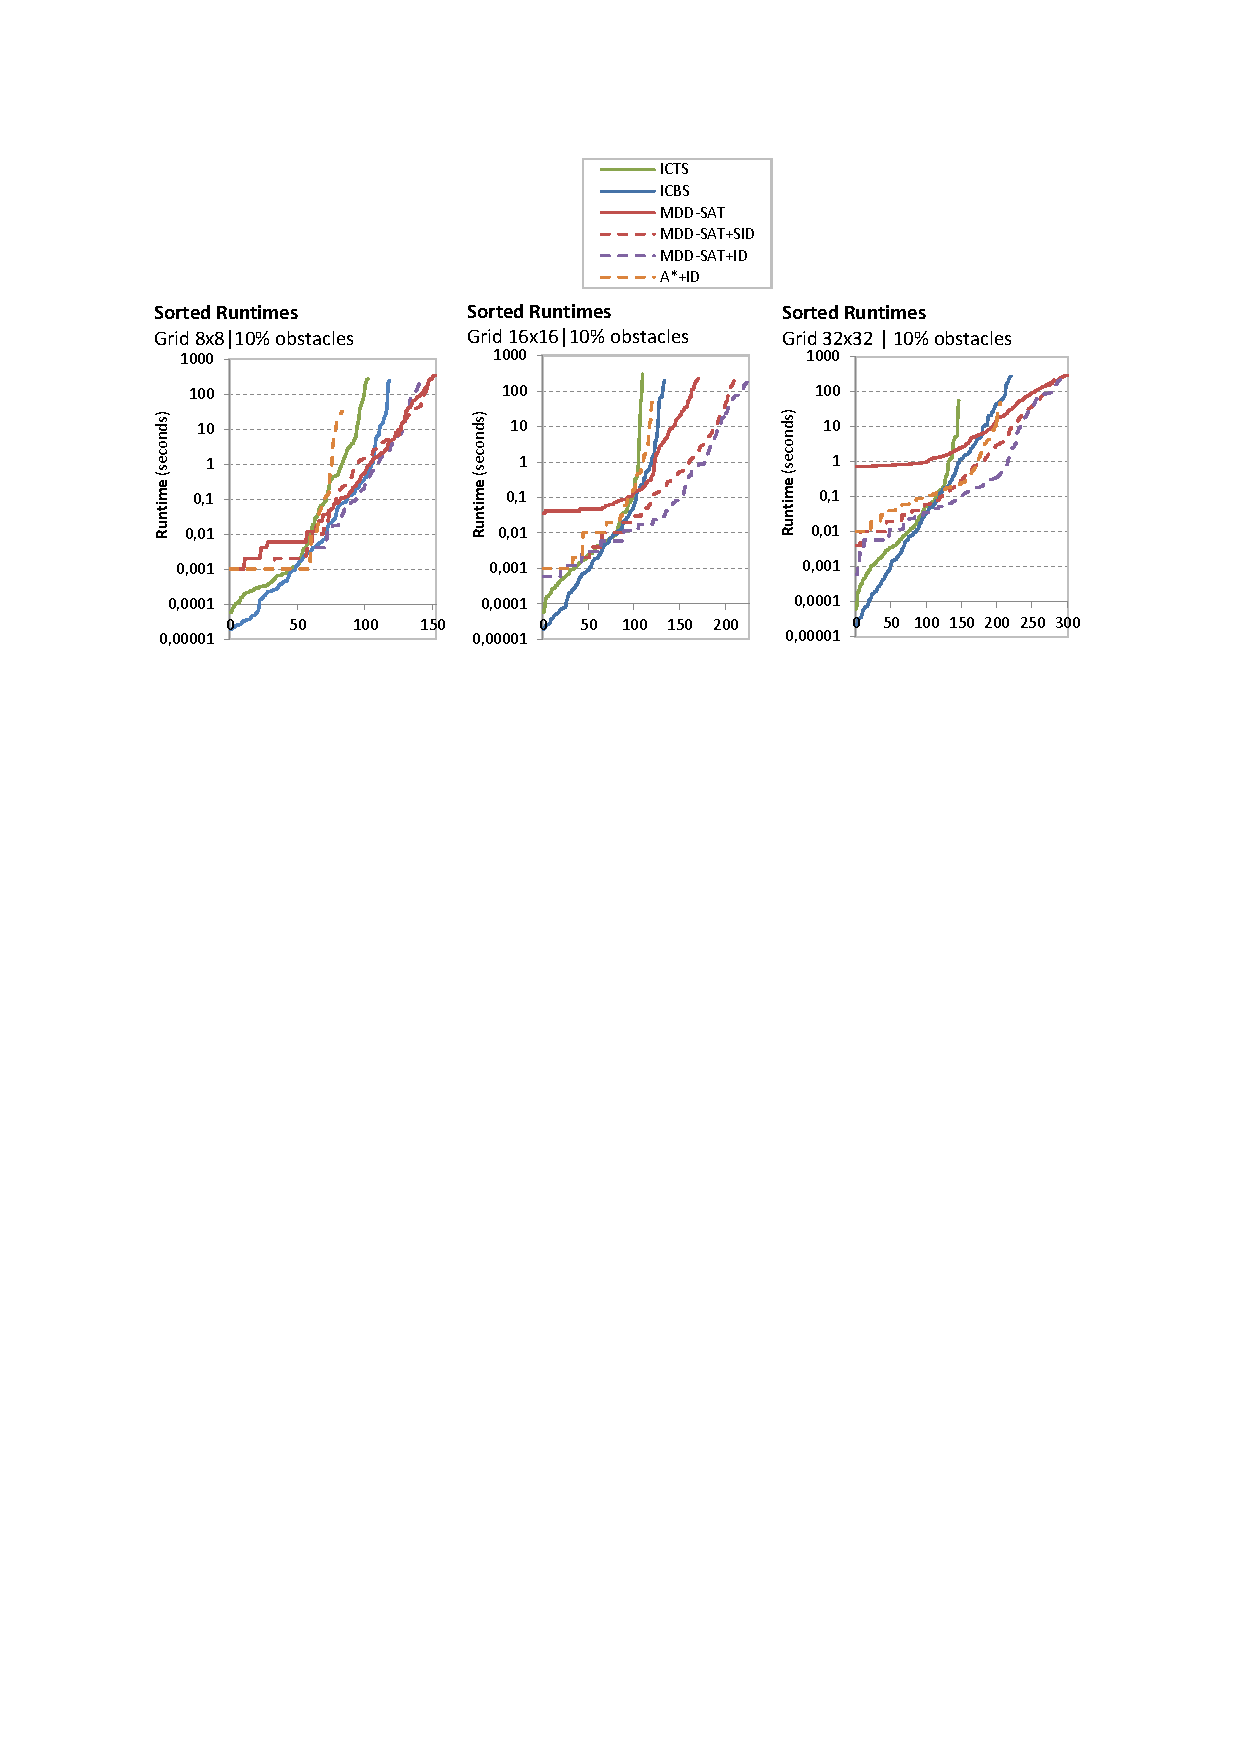
\includegraphics[trim={2.5cm 18.5cm 2.5cm 2.6cm},clip,width=\textwidth]{expr-id_grids-sorted.pdf}
\vspace{-0.4cm}
\caption{Evaluation of ID and SID integrated in MDD-SAT - sorted runtimes for $8{}\times{}8$, $16{}\times{}16$, and $32{}\times{}32$ grids (the horizontal axis corresponds to instances sorted differently for each tested algorithm).}
\label{expr-id_grids-sorted}
\end{figure}

We followed the same pattern in experiments for ID as in previous sections. Experiments were done on small 4-connected grids with obstacles and on large DAO maps. We implemented extensions of MDD-SAT using both simple independence detection (the solver denoted MDD-SAT+SID) and MDD-SAT with a independence detection (denoted MDD-SAT+ID). The implementation extends previous C++ implementation of MDD-SAT. The SID version only replans the conflicting group against the single group with which the conflict has been detected while other groups are ignored. We implement MDD-SAT+SID for having a reference base-line variant of independence detection. MDD-SAT+SID is expected to perform worse than MDD-SAT+ID where re-planning of conflicting group is done with respect to all remaining groups. MDD-SAT was also included in comparison too to see what is the benefit of ID in relation to its overhead. In addition to this, we included an implementation of Algorithm \ref{alg-A-ID} referred to as A*+ID in the plots. A*+ID implements operator decomposition \textsc{Od} in the A*-based search for non-conflicting paths (procedures plan-MAPF-A* and replan-MAPF-A*), hence A*+ID corresponds to Standley's \textsc{Od+Id} \cite{standley2010finding}.

In all tests we used time limit of 300 seconds. Testing instances for both the small grids and large DAO maps are identical to those used in previous tests. The hypothesis is that independence detection could be helpful in instances with few agents and lot of free space where there is a little interaction among agents and/or the environment provides opportunity to perform a collision free avoidance if necessary. On the other hand, detecting independence could represent a significant overhead on small densely populated maps where eventually all agents merge into one large group.

\subsubsection{Results of Independence Detection on Small Grids}

Results obtained with independence detection integrated in MDD-SAT on small grids of sizes $8{}\times{}8$, $16{}\times{}16$, and $32{}\times{}32$ are presented in Figures \ref{expr-id_grids-num-solved} and \ref{expr-id_grids-sorted}. We show two projections of the results: Figure \ref{expr-id_grids-num-solved} shows the number of successfully solved instances as a function of time. In Figure \ref{expr-id_grids-sorted} we take all instances that the selected solver managed to finish under the given time limit and sort them according to the ascending runtime.

The trends we can observe in the result supports the hypothesis. On $8{}\times{}8$, MDD-SAT+SID represents almost no significant improvement compared to MDD-SAT. MDD-SAT+ID even shows worsening in harder instances (needing longer runtime) compared to MDD-SAT. In easy instances we can observe that ID contributes to some minor improvement but SID does the opposite. We can attribute this behavior to the situation where agents do interact so collision avoidance is needed but there is enough free space at the same time to plan collision avoidance successfully (the ID case) but there is no abundance of free space so SID often hits some other group after re-planning.

In larger girds, $16{}\times{}16$, and $32{}\times{}32$ results suggest that different effect takes places. We can observe two significant patterns: (i) there is a consistent significant benefit of using both SID and ID across tested instances while the improvement decreases towards harder instances containing more agents, (ii) in instances of medium difficulty ID provides better results than SID.

The explanation for pattern (i) is that larger free space gives opportunity to independence detection to actually find independent groups of agents and finish searching with relatively small groups (small independent sub-problems). The region where pattern (ii) can be observed corresponds to the situation where we have enough free space for avoidance between groups but such free space is not abundant so all groups need to be carefully taken into account (like in the ID case) since otherwise some other group may be hit by the re-planned group (the SID case).

\begin{figure}[h]
\centering
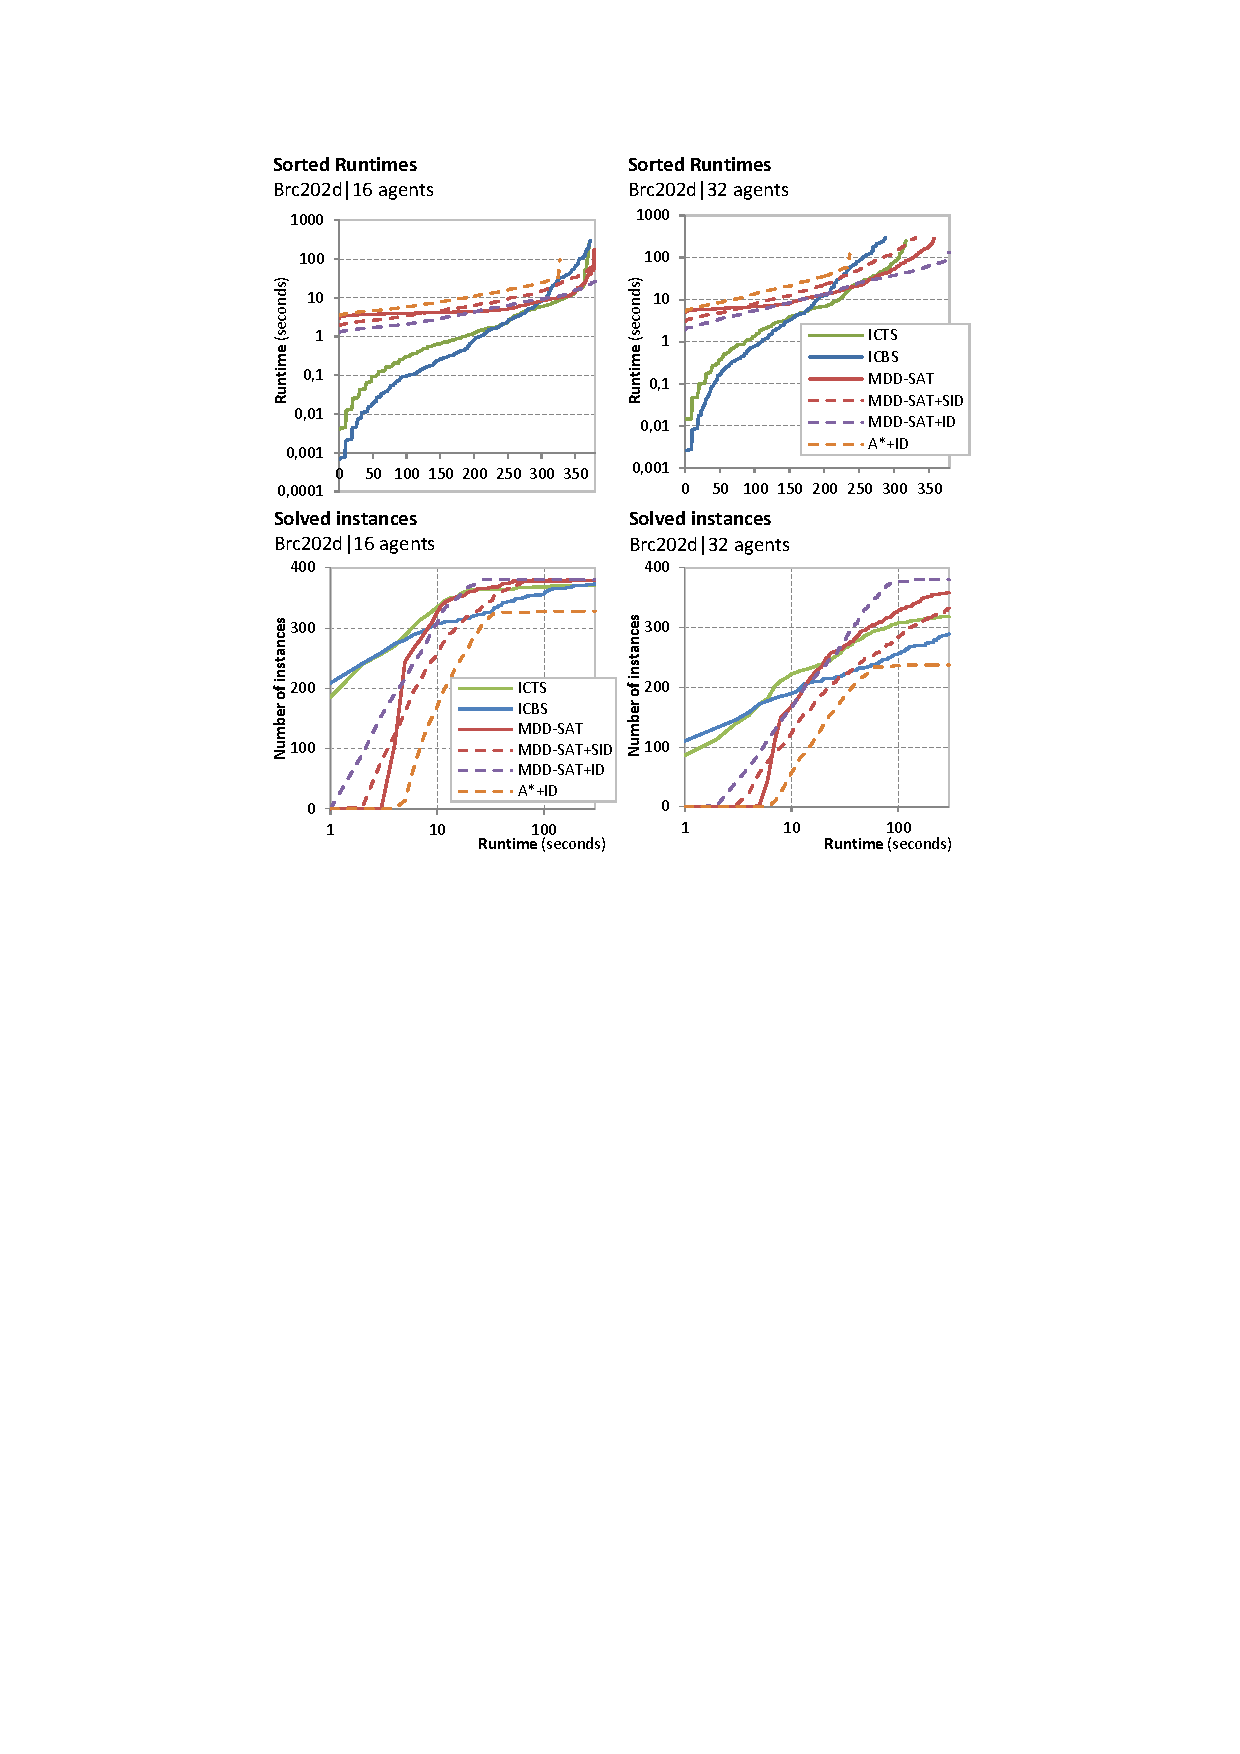
\includegraphics[trim={2.5cm 15.0cm 2.5cm 2.5cm},clip,width=1.0\textwidth]{expr-id_brc202_sorted.pdf}
\vspace{-0.6cm}\caption{Runtime results with ID and SID for \texttt{brc202d} DAO map. Sorted runtimes (top) and the number of solved instances as a function of time are shown (bottom).}
\label{figure-brc202-sorted-id}
\end{figure}

\begin{figure}[h]
\centering
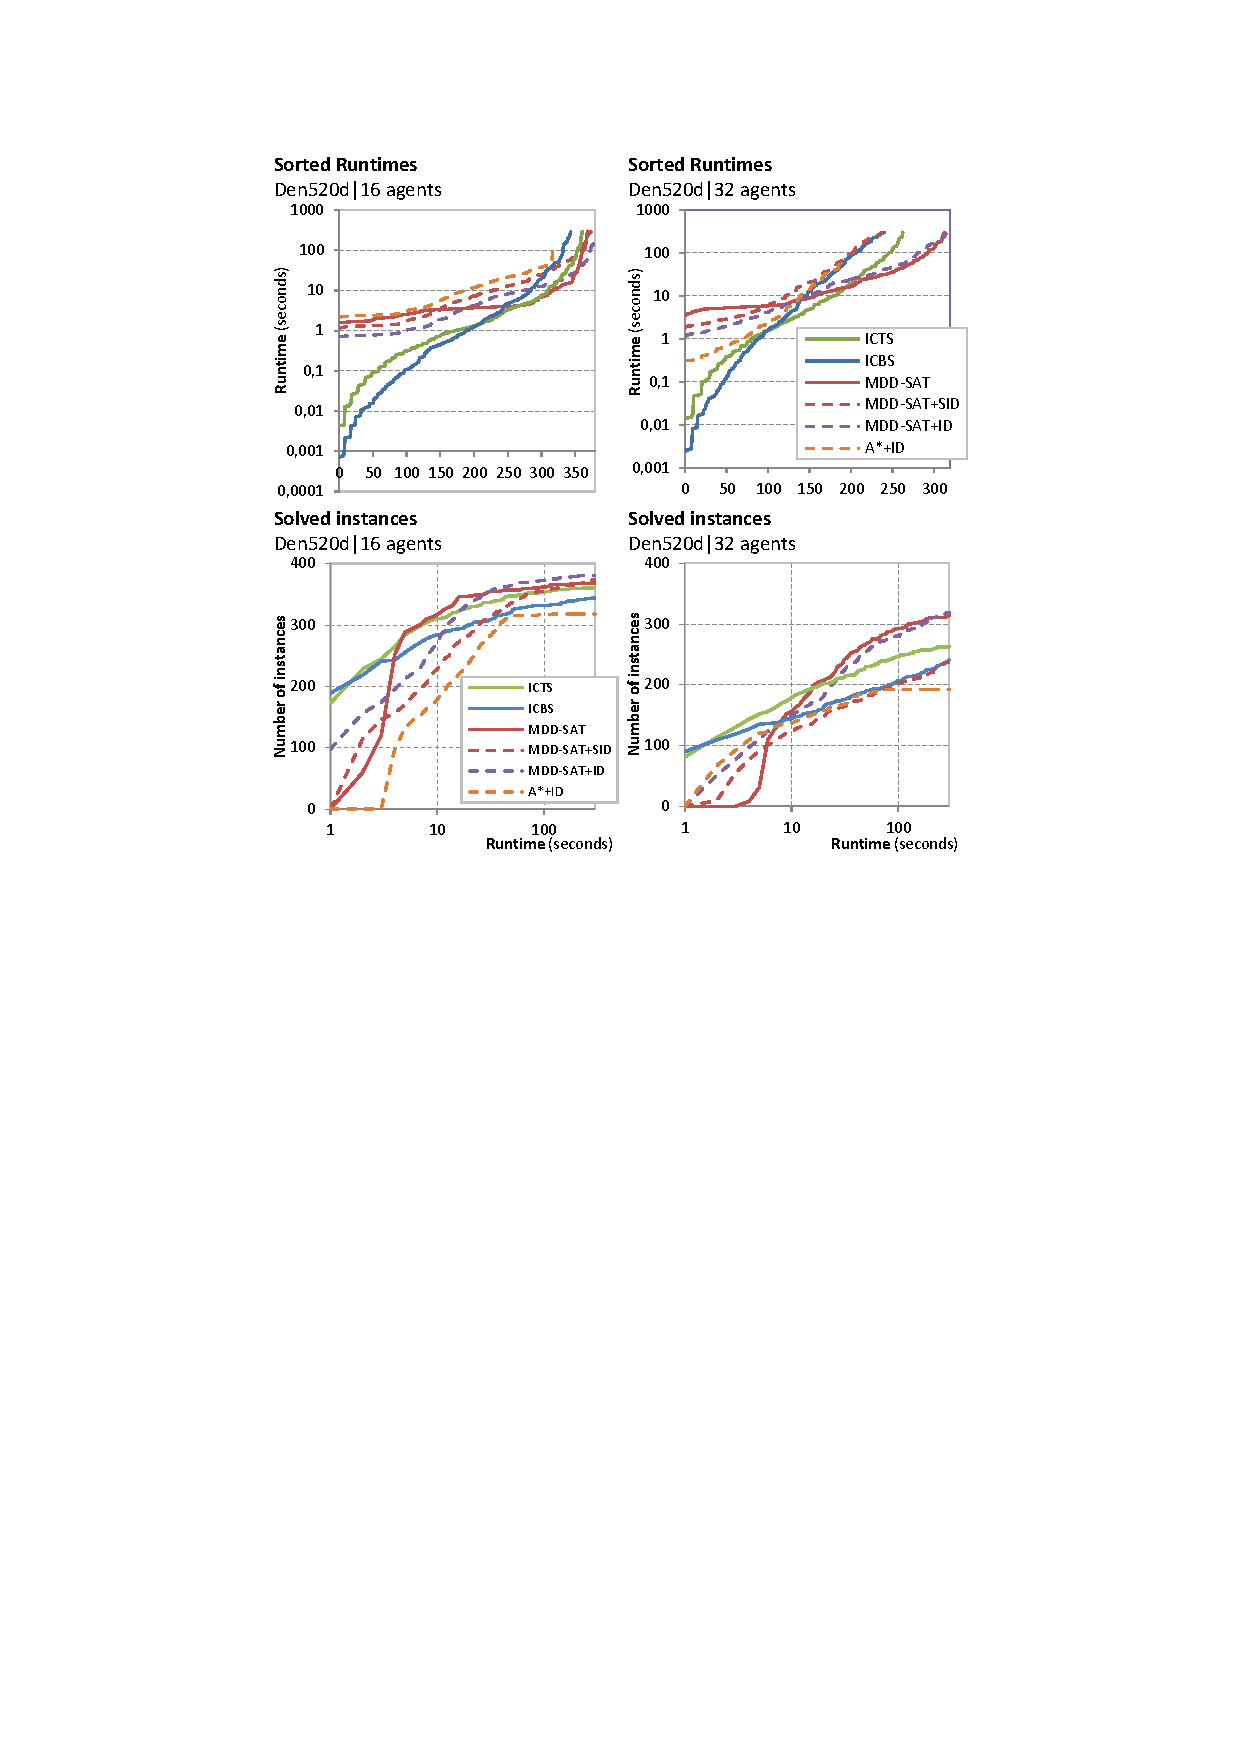
\includegraphics[trim={2.5cm 15.0cm 2.5cm 2.6cm},clip,width=1.0\textwidth]{expr-id_den520_sorted.pdf}
\vspace{-0.6cm}\caption{Runtime results with ID and SID for \texttt{den520} DAO map. Sorted runtimes (top) and the number of solved instances as a function of time are shown (bottom).}
\label{figure-den520-sorted-id}
\end{figure}

\begin{figure}[h]
\centering
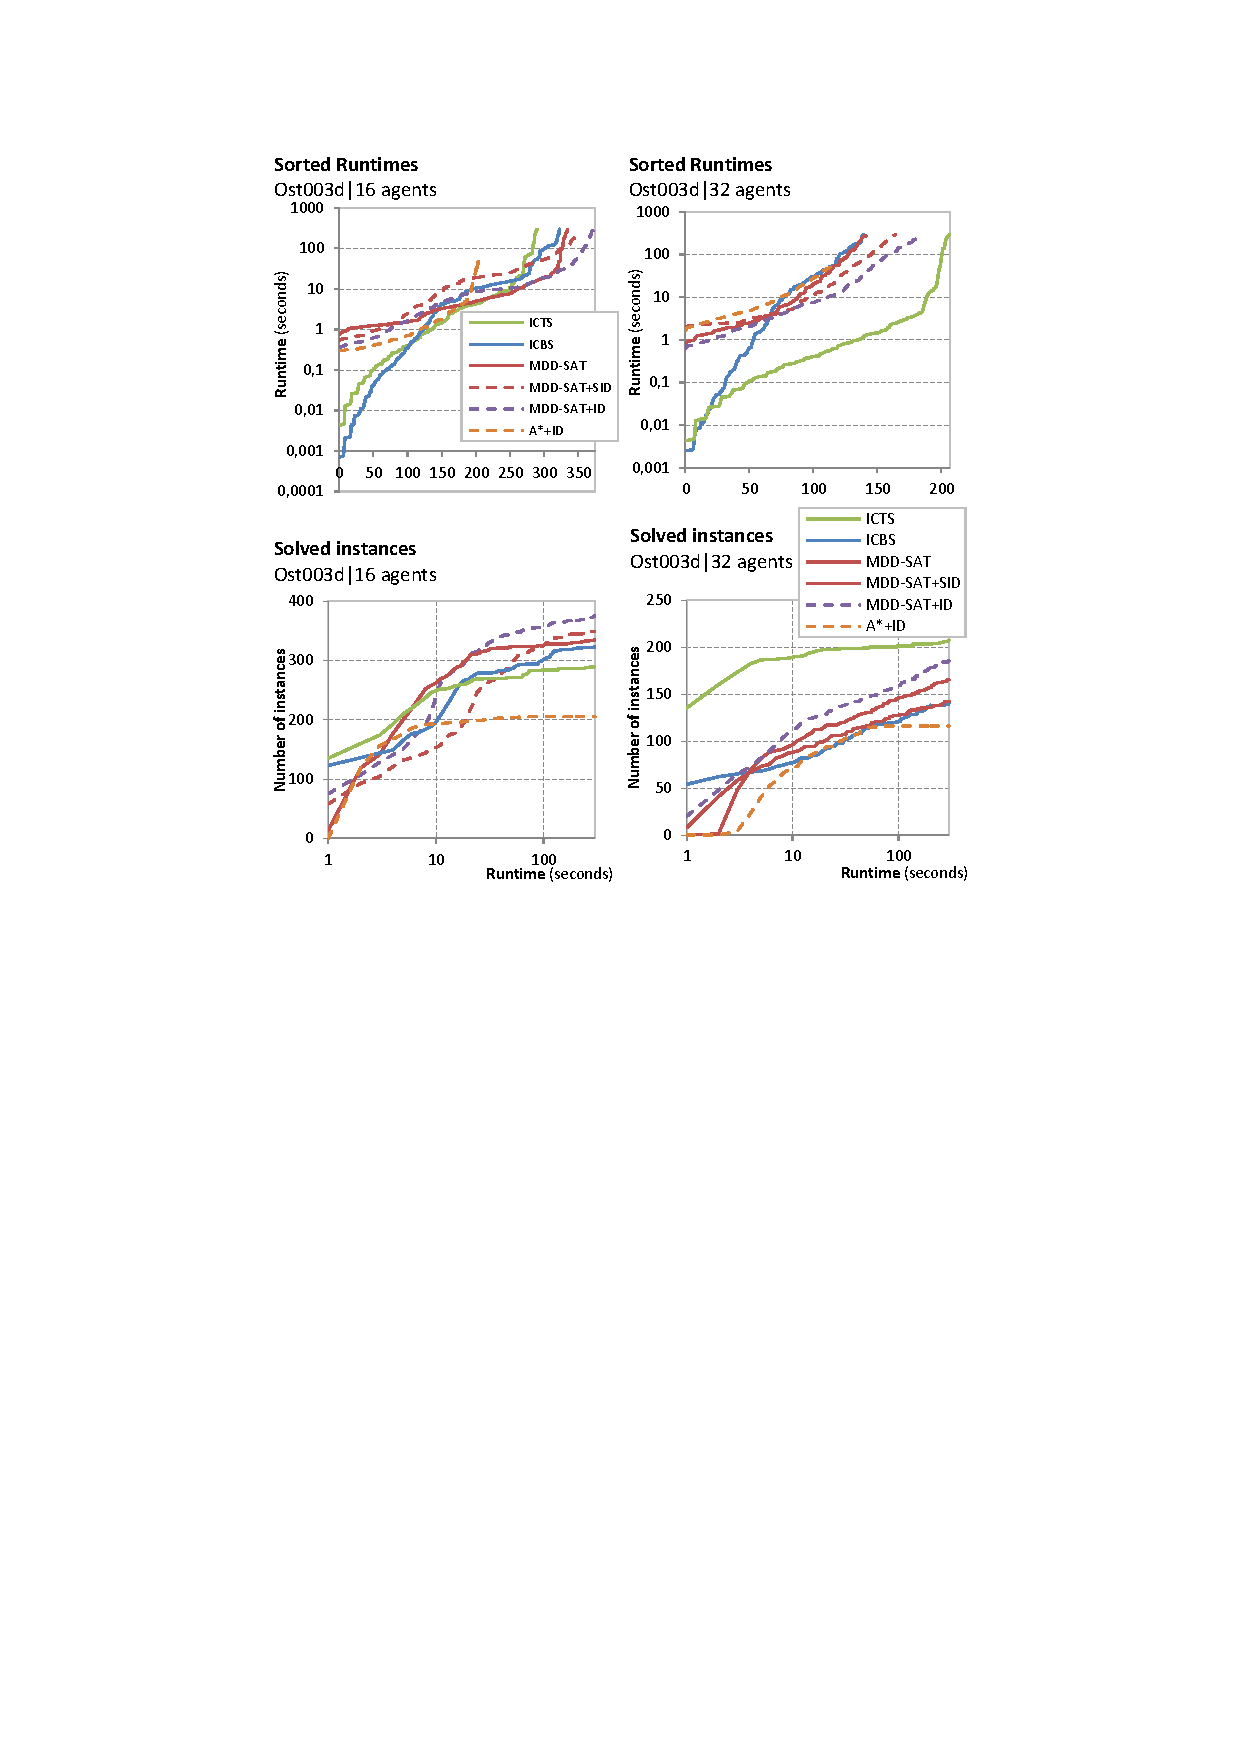
\includegraphics[trim={2.5cm 14.5cm 2.5cm 2.6cm},clip,width=1.0\textwidth]{expr-id_ost003_sorted.pdf}
\vspace{-0.6cm}\caption{Runtime results with ID and SID for \texttt{ost003} DAO map. Sorted runtimes (top) and the number of solved instances as a function of time are shown (bottom).}
\label{figure-ost003-sorted-id}
\end{figure}

\subsubsection{Results of Independent Detection on Large Maps}

Instances using DAO maps contained 16 and 32 agents. To obtain various difficulties we varied the distance of agents from their goals. This is again identical to the previous experimental setup with DAO maps. MDD-SAT with versions integrating SID and ID are compared. Results for DAO maps \texttt{brc202d}, \texttt{den520d}, and \texttt{ost003d} are shown in Figures \ref{figure-brc202-sorted-id}, \ref{figure-den520-sorted-id}, and \ref{figure-ost003-sorted-id}.

Results offers various patterns and it seems that no easy generalization valid across all types of maps is possible. Results suggest that structure of the map plays an important role.
On the \texttt{brc202d} map we can observe that SID leads to a better performance only in minority of cases of easy instances where the distance from the goal small. In all other cases, SID represents an overhead and the plain MDD-SAT performs better. ID on the other hand has some observable benefit, we can see that for hard instances with 32 agents MDD-SAT+ID performs as the best.

The explanation of this behavior rests in the structure of the map which consists of long narrow corridors. After having the goal positions far enough from the initial positions, agents inevitably interact through encountering each other in the corridors and are merged into larger groups which pushes the performance of both ID and SID towards and behind the plain MDD-SAT. However the overhead with independence detection has slower growth than the complexity of solving one large group of agents which explains the convergence the performance of MDD-SAT and the versions with SID and ID in harder instances and better performance of MDD-SAT+ID in case of 32 agents.

The \texttt{den520d} map features a different structure. It can be regarded as one large open space surrounded by a shaped border. Such structure suggests a hypothesis that when the distance from the goal is small then lot of independence could be detected and both SID and ID should improve the plain MDD-SAT. The verification against actual results supports the hypothesis. In addition to this, we can observe that longer distance from the goals causes worse performance of both SID and ID with respect to the plain MDD-SAT. Longer paths often go near the boundary of the open space where agents have an opportunity to meet each other and the group merging often arises from such situation.

The \texttt{ost003d} map can be regarded as relatively large open rooms separated by walls with narrows doors. This is again a different structure from both previous maps. Here we should expect that shortest paths need to touch the walls and corners which is again a situation that can give rise to the group merging. Comparing the shape of \texttt{den520d} and \texttt{ost003d} we can see that it is more likely to touch a wall or a corner in \texttt{ost003d} than touching the open space boundary in the \texttt{den520d} map. Results supports this hypothesis as we can see that significantly better performance is achieved with SID and ID only in a small portion of instances with the small distance from the goals. We can also observe that ID improves the plain MDD-SAT significantly in hard instances which suggests that we are able to detect non-trivial independences in such cases. Again the overhead caused by using ID is less time consuming than the extra time needed to solve one large group instead of several smaller groups.


\section{Bounded Suboptimal SAT-Based MAPF Solving}
\label{sec:suboptimal}

The versatility of SAT-based approach for solving MAPF can be further demonstrated by adapting it for suboptimal variants of the problem. Adaptation for suboptimal variants has been successfully done with search-based solvers including \textsc{Icts} \cite{DBLP:conf/socs/AljalaudS13} and \textsc{Cbs} \cite{DBLP:conf/ecai/BarerSSF14}. The motivation behind having a suboptimal solver is that we can trade-off the quality of solutions with respect to a given objective and the runtime. Usually lower quality solutions can be obtained faster \footnote{Ignoring the quality completely could open opportunity to use polynomial time algorithms like \textsc{Push-and-Rotate} \cite{DBLP:journals/jair/WildeMW14} or BIBOX \cite{DBLP:conf/icra/Surynek09} where runtime is usually not a problematic factor.}. In the bounded case, we have the control of how much do we tolerate the suboptimal solution to differ from the ideal optimal one.

In this section, we show how to convert MDD-SAT to a bounded suboptimal algorithm for the sum-of-costs objective. Converting MDD-SAT to a suboptimal any solution algorithm can be simply done by removing the cardinality constraints from the construction of $\mathcal{F}(\mu_0,\xi_0,\Delta)$. Let $\mathcal{F'}(\mu_0, \Delta)$ denote the resulting formula.  Since $\mathcal{F'}(\mu_0,\Delta)$ has all constraints from original $\mathcal{F}(\mu_0,\xi_0,\Delta)$ except the cardinality constraints, then clearly a satisfying assignment to $\mathcal{F'}(\mu_0, \Delta)$ still represents a feasible solution (no collisions between agents etc.). Since $\mathcal{F'}(\mu_0, \Delta)$ is less constrained than $\mathcal{F}(\mu_0,\xi_0, \Delta)$, we expect it to be solved faster. Indeed, we observed this in our preliminary experiments. Using $\mathcal{F'}(\mu_0, \Delta)$ in Algorithm~\ref{alg-MAPF-SAT-soc} instead of $\mathcal{F}(\mu_0,\xi_0, \Delta)$, however, looses the sum-of-cost optimality. 

Hence, replacing $\mathcal{F}(\mu_0,\xi_0, \Delta)$ with $\mathcal{F'}(\mu_0, \Delta)$ in Algorithm~\ref{alg-MAPF-SAT-soc} leads to a suboptimal version of the MDD-SAT solver that is faster than the optimal version. We refer to this unbounded version of MDD-SAT denoted as {\bf uMDD-SAT}.

A key question is what is the suboptimality of the solutions returned by uMDD-SAT? Is it really unbounded? We show later that even without the cardinality constraints, the suboptimality of the solutions outputted is bounded, due to how $\mathcal{F}(\mu_0,\xi_0, \Delta)$ and $\mathcal{F'}(\mu_0, \Delta)$ are constructed. 

Next, we show how to control the suboptimality of the returned solution by introducing a relaxed version of the optimal cardinality constraints, allowing the algorithm's user to balance the runtime and the suboptimality.


\subsection{Bounded Suboptimal Version of MDD-SAT}

% The key to our bounded-suboptimal SAT-based solver is that it modified the $\Delta$ parameter used in construction of $\mathcal{F}(\mu_0,\xi_0, \Delta)$. In MDD-SAT, $\Delta$ is incremented by one in every iteration. Allowing $\Delta$ parameter to be less restrictive; that is, replace $\Delta$ with $\Delta'=\Delta+\delta$, where $\delta \geq 0$ is an integer value, produces formula of the same size but representing more  solutions. \footnote{The change from $\Delta$ to $\Delta'$ does not affect the number of clauses that represent the cardinality constraint, because we encoded the cardinality constraints using a sequential counter, whose size is proportional to the number of propositional variable involved but not to the value of the bound \cite{DBLP:conf/cp/Sinz05}.} Since $\Delta'>\Delta$, we expect a formula with the sum-of-costs bounded by $\Delta'$ to be easier to solve than that with the original $\Delta$.

The key to our bounded-suboptimal SAT-based solver is that it splits the $\Delta$ parameter used in construction of $\mathcal{F}(\mu_0,\xi_0, \Delta)$ into two parameters $\Delta_\mu$ and $\Delta_\xi$. 
The resulting formulae, denoted $\mathcal{F}(\mu_0,\xi_0, \Delta_\mu, \Delta_\xi)$, represents the decision problem ``is there a valid solution to the given MAPF problem with a makespan smaller than or equal to $\mu_0+\Delta_\mu$ and a sum-of-costs smaller than or equal to $\xi_0+\Delta_\xi$''.
 
One can view MDD-SAT as solving a sequence of such decision problem, setting $\Delta_\mu=\Delta_\xi=\Delta$ and incrementing both $\Delta_\mu$ and $\Delta_\xi$ by one in every iteration.  To return bounded-suboptimal solutions, we allow $\Delta_\xi$ to be less restrictive; that is, larger than $\Delta_\mu$ by some integer value $\delta\geq 0$. 
This produces a formula  $\mathcal{F}(\mu_0,\xi_0, \Delta, \Delta+\delta)$ which is approximately the same size as $\mathcal{F}(\mu_0,\xi_0, \Delta)$ but represents more solutions\footnote{The MDDs used for construction of $\mathcal{F}(\mu_0,\xi_0, \Delta, \Delta+\delta)$ are identical as those for $\mathcal{F}(\mu_0,\xi_0, \Delta)$ but the former uses different cost bounds in the cardinality constraints whose encoding based on sequential counter has the size proportional to the value of the bound \cite{DBLP:conf/cp/Sinz05}.}. Since $\Delta+\delta>\Delta$, we expect a formula with the sum-of-costs bounded by $\Delta+\delta$ to be easier to solve than that with the original $\Delta$.

%\footnote{The change $\Delta_\xi$ from $\Delta$ to $\Delta+\delta$ does not affect the number of clauses that represent the cardinality constraint, because we encoded the cardinality constraints using a sequential counter, whose size is proportional to the number of propositional variable involved but not to the value of the bound \cite{DBLP:conf/cp/Sinz05}.}

The following proposition shows that for a solvable MAPF $\Sigma$ the sum-of-costs of the solution obtained by the above process differs from the optimal one by at most $\delta$.

\begin{proposition}
Let $\delta$ be a non-negative integer and let $\mathcal{F}(\mu_0, \xi_0, \Delta, \Delta+\delta)$ be the first satisfiable formula found in the sequence of formulae $\mathcal{F}(\mu_0, \xi_0, 0, \delta)$, $\mathcal{F}(\mu_0, \xi_0, 1, 1+\delta)$,...,$\mathcal{F}(\mu_0, \xi_0, \Delta-1, \Delta+\delta-1)$, $\mathcal{F}(\mu_0+\Delta, \xi_0, \Delta, \Delta+\delta)$. Then the solution represented by $\mathcal{F}(\mu_0, \xi_0, \Delta,\Delta+\delta)$ has sum-of-costs $\xi \leq \xi_{opt} + \delta$ where $\xi_{opt}$ is the optimal sum-of-costs for input MAPF $\Sigma$.
\label{prop:bound}
\end{proposition}

\noindent {\bf Proof:} Since $\mathcal{F}(\mu_0, \xi_0, \Delta,\Delta+\delta)$ is the first satisfiable formula in the sequence, we know that previous formula $\mathcal{F}(\mu_0,\xi_0,\Delta-1,\Delta+\delta-1)$ is not solvable. This means that no solution of makespan at most $\mu_0+\Delta-1$ and sum-of-costs at most $\xi_0+\Delta+\delta - 1$ exists. In addition to this, we know that all solutions of sum-of-costs $\xi_0+\Delta-1$ fit under the makespan of at most $\mu_0+\Delta-1$.

Hence unsolvability of $\mathcal{F}(\mu_0, \xi_0,\Delta-1,\Delta+\delta-1)$ together with $\delta \geq 0$ implies that there is no solution of sum-of-costs smaller than or equal to $\xi_0+\Delta-1$ (without restricting the makespan) since otherwise $\mathcal{F}(\mu_0, \xi_0, \Delta-1,\Delta+\delta-1)$ would be solvable. Therefore, the optimal sum-of-costs is at least $\xi_0+\Delta$. The solvability of $\mathcal{F}(\mu_0, \xi_0,\Delta,\Delta+\delta)$ tells that there is a solution of $\Sigma$ of sum-of-costs $\xi_0+\Delta+\delta$ which differs from the optimum by at most $\delta$. $_\blacksquare$\\

Observe that the only property of $\delta$ we used was that it is a non-negative integer but there is no requirement that it must be constant across individual iterations of the algorithm. Proposition~\ref{prop:bound} holds even if we use a non-negative $\delta$ as a function of $\Delta$ instead of a constant. This property can be used to modify the above SAT-based framework to a $(1+\epsilon)$-bounded suboptimal algorithm. That is, the algorithm produces solutions that are no worse than $(1+\epsilon)$ times than the optimum. How to calculate $\delta$ from given $\epsilon$ is summarized in the following corollary.

\begin{corollary}
Given an error $\epsilon>0$ the iterative SAT-based suboptimal framework can modified to an $(1+\epsilon)$-bounded suboptimal algorithm by appropriate setting of $\delta$.
\end{corollary}

\noindent {\bf Proof:} As $\delta$ is in fact a function of the number of iterations we will use notation $\delta(\Delta)$. Let $\delta(\Delta)=\epsilon \cdot (\xi_0+\Delta)$. Then the sum-of-costs of the solution returned by the algorithm is at most $(1+\epsilon) \cdot (\xi_0+\Delta)$. Following the arguments from the proof of Proposition \ref{prop:bound}, the optimal sum-of-costs is at least $\xi_0+\Delta$ hence the ratio between the sum-of-costs of returned solution and the optimum is at most $(1+\epsilon)$. $_\blacksquare$\\

The pseudo-code of the $(1+\epsilon)$-bounded suboptimal version of the MDD-SAT algorithm is
presented as Algorithm \ref{alg-eMDD-SAT}. We refer to this algorithm as {\bf eMDD-SAT}.


%\begin{definition}
%\textit{Time expansion graph}  of depth $\mu$ is a digraph $(V,E)$ where
%$V=\{u^t_j|t=0,1,...,\mu \wedge u_j \in V\}$ and $E \subseteq \{
%{(u_j^t,u_k^{t+1})} | t=0,1,...,\mu-1\ \wedge (\{u_j,u_k\} \in E
%\vee j=k) \}$. \label{def:modifiedExpansionGraph}
%\end{definition}

\begin{algorithm}[t]
\begin{footnotesize}
\SetAlgoLined \SetKwBlock{NRICL}{eSolve-MDD-SAT$_{SOC}$(MAPF
$\Sigma=(G=(V,E),A,\alpha_0,\alpha_+)$,$\epsilon$)}{end} \NRICL{
   \If {$\Sigma$ is unsolvable}{
     \Return $\mathit{UNSOLVABLE}$\\
   } 
   $\mu_0=\max_{a_i\in A} \xi_0(a_i)$\\
   $\xi_0 = \sum_{a_i\in A} \xi_0(a_i)$ \\
   $\Delta \gets 0$\\
   \While {$\mathit{TRUE}$} {
         $\Delta_\mu \gets \Delta$\\
         $\delta \gets \epsilon \cdot (\xi_0 +\Delta)$ \\         
         $\Delta_\xi \gets \Delta_\mu + \delta$ \\
         
         $\mathcal{F}(\mu_0, \xi_0, \Delta_\mu, \Delta_\xi) \gets$ encode-MAPF($\Sigma$, $\mu_0$, $\xi_0$, $\Delta_\mu$, $\Delta_\xi$)\\
         $\pi \gets$ consult-SAT-SOLVER($\mathcal{F}(\mu_0, \xi_0, \Delta_\mu, \Delta_\xi)$)\\
         \If {$\pi \neq \mathit{UNSAT}$}{
        	\Return $\pi$\\
        }
        $\Delta \gets \Delta + 1$\\         
    }
} \caption{eMDD-SAT, an $(1+\epsilon)$-bounded suboptimal version of the MDD-SAT MAPF solver} \label{alg-eMDD-SAT}
\end{footnotesize}
\end{algorithm}

Let us note that a further minor improvement of the pseudo-code could be done which uses a basic relation of time expansion used in the formula. Observe that in any solution to an MAPF problem it holds that $\mu \leq \xi \leq {k\cdot\mu}$ where $k$ is the number of agents. Therefore, if $\xi_0+\Delta+\delta(\Delta) \geq \mu \cdot k$, then there is no need to add any cardinality constraints to $\mathcal{F}(\mu,\Delta)$ to bound the sum-of-costs, since any solution of the makespan at most $\mu$ has automatically bounded its sum-of-costs by $\mu \cdot k$. 

This inequality represents a limit of the relaxation achievable by allowing more freedom over the cost bound imposed by the cardinality constraints. Hence the $(1+\epsilon)$-bounded suboptimal MDD-SAT algorithm tends to be near optimal anyway. The algorithm can be at most $\big(\frac{k \cdot (\mu_0 + \Delta)}{\xi_0+\Delta}\big)$-bounded.

\subsection{Experimental Results for uMDD-SAT and eMDD-SAT}

We again evaluated suboptimal variants of MDD-SAT on small grids with obstacles and on large DAO maps. The set of instances for small grids was the same as in the previous experiments. Again we changed number of agents from 1 until we reach unsolvable instances under the given runtime of 300 seconds. For each number of agents 10 instances with random initial and goal configuration were generated.

In DAO maps we varied the number of agents instead of varying the distance from their goals to obtain instances of various difficulties. The number of agents is varied from 1 to 256 where the steps is initially 1 and then increased to 16. Ten instances with random initial and goal configuration per number of agents were used.

\subsubsection{The Unbounded Variant: uMDD-SAT}

Comparison of unbounded algorithms including SAT-based \textsc{UniAGENT} \cite{DBLP:conf/ijcai/Surynek15}, \textsc{eCbs} \cite{DBLP:conf/ecai/BarerSSF14}, \textsc{Push-and-Swap} \cite{DBLP:conf/aaai/LunaB11}, and uMDD-SAT are shown in Figures \ref{expr-sub_grids-U-time-sorted}, \ref{expr-sub_grids-U-soc-sorted}, \ref{expr-sub_maps-U-sorted}, and \ref{expr-sub_maps-U-soc-sorted}.

All these algorithms represent different approaches to finding unbounded suboptimal solutions. \textsc{UniAGENT} is an unbounded suboptimal SAT-based method. Unlike MDD-SAT, the time expansion in the \textsc{UniAGENT} algorithm adds a new layer, a copy of the underlaying graph $G$, only after agents cannot avoid each other within the existing layers. \textsc{eCbs} is a representative of suboptimal search-based algorithms, a relaxation of CBS. \textsc{Push-and-Swap} on the other hand views the MAPF problem via transforming permutations of agents in the graph and is a major representative of rule-based algorithms.

Sorted runtimes of instances on $8{}\times{}8$, $16{}\times{}16$, and $32{}\times{}32$ grids solvable under the time limit are shown in Figure \ref{expr-sub_grids-U-time-sorted} (the lower line means faster algorithm). We can see clear dominance of the rule-based polynomial time \textsc{Push-and-Swap} algorithm whose runtime grows only moderately in more difficult instances. The opposite can be seen for search-based and compilation-based algorithms. Their runtime grows fast and in some cases \textsc{UniAgent} and uMDD-SAT fail to solve all instances. The \textsc{UniAgent} algorithm performs well only in harder instances on the $8{}\times{}8$ grid where it outperforms uMDD-SAT and is close to \textsc{eCbs}, but in other cases it is clearly loosing. Comparison of \textsc{eCbs} and uMDD-SAT does not show a clear winner. On easier instances \textsc{eCbs} tends to be faster white in harder cases uMDD-SAT tends to be faster.

\begin{figure}[h]
\centering
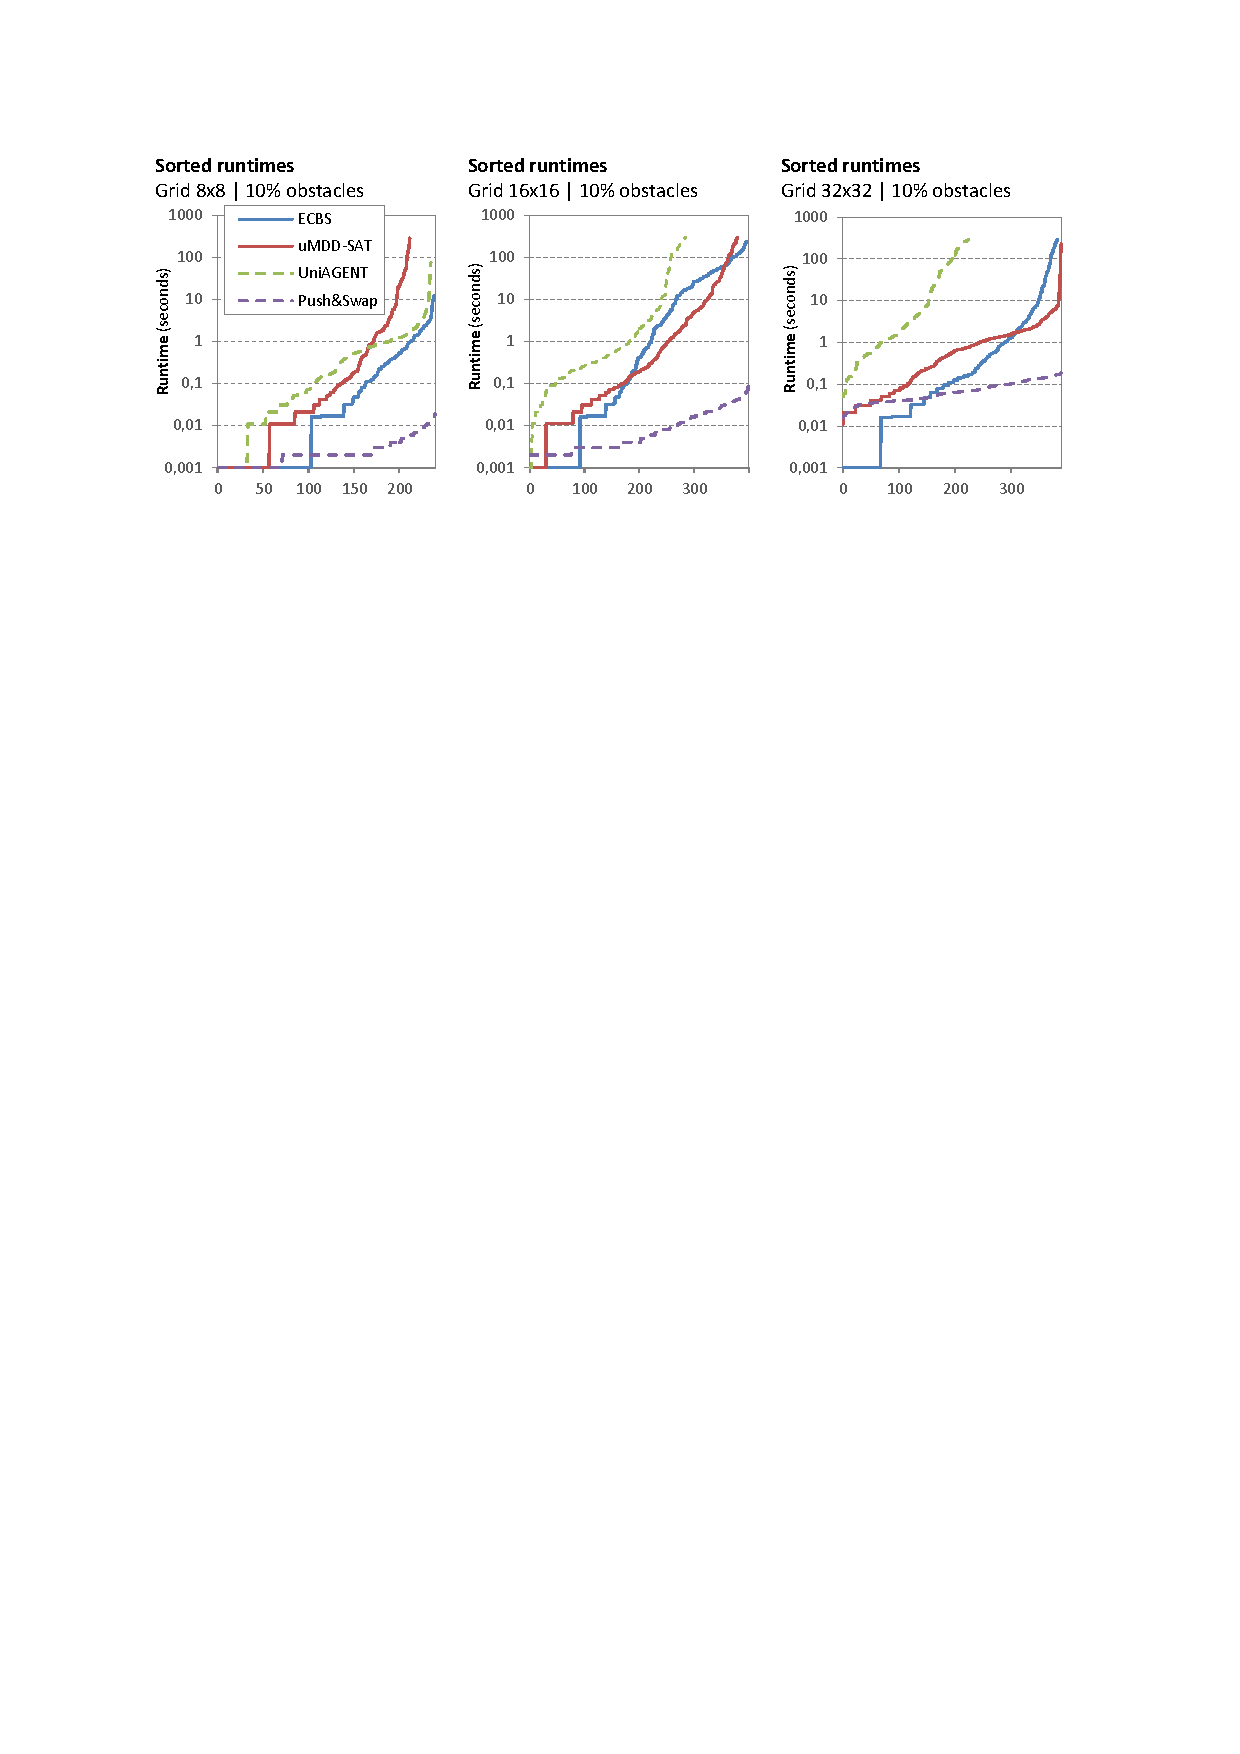
\includegraphics[trim={2.5cm 21.0cm 2.5cm 2.5cm},clip,width=\textwidth]{expr-sub_grids-U-sorted.pdf}
\vspace{-0.8cm}
\caption{Comparison of unbounded suboptimal solvers  - sorted runtimes for uMDD-SAT, \textsc{Push-and-Swap},  \textsc{eCbs}, and \textsc{UniAgent} are compared in $8{}\times{}8$, $16{}\times{}16$, and $32{}\times{}32$ grids.}
\label{expr-sub_grids-U-time-sorted}
\end{figure}

% Add optimal variant to plots, so that the difference from the optimum is visible.
% Improve description of sorting in plots.

To understand the performance of individual algorithms better we also present comparison of the sum-of-costs of solutions produced by tested algorithms in Figure \ref{expr-sub_grids-U-soc-sorted} (lower line is closer to the optimum). We can see here that although \textsc{Push-and-Swap} is the fastest algorithm the quality of its solutions it the worst, that is the sum-of-costs is the highest among all tested algorithms. Sum-of-costs in \textsc{UniAGENT} is also high. Comparison between uMDD-SAT and \textsc{eCbs} indicates that \textsc{eCbs} tends to generate lower sum-of-costs.

\begin{figure}[h]
\centering
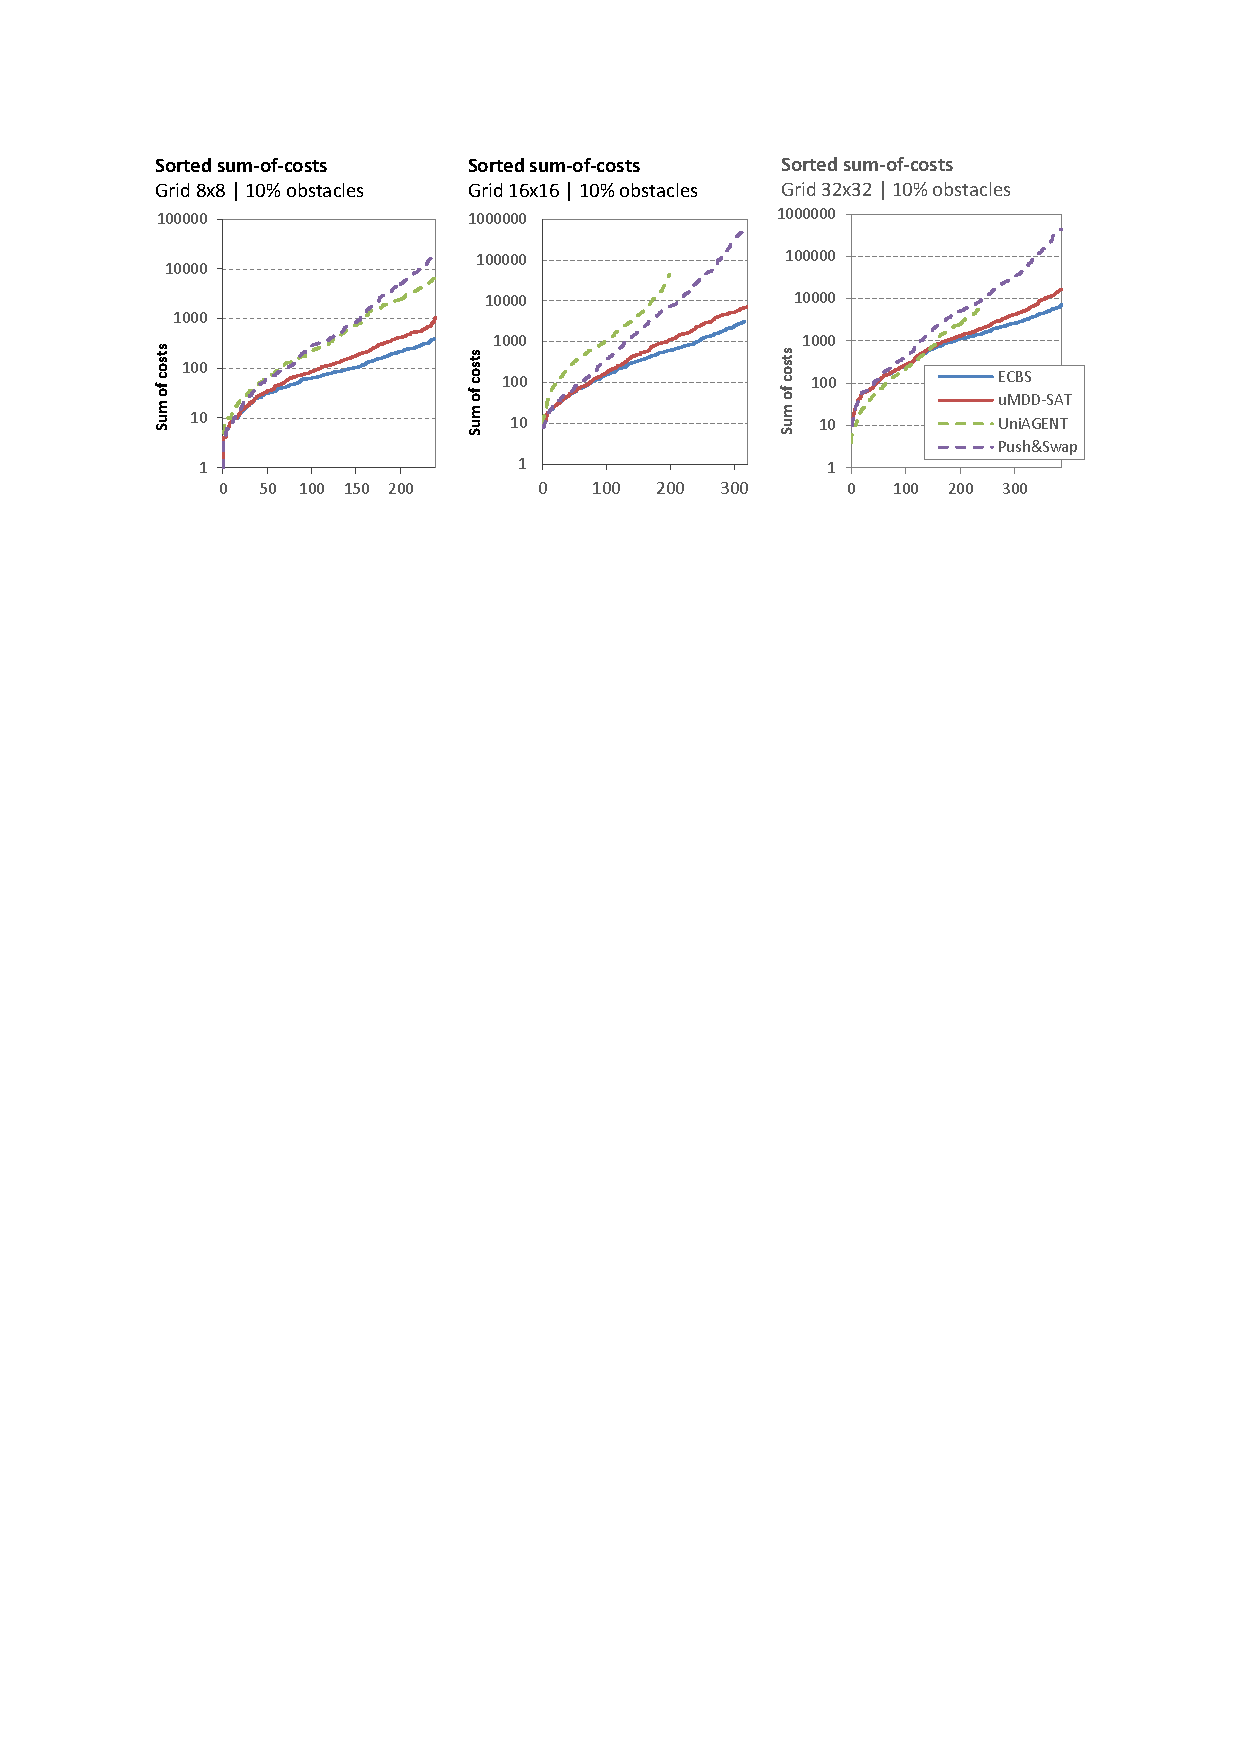
\includegraphics[trim={2.5cm 21.0cm 2.5cm 2.6cm},clip,width=\textwidth]{expr-sub_grids-soc-sorted.pdf}
\vspace{-0.8cm}
\caption{Comparison of solutions produced by unbounded suboptimal solvers  - sorted sum-of-costs of solutions by uMDD-SAT, \textsc{Push-and-Swap}, \textsc{eCbs}, and \textsc{UniAgent} are compared in $8{}\times{}8$, $16{}\times{}16$, and $32{}\times{}32$ grids.}
\label{expr-sub_grids-U-soc-sorted}
\end{figure}

The generalization from the observed trends is that even if we completely relax from the quality of solutions in search-based and compilation-based algorithms still their performance cannot match the polynomial-time rule-based methods. Another generalization is that despite the relaxation of the cost bound search-based and compilation-based algorithms tend to produce solutions of higher quality than rule-based algorithm does.

The explanation of the observed trends is that search-based and compilation-based algorithms eventually traverse search space of exponential size. Relatively good performance of \textsc{eCbs} can attributed to its greedy nature after the cost bound is relaxed which more likely leads to guessing a solution. On the other hand uMDD-SAT is slowed down by proving non-existence of solutions for lower makespans.

%\begin{figure}[h]
%\centering
%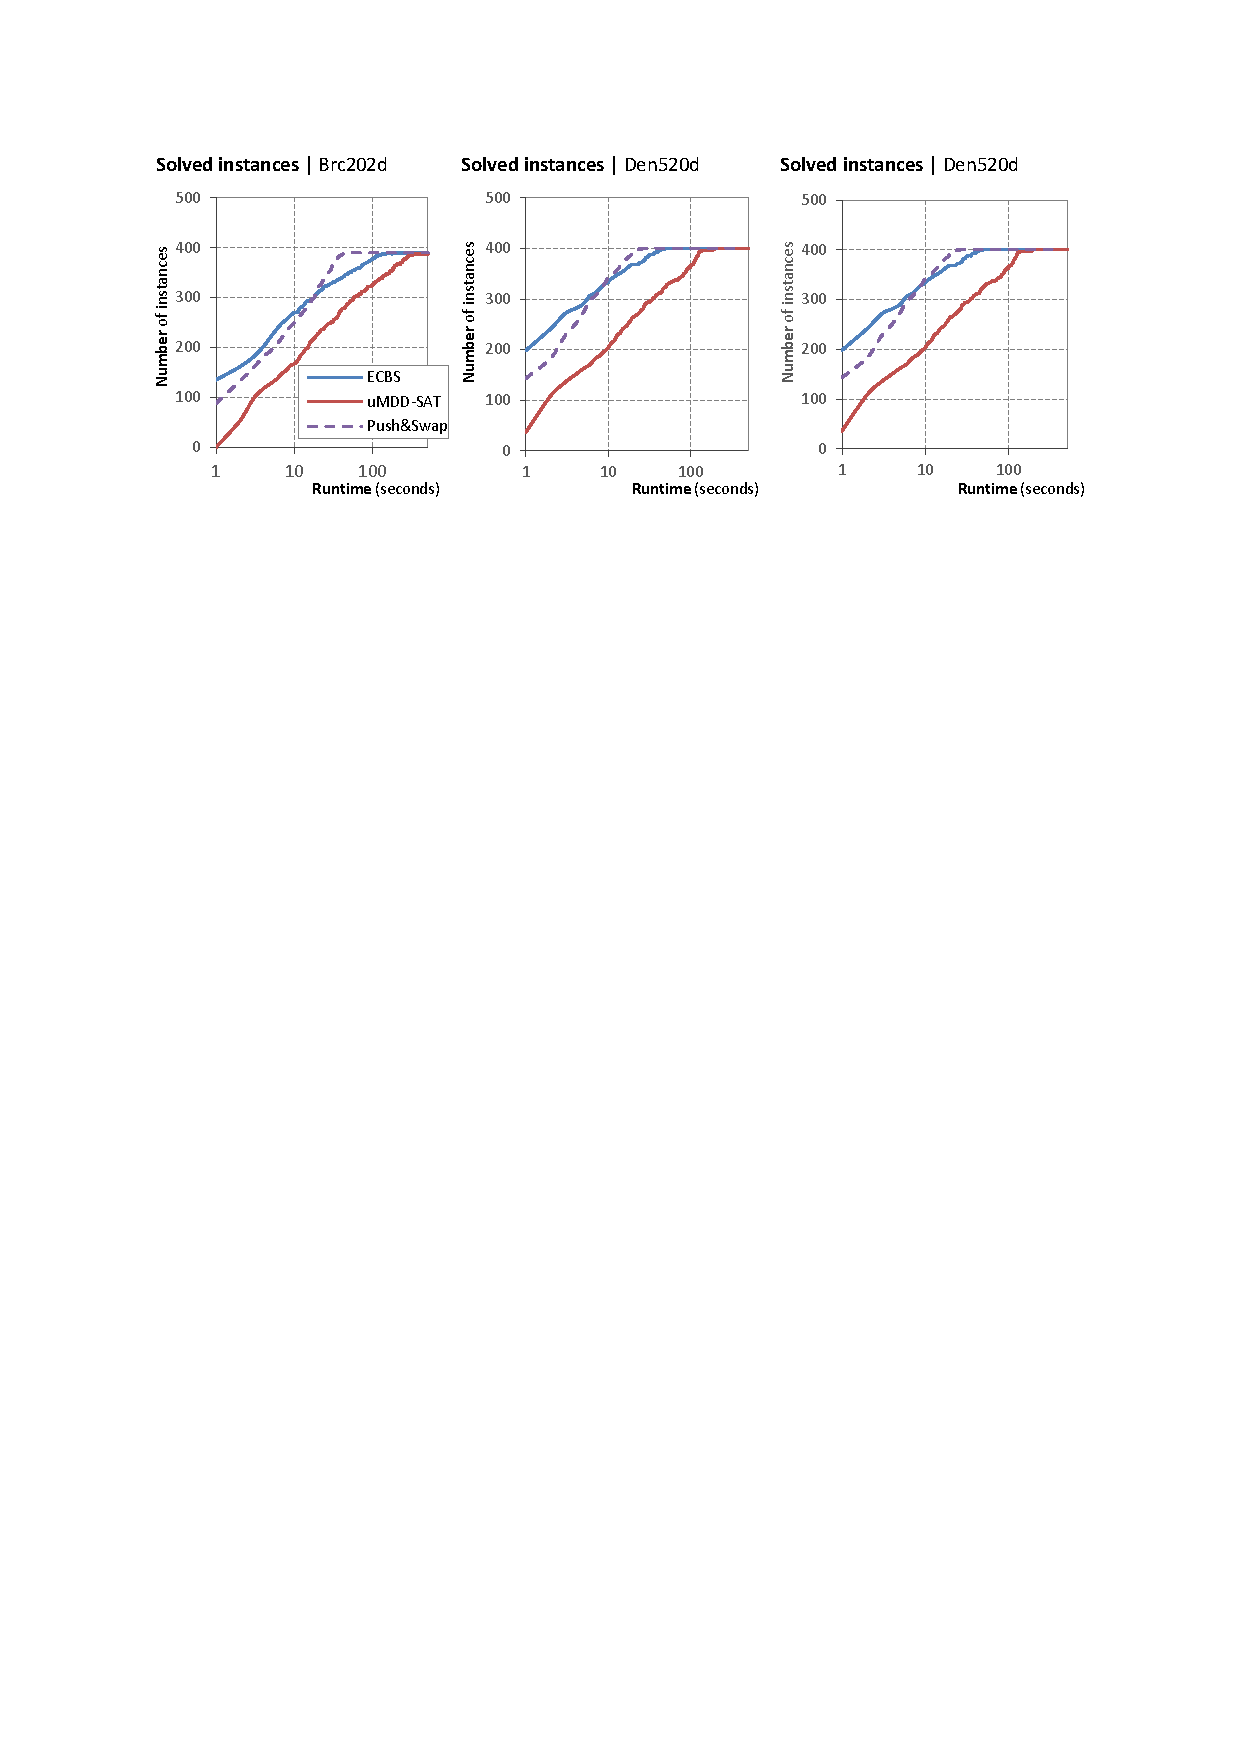
\includegraphics[trim={2.5cm 21.0cm 2.5cm 2.5cm},clip,width=\textwidth]{expr-sub_maps-U-num-solved.pdf}
%\vspace{-0.8cm}
%\caption{Comparison of unbounded suboptimal solvers on DAO maps - number of solvable instances for uMDD-SAT, \textsc{eCbs}, and \textsc{Push-and-Swap} as a function of runtime (the horizontal runtime axis uses logarithmic scale).}
%\label{expr-sub_maps-U-num-solved}
%\end{figure}

Results of the test of unbounded algorithms on large DAO maps is reported in Figures \ref{expr-sub_maps-U-sorted} and  \ref{expr-sub_maps-U-soc-sorted}. The former shows sorted runtimes while the latter shows sorted sum-of-costs (lower plot means a better results in both figures). Due to its weak performance on large maps, the \textsc{UniAGENT} algorithm was omitted in this test.

\begin{figure}[h]
\centering
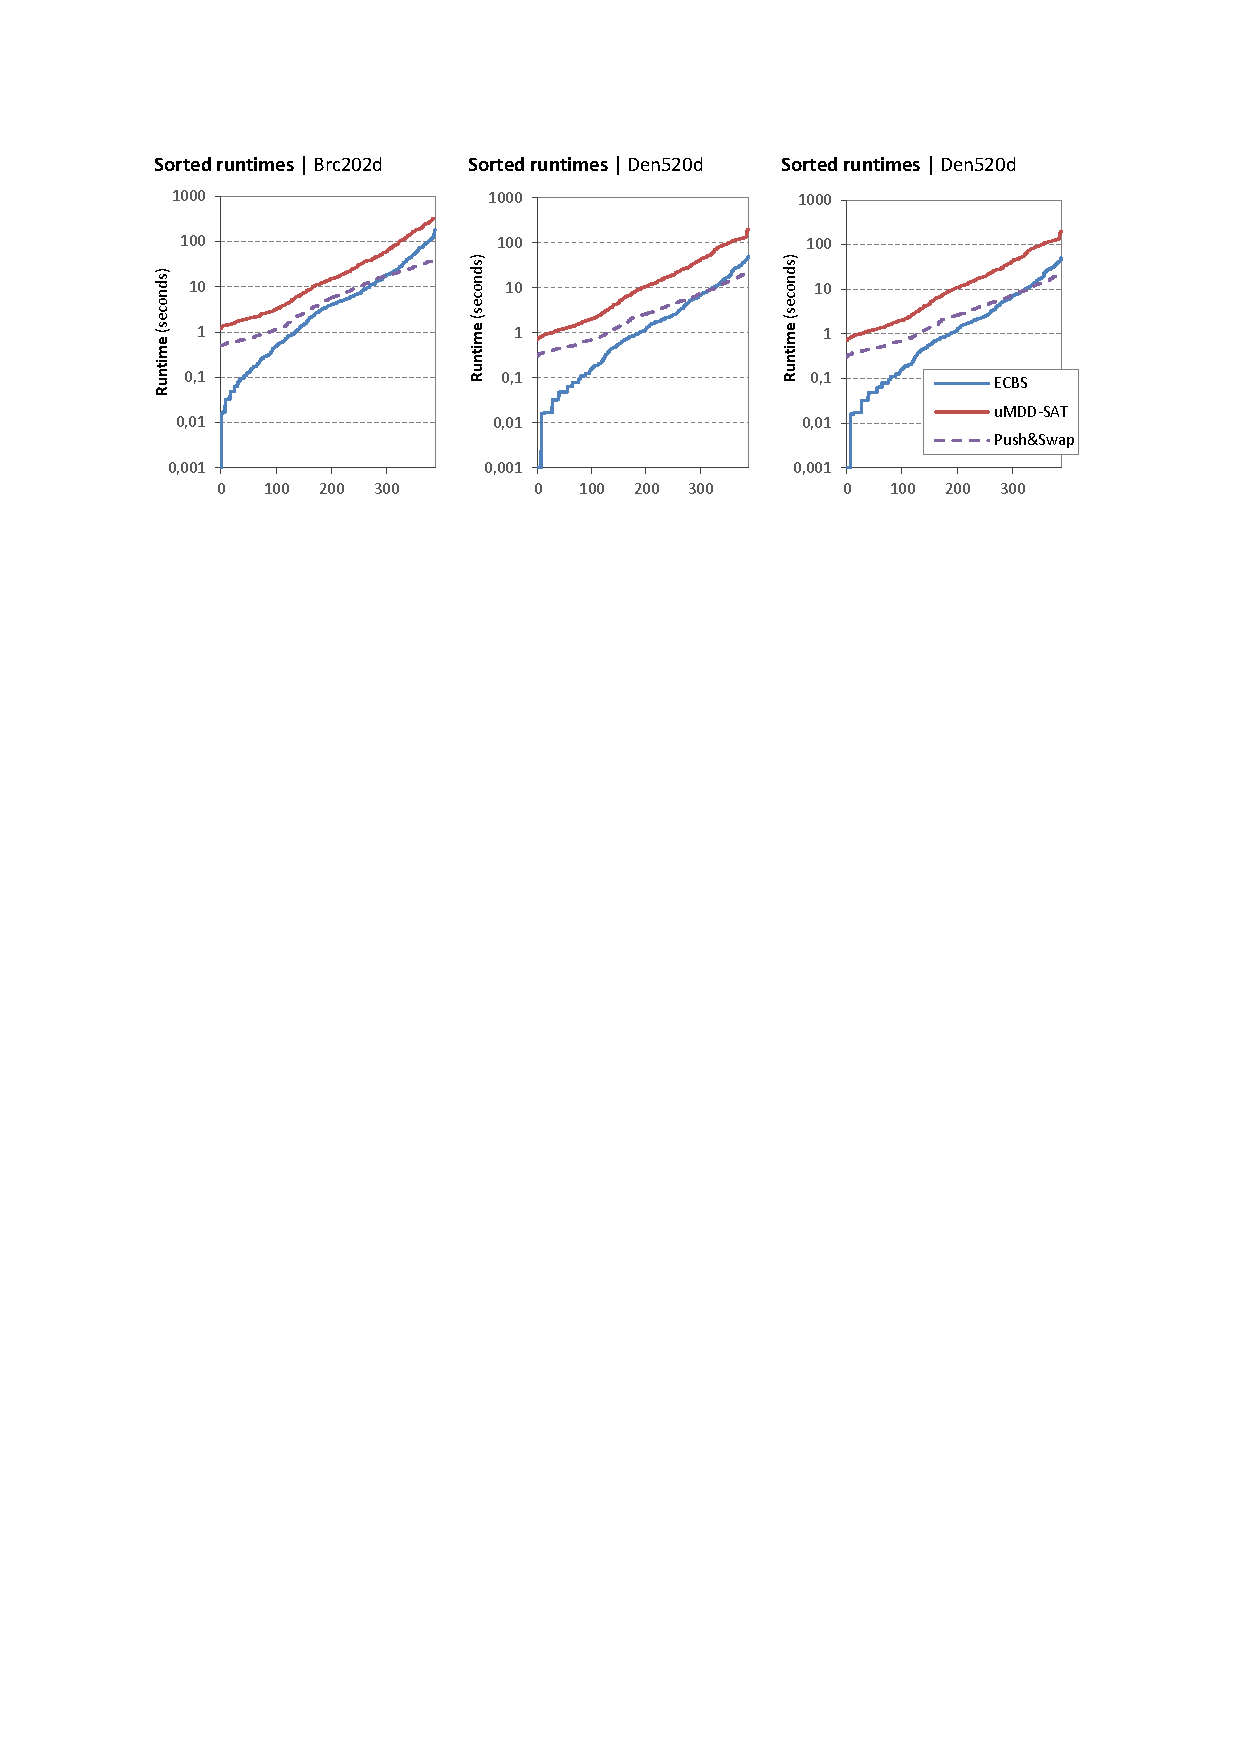
\includegraphics[trim={2.5cm 21.0cm 2.5cm 2.5cm},clip,width=\textwidth]{expr-sub_maps-U-sorted.pdf}
\vspace{-0.8cm}
\caption{Comparison of unbounded suboptimal solvers on DAO maps - sorted runtimes for uMDD-SAT, \textsc{eCbs}, and \textsc{Push-and-Swap}.}
\label{expr-sub_maps-U-sorted}
\end{figure}

Results indicate clear dominance of the \textsc{eCbs} algorithm which consistently outperforms the uMDD-SAT algorithm and even \textsc{Push-and-Swap} except hardest cases containing many agents. There is no significant difference in the sum-of-costs of solutions of uMDD-SAT and \textsc{eCbs} but  \textsc{Push-and-Swap} produces solutions with significantly higher sum-of-costs. These trends can be explained two-fold: (i) uMDD-SAT has relatively big overhead of constructing large MDDs and it must often prove the non-existence of a solution which is hard; (ii) \textsc{eCbs} has a great freedom to navigate itself greedily towards guessing a correct solution.

\begin{figure}[h]
\centering
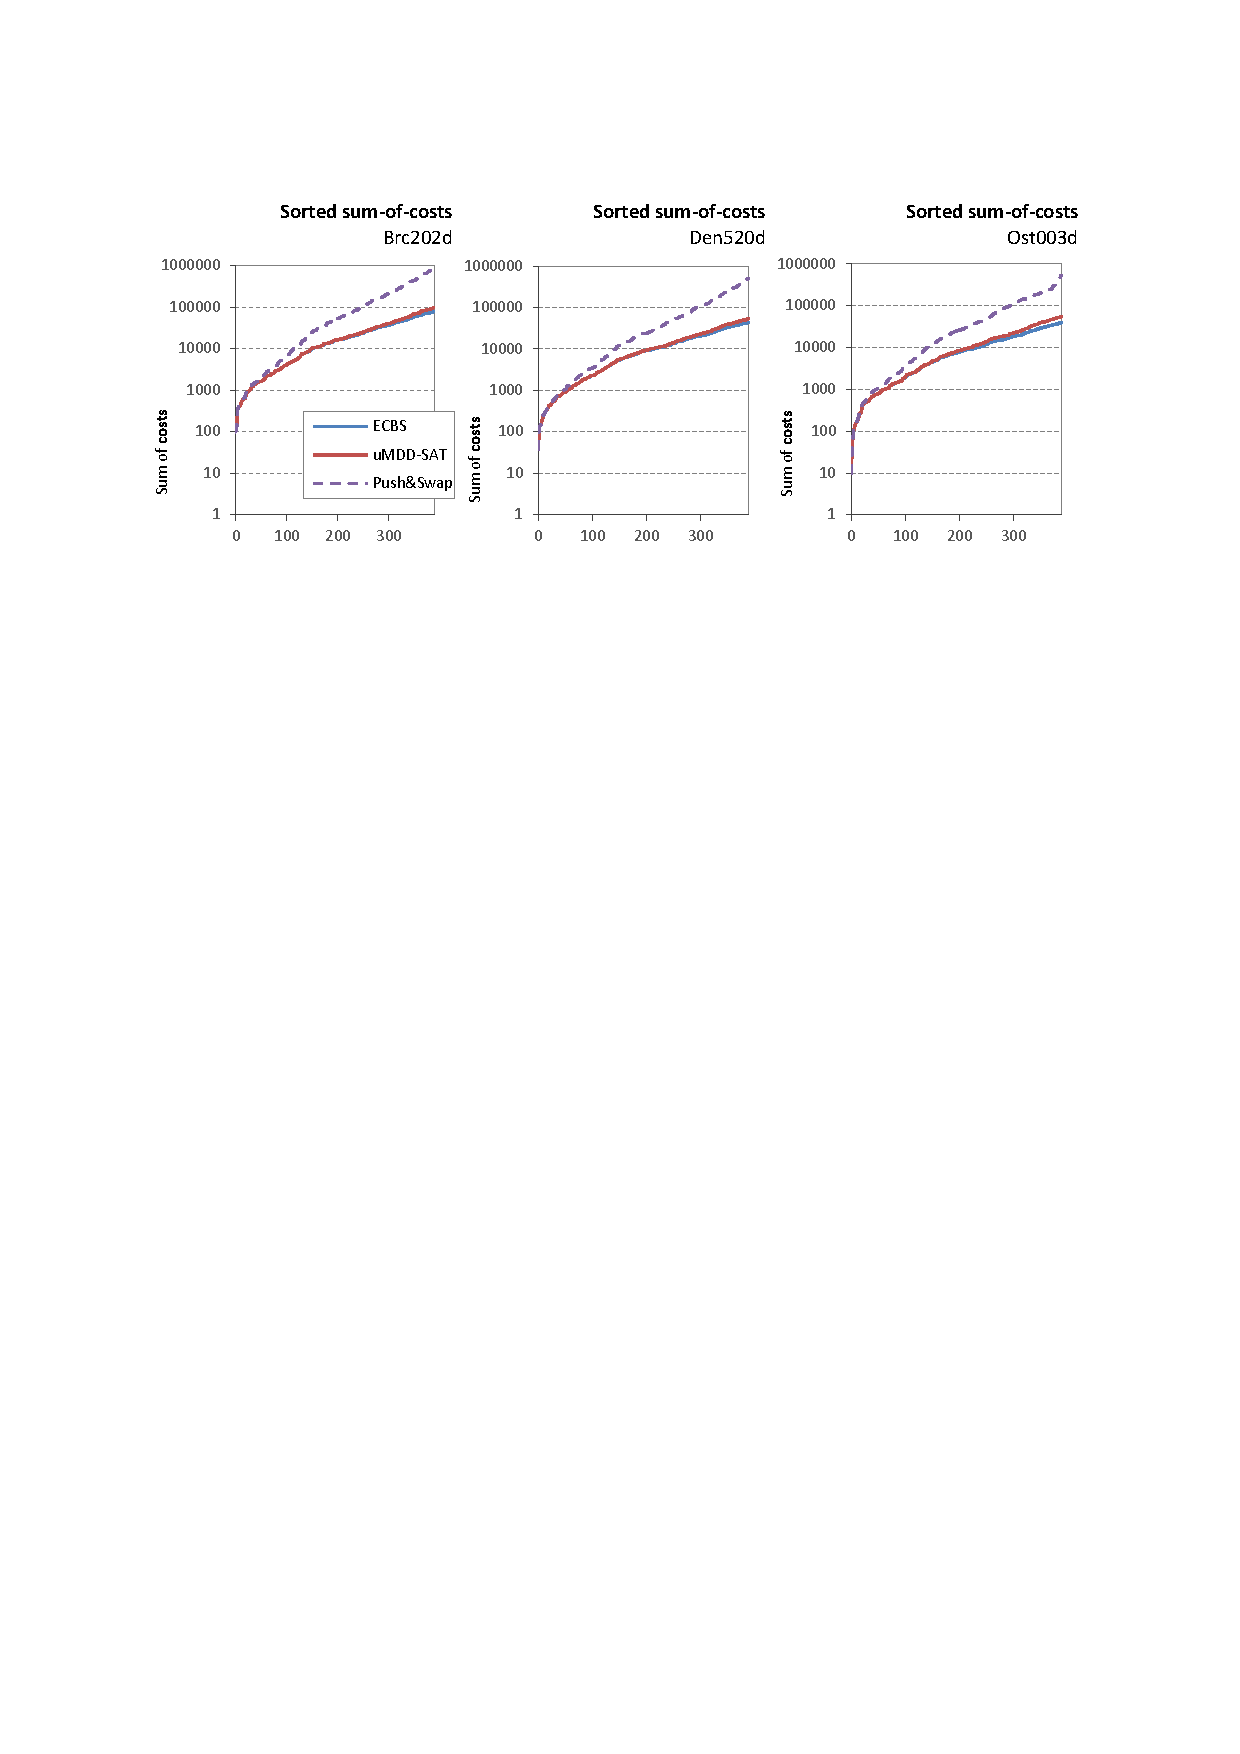
\includegraphics[trim={2.5cm 20.0cm 2.5cm 2.5cm},clip,width=\textwidth]{expr-sub_maps-U-soc-sorted.pdf}
\vspace{-0.8cm}
\caption{Comparison of unbounded suboptimal solvers on DAO maps - sorted sum-of-costs for uMDD-SAT, \textsc{eCbs}, and \textsc{Push-and-Swap}.}
\label{expr-sub_maps-U-soc-sorted}
\end{figure}

\subsubsection{The Bounded Variant: eMDD-SAT}

In test of the bounded variants we used $\epsilon = 0.01$ and tested algorithms eMDD-SAT(1.01) and \textsc{eCbs}(1.01). Both algorithms were tested on small grids with obstacles and large DAO maps. Results are presented in Figures \ref{expr-sub_grids-E-sorted} and \ref{expr-sub_maps-E-sorted} showing sorted runtimes on small grids and large DAO maps respectively.

It can be observed that in small grids eMDD-SAT(1.01) provides better performance than \textsc{eCbs}(1.01). However as the environment gets larger the performance gap between the two algorithms narrows especially in easier instances. The continuation of this trend can be seen in results for DAO maps where \textsc{eCbs}(1.01) dominates except hard instances with many agents.

%\begin{figure}[h]
%\centering
%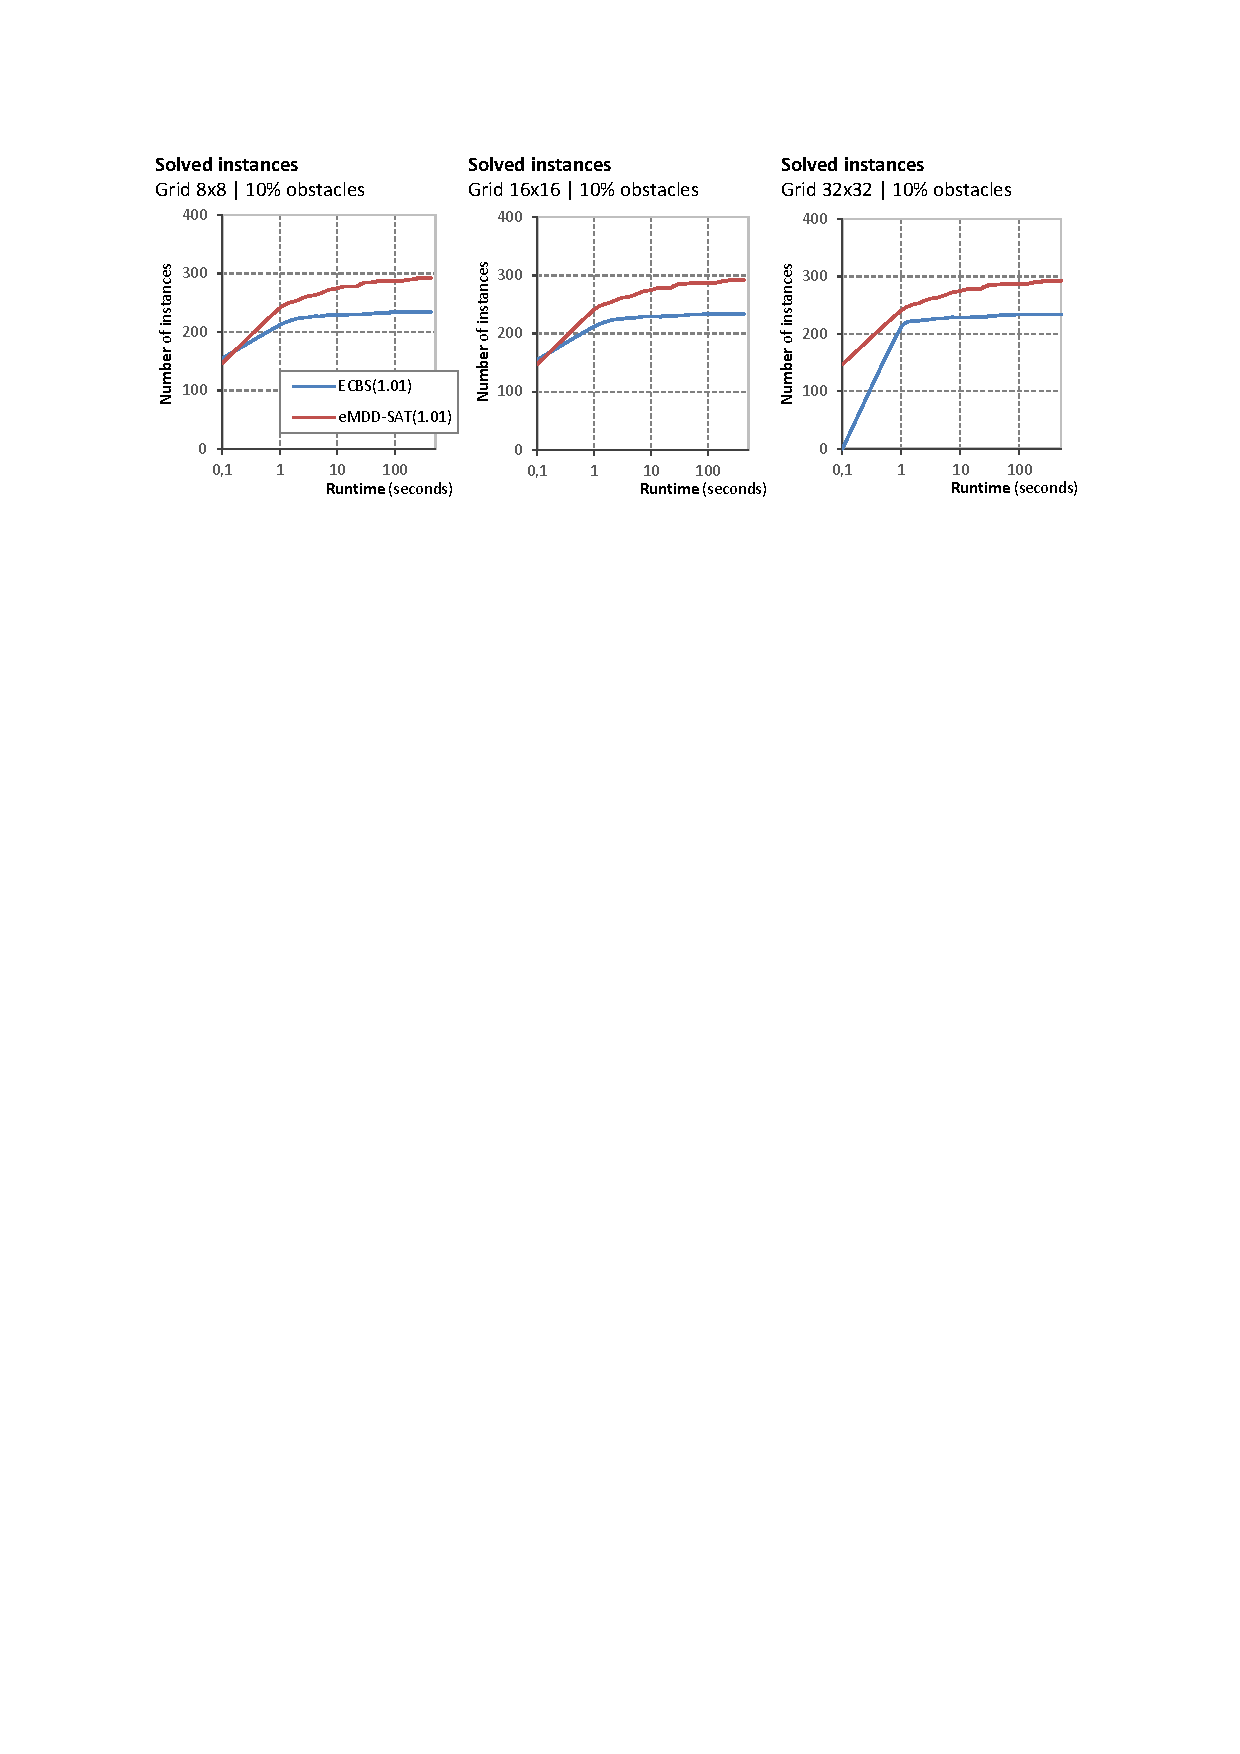
\includegraphics[trim={2.5cm 21.0cm 2.5cm 2.5cm},clip,width=\textwidth]{expr-sub_grids-E-num-solved.pdf}
%\vspace{-0.8cm}
%\caption{Comparison of bounded suboptimal solvers  - number of solvable instances for eMDD-SAT(1.01) and \textsc{eCbs}(1.01) as a function of runtime in $8{}\times{}8$, $16{}\times{}16$, and $32{}\times{}32$ grids (the horizontal runtime axis uses logarithmic scale).}
%\label{expr-sub_grids-E-num-solved}
%\end{figure}

\begin{figure}[h]
\centering
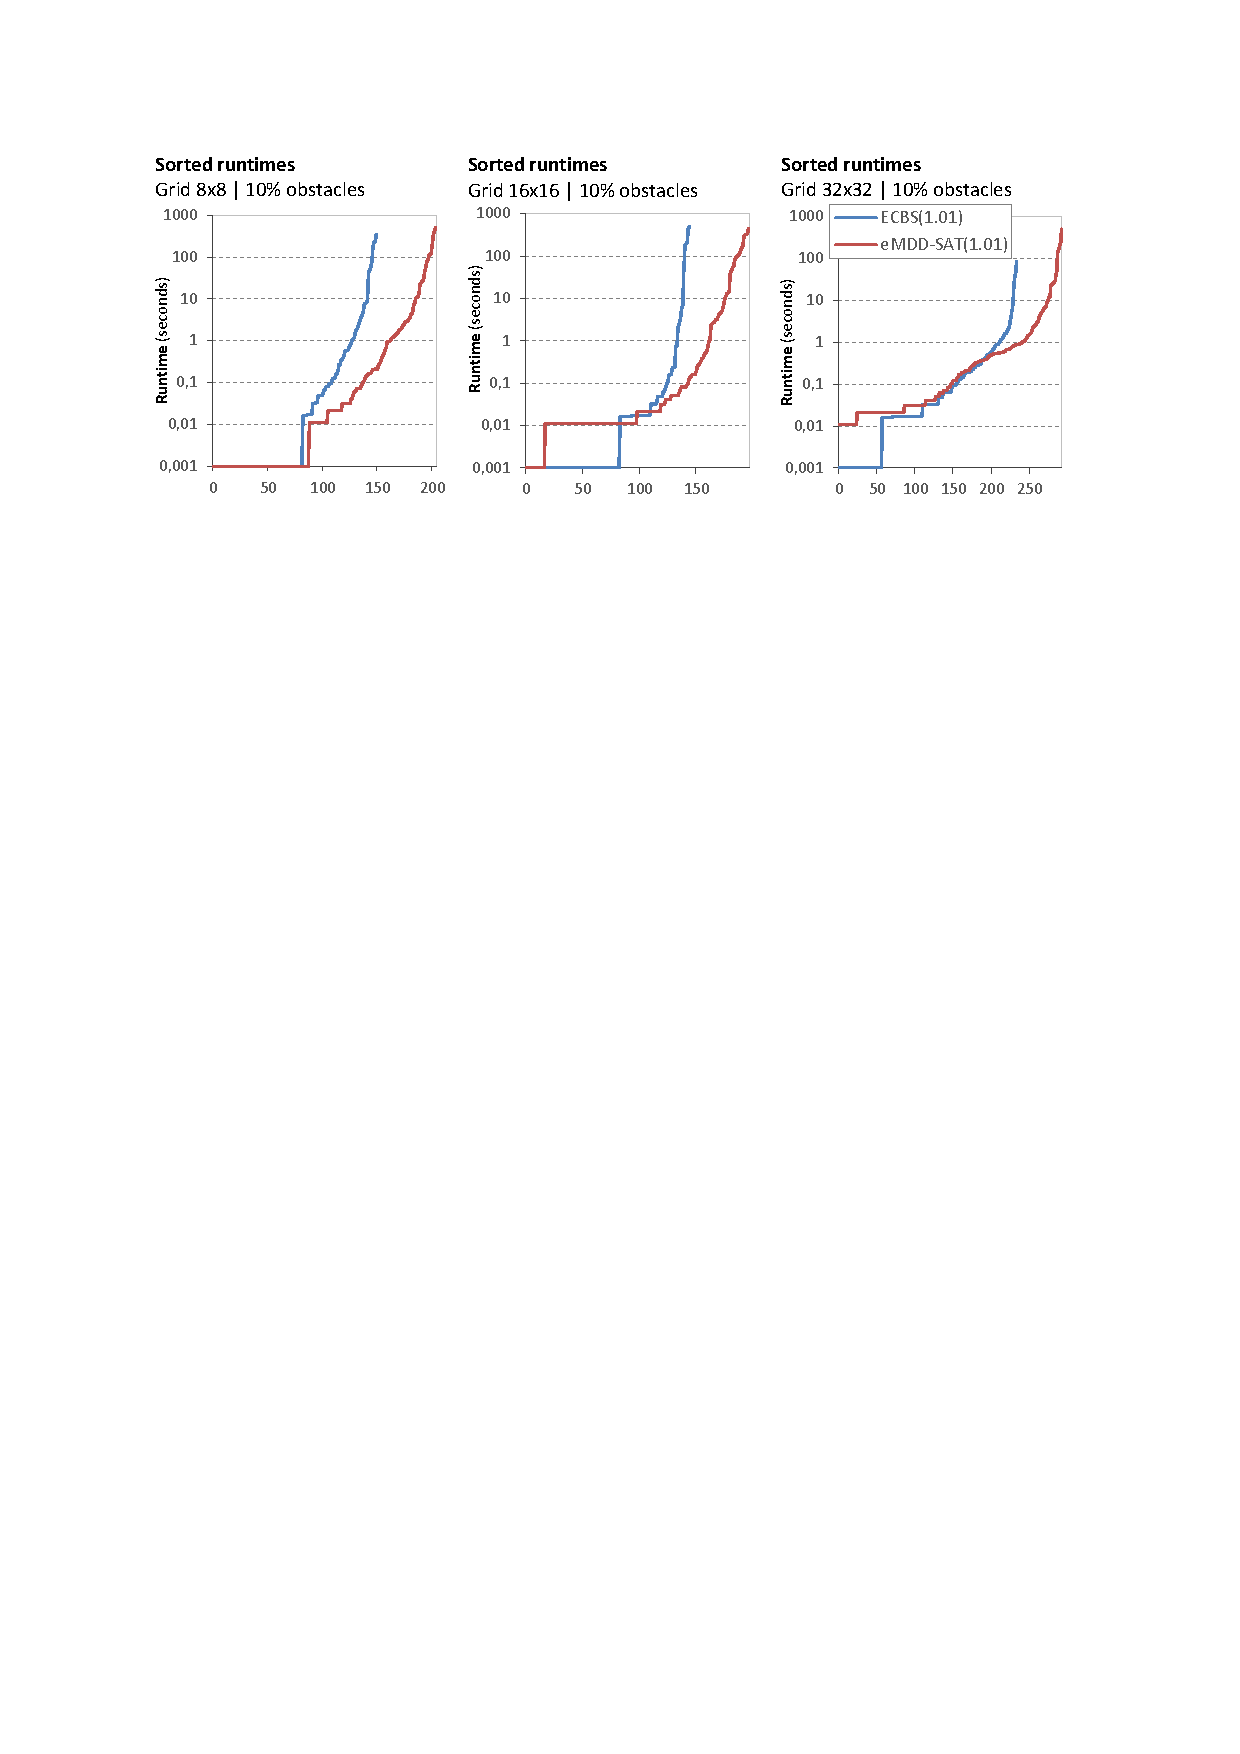
\includegraphics[trim={2.5cm 21.0cm 2.5cm 2.6cm},clip,width=\textwidth]{expr-sub_grids-E-sorted.pdf}
\vspace{-0.8cm}
\caption{Comparison of bounded suboptimal solvers  - sorted runtimes for eMDD-SAT(1.01) and \textsc{eCbs}(1.01)  in $8{}\times{}8$, $16{}\times{}16$, and $32{}\times{}32$ grids.}
\label{expr-sub_grids-E-sorted}
\end{figure}

The explanation for these trends is that once the overhead of constructing MDDs is less significant, eMDD-SAT(1.01) has an advantage over \textsc{eCbs}(1.01). On the other hand if large MDDs are needed to be constructed then eMDD-SAT(1.01) maintains the advantage only for hard cases where \textsc{eCbs}(1.01) cannot find a solution greedily and is forced to perform intensive search while eMDD-SAT(1.01) can use smarter exploration of the search space through learning and Boolean constraint propagation.

%\begin{figure}[h]
%\centering
%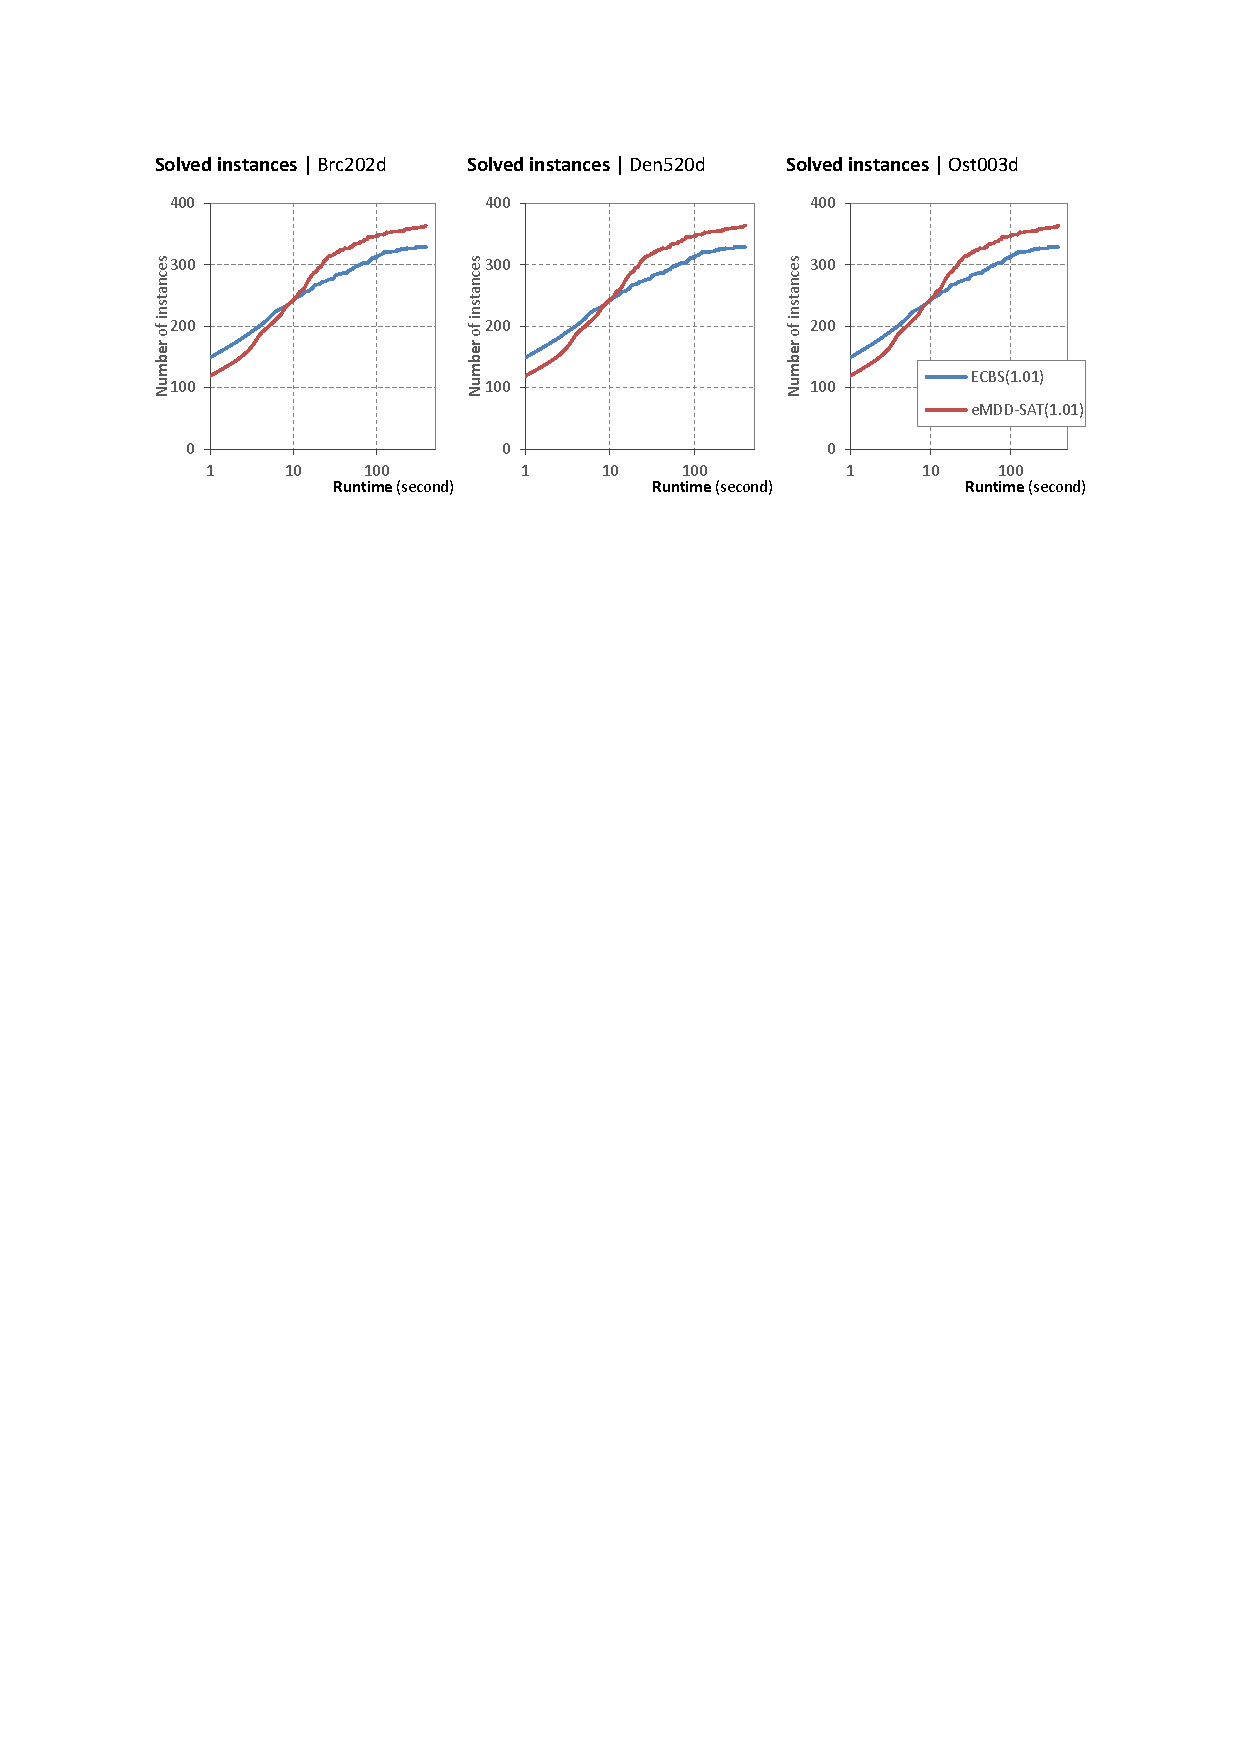
\includegraphics[trim={2.5cm 21.0cm 2.5cm 2.5cm},clip,width=\textwidth]{expr-sub_maps-E-num-solved.pdf}
%\vspace{-0.8cm}
%\caption{Comparison of bounded suboptimal solvers on DAO maps - number of solvable instances for MDD-SAT(1.01) and \textsc{eCbs}(1.01) as a function of runtime (the horizontal runtime axis uses logarithmic scale).}
%\label{expr-sub_maps-U-num-solved}
%\end{figure}

\begin{figure}[h]
\centering
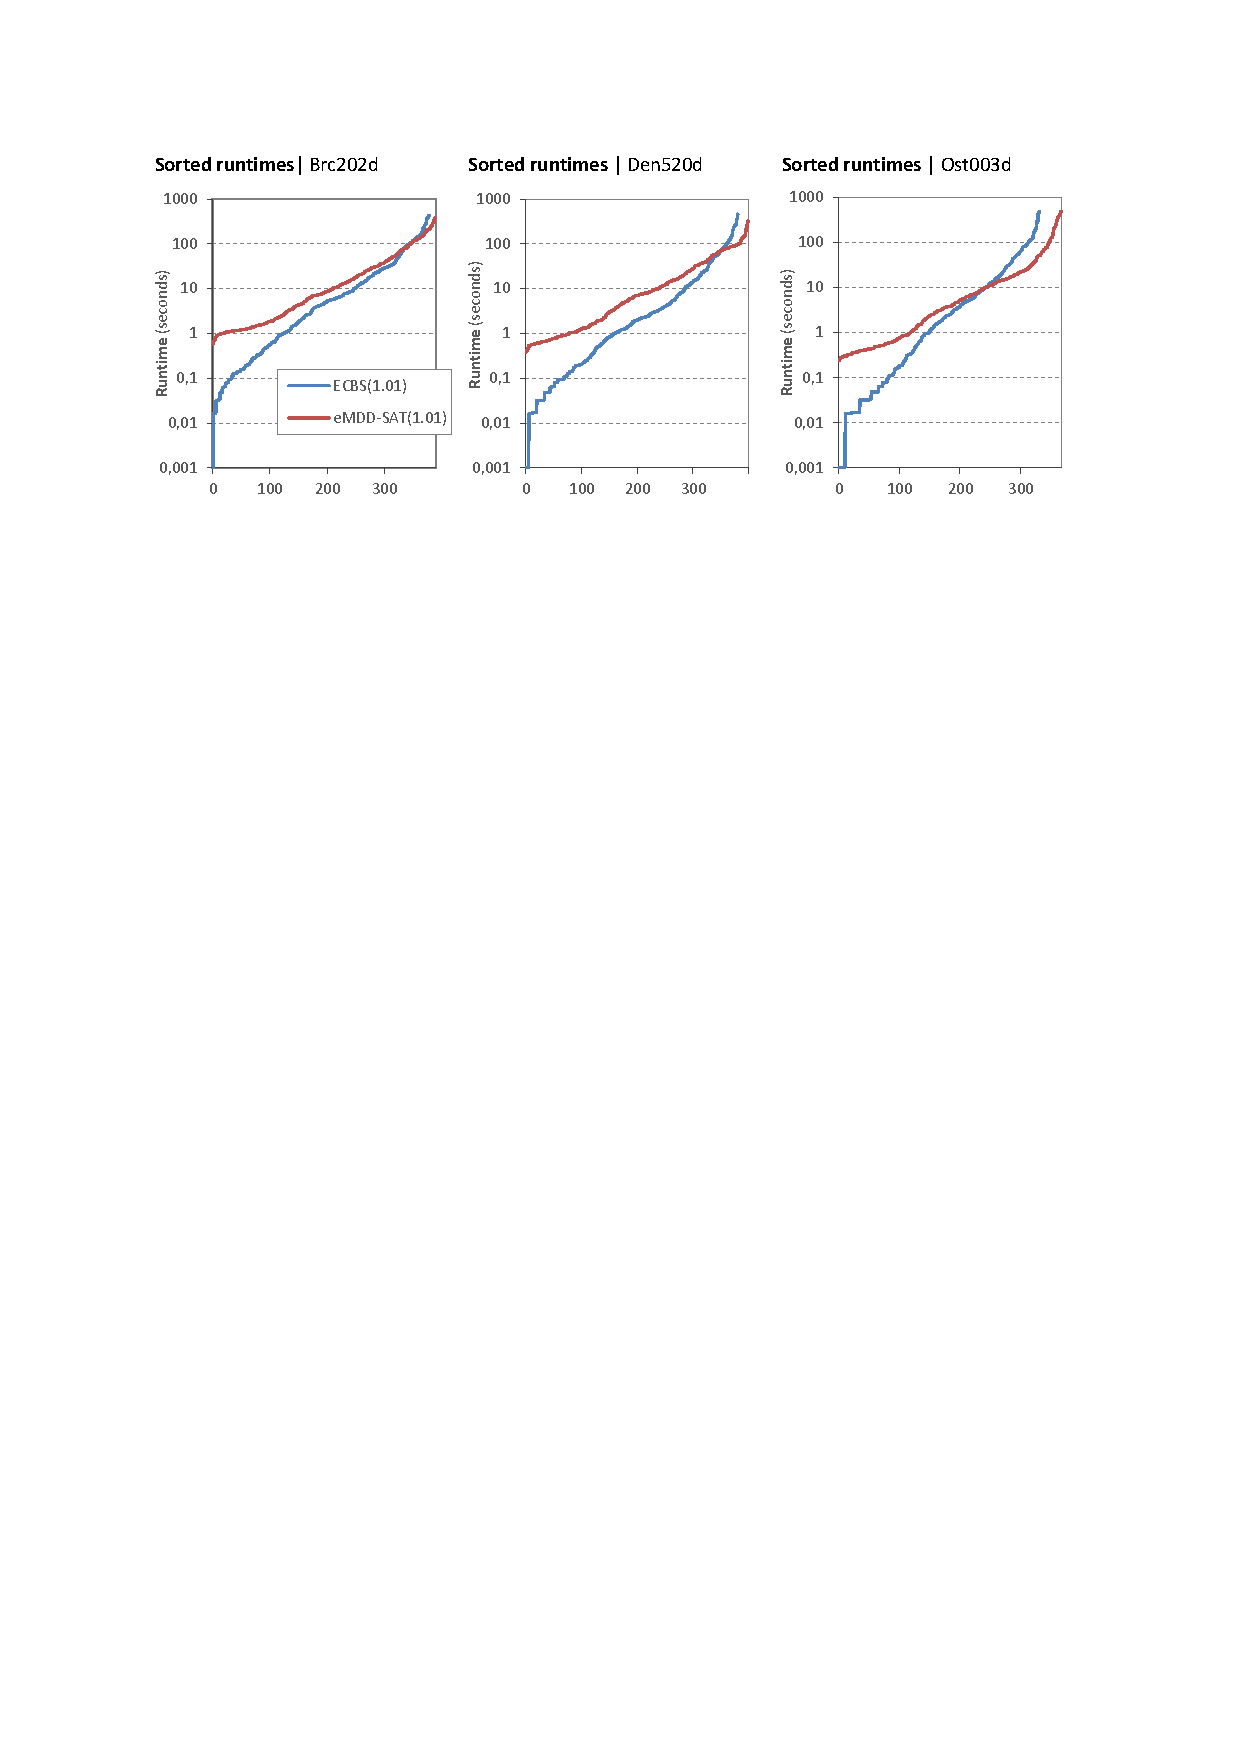
\includegraphics[trim={2.5cm 21.0cm 2.5cm 2.5cm},clip,width=\textwidth]{expr-sub_maps-E-sorted.pdf}
\vspace{-0.8cm}
\caption{Comparison of bounded suboptimal solvers on DAO maps - sorted runtimes for eMDD-SAT(1.01) and \textsc{eCbs}(1.01) are reported.}
\label{expr-sub_maps-E-sorted}
\end{figure}

Additional experiments confirmed that increasing $\epsilon$ generally leads to improving performance of \textsc{eCbs}($1 + \epsilon$) while eMDD-SAT($1 + \epsilon$) relatively looses. Ultimately increasing $\epsilon$ converges to the unbounded case.

\subsubsection{Evaluation of the Number of Time Expansions}
When using the unbounded MAPF solver uMDD-SAT, the actual number of time expansions of MDDs made by the algorithm and the resulting makespan are equal. But as shown in Section \ref{sec:expansions} there is a significant difference between these values when optimal MDD-SAT is used. Hence the natural question is: What is the trend of the difference between the number of MDD expansions and the makespan for bounded suboptimal variants of MDD-SAT depending on error $\epsilon$?

\begin{figure}[h]
\centering
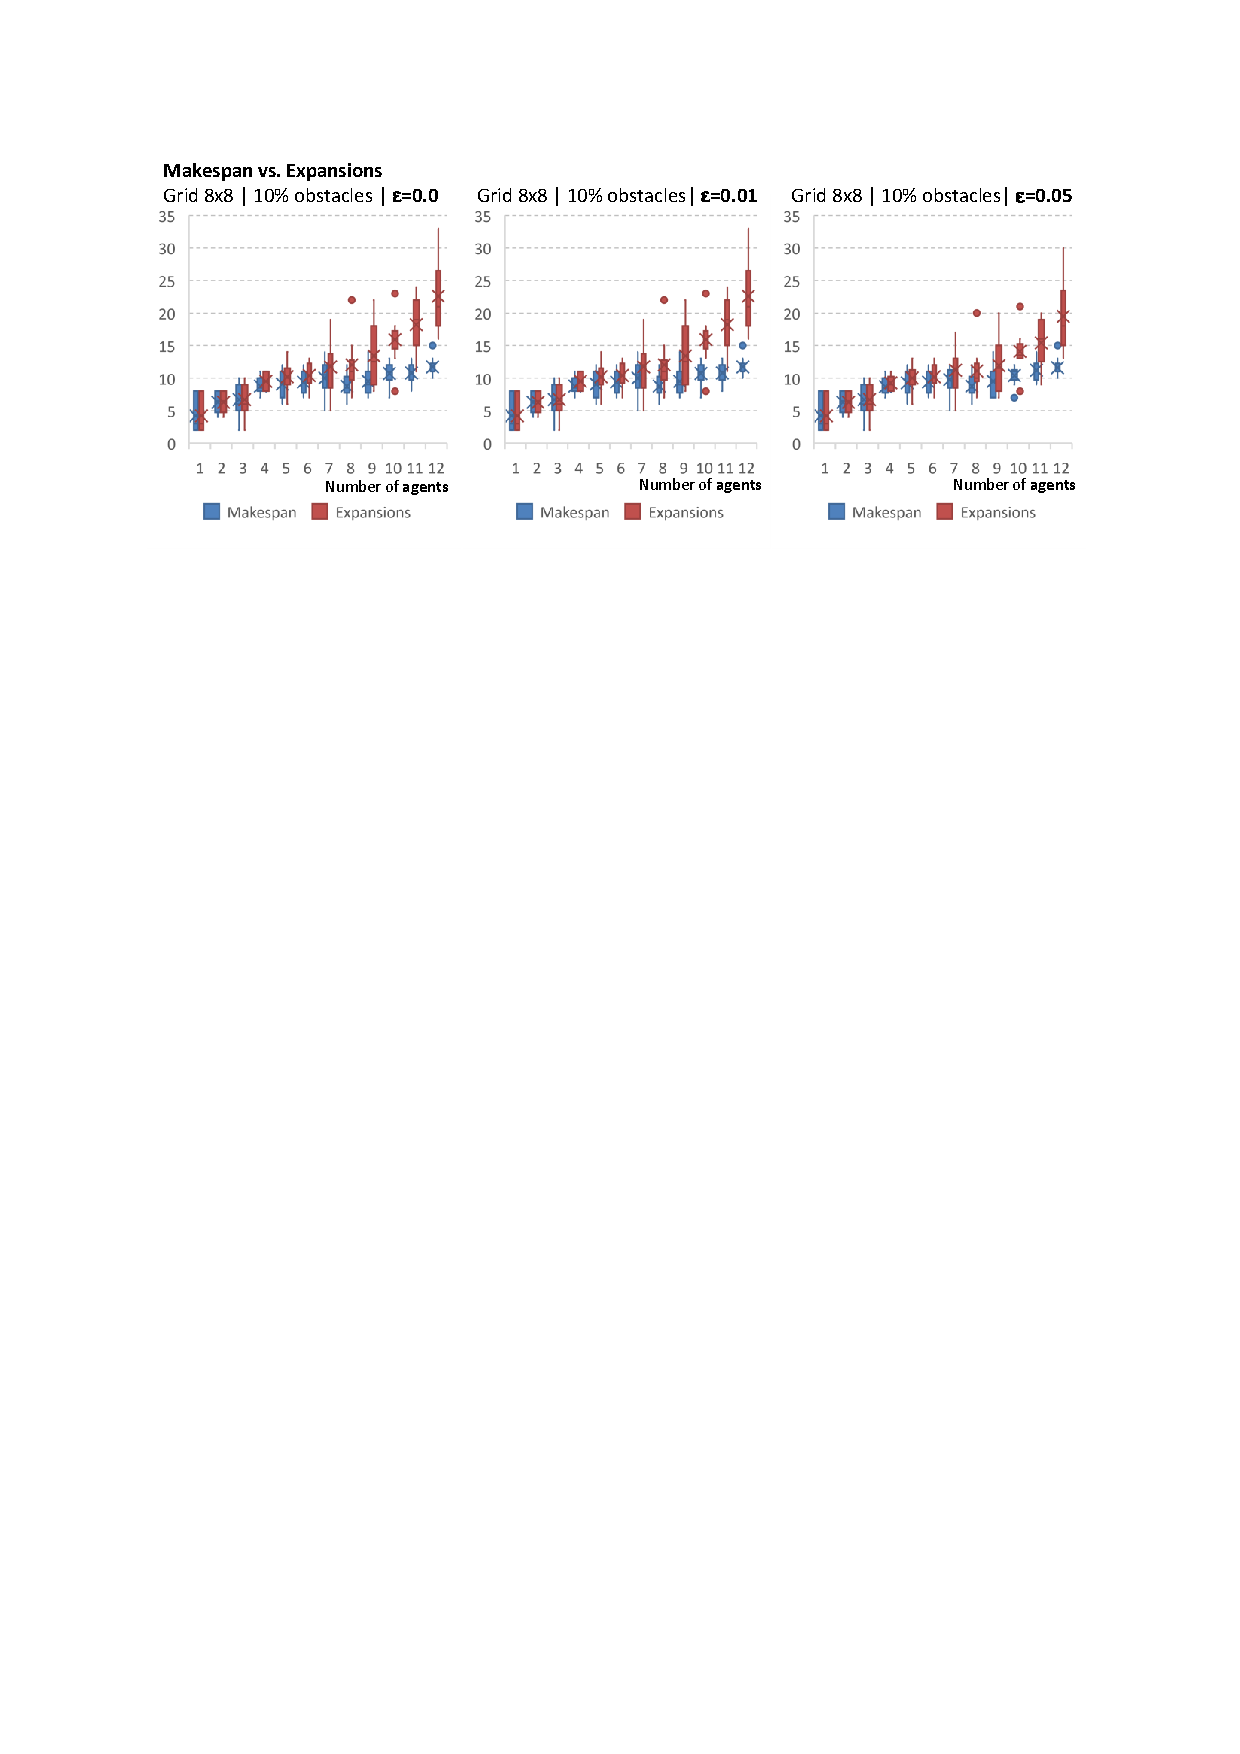
\includegraphics[trim={2.5cm 20.8cm 2.5cm 2.7cm},clip,width=1.0\textwidth]{expr_grids-make-expand_8x8.pdf}
\vspace{-0.6cm}\caption{Comparison of computed makespan and the number of time expansions of MDDs in the $8{}\times{}8$ grid for MDD-SAT, eMDD-SAT(1.01), and eMDD-SAT(1.05).}
\label{figure-make-expand-grids_8x8}
\end{figure}

\begin{figure}[h]
\centering
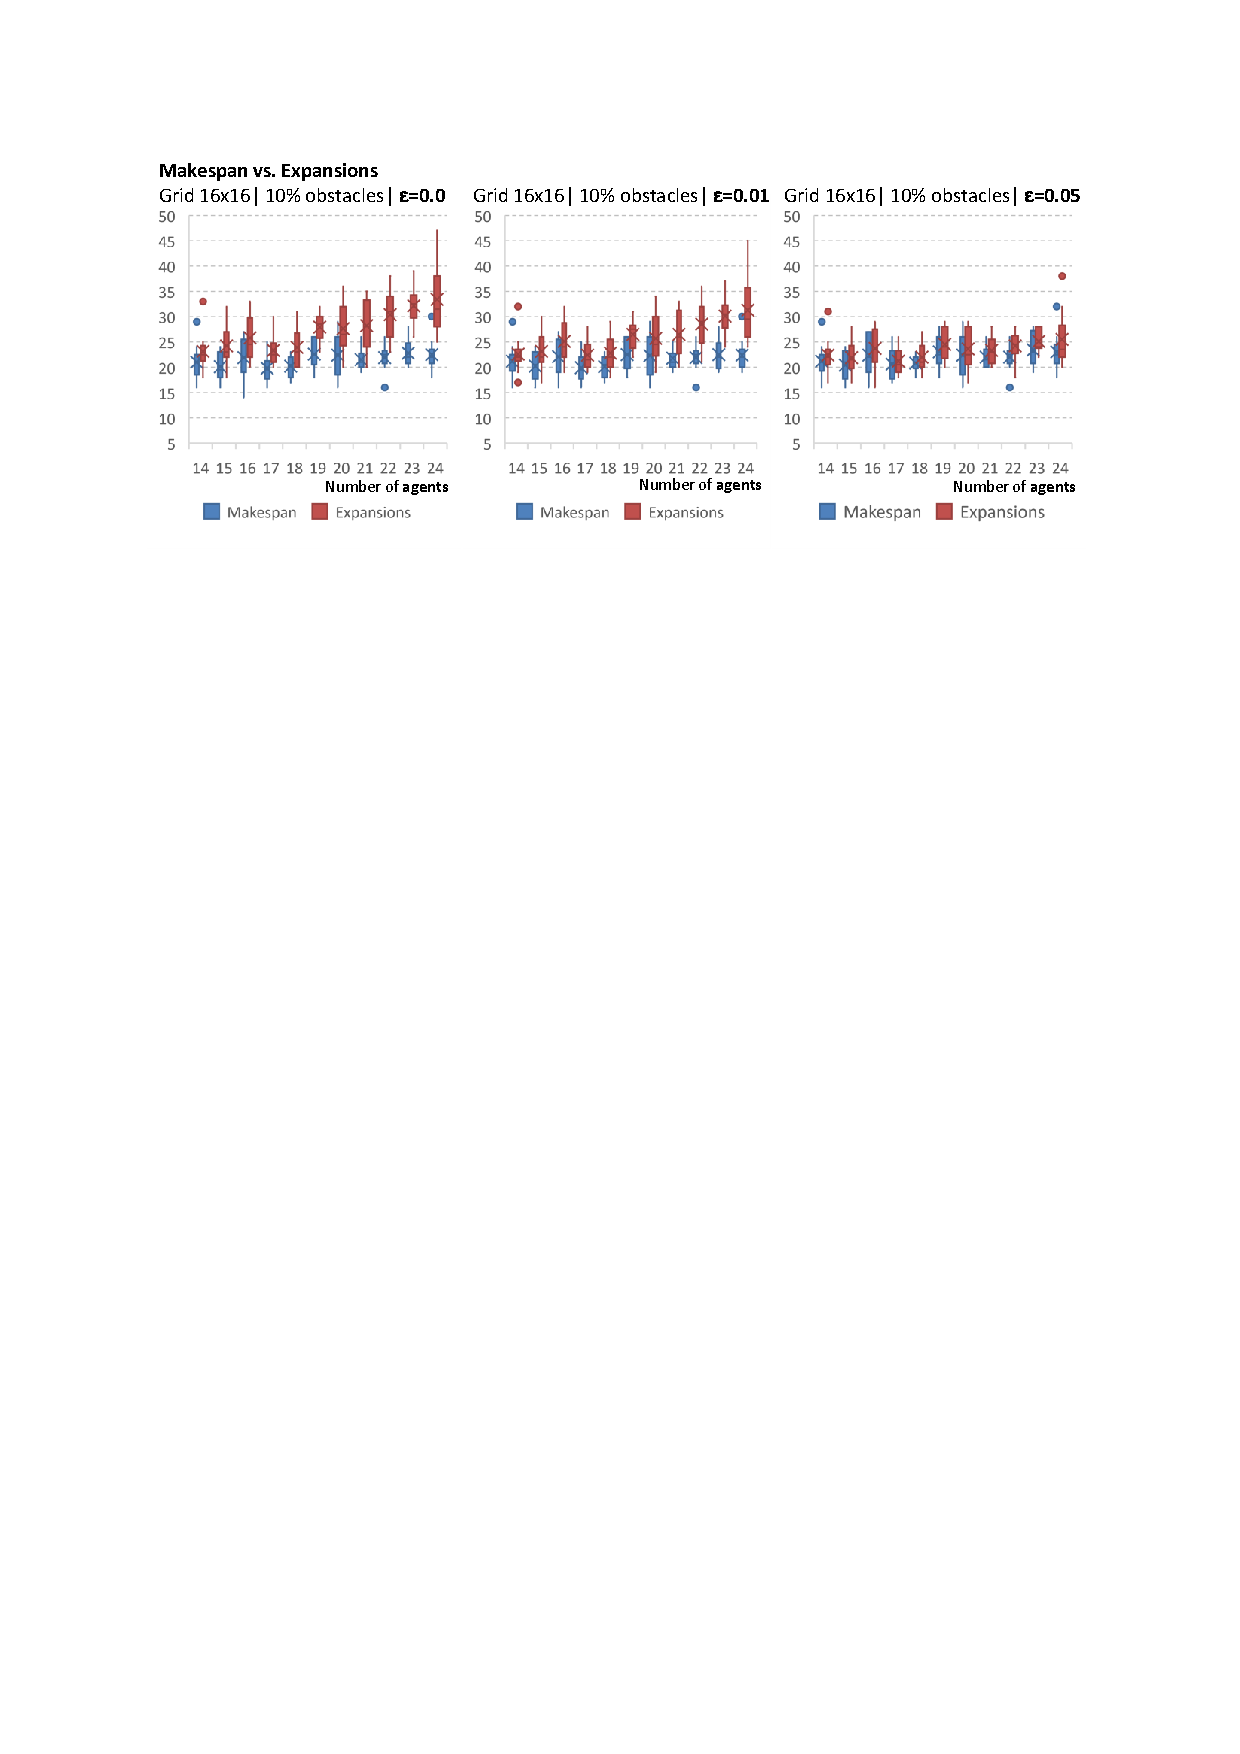
\includegraphics[trim={2.5cm 20.8cm 2.5cm 2.5cm},clip,width=1.0\textwidth]{expr_grids-make-expand_16x16.pdf}
\vspace{-0.6cm}\caption{Comparison of computed makespan and the number of time expansions of MDDs in the $16{}\times{}16$ grid for MDD-SAT, eMDD-SAT(1.01), and eMDD-SAT(1.05).}
\label{figure-make-expand-grids_16x16}
\end{figure}

Results analyzing the difference between the number of expansions and the makespan for grids are shown in Figures \ref{figure-make-expand-grids_8x8}, \ref{figure-make-expand-grids_16x16}, and \ref{figure-make-expand-grids_32x32}. The plots use the same format as in Figures \ref{figure-make-expand-grids_100} and \ref{figure-make-expand-maps_100}, that is a box plot based on 10 random instances per various number of agents is shown. Results for three values of the $\epsilon$ error are shown: $\epsilon=0.0$ (corresponds to optimal MDD-SAT), $\epsilon=0.01$, and $\epsilon=0.05$.

\begin{figure}[h]
\centering
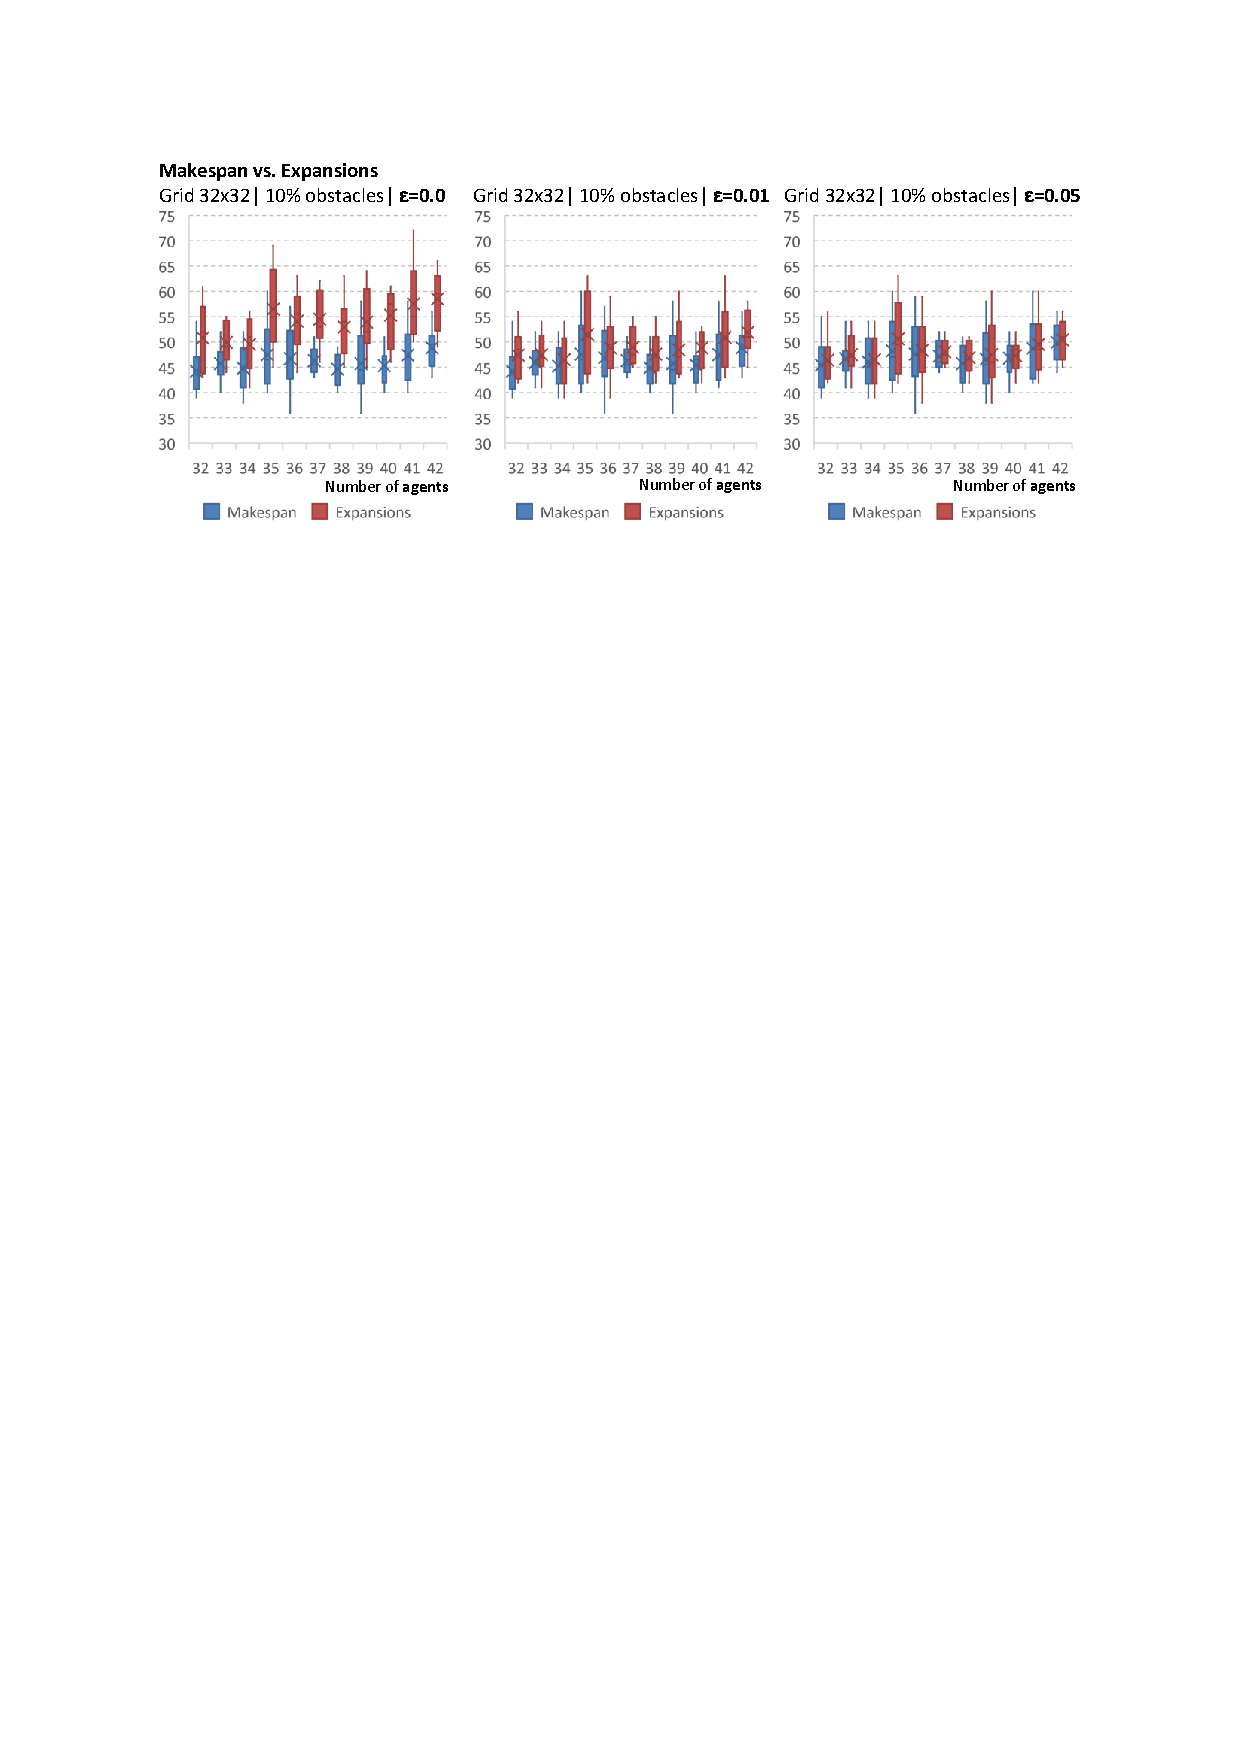
\includegraphics[trim={2.5cm 20.8cm 2.5cm 2.7cm},clip,width=1.0\textwidth]{expr_grids-make-expand_32x32.pdf}
\vspace{-0.6cm}\caption{Comparison of computed makespan and the number of time expansions of MDDs in the $32{}\times{}32$ grid for MDD-SAT, eMDD-SAT(1.01), and eMDD-SAT(1.05).}
\label{figure-make-expand-grids_32x32}
\end{figure}

Results for DAO maps using the same format as results for grids are shown in Figures \ref{figure-make-expand-maps_brc202d}, \ref{figure-make-expand-maps_den520d}, and \ref{figure-make-expand-maps_ost003d}.

A clearly observable trend in the grids is that the difference between the number of expansions and the resulting makespan quickly decreases even for very small increase of $\epsilon$. Moreover, the larger is the grid the convergence of the difference towards zero is faster. The trend is even stronger in DAO maps where the non-zero difference is rare even for the optimal MDD-SAT and quickly diminishes with increased $\epsilon$ in bounded suboptimal eMDD-SAT.

The difference between the number of expansions of MDDs, that equals $\mu_0+\Delta$, and the makespan of computed solution can be regarded through the distribution of extra cost $\Delta$ among agents. When the distribution is unequal, that is, most of the extra cost is consumed by few agents while other agents consume only little in addition to the cost of their shortest paths $\xi_0(a_i)$, then the difference between the number of expansions and the computed makespan is small. On the other hand, when the distribution of the extra cost is distributed equally among the agents, then the difference is large. This is implied by the design of MDD expansion scheme that counts with the worst case when all extra cost is consumed by a single agent.

The factors behind the large difference between the number of expansions and the makespan is first advancing to large extra cost $\Delta$ and second distributing large $\Delta$ equally between the agents so that the distribution is far from the worst case. This situation naturally appears on maps densely occupied by agents (small grids) where agents need to diverge far from their shortest individual paths due to intensive avoidance among each other while it is less common on large DAO maps.

Increasing $\epsilon$ enables the eMDD-SAT algorithm to find a solution with equally distributed extra cost $\Delta$ increased by the $\epsilon$ factor while only making $\mu_0 + \Delta$ expansions which reduces the difference.

\begin{figure}[h]
\centering
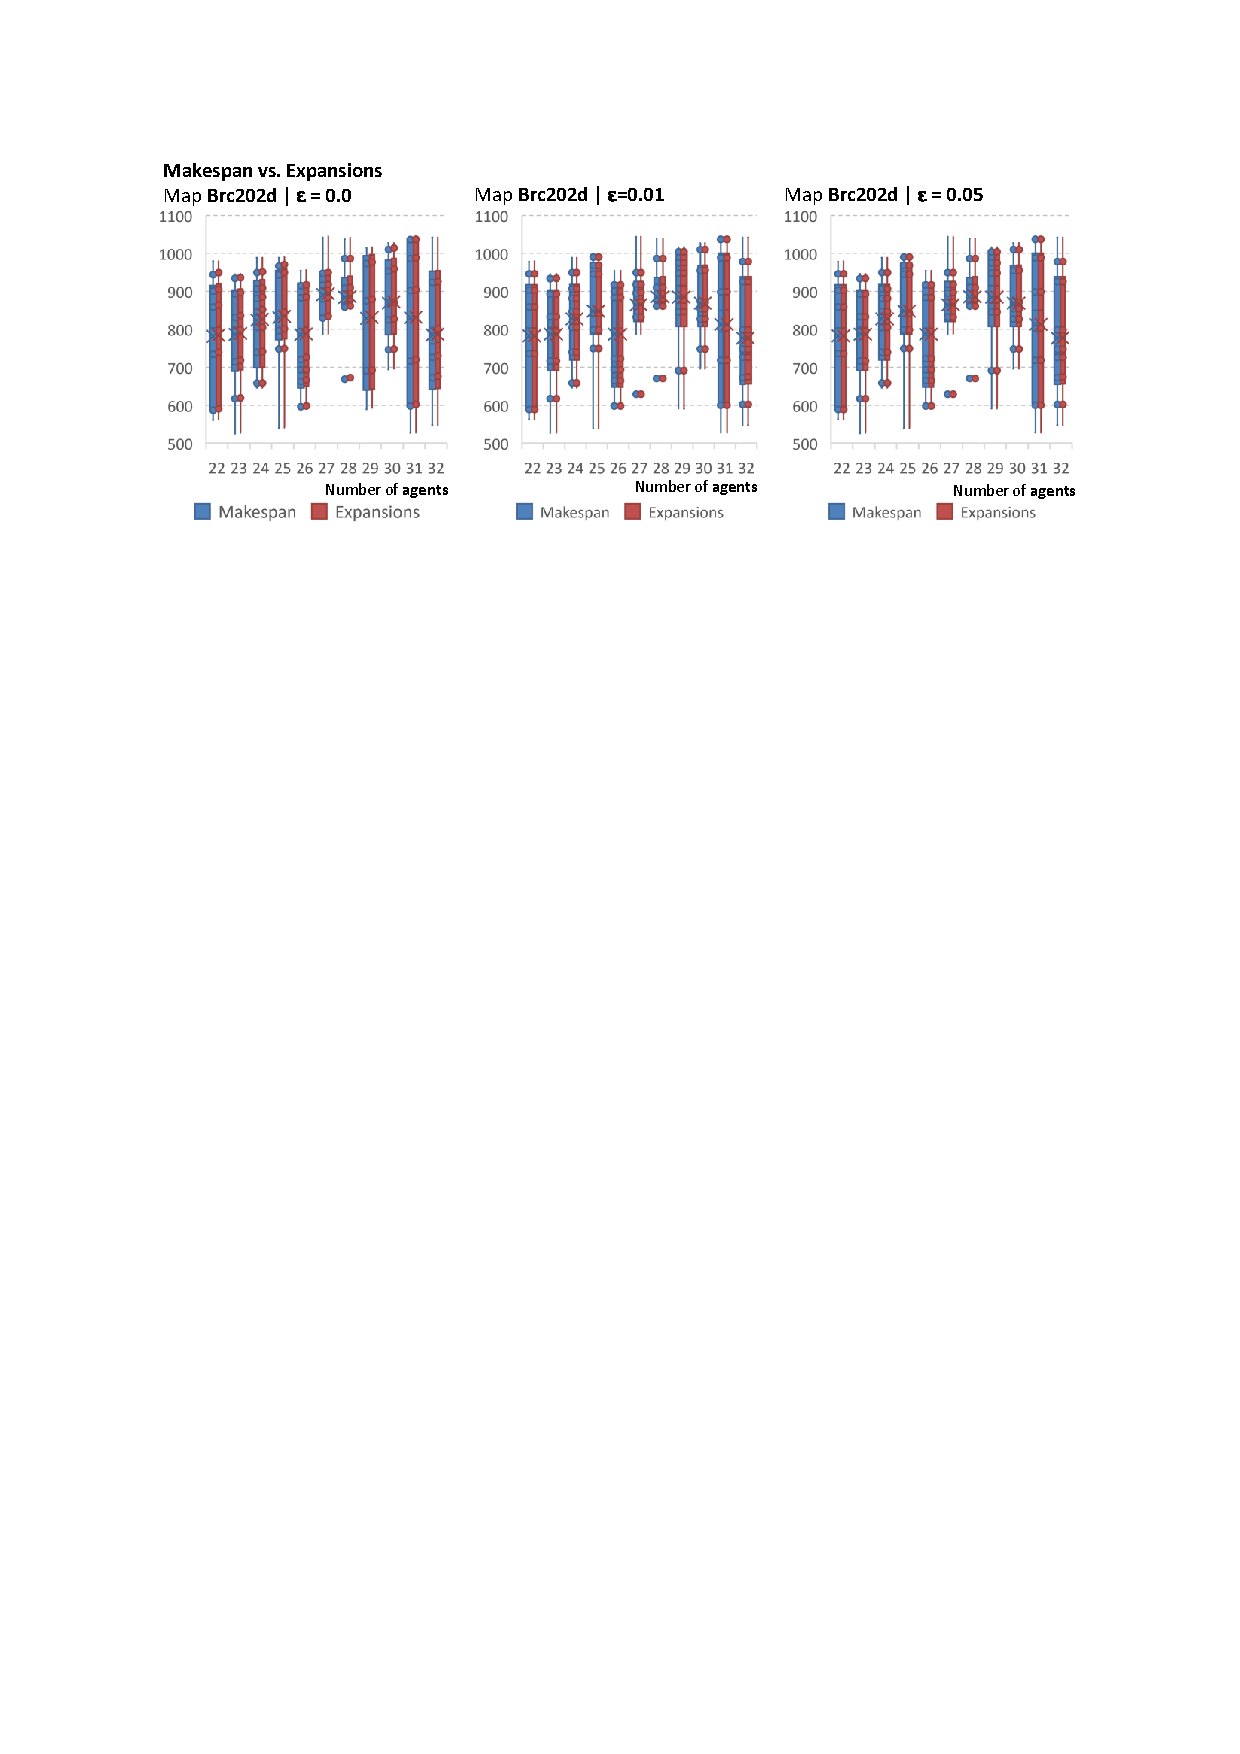
\includegraphics[trim={2.5cm 20.8cm 2.5cm 2.7cm},clip,width=1.0\textwidth]{expr_maps-make-expand_brc202d.pdf}
\vspace{-0.6cm}\caption{Comparison of computed makespan and the number of time expansions of MDDs in DAO map \texttt{brc202d} for MDD-SAT, eMDD-SAT(1.01), and eMDD-SAT(1.05).}
\label{figure-make-expand-maps_brc202d}
\end{figure}

\begin{figure}[h]
\centering
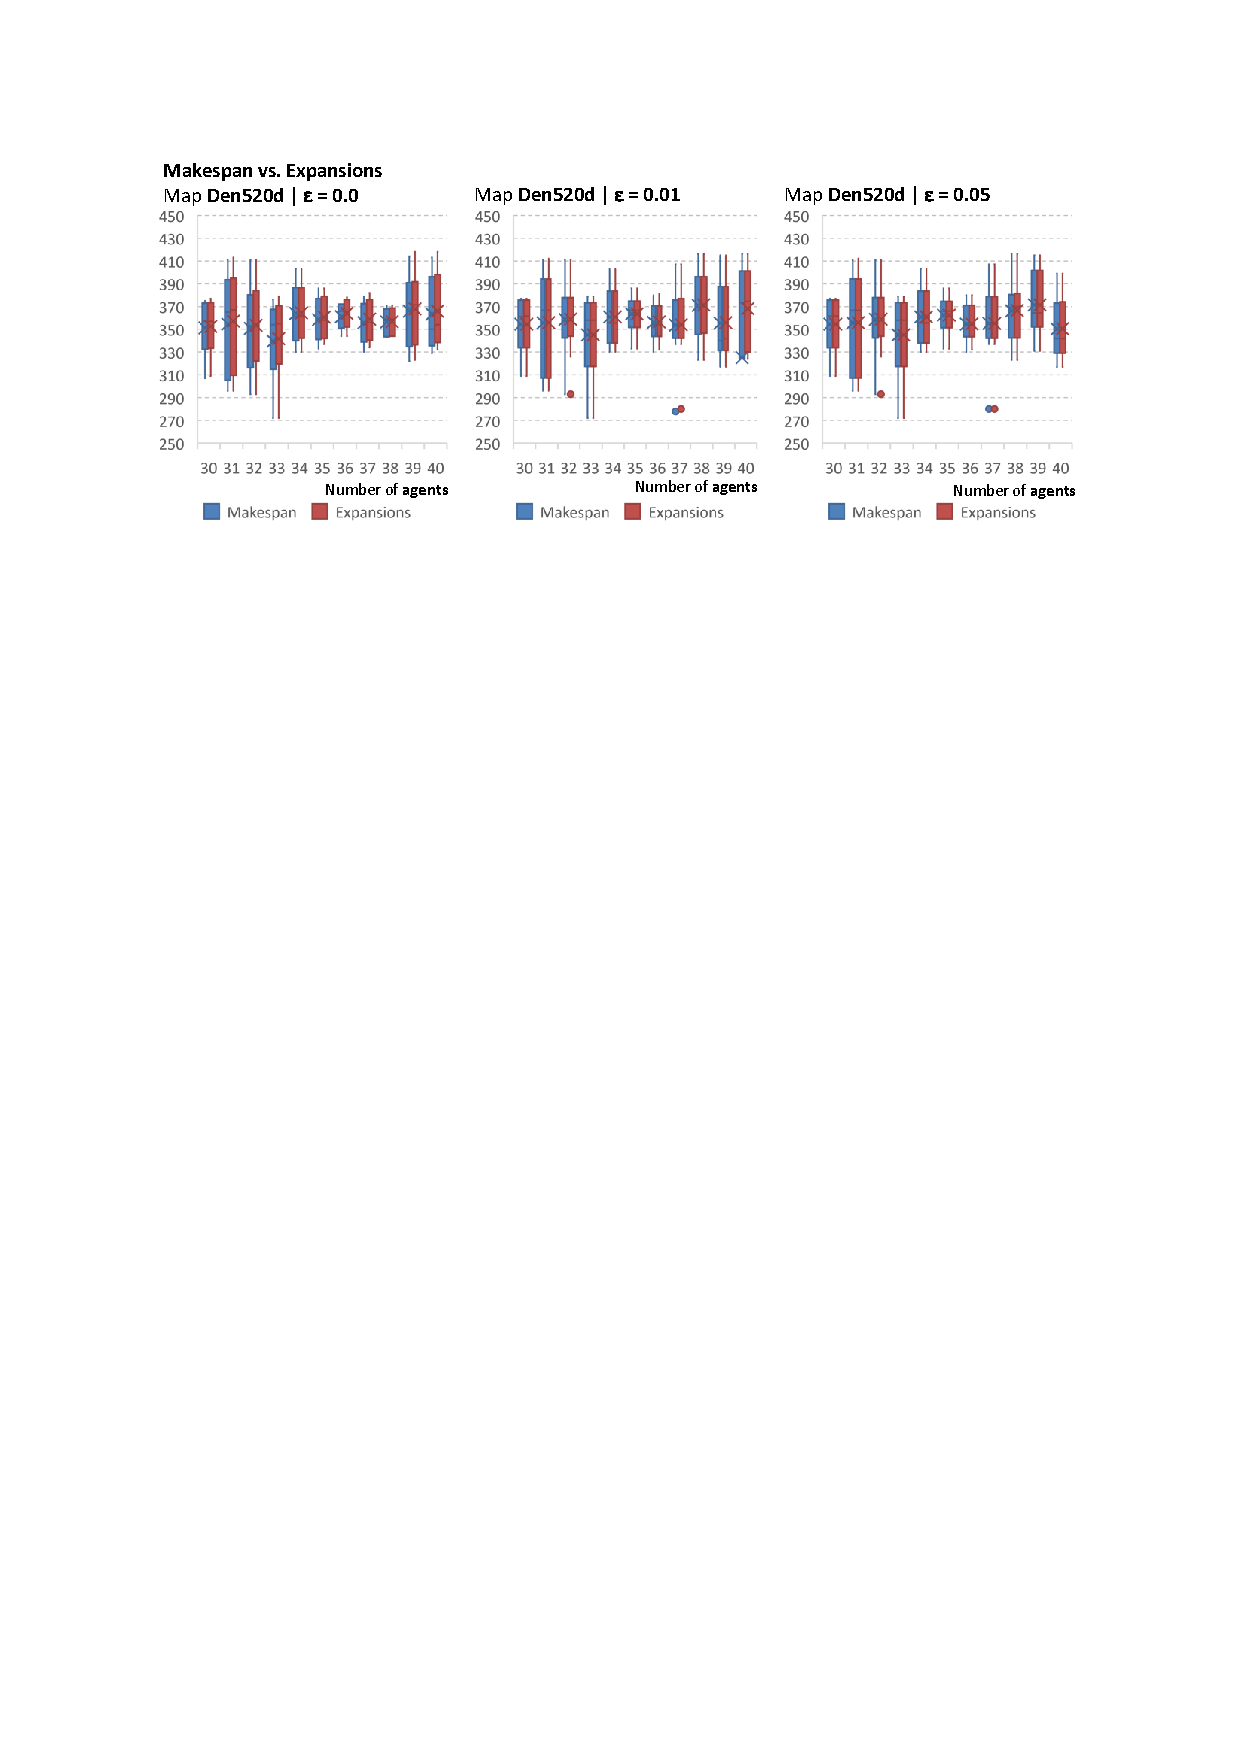
\includegraphics[trim={2.5cm 20.8cm 2.5cm 2.5cm},clip,width=1.0\textwidth]{expr_maps-make-expand_den520d.pdf}
\vspace{-0.6cm}\caption{Comparison of computed makespan and the number of time expansions of MDDs in DAO map \texttt{den520d} for MDD-SAT, eMDD-SAT(1.01), and eMDD-SAT(1.05).}
\label{figure-make-expand-maps_den520d}
\end{figure}

\begin{figure}[h]
\centering
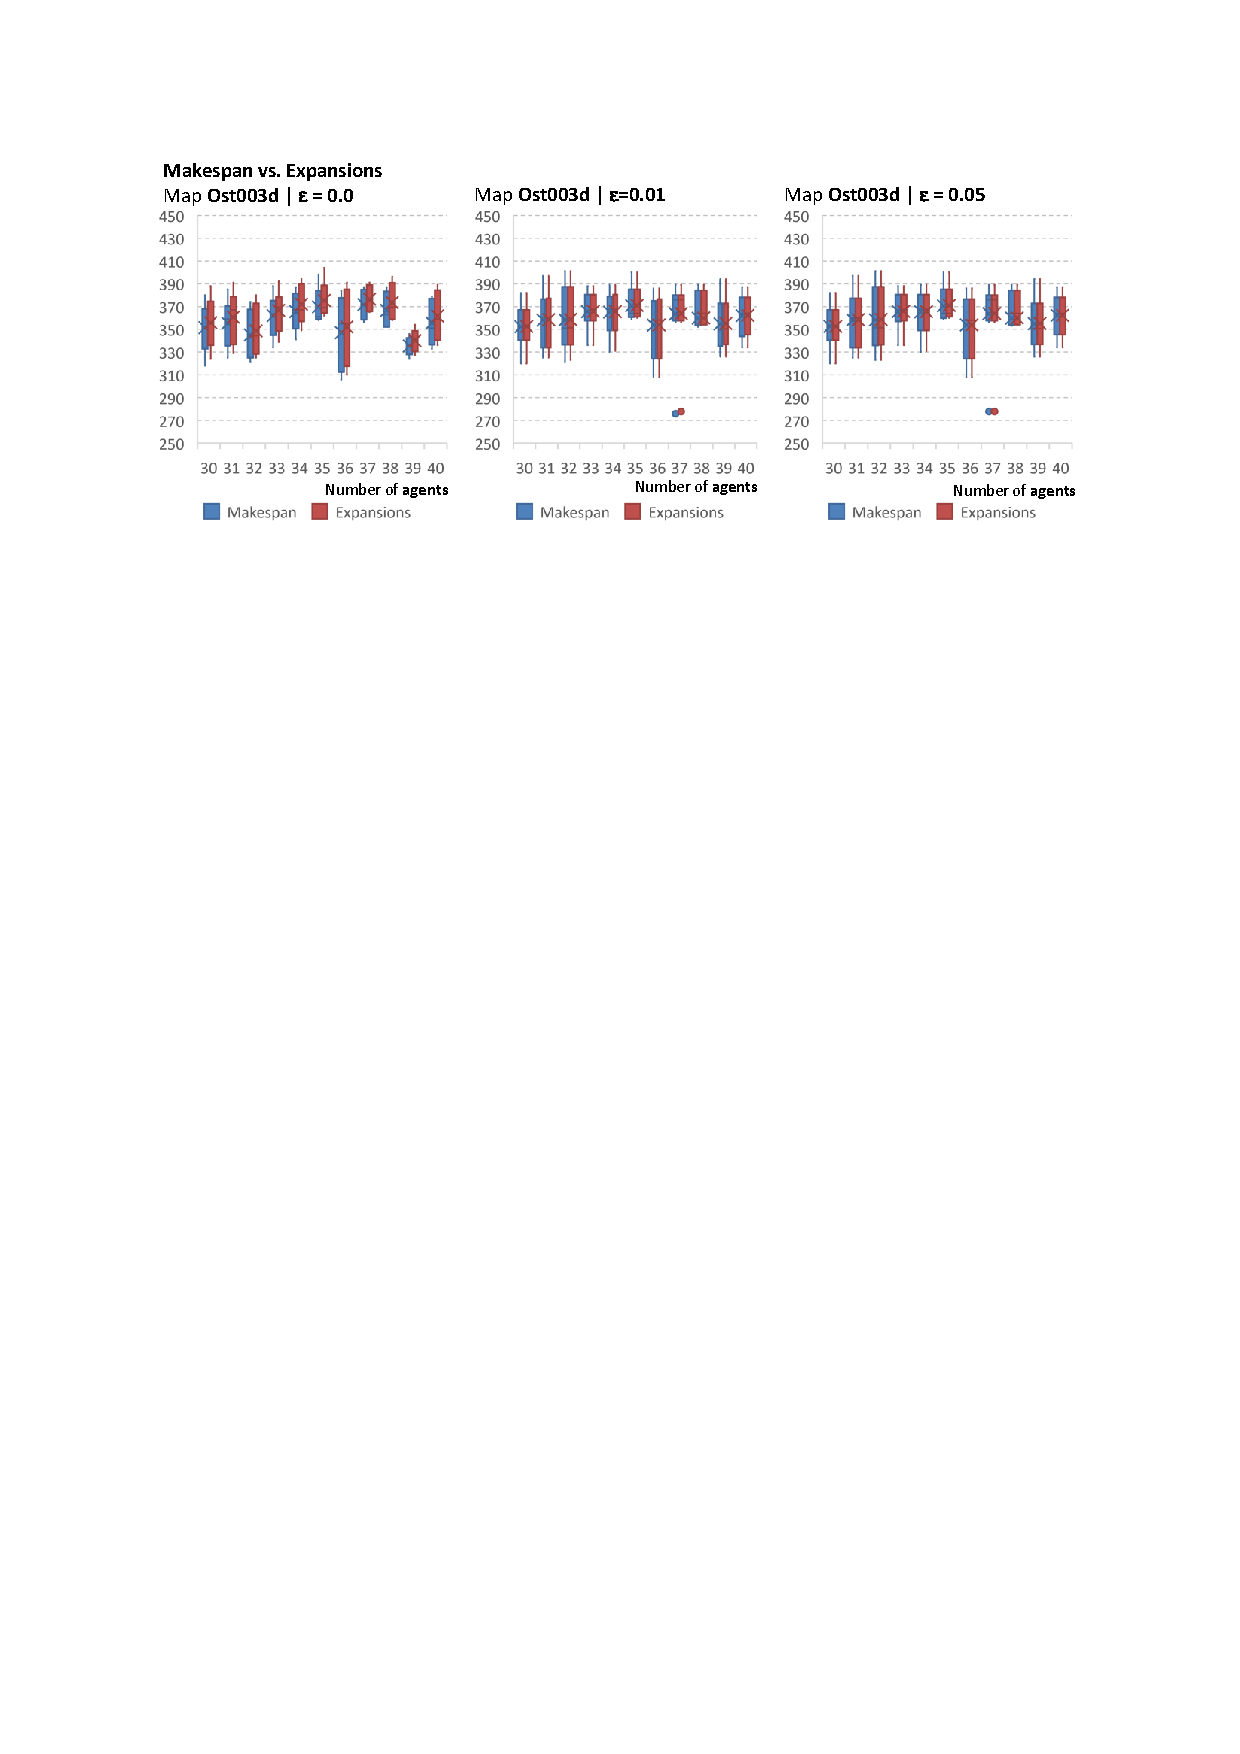
\includegraphics[trim={2.5cm 20.8cm 2.5cm 2.7cm},clip,width=1.0\textwidth]{expr_maps-make-expand_ost003d.pdf}
\vspace{-0.6cm}\caption{Comparison of computed makespan and the number of time expansions of MDDs in DAO map \texttt{ost003d} for MDD-SAT, eMDD-SAT(1.01), and eMDD-SAT(1.05).}
\label{figure-make-expand-maps_ost003d}
\end{figure}

% Tadyma jsem skoncil uz davno

%\section{Discussion}
% Refer variants of MAPF that consider uncertainties, how the SAT-based approach can be transferred for these variants
% Lot of variants and related work have been referred already, it seem to be better to refer no more here



\section{Discussion}

In this paper, we focused on how to migrate techniques from search-based to SAT-based MAPF solvers.
This raises the higher-level question of whether the techniques from MAPF research in general can be migrated to and from other forms of multi-agent planning. 
For example, consider the relation between MAPF and Dec-POMDP~\cite{DBLP:journals/mor/BernsteinGIZ02,DBLP:conf/aaai/OliehoekWK12,Witwicki2011,DBLP:conf/aips/WitwickiD10,DBLP:conf/aips/VarakanthamKTMST09,DBLP:journals/jair/BeckerZLG04}. 
Briefly, MAPF can be viewed as a special case of Dec-POMDP where the agents are fully observable, all action outcomes are deterministic, and the actions of each agent is just to move to an adjacent cell. In MAPF, the agents’ goal is to reach their corresponding goal positions, while in Dec-POMDP the goal is to maximize a joint reward function. In MAPF, the only interaction between the agents is negative, i.e., agents cannot help each other to achieve their goals, that is, adding agents can only make the problem solving harder. In contrast, in Dec-POMDP agents may assist each other, and having more agent may yield higher reward. In both cases, however, a major speedup can be obtained by decoupling the planning process as much as possible. The ID framework is one such example in MAFP, while all the mentioned references are examples of doing this for Dec-POMDP. Technically, in MAPF transitions are not independent, since agents may collide with each other. The reward function for the sum of costs is independent, as it adds one unit cost per movement of each agent. 

% Identifying coordination locals in MAPF is a very interesting topic for future work.
% Pavel: what is "local in MAPF"?
% Future work, non-unit costs and their processing via cardinality constraits.

In particular, the technique of independence detection (ID) is not limited to MAPF setting. 
ID in the MAPF setting considers local interactions between agent groups through collisions while collisions can be understood as a form of local interactions that altogether compose a network of interactions. 

More general approaches for dealing with networks of interactions have been developed in multi-agent planning (MAP), especially in MAP under uncertainty addressed via partially observable Markov decision processes (POMDPs) \cite{DBLP:conf/aaai/NairVTY05}. Finding optimal policies in POMDPs is a computationally hard problem in general, hence various techniques that simplify the problem via exploiting the structure of the interaction network have been developed. Specifically local independence such as {\em observation independence} and {\em transition independence} can be used for more efficient policy generation for POMDPs. Important concept for analyzing dependencies among agents is represented by {\em coordination graphs} \cite{DBLP:conf/nips/GuestrinKP01,DBLP:conf/aaai/GuestrinVK02} that can be used to decompose the problem into smaller independent parts for which the policy generation is easier.

The assumption in the MAPF setting is that suitable actions for agents are being determined so that collisions are avoided and agents maximize their objective, that is, they head towards their goal positions. In contrast to this, different MAP approaches do not explicitly assume what are the correct actions leading to achieving the objective but instead agents learn suitable actions via reinforcement learning during the planning process \cite{DBLP:journals/jmlr/KokV06}.

Another important question is how to extend this work in the context of recent research of the interaction of SAT-based and search-based MAPF solvers. Contemporary studies indicate that SAT-based and search-based solvers are complementary in terms of suitability for certain types of MAPF \cite{DBLP:conf/aips/KaduriBS20,kaduri2021experimental}. That is, there exist types of MAPF instances in which the SAT-based approach dominates the search-based one and vice versa. These studies suggest that a more sophisticated portfolio-based solvers for MAPF could be a promising research direction.

\section{Conclusion}

The paper summarizes MDD-SAT, the first state-of-the-art SAT-based solver for the sum-of-costs variant of MAPF.  We explain in details ideas necessary to reach the resulting enhanced propositional encoding that migrates the ideas from the search-based methods for the use by SAT solvers. MDD-SAT was experimentally compared to state-of-the-art search-based solvers over a variety of domains such as 4-connected grids with random obstacles and large maps from computer games. Our results show that MDD-SAT is often the better option in hard scenarios, while the search-based solvers may perform better in easier cases.

Nevertheless, there is no universal winner and each of the approaches has pros and cons and thus might work best in different circumstances. This calls for a deeper study of various classes of MAPF instances and their characteristics, and how the different algorithms behave across them. Although early studies were made, not too much is known at present to the MAPF community about these aspects.

% \cite{DBLP:conf/aips/KaduriBS20,kaduri2021experimental} moved to the last paragraph in the discussion

There are several factors behind the performance of the SAT-based approach: clause learning, constraint propagation, and an efficient implementation of the SAT solver. On the other hand, the SAT solver does not understand the structure of the encoded problem which may downgrade the performance. Hence, we consider that implementing techniques such as learning directly into the dedicated MAPF solver may be a future direction.

% as previous authors mentioned~\cite{CBSJUR,DBLP:conf/ijcai/BoyarskiFSSTBS15}

%Although early studies were made \cite{DBLP:conf/aips/KaduriBS20,kaduri2021experimental} not too much is known at present to the MAPF community about these aspects. 

% We could cite my recent papers on algo. selection for this
% Pavel: please check if the citation is correct, feel free to reformulate

Versatility of SAT-based approach is further demonstrated through integrating the independence detection technique into the MDD-SAT solver and by introducing the unbounded suboptimal and the bounded suboptimal variants of the solver. In both modifications of the basic solver, we obtained analogous results as in the case when these modifications were carried out for search-based solvers. Independence detection in MDD-SAT helps significantly when there is little interaction between agents. Suboptimal variants of MDD-SAT enables trading the solution quality for the runtime.

For our future work we plan to use the SAT solver more actively during the construction of propositional encoding. Mechanisms that build the encoding and simultaneously check its satisfiability seem to be of great potential. Another direction for future work is to develop efficient encodings for MAPF problems beyond classical MAPF, e.g., where edges have non-uniform costs. 

% \cite{DBLP:conf/ijcai/Surynek19}

\section*{Acknowledgments}

This research was supported by the Czech Science Foundation (GA\v{C}R), the grant registration number 19-17966S.

\begin{small}
\end{small}

\bibliography{JOURNALmapf}
\bibliographystyle{theapa}

\end{document}
\endinput

